\documentclass{memoir}
\usepackage[utf8x]{inputenc}
\usepackage{ucs}
\usepackage[spanish,es-tabla]{babel}
\usepackage{mathpazo}
\usepackage{courier}
\usepackage{textcomp}
\usepackage{amsmath}
\usepackage{amssymb}
\usepackage{xcolor}
\usepackage{listingsutf8}
\usepackage{parskip}
\usepackage{array}
\usepackage{booktabs}
\usepackage{ctable}
\usepackage{enumitem}
\usepackage{hyperref}
\usepackage{microtype}

\usepackage{tikz}
\usetikzlibrary{calc,shapes,arrows}
\tikzstyle{decision} = [
  diamond,
  very thick,
  draw=red!50!black!50,
  %fill=red!20, 
  aspect=2,
  %text badly centered,
  top color=white,
  bottom color=red!50!black!20,
]
\tikzstyle{stmt} = [
  rectangle,
  very thick,
  draw=blue!50!black!50,
  %fill=blue!20, 
  text centered,
  minimum height=5ex,
  minimum width=5em,
  top color=white,
  bottom color=blue!50!black!20,
]
\tikzstyle{node} = [
  circle,
  very thick,
  draw=orange!50!black!50,
  fill=orange!20,
  minimum size=6ex,
]
\tikzstyle{io} = [
  very thick,
  draw=green!50!black!50,
  trapezium,
  trapezium left angle=80,
  trapezium right angle=-80,
  %fill=green!20!black!10,
  %rounded corners,
  %minimum height=5ex,
  top color=white,
  bottom color=green!50!black!20,
  text centered,
  minimum height=5ex,
  minimum width=5em,
]
\tikzstyle{conn} = [very thick, draw=black!50, -latex']



%\usepackage{titlesec}
%\titleformat{\section}{\normalfont\slshape}{\makebox[2em][r]{\textbf{\thesection.}}}{1em}{}
%\titlespacing*{\section}{-3em}{3.5ex plus 1ex minus .2ex}{2.3ex plus .2ex}
%\titlespacing*{\subsection}{-3em}{3.5ex plus 1ex minus .2ex}{2.3ex plus .2ex}
%\renewcommand*{\thesection}{\arabic{section}}

\setsechook{\hangsecnum}
\setsubsechook{\hangsecnum}

\lstdefinelanguage{py}{%
  classoffset=0,%
    morekeywords={%
      False,class,finally,is,return,None,continue,for,lambda,try,%
      True,def,from,nonlocal,while,and,del,global,not,with,print,%
      as,elif,if,or,yield,assert,else,import,pass,break,except,in,raise},%
    keywordstyle=\color{black!80}\bfseries,%
  classoffset=1,
    morekeywords={int,float,str,abs,len,raw_input,exit,range,min,max,%
      set,dict,tuple,list,bool,complex,round,sum,all,any,zip,map,filter,%
      sorted,reversed,dir,file,frozenset,open,%
      array,zeros,ones,arange,linspace,eye,diag,dot},
    keywordstyle=\color{black!50}\bfseries,%
  classoffset=0,%
  sensitive=true,%
  morecomment=[l]\#,%
  morestring=[b]',%
  morestring=[b]",%
  stringstyle=\em,%
}

\lstdefinelanguage{testcase}{%
  moredelim=[is][\bfseries]{`}{`},%
  backgroundcolor=\color{gray!20},%
}

\lstdefinelanguage{file}{%
  frame=single,%
}

\lstset{language=py}
\lstset{basicstyle=\ttfamily}
\lstset{columns=fixed}
\lstset{upquote=true}
\lstset{showstringspaces=false}
\lstset{rangeprefix=\#\ }
\lstset{includerangemarker=false}

\title{Apuntes de programación}
\author{Roberto Bonvallet}
\date{\today}

\begin{document}
  \maketitle
  \part{Materia}
\section{El lenguaje C}

Aprender a programar no es lo mismo que aprender un lenguaje de
programación. Los conceptos importantes de la programación que aparecen
en un lenguaje generalmente son traspasables a otro.

En términos de paradigmas de programación, C y Python pueden ser
clasificados como lenguajes procedurales, y como tales comparten muchos
de sus componentes fundamentales: expresiones, variables, sentencias,
condicionales, ciclos, funciones, etcétera.

Sintácticamente, ambos lenguajes se ven diferentes a simple vista, pero
veremos que muchas de las diferencias son sólo cosméticas:

\begin{lstlisting}
es_primo = True
for d in range(2, n):
    if n % d == 0:
        es_primo = False
        break
\end{lstlisting}

\begin{lstlisting}
es_primo = 1;
for (d = 2; d < n; d++) {
    if (n % d == 0) {
        es_primo = 0;
        break;
    }
}
\end{lstlisting}

No todas las diferencias sintácticas son tan sutiles, y haremos énfasis
en las que son más importantes.

Más allá de las diferencias visibles en el código, ambos lenguajes son
fundamentalmente diferentes en la manera que usan los recursos del
computador. Estas diferencias no son apreciables con sólo mirar el
código, sino que deben ser comprendidas desde el principio. La imagen
mental que uno se forma sobre el programa que está escribiendo es mucho
más importante al programar en C que en Python.

Este apunte está diseñado para que usted pueda familiarizarse
rápidamente con el lenguaje C después de haber aprendido Python. No nos
detendremos mucho tiempo en aspectos que son similares a Python, sino
que nos enfocaremos en las diferencias.

\subsection{Compilación versus interpretación}

Cuando programamos en Python, en cierto modo estamos haciendo trampa. El
código Python no es ejecutado físicamente por el computador, sino por un
\textbf{intérprete}, que es el programa que ejecuta los programas. El
lenguaje C permite hacer «menos trampa», ya que sí es un medio para dar
instrucciones al procesador.

El \textbf{procesador} es el componente del computador que ejecuta las
instrucciones de un programa.

Las instrucciones que el procesador recibe no están en un lenguaje de
programación como Python o C, sino en un
\href{http://en.wikipedia.org/wiki/Machine\_code}{lenguaje de máquina},
que es mucho más básico. Cada procesador viene diseñado «de fábrica»
para entender su propio lenguaje de máquina, que se compone de
\href{http://en.wikipedia.org/wiki/Instruction\_set}{instrucciones} muy
básicas, como leer un dato, aplicar una operación sobre un par de datos
o saltar a otra parte de la memoria para leer una nueva instrucción.

Si bien es posible programar directamente en el lenguaje de la máquina,
esto es extremadamente engorroso, y lo más probable es que usted nunca
tenga la necesidad de hacerlo. Decimos que el lenguaje de máquina es
\href{http://en.wikipedia.org/wiki/Low-level\_programming\_language}{de
bajo nivel}, que en computación no es un término peyorativo, sino que
significa que está tan ligado al hardware que no es lo suficientemente
expresivo para describir algoritmos de manera abstracta.

Es más razonable programar en un lenguaje de programación de alto nivel,
que nos ofrezca abstracciones como: variables, condicionales, ciclos,
funciones, tipos de datos, etc., que permiten describir algoritmos en
términos más humanos y menos «ferreteros».

C y Python son lenguajes tales, pero difieren en la forma en que son
ejecutados. Python es un lenguaje pensado para ser interpretado,
mientras que C debe ser compilado.

Un programa llamado \textbf{compilador} recibe como entrada el código C
y genera como salida código \textbf{binario} que el procesador es capaz
de entender. El binario puede ser un programa ejecutable, o una
biblioteca con funciones que pueden ser llamadas desde un programa.

\begin{quote}
  \texttt{.c}
  \(\to\)
  Compilador
  \(\to\)
  \texttt{BIN}
  \(\to\)
  Procesador
\end{quote}

A pesar de que el compilador actúa de intermediario entre nuestro código
y el procesador, el lenguaje C sigue siendo de más bajo nivel que
Python. El programador tiene la libertad (y la responsabilidad) de
lidiar con aspectos de la ejecución que no son accesibles desde Python.
Principalmente, la administración de la memoria que usa el programa.

\subsection{Lecturas adicionales}

Aquí termina el «bla bla» de este apunte. De aquí en adelante, usted
estará probando y analizando línea por línea programas enteros escritos
en C.

Para profundizar acerca de la relevancia del lenguaje C y las razones
para estudiarlo, le sugerimos leer los siguientes enlaces.

\begin{itemize}
\item
  \href{http://c.learncodethehardway.org/book/learn-c-the-hard-wayli3.html}{The
  Cartesian Dream of C}.
\item
  \href{http://en.wikibooks.org/wiki/C\_Programming/Why\_learn\_C\%3F}{Why
  learn C} en el wikibook de C.
\item
  \href{http://c2.com/cgi/wiki?CeeLanguage}{C Language} en WikiWikiWeb.
\end{itemize}

\chapter{Algoritmos}

Un \textbf{algoritmo} es una secuencia de pasos para resolver un
problema.
Los pasos deben estar muy bien definidos, y tienen que describir sin
ambigüedades cómo llegar desde el inicio hasta el final.

\section{Componentes de un algoritmo}

Conceptualmente, un algoritmo tiene tres componentes:

\begin{enumerate}
\item
  la \textbf{entrada}: son los datos sobre los que el algoritmo opera;
\item
  el \textbf{proceso}: son los pasos que hay que seguir, utilizando la
  entrada;
\item
  la \textbf{salida}: es el resultado que entrega el algoritmo.
\end{enumerate}

El proceso es una secuencia de \textbf{sentencias}, que debe ser
realizada en orden. El proceso también puede tener \textbf{ciclos}
(grupos de sentencias que son ejecutadas varias veces) y
\textbf{condicionales} (grupos de sentencias que sólo son ejecutadas
bajo ciertas condiciones).

\section{Cómo describir un algoritmo}

Consideremos un ejemplo sencillo: un algoritmo para resolver ecuaciones
cuadráticas.

Una
\href{http://es.wikipedia.org/wiki/Ecuaci\%C3\%B3n\_de\_segundo\_grado}{ecuación
cuadrática} es una ecuación de la forma \(ax^2 + bx + c = 0\), donde
\(a\), \(b\) y \(c\) son datos dados, con \(a\ne 0\), y \(x\) es la incógnita cuyo
valor que se desea determinar.

Por ejemplo, \(2x^2 - 5x + 2 = 0\) es una ecuación cuadrática con \(a =
2\), \(b = -5\) y \(c = 2\). Sus soluciones son \(x_1 = 1/2\) y \(x_2 = 2\),
como se puede comprobar fácilmente al reemplazar estos valores en la
ecuación. El problema es cómo obtener estos valores en primer lugar.

El problema computacional de resolver una ecuación cuadrática puede ser
planteado así:

\begin{quote}
Dados \(a\), \(b\) y \(c\), encontrar los valores reales de \(x\) que satisfacen
\(ax^2 + bx + c = 0\).
\end{quote}

La entrada del algoritmo, pues, son los valores \(a\), \(b\) y \(c\), y la
salida son las raíces reales \(x\) (que pueden ser cero, una o dos) de la
ecuación. En un programa computacional, los valores de \(a\), \(b\) y \(c\)
deberían ser ingresados usando el teclado, y las soluciones \(x\) deberían
ser mostradas a continuación en la pantalla.

Al estudiar álgebra aprendemos un algoritmo para resolver este problema.
Es lo suficientemente detallado para que pueda usarlo cualquier persona,
incluso sin saber qué es una ecuación cuadrática, o para que lo pueda
hacer un computador. A continuación veremos algunas maneras de describir
el procedimiento.

\subsection{Lenguaje natural}

Durante el proceso mental de diseñar un algoritmo, es común pensar y
describir los pasos en la misma manera en que hablamos a diario. Por
ejemplo:

\begin{quote}
Teniendo los valores de \(a\), \(b\) y \(c\), calcular el discriminante
\(\Delta = b^2 - 4ac\). Si es discriminante es negativo, entonces la ecuación no
tiene soluciones reales. Si es discriminante es igual a cero, entonces
la ecuación tiene una única solución real, que es \(x = -b/2a\). Si el
discriminante es positivo, entonces la ecuación tiene dos soluciones
reales, que son \(x_1 = (-b - \sqrt{\Delta})/2a\) y \(x_2 = (-b + \sqrt{\Delta})/2a\).
\end{quote}

Esta manera de expresar un algoritmo no es ideal, ya que el lenguaje
natural es:

\begin{itemize}
\item
  impreciso: puede tener ambigüedades;
\item
  no universal: personas distintas describirán el proceso de maneras
  distintas; y
\item
  no estructurado: la descripción no está expresada en función de
  componentes simples.
\end{itemize}

Aún así, es posible identificar los pasos del algoritmo. Por ejemplo,
hay que evaluar la expresión \(b^2 - 4ac\), y ponerle el nombre \(\Delta\) a
su resultado. Esto se llama \textbf{asignación}, y es un tipo de
instrucción que aparece en casi todos los algoritmos. Después de eso, el
algoritmo puede usar el nombre \(\Delta\) para referirse al valor calculado.

\subsection{Diagrama de flujo}

Un \textbf{diagrama de flujo} es una representación gráfica de un
algoritmo. Los pasos son representados por varios tipos de bloques, y el
flujo de ejecución es indicado por flechas que conectan los bloques,
tal como se muestra en la figura~\ref{fig:diagrama-flujo-cuadratica}.

\begin{figure}
  \centering
  \documentclass{minimal}
\usepackage[pdftex,active,tightpage]{preview}
\usepackage[utf8]{inputenc}
\usepackage[spanish]{babel}
\usepackage{mathpazo}
\usepackage{tikz}
\usetikzlibrary{calc,shapes,arrows}
\PreviewEnvironment{tikzpicture}

\newcommand{\str}[1]{\emph{``#1''}}

\begin{document}
\input{incluir/flujo}

  \begin{tikzpicture}[node distance=9ex, auto]
    % Place nodes
    \node [node] (start) {inicio};
    \node [io, below of=start] (read) { Leer $a$, $b$ y $c$ };
    \node [stmt, below of=read] (disc) {$\Delta = b^2 - 4ac$};
    \node [decision, below of=disc] (neg)  {¿$\Delta < 0$?};
    \node [decision, below of=neg]  (zero) {¿$\Delta = 0$?};
    \node [stmt, below of=zero, text width=10em] (pos-sol) {
        $x_1 = (-b + \sqrt{\Delta})/2a$
        $x_2 = (-b - \sqrt{\Delta})/2a$
    };
    \node [stmt, left of=pos-sol, node distance=12em] (zero-sol) {
        $x_1 = -b/2a$
    };
    \node [io, below of=pos-sol,
               node distance=20ex,
               text width=18em] (pos-out) {
        Escribir \str{La primera solución es}, $x_1$ \\ %
        Escribir \str{La segunda solución es}, $x_2$
    };
    \node [io, below of=zero-sol, text width=10em] (zero-out) {
        Escribir \str{La única solución es}, $x_1$%
    };
    \node [io, right of=zero-out, text width=10em, node distance=23em] (neg-out) {
        Escribir \str{No hay soluciones}
    };
    \node [node, below of=pos-out] (end) {fin};

    \path [conn] (start) -- (read);
    \path [conn] (read)  -- (disc);
    \path [conn] (disc)  -- (neg);
    \path [conn] (neg.east)  -| node [very near start] {sí} (neg-out);
    \path [conn] (neg)       -- node [near start] {no} (zero);
    \path [conn] (zero.west) -| node [very near start] {sí} (zero-sol);
    \path [conn] (zero)      -- node [near start] {no} (pos-sol);
    \path [conn] (zero-sol) -- (zero-out);
    \path [conn] (pos-sol)  -- (pos-out);

    \node [inner sep=1pt] (m) at ($ (pos-out.south)!.5!(end.north) $) {};
    \path [conn] (pos-out.south)  -- (end);
    \path [conn] (neg-out.south)  |- (m);
    \path [conn] (zero-out.south) |- (m);
  \end{tikzpicture}

\end{document}

  \caption{Diagrama de flujo del algoritmo para resolver
    la ecuación cuadrática \(ax^2 + bx + c = 0\).}
  \label{fig:diagrama-flujo-cuadratica}
\end{figure}

El inicio y el final del algoritmo son representados con bloques
circulares. El algoritmo siempre debe ser capaz llegar desde uno hasta
el otro, sin importar por qué camino lo hace. Un algoritmo no puede
«quedarse pegado» en la mitad.

La entrada y la salida de datos son representadas con romboides,

Los diamantes representan condiciones en las que el algoritmo sigue uno
de dos caminos que están etiquetados con \emph{sí} o \emph{no},
dependiendo de si la condición es verdadera o falsa.

También puede haber ciclos, representados por flechas que regresan a
bloques anteriores. En este ejemplo, no hay ciclos.

Otras sentencias van dentro de rectángulos.
En este ejemplo, las sentencias son asignaciones,
representadas en la forma \lstinline!nombre = valor!.

Los diagramas de flujo no son usados en la práctica para programar, pero
son útiles para ilustrar cómo funcionan algoritmos sencillos.

\subsection{Pseudocódigo}

El \textbf{pseudocódigo} es una descripción estructurada de un algoritmo
basada en ciertas convenciones notacionales. Si bien es muy parecido al
código que finalmente se escribirá en el computador, el pseudocódigo
está pensado para ser leído por humanos.

\begin{figure}
  \centering
  \begin{verse}
    \textbf{leer} \(a\)\\
    \textbf{leer} \(b\)\\
    \textbf{leer} \(c\)

    \(\text{discriminante} = b^2 - 4ac\)

    \textbf{si} \(\text{discriminante} < 0\):\\
    \qquad\textbf{escribir} ``La ecuación no tiene soluciones reales''

    \textbf{o si no, si} \(\text{discriminante} = 0\):\\
    \qquad\(x = -b / 2a\)\\
    \qquad\textbf{escribir} ``La solución única es'', \(x\)

    \textbf{o si no}:\\
    \qquad\(x_1 = (-b - \sqrt{\text{discriminante}}) / 2a\)\\
    \qquad\(x_2 = (-b + \sqrt{\text{discriminante}}) / 2a\)\\
    \qquad\textbf{escribir} ``La primera solución real es:'', \(x_1\)\\
    \qquad\textbf{escribir} ``La segunda solución real es:'', \(x_2\)
  \end{verse}
  \caption{Pseudocódigo del algoritmo para resolver
    la ecuación cuadrática \(ax^2 + bx + c = 0\).}
  \label{fig:pseudocodigo-cuadratica}
\end{figure}

Una manera de escribir el algoritmo para la ecuación cuadrática en
pseudocódigo es la que se muestra en la figura~\ref{fig:pseudocodigo-cuadratica}.

Las líneas que comienzan con \textbf{leer} y \textbf{escribir}
denotan, respectivamente, la entrada y la salida del programa. Los
diferentes casos son representados usando sentencias \textbf{si} y
\textbf{o si no}. Las asignaciones siguen la misma notación que en el
caso de los diagramas de flujo.

La notación de pseudocódigo es bien liberal. Uno puede mezclar notación
de matemáticas y frases en español, siempre que quede absolutamente
claro para el lector qué representa cada una de las líneas del
algoritmo.

\subsection{Código}

El producto final de la programación siempre debe ser código que pueda
ser ejecutado en el computador. Esto requiere describir los algoritmos
en un \textbf{lenguaje de programación}. Los lenguajes de programación
definen un conjunto limitado de conceptos básicos, en función de los
cuales uno puede expresar cualquier algoritmo.

En esta asignatura, usaremos el lenguaje de programación
\href{http://python.org/}{Python} para escribir nuestros programas.

El código en Python para resolver la ecuación cuadrática es el
siguiente:
\lstinputlisting[language=py]{../_static/programas/cuadratica.py}

A partir de ahora, usted aprenderá a entender, escribir y ejecutar
códigos como éste.

\chapter{Desarrollo de programas}

Un \textbf{programa} es un archivo de texto que contiene código para ser
ejecutado por el computador.

En el caso del lenguaje Python, el programa es ejecutado por un
\textbf{intérprete}. El intérprete es un programa que ejecuta programas.

Los programas escritos en Python deben estar contenidos en un archivo
que tenga la extensión \lstinline!.py!. En Windows, el programa puede
ser ejecutado haciendo doble clic sobre el ícono del archivo.

Para probar cómo hacerlo, descargue el programa
\href{../\_static/programas/cuadratica.py}{cuadratica.py} que sirve para
resolver ecuaciones cuadráticas.

\section{Edición de programas}

Un programa es un
\href{http://es.wikipedia.org/wiki/Archivo\_de\_texto}{archivo de
texto}. Por lo tanto, puede ser creado y editado usando cualquier
\href{http://es.wikipedia.org/wiki/Editor\_de\_texto}{editor de texto},
como el Bloc de Notas.

Lo que no se puede usar es un procesador de texto, como Microsoft Word.

Haga la prueba: abra el programa \lstinline!cuadratica.py! con el Bloc
de Notas (u otro editor) y verá su contenido.

Otros editores de texto (mucho mejores que el Bloc de Notas) que usted
puede instalar son:

\begin{itemize}
\item
  en Windows: \href{http://notepad-plus-plus.org/}{Notepad++},
  \href{http://www.textpad.com/}{Textpad};
\item
  en Mac:
  \href{http://www.barebones.com/products/textwrangler/}{TextWrangler},
  \href{http://macromates.com/}{TextMate};
\item
  en Linux: \href{http://projects.gnome.org/gedit/}{Gedit},
  \href{http://kate-editor.org/}{Kate}.
\end{itemize}

\section{Instalación del intérprete de Python}

Una cosa es editar el programa, y otra es ejecutarlo. Para poder
ejecutar un programa en Python hay que instalar el \textbf{intérprete}.

En la \href{http://www.python.org/download/}{página de descargas de
Python} está la lista de instaladores. Debe descargar el indicado para
su computador y su sistema operativo.

La versión que debe instalar es la \textbf{2.7.1}, no la 3.1.3.

No use los instaladores que dicen \lstinline!x86-64! a no ser que esté
seguro que su computador tiene una arquitectura de 64 bits (lo más
probable es que no sea así).

\section{Ejecución de un programa}

Una vez escrito el programa e instalado el intérprete, es posible
ejecutar los programas. Para hacerlo, haga doble clic en el ícono del
programa.

\section{Uso de la consola}

La ejecución de programas no es la única manera de ejecutar el
intérprete. Si uno ejecuta Python sin pasarle ningún programa, se abre
la \textbf{consola} (o \textbf{intérprete interactivo}).

La consola permite ingresar un programa línea por línea. Además, sirve
para evaluar expresiones y ver su resultado inmediatamente. Esto permite
usarla como si fuera una calculadora.

La consola interactiva siempre muestra el símbolo \lstinline!>>>!, para
indicar que ahí se puede ingresar código. En todos los libros sobre
Python, y a lo largo de este apunte, cada vez que aparezca un ejemplo en
el que aparezca este símbolo, significa que debe ejecutarse en la
consola, y no en un programa. Por ejemplo:

\begin{lstlisting}
>>> a = 5
>>> a > 10
False
>>> a ** 2
25
\end{lstlisting}

En este ejemplo, al ingresar las expresiones \lstinline!a > 10! y
\lstinline!a ** 2!, el intérprete interactivo entrega los resultados
\lstinline!False! y \lstinline!25!.

No hay ningún motivo para tipear el símbolo \lstinline!>>>! ni en un
programa ni en un certamen, pues no es parte de la sintaxis del
lenguaje.

\section{Entornos de desarollo}

En general, usar un simple editor de texto para escribir programas no es
la manera más eficiente de trabajar.

Los \textbf{entornos de desarrollo} (también llamados \emph{IDE}, por
sus siglas en inglés) son aplicaciones que hacen más fácil la tarea de
escribir programas.

Python viene con su propio entorno de desarrollo llamado \textbf{IDLE}.
IDLE viene con una consola y un editor de texto.

Además, hay otros buenos entornos de desarrollo más avanzados para
Python:

\begin{itemize}
\item
  \href{http://code.google.com/p/pyscripter/downloads/list}{PyScripter},
\item
  \href{http://www.wingware.com/downloads/wingide-101/3.2.12-1/binaries}{WingIDE
  101}
\end{itemize}

Usted puede probar éstos y usar el que más le acomode durante el
semestre.

El siguiente video muestra cómo usar IDLE para desarrollar un programa y
para usar la consola interactiva.

Si desea trabajar con PyScripter en vez de IDLE, puede ver
\href{http://www.youtube.com/watch?v=bzF5rDtQLS4}{este otro video} con
una demostración de cómo usarlo.


\chapter{Tipos de datos}

Un \textbf{tipo de datos} es la propiedad de un valor que determina su
dominio (qué valores puede tomar), qué operaciones se le pueden aplicar
y cómo es representado internamente por el computador.

Todos los valores que aparecen en un programa tienen un tipo.

A continuación revisaremos los tipos de datos elementales de Python.
Además de éstos, existen muchos otros, y más adelante aprenderemos a
crear nuestros propios tipos de datos.

\section{Números enteros}

El tipo \textbf{int} (del inglés \emph{integer}, que significa «entero»)
permite representar números enteros.

Los valores que puede tomar un \lstinline!int! son todos los números
enteros: \ldots{} \lstinline!-3!, \lstinline!-2!, \lstinline!-1!,
\lstinline!0!, \lstinline!1!, \lstinline!2!, \lstinline!3!, \ldots{}

Los números enteros literales se escriben con un signo opcional seguido
por una secuencia de dígitos:

\begin{lstlisting}
1570
+4591
-12
\end{lstlisting}

\section{Números reales}

El tipo \textbf{float} permite representar números reales.

El nombre \lstinline!float! viene del término
\href{http://es.wikipedia.org/wiki/Punto\_flotante}{punto flotante}, que
es la manera en que el computador representa internamente los números
reales.

Hay que tener mucho cuidado, porque los números reales no se pueden
representar de manera exacta en un computador. Por ejemplo, el número
decimal 0.7 es representado internamente por el computador mediante la
aproximación 0.69999999999999996. Todas las operaciones entre valores
\lstinline!float! son aproximaciones. Esto puede conducir a resultados
algo sorpresivos:

\begin{lstlisting}
>>> 1/7 + 1/7 + 1/7 + 1/7 + 1/7 + 1/7 + 1/7
0.9999999999999998
\end{lstlisting}

Los números reales literales se escriben separando la parte entera de la
decimal con un punto. Las partes entera y decimal pueden ser omitida si
alguna de ellas es cero:

\begin{lstlisting}
>>> 881.9843000
881.9843
>>> -3.14159
-3.14159
>>> 1024.
1024.0
>>> .22
0.22
\end{lstlisting}

Otra representación es la notación científica, en la que se escribe un
factor y una potencia de diez separados por una letra \lstinline!e!. Por
ejemplo:

\begin{lstlisting}
>>> -2.45E4
-24500.0
>>> 7e-2
0.07
>>> 6.02e23
6.02e+23
>>> 9.1094E-31
9.1094e-31
\end{lstlisting}

Los dos últimos valores del ejemplo son, respectivamente,
$6.02\times 10^{23}$ (la
\href{http://es.wikipedia.org/wiki/Constante\_de\_Avogadro}{constante de
Avogadro}) y $9.1094\times 10^{-31}$ (la
\href{http://es.wikipedia.org/wiki/Electr\%C3\%B3n\#Propiedades}{masa
del electrón}).

\section{Números complejos}

El tipo \textbf{complex} permite representar números complejos.

Los números complejos tienen una parte real y una imaginaria. La parte
imaginaria es denotada agregando una \lstinline!j! inmediatamente
después de su valor:

\begin{lstlisting}
3 + 9j
-1.4 + 2.7j
\end{lstlisting}

\section{Valores lógicos}

Los valores lógicos \lstinline!True! y \lstinline!False! (verdadero y
falso) son de tipo \textbf{bool}, que representa valores lógicos.

El nombre \lstinline!bool! viene del matemático
\href{http://es.wikipedia.org/wiki/George\_Boole}{George Boole}, quien
creó un sistema algebraico para la lógica binaria. Por lo mismo, a
\lstinline!True! y \lstinline!False! también se les llama
\textbf{valores booleanos}. El nombre no es muy intuitivo, pero es el
que se usa en informática, así que hay que conocerlo.

\section{Texto}

A los valores que representan texto se les llama \textbf{strings}, y
tienen el tipo \textbf{str}.

Los strings literales pueden ser representados con texto entre comillas
simples o comillas dobles:

\begin{lstlisting}
"ejemplo 1"
'ejemplo 2'
\end{lstlisting}

La ventaja de tener dos tipos de comillas es que se puede usar uno de
ellos cuando el otro aparece como parte del texto:

\begin{lstlisting}
"Let's go!"
'Ella dijo "hola"'
\end{lstlisting}

Es importante entender que los strings no son lo mismo que los valores
que en él pueden estar representados:

\begin{lstlisting}
>>> 5 == '5'
False
>>> True == 'True'
False
\end{lstlisting}

Los strings que difieren en mayúsculas y minúsculas, o en espacios
también son distintos:

\begin{lstlisting}
>>> 'mesa' == 'Mesa'
False
>>> ' mesa' == 'mesa '
False
\end{lstlisting}

\section{Nulo}

Existe un valor llamado \textbf{None} (en inglés, «ninguno») que es
utilizado para representar casos en que ningún valor es válido, o para
indicar que una variable todavía no tiene un valor que tenga sentido.

El valor \lstinline!None! tiene su propio tipo, llamado
\lstinline!NoneType!, que es diferente al de todos los demás valores.

\chapter{Programas simples}

Un programa es una secuencia de \textbf{sentencias}. Una sentencia
representa una instrucción bien definida que es ejecutada por el
computador. En Python, cada línea del código representa una sentencia.
Hay que distinguir entre:
\begin{enumerate}
  \item \textbf{sentencias simples}: son una única instrucción; y
  \item \textbf{sentencias de control}: contienen varias otras sentencias, que
    a su vez pueden ser simples o de control.
\end{enumerate}

Las sentencias simples son ejecutadas secuencialmente, una después de la
otra.

Todas las sentencias siguen ciertas reglas acerca de cómo deben ser
escritas. Si no son seguidas, el programa está incorrecto y no se
ejecutará. A este conjunto de reglas se le denomina \textbf{sintaxis}.

A continuación veremos algunas sentencias simples, con las que se pueden
escribir algunos programas sencillos. Más adelante introduciremos las
sentencias de control.

Como ejemplo, consideremos el siguiente programa, que pide al usuario
ingresar una temperatura en grados Fahrenheit y entrega como resultado
el equivalente en grados Celsius:

\begin{lstlisting}
f = float(raw_input('Ingrese temperatura en Fahrenheit: '))
c = (f - 32.0) * (5.0 / 9.0)
print 'El equivalente en Celsius es:', c
\end{lstlisting}

Escriba este programa en el computador
y ejecútelo para convencerse de que funciona correctamente.

\section{Expresiones y variables}

Una \textbf{expresión} es una combinación de valores y operaciones que
son eva\-luados durante la ejecución del algoritmo para obtener un
resultado.

Por ejemplo, \lstinline!2 + 3! es una expresión aritmética que, al ser
evaluada, siempre entrega el valor \lstinline!5! como resultado. En esta
expresión, \lstinline!2! y \lstinline!3! son \textbf{valores literales}
y \lstinline!+! es el operador de adición.

En nuestro programa de conversión de temperaturas aparece la expresión
\lstinline!(f - 32.0) * (5.0 / 9.0)!, cuyo resultado depende de cuál es
el valor de \lstinline!f! al momento de la evaluación. A diferencia de
los valores literales, \lstinline!f! es una \textbf{variable}, que tiene
un valor específico que puede ser distinto cada vez que la expresión es
evaluada.

En esta expresión, \lstinline!*! es el operador de multiplicación y
\lstinline!/! el de división.

Una expresión puede ser usada como una sentencia de un programa por sí
sola, pero la mayoría de las veces esto no tiene ningún efecto. El
programa evaluará la expresión, pero no hará nada con el resultado
obtenido.

\section{Asignaciones}

Una \textbf{asignación} es una sentencia que asocia un nombre al
resultado de una expresión. El nombre asociado al valor se llama
\textbf{variable}.

La sintaxis de una asignación es la siguiente:

\begin{lstlisting}
variable = expresion
\end{lstlisting}

Por ejemplo, el programa de conversión de temperaturas tiene la
siguiente asignación:

\begin{lstlisting}
c = (f - 32.0) * (5.0 / 9.0)
\end{lstlisting}

Cuando aparece una asignación en un programa, es interpretada de la
siguiente manera:

\begin{enumerate}
\item
  primero la expresión a la derecha del signo \lstinline!=! es evaluada,
  utilizando los valores que tienen en ese momento las variables que
  aparecen en ella;
\item
  una vez obtenido el resultado, el valor de la variable a la izquierda
  del signo \lstinline!=! es reemplazado por ese resultado.
\end{enumerate}

Bajo esta interpretación, es perfectamente posible una asignación como
ésta:
\begin{lstlisting}
i = i + 1
\end{lstlisting}
Primero la expresión \lstinline!i + 1! es evaluada, entregando como
resultado el sucesor del valor actual de \lstinline!i!. A continuación,
la variable \lstinline!i! toma el nuevo valor. Por ejemplo, si
\lstinline!i! tiene el valor 15, después de la asignación tendrá el
valor 16.

Esto no significa que \(15 = 16\). Una asignación no es una igualdad
matemática ni una ecuación.

Por ejemplo, las siguientes asignaciones son correctas, suponiendo que
las variables que aparecen en ellas ya fueron asignadas previamente:

\begin{lstlisting}
nombre = 'Perico Los Palotes'
discriminante = b ** 2 - 4 * a * c
pi = 3.14159
r = 5.0
perimetro = 2 * pi * r
sucesor = n + 1
a = a
es_menor = x < 4
x0 = x1 + x2
r = 2 * abs(x - x0)
nombre = raw_input('Ingrese su nombre')
\end{lstlisting}

En contraste, las siguientes no son asignaciones válidas,
pues no respetan la sintaxis \lstinline!nombre = expresion!:

\begin{lstlisting}[language={}]
n + 1 = 5
7 = a
2_pi_r = 2 * pi * r
area del circulo = pi * r ** 2
x ** 2 = x * x
\end{lstlisting}

¡Identifique los errores!

\section{Entrada}

La \textbf{entrada} es la parte del programa
que pide datos al usuario.

La manera más simple de ingresar datos es hacerlo a través del teclado.
La función \lstinline!raw_input(mensaje)! pide al usuario ingresar un
valor, que puede ser asignado a una variable para ser usado más adelante por el
programa. El \lstinline!mensaje! es lo que se mostrará al usuario antes
de que él ingrese el valor.

El valor ingresado por el usuario siempre es interpretado como texto,
por lo que es de tipo \lstinline!str!. Si es necesario usarlo como si
fuera de otro tipo, hay que convertirlo explícitamente.

Por ejemplo, en el programa de conversión de temperaturas, la entrada es
realizada por la sentencia:

\begin{lstlisting}
f = float(raw_input('Ingrese temperatura en Fahrenheit: '))
\end{lstlisting}

Cuando el programa llega a esta línea, el mensaje
«\texttt{Ingrese temperatura en Fahrenheit:}» es mostrado al usuario,
que entonces debe ingresar un valor, que es convertido a un número real
y asociado al nombre \lstinline!f!.

Desde esa línea en adelante, la variable \lstinline!f! puede ser usada
en el programa para referirse al valor ingresado.

\section{Salida}

La \textbf{salida} es la parte del programa en que los resultados son
entregados al usuario.

La manera más simple de entregar la salida es mostrando texto en la
pantalla. En Python, la salida del programa es realizada por la
sentencia \textbf{print} (\emph{imprimir} en inglés).

Si se desea imprimir un texto tal cual, la sintaxis es la siguente:

\begin{lstlisting}
print valor_a_imprimir
\end{lstlisting}

Si los valores a imprimir son varios, deben ser puestos separados por
comas. Por ejemplo, el programa de conversión de temperaturas tiene la
siguiente sentencia de salida:

\begin{lstlisting}
print 'El equivalente en Celsius es:', c
\end{lstlisting}

El programa imprimirá el mensaje
«\texttt{El equivalente en Celsius es:}» y a continuación, en la misma
línea, el valor de la variable \lstinline!c!.

Las comillas sólo sirven para representar un string en el código, y no
forman parte del string. Al imprimir el string usando \lstinline!print!
las comillas no aparecen:

\begin{lstlisting}
>>> 'Hola'
'Hola'
>>> print 'Hola'
Hola
\end{lstlisting}

\section{Comentarios}

Un \textbf{comentario} es una sección del código que es ignorada por el
intérprete. Un comentario puede ser utilizado por el programador para
dejar un mensaje en el código que puede ser útil para alguien que tenga
que leerlo en el futuro.

En Python, cualquier texto que aparezca a la derecha de un signo
\lstinline!#! es un comentario:

\begin{lstlisting}
>>> 2 + 3  # Esto es una suma
5
>>> # Esto es ignorado
>>>
\end{lstlisting}

La excepción son los signos \lstinline!#! que aparecen en un string:

\begin{lstlisting}
>>> "123 # 456" # 789
'123 # 456'
\end{lstlisting}

\section{Evitar que se cierre el programa}

La ejecución de programas en Windows presenta un inconveniente práctico:
cuando el programa termina, la ventana de ejecución se cierra
inmediatamente, por lo que no es posible alcanzar a leer la salida del
programa.

Por ejemplo, al ejecutar el programa \lstinline!temperatura.py! tal como
está al comienzo del capítulo, el usuario verá el mensaje
«\texttt{Ingrese temperatura}\dots» y a continuación ingresará el valor.
Una vez que el programa entrega como resultado el equivalente en grados
Celsius, no quedan más sentencias para ejecutar, por lo que el programa
se cierra.

Existen otras maneras de ejecutar programas con las que este problema no
ocurre. Por ejemplo, al ejecutar un programa desde una IDE,
generalmente la salida aparece en una ventana que no se cierra.

Una solución para evitar que la ventana se cierre es agregar un
\lstinline!raw_input()! al final del código. De este modo, el programa
quedará esperando que el usuario ingrese cualquier cosa (un enter basta)
antes de cerrarse.

Los programas presentados en este apunte no tendrán el
\lstinline!raw_input()! al final, pero usted puede agregarlo por su
cuenta si así lo desea. En controles y certámenes, no será necesario
hacerlo.

\chapter{Expresiones}

Una \textbf{expresión} es una combinación de valores y operaciones que,
al ser evaluados, entregan un valor como resultado.

Algunos elementos que pueden formar parte de una expresión son: valores
\textbf{lite\-rales} (como \lstinline!2!, \lstinline!"hola"! o
\lstinline!5.7!), \textbf{variables}, \textbf{operadores} y
\textbf{llamadas a funciones}.

Por ejemplo, la expresión \lstinline!4 * 3 - 2! entrega el valor 10 al
ser evaluada por el intérprete:

\begin{lstlisting}
>>> 4 * 3 - 2
10
\end{lstlisting}

El valor de la siguiente expresión depende del valor que tiene la
variable \lstinline!n! en el momento de la evaluación:

\begin{lstlisting}
>>> n / 7 + 5
\end{lstlisting}

Una expresión está compuesta de otras expresiones, que son evaluadas
recursivamente hasta llegar a sus componentes más simples, que son los
literales y las variables.

\section{Operadores}

Un \textbf{operador} es un símbolo en una expresión que representa una
operación aplicada a los valores sobre los que actúa.

Los valores sobre los que actúa un operador se llaman
\textbf{operandos}. Un \textbf{operador binario} es el que tiene dos
operandos, mientras que un \textbf{operador unario} es el que tiene sólo
uno.

Por ejemplo, en la expresión \lstinline!2.0 + x! el operador
\lstinline!+! es un operador binario que en este contexto representa la
operación de adición. Sus operandos son \lstinline!2.0! y \lstinline!x!.

Las operaciones más comunes se pueden clasificar en: aritméticas,
relacionales, lógicas y de texto.

\subsection{Operadores aritméticos}

Las \textbf{operaciones aritméticas} son las que operan sobre valores
numéricos y entregan otro valor numérico como resultado. Los valores
numéricos son los que tienen tipo entero, real o complejo.

Las siguientes son algunas operaciones aritméticas básicas, junto con el
operador que las representa en Python:

\begin{itemize}
\item
  la \textbf{suma} \lstinline!+!;
\item
  la \textbf{resta} \lstinline!-!;
\item
  la \textbf{multiplicación} \lstinline!*!;
\item
  la \textbf{división} \lstinline!/!;
\item
  el \textbf{módulo} \lstinline!%! (resto de la división);
\item
  la \textbf{potencia} \lstinline!**! («elevado a»).
\end{itemize}

En general, si los operandos son de tipo entero, el resultado también
será de tipo entero. Pero basta que uno de los operandos sea real para
que el resultado también lo sea:

\begin{lstlisting}
>>> 8 - 5
3
>>> 8 - 5.0
3.0
>>> 8.0 - 5
3.0
>>> 8.0 - 5.0
3.0
\end{lstlisting}

Esta regla suele causar confusión en el caso de la división. Al dividir
números enteros, el resultado siempre es entero, y es igual al resultado
real \textbf{truncado}, es decir, sin su parte decimal:

\begin{lstlisting}
>>> 5 / 2
2
>>> 5 / -2
-3
\end{lstlisting}

Si uno de los operandos es complejo, el resultado también será complejo:

\begin{lstlisting}
>>> 3 + 4
7
>>> 3 + (4+0j)
(7+0j)
\end{lstlisting}

El operador de módulo entrega el resto de la división entre sus
operandos:

\begin{lstlisting}
>>> 7 % 3
1
\end{lstlisting}

Un uso bastante común del operador de módulo es usarlo para determinar
si un número es divisible por otro:

\begin{lstlisting}
>>> 17 % 5   # 17 no es divisible por 5
2
>>> 20 % 5   # 20 si es divisible por 5
0
\end{lstlisting}

Una relación entre \lstinline!/! y \lstinline!%! que siempre se cumple
para los números enteros es:

\begin{lstlisting}
(a / b) * b + (a % b) == a
\end{lstlisting}

Hay dos operadores aritméticos unarios:

\begin{itemize}
\item
  el \textbf{positivo} \lstinline!+!, y
\item
  el \textbf{negativo} \lstinline!-!.
\end{itemize}

El positivo entrega el mismo valor que su operando, y el negativo
también pero con el signo cambiado:

\begin{lstlisting}
>>> n = -4
>>> +n
-4
>>> -n
4
\end{lstlisting}

\subsection{Operaciones relacionales}

Las \textbf{operaciones relacionales} sirven para comparar valores. Sus
operandos son cualquier cosa que pueda ser comparada, y sus resultados
siempre son valores lógicos.

Algunas operaciones relacionales son:

\begin{itemize}
\item
  el \textbf{igual a} \lstinline!==! (no confundir con el \lstinline!=!
  de las asignaciones);
\item
  el \textbf{distinto a} \lstinline"!=";
\item
  el \textbf{mayor que} \lstinline!>!;
\item
  el \textbf{mayor o igual que} \lstinline!>=!;
\item
  el \textbf{menor que} \lstinline!<!;
\item
  el \textbf{menor o igual que} \lstinline!<=!;
\end{itemize}

Algunos ejemplos en la consola:

\begin{lstlisting}
>>> a = 5
>>> b = 9
>>> c = 14
>>> a < b
True
>>> a + b != c
False
>>> 2.0 == 2
True
>>> 'amarillo' < 'negro'
True
\end{lstlisting}

Los operadores relacionales pueden ser encadenados, tal como se acostumbra en
matemáticas, de la siguiente manera:

\begin{lstlisting}
>>> x = 4
>>> 0 < x <= 10
True
>>> 5 <= x <= 20
False
\end{lstlisting}

La expresión \lstinline!0 < x <= 10! es equivalente a
\lstinline!(0 < x) and (x <= 10)!.

\subsection{Operaciones lógicas}

% TODO: encerrar celdas en \lstinline.
% Revisar este tip: http://tex.stackexchange.com/a/59788/341
\begin{table}
  \centering
  \begin{tabular}{*{5}{l}}
    \toprule
    p     & q       & p and q & p or q & not p \\
    \midrule
    True  & True    & True    & True   & False \\
    True  & False   & False   & True   &       \\
    False & True    & False   & True   & True  \\
    False & False   & False   & False  &       \\
    \bottomrule
  \end{tabular}
  \caption{Resultados posibles de los operadores booleanos.}
  \label{tbl:operadores-booleanos}
\end{table}

Los \textbf{operadores lógicos} son los que tienen operandos y resultado
de tipo lógico.

En Python, hay tres operaciones lógicas:

\begin{itemize}
\item
  la conjunción lógica \textbf{and} (en español: «y»),
\item
  la disyunción lógica \textbf{or} (en español: «o»), y
\item
  la negación lógica \textbf{not} (en español: «no»).
\end{itemize}

Los operadores \lstinline!and! y \lstinline!or! son binarios, mientras
que \lstinline!not! es unario:

\begin{lstlisting}
>>> True and False
False
>>> not True
False
\end{lstlisting}

La tabla~\ref{tbl:operadores-booleanos} muestra todos los resultados posibles de las
operaciones lógicas. Las primeras dos columnas representan los valores
de los operandos, y las siguientes tres, los resultados de las
operaciones.

\subsection{Operaciones de texto}

Los operadores \lstinline!+! y \lstinline!*! tienen otras
interpretaciones cuando sus operandos son strings.

\lstinline!+! es el operador de \textbf{concatenación} de strings: pega
dos strings uno después del otro:

\begin{lstlisting}
>>> 'perro' + 'gato'
'perrogato'
\end{lstlisting}

La concatenación no es una suma. Ni siquiera es una operación
conmutativa.

\lstinline!*! es el operador de \textbf{repetición} de strings. Recibe
un operando string y otro entero, y entrega como resultado el string
repetido tantas veces como indica el entero:

\begin{lstlisting}
>>> 'waka' * 2
'wakawaka'
\end{lstlisting}

Más adelante veremos muchas más operaciones para trabajar sobre texto.
Por ahora utilizaremos las más elementales. Otras operaciones que pueden
serle útiles por el momento son:

\begin{itemize}
\item
  obtener el \(i\)-ésimo caracter de un string (partiendo desde cero)
  usando los corchetes:

\begin{lstlisting}
>>> nombre = 'Perico'
>>> nombre[0]
'P'
>>> nombre[1]
'e'
>>> nombre[2]
'r'
\end{lstlisting}
\item
  comprarar strings alfabéticamente con los operadores relacionales
  (lamentablemente no funciona con acentos y eñes):

\begin{lstlisting}
>>> 'a' < 'abad' < 'abeja'
True
>>> 'zapato' <= 'alpargata'
False
\end{lstlisting}
\item
  obtener el largo de un string con la función \lstinline!len!:

\begin{lstlisting}
>>> len('papalelepipedo')
14
>>> len("")
0
\end{lstlisting}
\item
  verificar si un string está dentro de otro con el operador
  \lstinline!in!:

\begin{lstlisting}
>>> 'pollo' in 'repollos'
True
>>> 'pollo' in 'gallinero'
False
\end{lstlisting}
\end{itemize}

\section{Precedencia}

La \textbf{precedencia de operadores} es un conjunto de reglas que
especifica en qué orden deben ser evaluadas las operaciones de una
expresión.

La precedencia está dada por la siguiente lista, en que los operadores
han sido listados en orden de menor a mayor precedencia:

\begin{itemize}
\item
  \lstinline!or!
\item
  \lstinline!and!
\item
  \lstinline!not!
\item
  \lstinline!<!, \lstinline!<=!, \lstinline!>!, \lstinline!>=!,
  \lstinline"!=", \lstinline!==!
\item
  \lstinline!+!, \lstinline!-! (suma y resta)
\item
  \lstinline!*!, \lstinline!/!, \lstinline!%!
\item
  \lstinline!+!, \lstinline!-! (positivo y negativo)
\item
  \lstinline!**!
\end{itemize}

Esto significa, por ejemplo, que las multiplicaciones se evalúan antes
que las sumas, y que las comparaciones se evalúan antes que las
operaciones lógicas:

\begin{lstlisting}
>>> 2 + 3 * 4
14
>>> 1 < 2 and 3 < 4
True
\end{lstlisting}

Operaciones dentro de un mismo nivel son evaluadas en el orden en que
aparecen en la expresión, de izquierda a derecha:

\begin{lstlisting}
>>> 15 * 12 % 7    # es igual a (15 * 12) % 7
5
\end{lstlisting}

La única excepción a la regla anterior son las potencias, que son
evaluadas de derecha a izquierda:

\begin{lstlisting}
>>> 2 ** 3 ** 2    # es igual a 2 ** (3 ** 2)
512
\end{lstlisting}

Para forzar un orden de evaluación distinto a la regla de precedencia,
debe usarse paréntesis:

\begin{lstlisting}
>>> (2 + 3) * 4
20
>>> 15 * (12 % 7)
75
>>> (2 ** 3) ** 2
64
\end{lstlisting}

Otra manera de forzar el orden es ir guardando los resultados
intermedios en variables:

\begin{lstlisting}
>>> n = 12 % 7
>>> 15 * n
75
\end{lstlisting}

Como ejemplo, consideremos la siguiente expresión:

\begin{lstlisting}
15 + 59 * 75 / 9 < 2 ** 3 ** 2 and (15 + 59) * 75 % n == 1
\end{lstlisting}

y supongamos que la variable \lstinline!n! tiene el valor 2. Aquí
podemos ver cómo la expresión es evaluada hasta llegar al resultado
final, que es \lstinline!False!:

\begin{lstlisting}
15 + 59 * 75 / 9 < 2 ** 3 ** 2 and (15 + 59) * 75 % n == 1
15 + 59 * 75 / 9 < 2 **   9    and (15 + 59) * 75 % n == 1
15 + 59 * 75 / 9 < 512         and (15 + 59) * 75 % n == 1
15 +  4425   / 9 < 512         and (15 + 59) * 75 % n == 1
15 +        491  < 512         and (15 + 59) * 75 % n == 1
15 +        491  < 512         and    74     * 75 % n == 1
15 +        491  < 512         and          5550  % n == 1
15 +        491  < 512         and          5550  % 2 == 1
15 +        491  < 512         and                0   == 1
  506            < 512         and                0   == 1
                True           and                0   == 1
                True           and                  False
                              False
\end{lstlisting}

La operación entre paréntesis \lstinline!(15 + 59)! debe ser evaluada
antes de la multiplicación por 75, ya que es necesario conocer su
resultado para poder calcular el producto. El momento preciso en que
ello ocurre no es importante.

Lo mismo ocurre con la evaluación de la variable \lstinline!n!: sólo
importa que sea evaluada antes de ser usada por el operador de módulo.

En el ejemplo, ambos casos fueron evaluados inmediatamente antes de que
su valor sea necesario.

Las reglas completas de precedencia, incluyendo otros operadores que aún
no hemos visto, pueden ser consultados en
\href{http://docs.python.org/reference/expressions.html\#summary}{la
sección sobre expresiones} de la documentación oficial de Python.

\subsection{¿Cómo aprenderse las reglas de precedencia?}

La respuesta es: mejor no aprendérselas. Las reglas de precedencia son
muchas y no siempre son intuitivas,

Un programa queda mucho más fácil de entender si uno explícitamente
indica el orden de evaluación usando paréntesis o guardando en variables
los resultados intermedios del cálculo.

Un buen programador siempre se preocupa de que su código sea fácil de
entender por otras personas, ¡e incluso por él mismo en unas semanas más
adelante!

\section{Llamadas a función}

Los operadores forman un conjunto bastante reducido de operaciones. Más
comúnmente, las operaciones más generales son representadas como
\textbf{funciones}.

Al igual que en matemáticas, las funciones tienen un nombre, y reciben
\textbf{parámetros} (o \textbf{argumentos}) que van entre paréntesis
después del nombre. La operación de usar la función para obtener un
resultado se llama \textbf{llamar la función}.

Ya conocemos la función \lstinline!raw_input!, que entrega como
resultado el texto ingresado por el usuario mediante el teclado.

La función \lstinline!abs! entrega el valor absoluto de su argumento:

\begin{lstlisting}
>>> abs(4 - 5)
1
>>> abs(5 - 4)
1
\end{lstlisting}

La función \lstinline!len! recibe un string y entrega su largo. (más
adelante veremos otros usos de la función \lstinline!len!):

\begin{lstlisting}
>>> len('hola mundo')
10
>>> len('hola' * 10)
40
\end{lstlisting}

Los nombres de los tipos también sirven como funciones, que entregan el
equivalente de su parámetro en el tipo correspondiente:

\begin{lstlisting}
>>> int(3.8)
3
>>> float('1.5')
1.5
>>> str(5 + 6)
'11'
>>> int('5' + '6')
56
\end{lstlisting}

Las funciones \lstinline!min! y \lstinline!max! entregan el mínimo y el
máximo de sus argumentos:

\begin{lstlisting}
>>> min(6, 1, 8)
1
>>> min(6.0, 1.0, 8.0)
1.0
>>> max(6, 1, 4, 8)
8
\end{lstlisting}

La función \lstinline!round! redondea un número real al entero más
cercano:

\begin{lstlisting}
>>> round(4.4)
4.0
>>> round(4.6)
5.0
\end{lstlisting}

Algunas funciones matemáticas como la exponencial, el logaritmo y las
trigonométricas pueden ser usadas, pero deben ser importadas primero
usando la sentencia \lstinline!import!, que veremos en detalle más
adelante:

\begin{lstlisting}
>>> from math import exp
>>> exp(2)
7.3890560989306504
>>> from math import sin, cos
>>> cos(3.14)
-0.9999987317275395
>>> sin(3.14)
0.0015926529164868282
\end{lstlisting}

La lista completa de funciones matemáticas que pueden ser importadas
está en la \href{http://docs.python.org/library/math.html}{descripción
del módulo math} en la documentación de Python.

Más adelante también aprenderemos a crear nuestras propias funciones.
Por ahora, sólo necesitamos saber cómo llamarlas.

Por supuesto, siempre es necesario que los argumentos de una llamada
tengan el tipo apropiado:

\begin{lstlisting}
>>> round('perro')
Traceback (most recent call last):
  File "<console>", line 1, in <module>
TypeError: a float is required
>>> len(8)
Traceback (most recent call last):
  File "<console>", line 1, in <module>
TypeError: object of type 'int' has no len()
\end{lstlisting}


\chapter{Errores y excepciones}

No siempre los programas que escribiremos están correctos. Existen
muchos tipos de errores que pueden estar presentes en un programa.

No todos los errores pueden ser detectados por el computador. Por
ejemplo, el siguiente programa tiene un error lógico bastante evidente:
\begin{lstlisting}
n = int(raw_input('Escriba un numero: '))
doble = 3 * n
print 'El doble de n es', doble
\end{lstlisting}

El computador no se dará cuenta del error, pues todas las instrucciones
del programa son correctas. El programa simplemente entregará siempre la
respuesta equivocada.

Existen otros errores que sí pueden ser detectados. Cuando un error es
detectado \emph{durante} la ejecución del programa ocurre una
\textbf{excepción}.

El intérprete anuncia una excepción deteniendo el programa y mostrando
un mensaje con la descripción del error. Por ejemplo, podemos crear el
siguiente programa y llamarlo \lstinline!division.py!:

\begin{lstlisting}
n = 8
m = 0
print n / m
print 'Listo'
\end{lstlisting}

Al ejecutarlo, el intérprete lanzará una excepción, pues la división por
cero es una operación inválida:

\begin{lstlisting}[language={}]
Traceback (most recent call last):
  File "division.py", line 3, in <module>
    print n / m
ZeroDivisionError: division by zero
\end{lstlisting}

La segunda línea del mensaje indica cómo se llama el archivo donde está
el error y en qué línea del archivo está. En este ejemplo, el error esta
en la línea 3 de \lstinline!division.py!. La última línea muestra el
nombre de la excepción (en este caso es \lstinline!ZeroDivisionError!) y
un mensaje explicando cuál es el error.

Los errores y excepciones presentados aquí son los más básicos y
comunes.

\section{Error de sintaxis}

Un \textbf{error de sintaxis} ocurre cuando el programa no cumple las
reglas del lenguaje. Cuando ocurre este error, significa que el programa
está mal escrito. El nombre del error es \lstinline!SyntaxError!.

Los errores de sintaxis siempre ocurren \emph{antes} de que el programa
sea ejecutado. Es decir, un programa mal escrito no logra ejecutar
ninguna instrucción. Por lo mismo, el error de sintaxis no es una
excepción.

A continuación veremos algunos ejemplos de errores de sintaxis

\begin{lstlisting}[language={}]
>>> 2 * (3 + 4))
  File "<stdin>", line 1
    2 * (3 + 4))
               ^
SyntaxError: invalid syntax
\end{lstlisting}

\begin{lstlisting}[language={}]
>>> n + 2 = 7
  File "<stdin>", line 1
SyntaxError: can't assign to operator
\end{lstlisting}

\begin{lstlisting}[language={}]
>>> True = 1000
  File "<stdin>", line 1
SyntaxError: assignment to keyword
\end{lstlisting}

\section{Error de nombre}

Un \textbf{error de nombre} ocurre al usar una variable que no ha sido
creada con anterioridad.
El nombre de la excepción es \lstinline!NameError!:
\begin{lstlisting}[language={}]
>>> x = 20
>>> 5 * x
100
>>> 5 * y
Traceback (most recent call last):
  File "<stdin>", line 1, in <module>
NameError: name 'y' is not defined
\end{lstlisting}

Para solucionar este error, es necesario asignar un valor a la variable
antes de usarla.

\section{Error de tipo}

En general, todas las operaciones en un programa pueden ser aplicadas
sobre valores de tipos bien específicos. Un \textbf{error de tipo}
ocurre al aplicar una operación sobre operandos de tipo incorrecto.
El nombre de la excepción es \lstinline!TypeError!.

Por ejemplo, no se puede multiplicar dos strings:

\begin{lstlisting}[language={}]
>>> 'seis' * 'ocho'
Traceback (most recent call last):
  File "<stdin>", line 1, in <module>
TypeError: can't multiply sequence by non-int of type 'str'
\end{lstlisting}

Tampoco se puede obtener el largo de un número:

\begin{lstlisting}[language={}]
>>> len(68)
Traceback (most recent call last):
  File "<stdin>", line 1, in <module>
TypeError: object of type 'int' has no len()
\end{lstlisting}

Cuando ocurre un error de tipo, generalmente el programa está mal
diseñado. Hay que revisarlo, idealmente hacer un ruteo para entender el
error, y finalmente corregirlo.

\section{Error de valor}

El \textbf{error de valor} ocurre cuando los operandos son del tipo
correcto, pero la operación no tiene sentido para ese valor.
El nombre de la excepción es \lstinline!ValueError!.

Por ejemplo, la función \lstinline!int! puede convertir un string a un
entero, pero el string debe ser la representación de un número entero.
Cualquier otro valor lanza un error de valor:

\begin{lstlisting}[language={}]
>>> int('41')
41
>>> int('perro')
Traceback (most recent call last):
  File "<stdin>", line 1, in <module>
ValueError: invalid literal for int() with base 10: 'perro'
>>> int('cuarenta y uno')
Traceback (most recent call last):
  File "<stdin>", line 1, in <module>
ValueError: invalid literal for int() with base 10:
                                           'cuarenta y uno'
\end{lstlisting}

Para corregir el error, hay que preocuparse de siempre usar valores
adecuados.

\section{Error de división por cero}

El \textbf{error de division por cero} ocurre al intentar dividir por cero.
El nombre de la excepción es \lstinline!ZeroDivisionError!:

\begin{lstlisting}[language={}]
>>> 1/0
Traceback (most recent call last):
  File "<stdin>", line 1, in <module>
ZeroDivisionError: division by zero
\end{lstlisting}

\section{Error de desborde}

El \textbf{error de desborde} ocurre cuando el resultado de una
operación es tan grande que el computador no puede representarlo
internamente.
El nombre de la excepción es \lstinline!OverflowError!:

\begin{lstlisting}[language={}]
>>> 20.0 ** 20.0 ** 20.0
Traceback (most recent call last):
  File "<stdin>", line 1, in <module>
OverflowError: (34, 'Numerical result out of range')
\end{lstlisting}

Los interesados en profundizar más pueden revisar
\href{http://docs.python.org/library/exceptions.html}{la sección sobre
excepciones} en la documentación oficial de Python.

\section{Sentencias de control}

Un programa es una sucesión de \textbf{sentencias} que son ejecutadas
secuencialmente.

Por ejemplo, el siguiente programa tiene cuatro sentencias:

\begin{lstlisting}
n = int(raw_input('Ingrese n: '))
m = int(raw_input('Ingrese m: '))
suma = n + m
print 'La suma de n y m es:', suma
\end{lstlisting}

Las primeras tres son asignaciones, y la última es una llamada a
función. Al ejecutar el programa, cada una de estas sentencias es
ejecutada, una después de la otra, una sola vez.

Además de las sentencias simples, que son ejecutadas en secuencia,
existen las \textbf{sentencias de control} que permiten modificar el
flujo del programa introduciendo ciclos y condicionales.

Un \textbf{condicional} es un conjunto de sentencias que pueden o no
ejecutarse, dependiendo del resultado de una condición.

Un \textbf{ciclo} es un conjunto de sentencias que son ejecutadas varias
veces, hasta que una condición de término es satisfecha.

Tanto los condicionales como los ciclos contienen a otras sentencias.
Para indicar esta relación se utiliza la \textbf{indentación}: las
sentencias contenidas no se escriben en la misma columna que la
sentencia de control, sino un poco más a la derecha:

\begin{lstlisting}
n = int(raw_input())
m = int(raw_input())
if m < n:
    t = m
    m = n
    n = t
print m, n
\end{lstlisting}

En este ejemplo, las tres asignaciones están contenidas dentro de la
sentencia de control \lstinline!if!. El \lstinline!print m, n! no está
indentado, por lo que no es parte de la sentencia \lstinline!if!.

Este programa tiene cuatro sentencias, de las cuales la tercera es una
sentencia de control, que contiene a otras tres sentencias.

Para indentar, utilizaremos siempre cuatro espacios.

\subsection{Condicional if}

La sentencia \textbf{if} («si») ejecuta las instrucciones sólo si se
cumple una condición. Si la condición es falsa, no se hace nada:

\includegraphics{../diagramas/if.png}

La sintaxis es la siguiente:

\begin{lstlisting}
if condicion:
    sentencias
\end{lstlisting}

Por ejemplo, el siguente programa felicita a alguien que aprobó la
asignatura:

\begin{lstlisting}
nota = int(raw_input('Ingrese su nota: '))
if nota >= 55:
    print 'Felicitaciones'
\end{lstlisting}

Ejecute este programa, probando varias veces con valores diferentes.

\subsection{Condicional if-else}

La sentencia \textbf{if-else} («si-o-si-no») decide qué instrucciones
ejecutar dependiendo si una condición es verdadera o falsa:

\includegraphics{../diagramas/if-else.png}

La sintaxis es la siguiente:

\begin{lstlisting}
if condicion:
    que hacer cuando la condicion es verdadera
else:
    que hacer cuando la condicion es falsa
\end{lstlisting}

Por ejemplo, el siguiente programa indica a alguien si es mayor de edad:

\begin{lstlisting}
edad = int(raw_input('Cual es su edad? '))
if edad < 18:
    print 'Usted es menor de edad'
else:
    print 'Usted es adulto'
\end{lstlisting}

El siguiente programa realiza acciones distintas dependiendo de si el
número de entrada es par o impar:

\begin{lstlisting}
n = int(raw_input('Ingrese un numero: '))
if n % 2 == 0:
    print 'El numero es par'
    print 'La mitad del numero es', n / 2
else:
    print 'El numero es impar'
    print 'El sucesor del numero es', n + 1
print 'Listo'
\end{lstlisting}

La última sentencia no está indentada, por lo que no es parte del
condicional, y será ejecutada siempre.

\subsection{Condicional if-elif-else}

La sentencia \textbf{if-elif-else} depende de dos o más condiciones, que
son evaluadas en orden. La primera que es verdadera determina qué
instrucciones serán ejecutadas:

\includegraphics{../diagramas/if-elif-else.png}

La sintaxis es la siguiente:

\begin{lstlisting}
if condicion1:
    que hacer si condicion1 es verdadera
elif condicion2:
    que hacer si condicion2 es verdadera
...
else:
    que hacer cuando ninguna de las
    condiciones anteriores es verdadera
\end{lstlisting}

El último \lstinline!else! es opcional.

\begin{table}
  \centering
  \begin{tabular}{lr}
    \toprule
      Sueldo & Tasa de impuesto \\
    \midrule
      menos de \(1000\)                 &  0\% \\
      \(1000 \le \text{sueldo} < 2000\) &  5\% \\
      \(2000 \le \text{sueldo} < 4000\) & 10\% \\
      \(4000\) o más                    & 12\% \\
    \bottomrule
  \end{tabular}
  \caption{Ejemplo: tasa de impuesto en función del sueldo recibido.}
  \label{tbl:tasa-impuesto}
\end{table}

Por ejemplo, la tasa de impuesto a pagar por una persona según su sueldo
puede estar dada por la tabla~\ref{tbl:tasa-impuesto}.

Entonces, el programa que calcula el impuesto a pagar es el siguiente:

\begin{lstlisting}
sueldo = int(raw_input('Ingrese su sueldo: '))
if sueldo < 1000:
    tasa = 0.00
elif sueldo < 2000:
    tasa = 0.05
elif sueldo < 4000:
    tasa = 0.10
else:
    tasa = 0.12
print 'Usted debe pagar', tasa * sueldo, 'de impuesto'
\end{lstlisting}

Siempre sólo una de las alternativas será ejecutada. Apenas una de las
condiciones es verdadera, el resto de ellas no siguen siendo evaluadas.

Otra manera de escribir el mismo programa usando sólo sentencias
\lstinline!if! es la siguiente:

\begin{lstlisting}
sueldo = int(raw_input('Ingrese su sueldo: '))
if sueldo < 1000:
    tasa = 0.00
if 1000 <= sueldo < 2000:
    tasa = 0.05
if 2000 <= sueldo < 4000:
    tasa = 0.10
if 4000 < sueldo:
    tasa = 0.12
print 'Usted debe pagar', tasa * sueldo, 'de impuesto'
\end{lstlisting}

Esta manera es menos clara, porque no es evidente a primera vista que
sólo una de las condiciones será verdadera.

\subsection{Ciclo while}

El ciclo \textbf{while} («mientras») ejecuta una secuencia de
instrucciones mientras una condición sea verdadera:

\includegraphics{../diagramas/while.png}

Cada una de las veces que el cuerpo del ciclo es ejecutado se llama
\textbf{iteración}.

La condición es evaluada antes de cada iteración. Si la condición es
inicialmente falsa, el ciclo no se ejecutará ninguna vez.

La sintaxis es la siguiente:

\begin{lstlisting}
while condicion:
    sentencias
\end{lstlisting}

Por ejemplo, el siguiente programa multiplica dos números enteros sin
usar el operador \lstinline!*!:

\begin{lstlisting}
m = int(raw_input())
n = int(raw_input())
p = 0
while m > 0:
    m = m - 1
    p = p + n
print 'El producto de m y n es', p
\end{lstlisting}

\begin{table}
  \centering
  \begin{tabular}{*{3}{r}}
    \toprule
      \lstinline!p! & \lstinline!m! & \lstinline!n! \\
    \midrule
         &  4 &   \\
         &    & 7 \\
       0 &    &   \\
         &  3 &   \\
       7 &    &   \\
         &  2 &   \\
      14 &    &   \\
         &  1 &   \\
      21 &    &   \\
         &  0 &   \\
      28 &    &   \\
    \bottomrule
  \end{tabular}
  \caption{%
    Ruteo del programa de ejemplo.
    La tabla muestra cómo cambian los valores de cada variable
    durante la ejecución del programa.
  }
  \label{tbl:ruteo-while}
\end{table}

Para ver cómo funciona este programa, hagamos un ruteo con la entrada
\lstinline!m! = 4 y \lstinline!n! = 7.
La tabla~\ref{rbl:ruteo-while} muestra cómo cambian
los valores de todas las variables
a medida que las sentencias van siendo ejecutadas.

En cada iteración, el valor de \lstinline!m! decrece en 1. Cuando llega
a 0, la condición del \lstinline!while! deja de ser verdadera por lo que
el ciclo termina. De este modo, se consigue que el resultado sea sumar
\lstinline!m! veces el valor de \lstinline!n!.

Note que el ciclo no termina apenas el valor de \lstinline!m! pasa a ser
cero. La condición es evaluada una vez que la iteración completa ha
terminado.

En general, el ciclo \lstinline!while! se utiliza cuando no es posible
saber de antemano cuántas veces será ejecutado el ciclo, pero sí qué es
lo que tiene que ocurrir para que se termine.

\subsection{Ciclo for con rango}

El ciclo \textbf{for con rango} ejecuta una secuencia de sentencias una
cantidad fija de veces.

Para llevar la cuenta, utiliza una \textbf{variable de control} que toma
valores distintos en cada iteración.

Una de las sintaxis para usar un \lstinline!for! con rango es la
siguiente:

\begin{lstlisting}
for variable in range(fin):
    que hacer para cada valor de la variable de control
\end{lstlisting}

En la primera iteración, la variable de control toma el valor 0. Al
final de cada iteración, el valor de la variable aumenta
automáticamente. El ciclo termina justo antes que la variable tome el
valor \lstinline!fin!.

Por ejemplo, el siguiente programa muestra los cubos de los números del
0 al 20:

\begin{lstlisting}
for i in range(21):
    print i, i ** 3
\end{lstlisting}

Un \textbf{rango} es una sucesión de números enteros equiespaciados.
Incluyendo la presentada más arriba, hay tres maneras de definir un
rango:

\begin{lstlisting}
range(final)
range(inicial, final)
range(inicial, final, incremento)
\end{lstlisting}

El valor inicial siempre es parte del rango. El valor final nunca es
parte del rango. El incremento indica la diferencia entre dos valores
consecutivos del rango.

Si el valor inicial es omitido, se supone que es 0. Si el incremento es
omitido, se supone que es 1.

Con algunos ejemplos quedará más claro:

\ctable[pos = H, center, botcap]{ll}
{% notes
}
{% rows
\FL
\lstinline!range(9)! & 0, 1, 2, 3, 4, 5, 6, 7, 8
\\\noalign{\medskip}
\lstinline!range(3, 13)! & 3, 4, 5, 6, 7, 8, 9, 10, 11, 12
\\\noalign{\medskip}
\lstinline!range(3, 13, 2)! & 3, 5, 7, 9, 11
\\\noalign{\medskip}
\lstinline!range(11, 4)! & ningún valor
\\\noalign{\medskip}
\lstinline!range(11, 4, -1)! & 11, 10, 9, 8, 7, 6, 5
\LL
}

Usando un incremento negativo, es posible hacer ciclos que van hacia
atrás:

\begin{lstlisting}
for i in range(10, 0, -1):
    print i
print 'Feliz anno nuevo!'
\end{lstlisting}

En general, el ciclo \lstinline!for! con rango se usa cuando el número
de iteraciones es conocido antes de entrar al ciclo.

\subsection{Salir de un ciclo}

Además de las condiciones de término propias de los ciclos
\lstinline!while! y \lstinline!for!, siempre es posible salir de un
ciclo en medio de una iteración usando la sentencia \textbf{break}. Lo
lógico es que sea usada dentro de un \lstinline!if!, para evitar que el
ciclo termine prematuramente en la primera iteración:

\includegraphics{../diagramas/break.png}

Por ejemplo, en el programa para determinar si un número es primo o no,
la búsqueda de divisores puede ser terminada prematuramente apenas se
encuentra el primero de ellos:

\begin{lstlisting}
es_primo = True
for d in range(2, n):
    if n % d == 0:
        es_primo = False
        break
\end{lstlisting}

\subsection{Saltar a la siguiente iteración}

La sentencia \textbf{continue} se usa para saltar a la iteración
siguiente sin llegar al final de la que está en curso.

\includegraphics{../diagramas/continue.png}

Por ejemplo, el siguiente programa muestra el seno, el coseno y la
tangente de los números del 1 al 30, pero omitiendo los que terminan en
7:

\begin{lstlisting}
from math import sin, cos, tan
for i in range(1, 31):
    if i % 10 == 7:
        continue
    print i, sin(i), cos(i), tan(i)
\end{lstlisting}


\chapter{Patrones comunes}

Como hemos visto hasta ahora, los programas son una combinación de
asignaciones, condicionales y ciclos, organizados de tal manera que
describan el algoritmo que queremos ejecutar.

Existen algunas tareas muy comunes y que casi siempre se resuelven de la
misma manera. Por lo tanto, es conveniente conocerlas.

En programación, se llama \textbf{patrón} a una solución que es
aplicable a un problema que ocurre a menudo. A continuación veremos
algunos patrones comunes que ocurren en programación.

\section{Sumar y multiplicar cosas}

La suma y la multiplicación son operaciones binarias: operan sobre dos
valores.

Para sumar y multiplicar más valores, generalmente dentro de un ciclo
que los vaya generando, hay que usar una variable para ir guardando el
resultado parcial de la operación. Esta variable se llama
\textbf{acumulador}.

En el caso de la suma, el acumulador debe partir con el valor cero. Para
la multiplicación, con el valor uno. En general, el acumulador debe ser
inicializado con el
\href{http://es.wikipedia.org/wiki/Elemento\_neutro}{elemento neutro} de
la operación que será aplicada.

Por ejemplo, el siguiente programa entrega el producto de los mil
primeros números naturales:

\begin{lstlisting}
producto = 1
for i in range(1, 1001):
    producto = producto * i

print producto
\end{lstlisting}

El siguiente programa entrega la suma de los cubos de los números
naturales cuyo cuadrado es menor que mil:

\begin{lstlisting}
i = 1
suma = 0
while i ** 2 < 1000:
    valor = i ** 3
    i = i + 1
    suma = suma + valor

print suma
\end{lstlisting}

En todos los casos, el patrón a seguir es algo como esto:

\begin{lstlisting}
acumulador = valor_inicial
ciclo:
    valor = ...
    ...
    acumulador = acumulador operacion valor
\end{lstlisting}

El cómo adaptar esta plantilla a cada situación de modo que entregue el
resultado correcto es responsabilidad del programador.

\section{Contar cosas}

Para contar cuántas veces ocurre algo, hay que usar un acumulador, al
que se le suele llamar \textbf{contador}.

Tal como en el caso de la suma, debe ser inicializado en cero, y cada
vez que aparezca lo que queremos contar, hay que incrementarlo en uno.

Por ejemplo, el siguiente programa cuenta cuántos de los números
naturales menores que mil tienen un cubo terminado en siete:

\begin{lstlisting}
c = 0
for i in range(1000):
    ultimo_digito = (i ** 3) % 10
    if ultimo_digito == 7:
        c = c + 1

print c
\end{lstlisting}

\section{Encontrar el mínimo y el máximo}

Para encontrar el máximo de una secuencia de valores, hay que usar un
acumulador para recordar cuál es el mayor valor visto hasta el momento.
En cada iteración, hay que examinar cuál es el valor actual, y si es
mayor que el máximo, actualizar el acumulador.

El acumulador debe ser inicializado con un valor que sea menor a todos
los valores que vayan a ser examinados.

Por ejemplo, el siguiente programa pide al usuario que ingrese diez
números enteros positivos, e indica cuál es el mayor de ellos:

\begin{lstlisting}
print 'Ingrese diez numeros positivos'

mayor = -1
for i in range(10):
    n = int(raw_input())
    if n > mayor:
        mayor = n

print 'El mayor es', mayor
\end{lstlisting}

Otra manera de hacerlo es reemplazando esta parte:
\begin{lstlisting}
if n > mayor:
    mayor = n
\end{lstlisting}
por ésta:
\begin{lstlisting}
mayor = max(mayor, n)
\end{lstlisting}

En este caso, como todos los números ingresados son positivos,
inicializamos el acumulador en \lstinline!-1!, que es menor que todos
los valores posibles, por lo que el que sea el mayor eventualmente lo
reemplazará.

¿Qué hacer cuando no exista un valor inicial que sea menor a todas las
entradas posibles? Una solución es poner un número «muy negativo», y
rezar para que el usuario no ingrese uno menor que él. Ésta no es la
mejor solución, ya que no cubre todos los casos posibles:

\begin{lstlisting}
mayor = -999999999
for i in range(10):
    n = int(raw_input())
    mayor = max(mayor, n)
\end{lstlisting}

Una opción más robusta es usar el primero de los valores por examinar:

\begin{lstlisting}
mayor = int(raw_input())   # preguntar el primer valor
for i in range(9):         # preguntar los nueve siguientes
    n = int(raw_input())
    mayor = max(mayor, n)
\end{lstlisting}

La otra buena solución es usar explícitamente el valor \(-\infty\), que en
Python puede representarse usando el tipo \lstinline!float! de la
siguiente manera:

\begin{lstlisting}
mayor = -float('inf')     # asi se dice "infinito" en Python
for i in range(10):
    n = int(raw_input())
    mayor = max(mayor, n)
\end{lstlisting}

Si sabemos de antemano que todos los números por revisar son positivos,
podemos simplemente inicializar el acumulador en \(-1\).

Por supuesto, para obtener el menor valor se hace de la misma manera,
pero inicializando el acumulador con un número muy grande, y
actualizándolo al encontrar un valor menor.

\section{Generar pares}

Para generar pares de cosas en un programa, es necesario usar dos ciclos
anidados (es decir, uno dentro del otro).
Ambos ciclos, el exterior y el interior, van asignando valores a sus
variables de control, y ambas son accesibles desde dentro del doble
ciclo.

Por ejemplo, todas las casillas de un tablero de ajedrez pueden ser
identificadas mediante un par \lstinline!(fila, columna)!. Para recorrer
todas las casillas del tablero, se puede hacer de la siguiente manera:

\begin{lstlisting}
for i in range(1, 9):
    for i in range(1, 9):
        print 'Casilla', i, j
\end{lstlisting}

Cuando los pares son desordenados (es decir, el par \((a, b)\) es el mismo
que el par \((b, a)\)), el ciclo interior no debe partir desde cero, sino
desde el valor que tiene la variable de control del ciclo interior.

Por ejemplo, el siguiente programa muestra todas las piezas de un juego
de dominó:

\begin{lstlisting}
for i in range(7):
    for j in range(i, 7):
        print i, j
\end{lstlisting}

Además, otros tipos de restricciones pueden ser necesarias. Por ejemplo,
en un campeonato de fútbol, todos los equipos deben jugar entre ellos
dos veces, una como local y una como visita. Por supuesto, no pueden
jugar consigo mismos, por lo que es necesario excluir los pares
compuestos por dos valores iguales. El siguiente programa muestra todos
los partidos que se deben jugar en un campeonato con 6 equipos,
suponiendo que los equipos están numerados del 0 al 5:

\begin{lstlisting}
for i in range(6):
    for j in range(6):
        if i != j:
            print i, j
\end{lstlisting}

Otra manera de escribir el mismo código es:

\begin{lstlisting}
for i in range(6):
    for j in range(6):
        if i == j:
            continue
        print i, j
\end{lstlisting}


%\chapter{Funciones}

Supongamos que necesitamos escribir un programa que calcule el
%\href{http://es.wikipedia.org/wiki/Número_combinatorio}
\(C(m, n)\), definido como:

\[C(m, n) = \frac{m!}{(m - n)! n!},\]

donde \(n!\) (el \href{http://es.wikipedia.org/wiki/Factorial}{factorial}
de \(n\)) es el producto de los números enteros desde 1 hasta \(n\):

\[n! = 1\cdot 2\cdot\cdots\cdot(n - 1)\cdot n = \prod_{i=1}^n i\]

El código para calcular el factorial de un número entero \(n\) es
sencillo:

\begin{lstlisting}
f = 1
for i in range(1, n + 1):
    f *= i
\end{lstlisting}

Sin embargo, para calcular el número combinatorio, hay que hacer lo
mismo tres veces:

\begin{lstlisting}
comb = 1

# multiplicar por m!
f = 1
for i in range(1, m + 1):
    f = f * i
comb = comb * f

# dividir por (m - n)!
f = 1
for i in range(1, m - n + 1):
    f = f * i
comb = comb / f

# dividir por n!
f = 1
for i in range(1, n + 1):
    f = f * i
comb = comb / f
\end{lstlisting}

La única diferencia entre los tres cálculos de factoriales es el valor
de término de cada ciclo \lstinline!for! (\lstinline!m!,
\lstinline!m - n! y \lstinline!n!, respectivamente).

Escribir el mismo código varias veces es tedioso y propenso a errores.
Además, el código resultante es mucho más dificil de entender, pues no
es evidente a simple vista qué es lo que hace.

Lo ideal sería que existiera una función llamada \lstinline!factorial!
que hiciera el trabajo sucio, y que pudiéramos usar de la siguiente
manera:

\begin{lstlisting}
factorial(m) / (factorial(m - n) * factorial(n))
\end{lstlisting}

Ya vimos anteriormente que Python ofrece «de fábrica» algunas funciones,
como \lstinline!int!, \lstinline!min! y \lstinline!abs!. Ahora veremos
cómo crear nuestras propias funciones.

\section{Funciones}

En programación, una \textbf{función} es una sección de un programa que
calcula un valor de manera independiente al resto del programa.

Una función tiene tres componentes importantes:

\begin{itemize}
\item
  los \textbf{parámetros}, que son los valores que recibe la función
  como entrada;
\item
  el \textbf{código de la función}, que son las operaciones que hace la
  función; y
\item
  el \textbf{resultado} (o \textbf{valor de retorno}), que es el valor
  final que entrega la función.
\end{itemize}

En esencia, una función es un mini programa. Sus tres componentes son
análogos a la entrada, el proceso y la salida de un programa.

En el ejemplo del factorial, el parámetro es el entero al que queremos
calcularle el factorial, el código es el ciclo que hace las
multiplicaciones, y el resultado es el valor calculado.

\section{Definición de funciones}

Las funciones en Python son creadas mediante la sentencia
\lstinline!def!:

\begin{lstlisting}
def nombre(parametros):
    # codigo de la funcion
\end{lstlisting}

Los parámetros son variables en las que quedan almacenados los valores
de entrada.

La función contiene código igual al de cualquier programa. La diferencia
es que, al terminar, debe entregar su resultado usando la sentencia
\lstinline!return!.

Por ejemplo, la función para calcular el factorial puede ser definida de
la siguiente manera:

\begin{lstlisting}
def factorial(n):
    f = 1
    for i in range(1, n + 1):
        f *= i
    return f
\end{lstlisting}

En este ejemplo, el resultado que entrega una llamada a la función es el
valor que tiene la variable \lstinline!f! al llegar a la última línea de
la función.

Una vez creada, la función puede ser usada como cualquier otra, todas
las veces que sea necesario:

\begin{lstlisting}
>>> factorial(0)
1
>>> factorial(12) + factorial(10)
482630400
>>> factorial(factorial(3))
720
>>> n = 3
>>> factorial(n ** 2)
362880
\end{lstlisting}

Las variables que son creadas dentro de la función (incluyendo los
parámetros y el resultado) se llaman \textbf{variables locales}, y sólo
son visibles dentro de la función, no desde el resto del programa.

Por otra parte, las variables creadas fuera de alguna función se llaman
\textbf{variables globales}, y son visibles desde cualquier parte del
programa. Sin embargo, su valor no puede ser modificado, ya que una
asignación crearía una variable local del mismo nombre.

En el ejemplo, las variables locales son \lstinline!n!, \lstinline!f! e
\lstinline!i!. Una vez que la llamada a la función termina, estas
variables dejan de existir:

\begin{lstlisting}
>>> factorial(5)
120
>>> f
Traceback (most recent call last):
  File "<console>", line 1, in <module>
NameError: name 'f' is not defined
\end{lstlisting}

Después de definir la función \lstinline!factorial!, podemos crear otra
función llamada \lstinline!comb! para calcular números combinatorios:

\begin{lstlisting}
def comb(m, n):
    fact_m = factorial(m)
    fact_n = factorial(n)
    fact_m_n = factorial(m - n)
    c = fact_m / (fact_n * fact_m_n)
    return c
\end{lstlisting}

Esta función llama a \lstinline!factorial! tres veces, y luego usa los
resultados para calcular su resultado. La misma función puede ser
escrita también de forma más sucinta:

\begin{lstlisting}
def comb(m, n):
    return factorial(m) / (factorial(n) * factorial(m - n))
\end{lstlisting}

El programa completo es el siguiente:
\begin{lstlisting}
def factorial(n):
    p = 1
    for i in range(1, n + 1):
        p *= i
    return p


def comb(m, n):
    return factorial(m) / (factorial(n) * factorial(m - n))


m = int(raw_input('Ingrese m: '))
n = int(raw_input('Ingrese n: '))
c = comb(m, n)
print '(m n) =', c
\end{lstlisting}



Note que, gracias al uso de las funciones, la parte principal del
programa ahora tiene sólo cuatro líneas, y es mucho más fácil de
entender.

\section{Múltiples valores de retorno}

En Python, una función puede retornar más de un valor.

Por ejemplo, la siguiente función recibe una cantidad de segundos, y
retorna el equivalente en horas, minutos y segundos:

\begin{lstlisting}
def convertir_segundos(segundos):
    horas = segundos / (60 * 60)
    minutos = (segundos / 60) % 60
    segundos = segundos % 60
    return horas, minutos, segundos
\end{lstlisting}

Al llamar la función, se puede asignar un nombre a cada uno de los
valores retornados:

\begin{lstlisting}
>>> h, m, s = convertir_segundos(9814)
>>> h
2
>>> m
43
>>> s
34
\end{lstlisting}

Técnicamente, la función está retornando una \textbf{tupla} de valores,
un tipo de datos que veremos más adelante:

\begin{lstlisting}
>>> convertir_segundos(9814)
(2, 43, 34)
\end{lstlisting}

\section{Funciones que no retornan nada}

Una función puede realizar acciones sin entregar necesariamente un
resultado.

Por ejemplo, si un programa necesita imprimir cierta información muchas
veces, conviene encapsular esta acción en una función que haga los
\lstinline!print!

\begin{lstlisting}
def imprimir_datos(nombre, apellido, rol, dia, mes, anno):
    print 'Nombre completo:', nombre, apellido
    print 'Rol:', rol
    print 'Fecha de nacimiento:', dia, '/', mes, '/', anno

imprimir_datos('Perico', 'Los Palotes', '201101001-1',  3, 1, 1993)
imprimir_datos('Yayita', 'Vinagre',     '201101002-2', 10, 9, 1992)
imprimir_datos('Fulano', 'De Tal',      '201101003-3', 14, 5, 1990)
\end{lstlisting}

En este caso, cada llamada a la función \lstinline!imprimir_datos!
muestra los datos en la pantalla, pero no entrega un resultado. Este
tipo de funciones son conocidas en programación como
\textbf{procedimientos} o \textbf{subrutinas}, pero en Python son
funciones como cualquier otra.

Técnicamente, todas las funciones retornan valores. En el caso de las
funciones que no tienen una sentencia \lstinline!return!, el valor de
retorno siempre es \lstinline!None!. Pero como la llamada a la función
no aparece en una asignación, el valor se pierde, y no tiene ningún
efecto en el programa.

%\section{Módulos}

Un \textbf{módulo} (o \textbf{biblioteca}) es una colección de
definiciones de variables, funciones y tipos (entre otras cosas) que
pueden ser importadas para ser usadas desde cualquier programa.

Ya hemos visto algunos ejemplos de cómo usar módulos, particularmente el
módulo matemático, del que podemos importar funciones como la
exponencial y el coseno, y las constantes π y \emph{e}:

\begin{lstlisting}
>>> from math import exp, cos
>>> from math import pi, e
>>> print cos(pi / 3)
0.5
\end{lstlisting}

Las ventajas de usar módulos son:

\begin{itemize}
\item
  las funciones y variables deben ser definidas sólo una vez, y luego
  pueden ser utilizadas en muchos programas sin necesidad de reescribir
  el código;
\item
  permiten que un programa pueda ser organizado en varias secciones
  lógicas, puestas cada una en un archivo separado;
\item
  hacen más fácil compartir componentes con otros programadores.
\end{itemize}

Python viene «de fábrica» con muchos módulos listos para ser usados.
Además, es posible descargar de internet e instalar módulos
prácticamente para hacer cualquier cosa. Por último, aprenderemos a
crear nuestros propios módulos.

\subsection{Módulos presentes en Python}

Éstos son algunos de los módulos estándares de Python, que pueden ser
usado desde cualquier programa.

El módulo \href{http://docs.python.org/library/math.html}{math} contiene
funciones y constantes matemáticas:

\begin{lstlisting}
>>> from math import floor, radians
>>> floor(-5.9)
-6.0
>>> radians(180)
3.1415926535897931
\end{lstlisting}

El módulo \href{http://docs.python.org/library/random.html}{random}
contiene funciones para producir números aleatorios (es decir, al azar):

\begin{lstlisting}
>>> from random import choice, randrange,
>>> choice(['cara', 'sello'])
'cara'
>>> choice(['cara', 'sello'])
'sello'
>>> choice(['cara', 'sello'])
'sello'
>>> randrange(10)
7
>>> randrange(10)
2
>>> randrange(10)
5
>>> r = range(5)
>>> r
[0, 1, 2, 3, 4]
>>> shuffle(r)
>>> r
[4, 2, 0, 3, 1]
\end{lstlisting}

El módulo \href{http://docs.python.org/library/datetime.html}{datetime}
provee tipos de datos para manipular fechas y horas:

\begin{lstlisting}
>>> from datetime import date
>>> hoy = date(2011, 5, 31)
>>> fin_del_mundo = date(2012, 12, 21)
>>> (fin_del_mundo - hoy).days
570
\end{lstlisting}

El módulo
\href{http://docs.python.org/library/fractions.html}{fractions} provee
un tipo de datos para representar números racionales:

\begin{lstlisting}
>>> from fractions import Fraction
>>> a = Fraction(5, 12)
>>> b = Fraction(9, 7)
>>> a + b
Fraction(143, 84)
\end{lstlisting}

El módulo \href{http://docs.python.org/library/turtle.html}{turtle}
permite manejar una tortuga (¡haga la prueba!):

\begin{lstlisting}
>>> from turtle import Turtle
>>> t = Turtle()
>>> t.forward(10)
>>> t.left(45)
>>> t.forward(20)
>>> t.left(45)
>>> t.forward(30)
>>> for i in range(10):
... t.right(30)
... t.forward(10 * i)
...
>>>
\end{lstlisting}

La lista completa de módulos de Python puede ser encontrada en la
\href{http://docs.python.org/library/index.html}{documentación de la
biblioteca estándar}.

\subsection{Importación de nombres}

La sentencia \lstinline!import! importa objetos desde un módulo para
poder ser usados en el programa actual.

Una manera de usar \lstinline!import! es importar sólo los nombres
específicos que uno desea utilizar en el programa:

\begin{lstlisting}
from math import sin, cos
print sin(10)
print cos(20)
\end{lstlisting}

En este caso, las funciones \lstinline!sin! y \lstinline!cos! no fueron
creadas por nosotros, sino importadas del módulo de matemáticas, donde
están definidas.

La otra manera de usar \lstinline!import! es importando el módulo
completo, y accediendo a sus objetos mediante un punto:

\begin{lstlisting}
import math
print math.sin(10)
print math.cos(10)
\end{lstlisting}

Las dos formas son equivalentes. Como siempre, hay que optar por la que
hace que el programa sea más fácil de entender.

\subsection{Creación de módulos}

Un módulo sencillo es simplemente un archivo con código en Python. El
nombre del archivo indica cuál es el nombre del módulo.

Por ejemplo, podemos crear un archivo llamado \lstinline!pares.py! que
tenga funciones relacionadas con los números pares:

\begin{lstlisting}
def es_par(n):
    return n % 2 == 0

def es_impar(n):
    return not es_par(n)

def pares_hasta(n):
    return range(0, n, 2)
\end{lstlisting}

En este caso, el nombre del módulo es \lstinline!pares!. Para poder usar
estas funciones desde otro programa, el archivo \lstinline!pares.py!
debe estar en la misma carpeta que el programa.

Por ejemplo, el programa \lstinline!mostrar_pares.py! puede ser escrito
así:

\begin{lstlisting}
from pares import pares_hasta

n = int(raw_input('Ingrese un entero: '))
print 'Los numeros pares hasta', n, 'son:'
for i in pares_hasta(n):
    print i
\end{lstlisting}

Y el programa \lstinline!ver_si_es_par.py! puede ser escrito así:

\begin{lstlisting}
import pares

n = int(raw_input('Ingrese un entero: '))
if pares.es_par(n):
    print n, 'es par'
else:
    print n, 'no es par'
\end{lstlisting}

Como se puede ver, ambos programas pueden usar los objetos definidos en
el módulo simplemente importándolos.

\subsection{Usar módulos como programas}

Un archivo con extensión \lstinline!.py! puede ser un módulo o un
programa. Si es un módulo, contiene definiciones que pueden ser
importadas desde un programa o desde otro módulo. Si es un programa,
contiene código para ser ejecutado.

A veces, un programa también contiene definiciones (por ejemplo,
funciones y variables) que también pueden ser útiles desde otro
programa. Sin embargo, no pueden ser importadas, ya que al usar la
sentencia \lstinline!import! el programa completo sería ejecutado. Lo
que ocurriría en este caso es que, al ejecutar el segundo programa,
también se ejecutaría el primero.

Existe un truco para evitar este problema: siempre que hay código siendo
ejecutado, existe una variable llamada \lstinline!__name__!. Cuando se
trata de un programa, el valor de esta variable es
\lstinline!'__main__'!, mientras que en un módulo, es el nombre del
módulo.

Por lo tanto, se puede usar el valor de esta variable para marcar la
parte del programa que debe ser ejecutada al ejecutar el archivo, pero
no al importarlo.

Por ejemplo, el siguiente programa convierte unidades de medidas de
longitud:

Este programa es útil por sí solo, pero además sus cuatro funciones y
las constantes \lstinline!km_por_milla! y \lstinline!cm_por_pulgada!
podrían ser útiles para ser usadas en otro programa.

Al poner el cuerpo del programa dentro del
\lstinline!if __name__ == '__main__'!, el archivo puede ser usado como
un módulo. Si no hiciéramos esto, cada vez que otro programa importe una
función se ejecutaría el programa completo.

Haga la prueba:
\href{../\_static/programas/conversion\_unidades.py}{descargue el
programa} y ejecútelo. Luego, escriba otro programa que importe alguna
de las funciones. A continuación, haga lo mismo, pero eliminando el
\lstinline!if!.

%\section{Listas}

Una \textbf{lista} es una colección ordenada de valores. Una lista puede
contener cualquier cosa.

En Python, el tipo de datos que representa a las listas se llama
\lstinline!list!.

\subsection{Cómo crear listas}

Las dos maneras principales de crear una lista son:

\begin{itemize}
\item
  usar una lista literal, con los valores entre corchetes:

\begin{lstlisting}
>>> primos = [2, 3, 5, 7, 11]
>>> primos
[2, 3, 5, 7, 11]
>>> []
[]
>>> [1.0 + 2.0, 3.0 + 4.0 + 5.0]
[3.0, 12.0]
>>> ['hola ' + 'mundo', 24 * 7, True or False]
['hola mundo', 168, True]
\end{lstlisting}
\end{itemize}

\begin{itemize}
\item
  usar la función \lstinline!list! aplicada sobre un iterable:

\begin{lstlisting}
>>> list('hola')
['h', 'o', 'l', 'a']
>>> list(range(10))
[0, 1, 2, 3, 4, 5, 6, 7, 8, 9]
>>> list()
[]
\end{lstlisting}
\end{itemize}

\subsection{Operaciones sobre listas}

\lstinline!len(l)! entrega el largo de la lista; es decir, cuántos
elementos tiene:

\begin{lstlisting}
>>> colores = ['azul', 'rojo', 'verde', 'amarillo']
>>> len(colores)
4
>>> len([True, True, True])
3
>>> len([])
0
\end{lstlisting}

\lstinline!l[i]! entrega el \lstinline!i!-ésimo valor de la lista. El
valor \lstinline!i! se llama \textbf{índice} del valor. Al igual que
para los strings, los índices parten de cero:

\begin{lstlisting}
>>> colores = ['azul', 'rojo', 'verde', 'amarillo']
>>> colores[0]
'azul'
>>> colores[3]
'amarillo'
\end{lstlisting}

Además, es posible modificar el valor del \lstinline!i!-ésimo elemento:

\begin{lstlisting}
>>> colores[1] = 'negro'
>>> colores
['azul', 'negro', 'verde', 'amarillo']
\end{lstlisting}

Si el índice \lstinline!i! indica un elemento que no está en la lista,
ocurre un \textbf{error de índice}:

\begin{lstlisting}
>>> colores[4]
Traceback (most recent call last):
  File "<stdin>", line 1, in <module>
IndexError: list index out of range
\end{lstlisting}

Si el índice es negativo, los elementos se cuentan desde el final hacia
atrás:

\begin{lstlisting}
>>> colores[-1]
'amarillo'
>>> colores[-4]
'azul'
\end{lstlisting}

\lstinline!l.append(x)! agrega el elemento \lstinline!x! al final de la
lista:

\begin{lstlisting}
>>> primos = [2, 3, 5, 7, 11]
>>> primos.append(13)
>>> primos.append(17)
>>> primos
[2, 3, 5, 7, 11, 13, 17]
\end{lstlisting}

Un comentario al margen: \lstinline!append! es un \textbf{método}. Los
métodos son funciones que están dentro de un objeto. Cada lista tiene su
propia función \lstinline!append!. Es importante tener esta distinción
clara, ya que hay operaciones que están implementadas como funciones y
otras como métodos.

\lstinline!sum(x)! entrega la suma de los valores de la lista:

\begin{lstlisting}
>>> sum([1, 2, 1, -1, -2])
1
>>> sum([])
0
\end{lstlisting}

\lstinline!l1 + l2! concatena las listas \lstinline!l1! y
\lstinline!l2!:

\begin{lstlisting}
>>> list('perro') + [2, 3, 4]
['p', 'e', 'r', 'r', 'o', 2, 3, 4]
\end{lstlisting}

\lstinline!l * n! repite \lstinline!n! veces la lista \lstinline!l!:

\begin{lstlisting}
>>> [3.14, 6.28, 9.42] * 2
[3.14, 6.28, 9.42, 3.14, 6.28, 9.42]
>>> [3.14, 6.28, 9.42] * 0
[]
\end{lstlisting}

Para saber si un elemento \lstinline!x! está en la lista \lstinline!l!,
se usa \lstinline!x in l!. La versión negativa de \lstinline!in! es
\lstinline!not in!:

\begin{lstlisting}
>>> r = range(0, 20, 2)
>>> r
[0, 2, 4, 6, 8, 10, 12, 14, 16, 18]
>>> 12 in r
True
>>> 15 in r
False
>>> 15 not in r
True
\end{lstlisting}

\lstinline!l[i:j]! es el operador de rebanado, que entrega una nueva
lista que tiene desde el \lstinline!i!-ésimo hasta justo antes del
\lstinline!j!-ésimo elemento de la lista \lstinline!l!:

\begin{lstlisting}
>>> x = [1.5, 3.3, 8.4, 3.1, 2.9]
>>> x[2:4]
[8.4, 3.1]
\end{lstlisting}

\lstinline!l.count(x)! cuenta cuántas veces está el elemento
\lstinline!x! en la lista:

\begin{lstlisting}
>>> letras = list('paralelepipedo')
>>> letras.count('p')
3
\end{lstlisting}

\lstinline!l.index(x)! entrega cuál es el índice del valor
\lstinline!x!:

\begin{lstlisting}
>>> colores = ['azul', 'rojo', 'verde', 'amarillo']
>>> colores.index('verde')
2
>>> colores.index('fucsia')
Traceback (most recent call last):
  File "<stdin>", line 1, in <module>
ValueError: 'fucsia' is not in list
\end{lstlisting}

\lstinline!l.remove(x)! elimina el elemento \lstinline!x! de la lista:

\begin{lstlisting}
>>> l = [7, 0, 3, 9, 8, 2, 4]
>>> l.remove(2)
>>> l
[7, 0, 3, 9, 8, 4]
\end{lstlisting}

\lstinline!del l[i]! elimina el \lstinline!i!-ésimo elemento de la
lista:

\begin{lstlisting}
>>> l = [7, 0, 3, 9, 8, 2, 4]
>>> del l[2]
>>> l
[7, 0, 9, 8, 2, 4]
\end{lstlisting}

\lstinline!l.reverse()! invierte la lista:

\begin{lstlisting}
>>> l = [7, 0, 3, 9, 8, 2, 4]
>>> l.reverse()
>>> l
[4, 2, 8, 9, 3, 0, 7]
\end{lstlisting}

\lstinline!l.sort()! ordena la lista:

\begin{lstlisting}
>>> l = [7, 0, 3, 9, 8, 2, 4]
>>> l.sort()
>>> l
[0, 2, 3, 4, 7, 8, 9]
\end{lstlisting}

Para todas estas operaciones, siempre hay que tener muy claro si la
lista es modificada o no. Por ejemplo, el rebanado no modifica la lista,
sino que crea una nueva:

\begin{lstlisting}
>>> ramos = ['Progra', 'Mate', 'Fisica', 'Ed.Fisica']
>>> ramos[:2]
['Progra', 'Mate']
>>> len(ramos)    # la lista sigue teniendo cuatro elementos
4
\end{lstlisting}

\subsection{Iteración sobre una lista}

Una lista es un objeto \textbf{iterable}. Esto significa que sus valores
se pueden recorrer usando un ciclo \lstinline!for!:

\begin{lstlisting}
valores = [6, 1, 7, 8, 9]
for i in valores:
    print i ** 2
\end{lstlisting}

En cada iteración del \lstinline!for!, la variable \lstinline!i! toma
uno de los valores de la lista, por lo que este programa imprime los
siguientes valores:

%\chapter{Tuplas}

Una \textbf{tupla} es una secuencia de valores agrupados.

Una tupla sirve para agrupar, como si fueran un único valor, varios
valores que, por su naturaleza, deben ir juntos.

El tipo de datos que representa a las tuplas se llama \lstinline!tuple!.
El tipo \lstinline!tuple! es inmutable: una tupla no puede ser
modificada una vez que ha sido creada.

Una tupla puede ser creada poniendo los valores separados por comas y
entre paréntesis. Por ejemplo, podemos crear una tupla que tenga el
nombre y el apellido de una persona:

\begin{lstlisting}
>>> persona = ('Perico', 'Los Palotes')
>>> persona
('Perico', 'Los Palotes')
\end{lstlisting}

\section{Desempaquetado de tuplas}

Los valores individuales de una tupla pueden ser recuperados asignando
la tupla a las variables respectivas. Esto se llama
\textbf{desempaquetar la tupla} (en inglés: \emph{unpack}):

\begin{lstlisting}
>>> nombre, apellido = persona
>>> nombre
'Perico'
\end{lstlisting}

Si se intenta desempaquetar una cantidad incorrecta de valores, ocurre
un error de valor:

\begin{lstlisting}
>>> a, b, c = persona
Traceback (most recent call last):
  File "<stdin>", line 1, in <module>
ValueError: need more than 2 values to unpack
\end{lstlisting}

Además, también es posible extraer los valores usando su índice, al
igual que con las listas:

\begin{lstlisting}
>>> persona[1]
'Los Palotes'
\end{lstlisting}

A diferencia de las listas, los elementos no se pueden modificar:

\begin{lstlisting}
>>> persona[1] = 'Smith'
Traceback (most recent call last):
  File "<console>", line 1, in <module>
TypeError: 'tuple' object does not support item assignment
\end{lstlisting}

\section{Comparación de tuplas}

Dos tuplas son iguales cuando tienen el mismo tamaño y cada uno de sus
elementos correspondientes tienen el mismo valor:

\begin{lstlisting}
>>> (1, 2) == (3 / 2, 1 + 1)
True
>>> (6, 1) == (6, 2)
False
>>> (6, 1) == (6, 1, 0)
False
\end{lstlisting}

Para determinar si una tupla es menor que otra, se utiliza lo que se
denomina \textbf{orden lexicográfico}. Si los elementos en la primera
posición de ambas tuplas son distintos, ellos determinan el ordenamiento
de las tuplas:

\begin{lstlisting}
>>> (1, 4, 7) < (2, 0, 0, 1)
True
>>> (1, 9, 10) < (0, 5)
False
\end{lstlisting}

La primera comparación es \lstinline!True! porque \lstinline!1 < 2!. La
segunda comparación es \lstinline!False! porque \lstinline!1 > 0!. No
importa el valor que tengan los siguientes valores, o si una tupla tiene
más elementos que la otra.

Si los elementos en la primera posición son iguales, entonces se usa el
valor siguiente para hacer la comparación:

\begin{lstlisting}
>>> (6, 1, 8) < (6, 2, 8)
True
>>> (6, 1, 8) < (6, 0)
False
\end{lstlisting}

La primera comparación es \lstinline!True! porque \lstinline!6 == 6! y
\lstinline!1 < 2!. La segunda comparación es \lstinline!False! porque
\lstinline!6 == 6! y \lstinline!1 > 0!.

Si los elementos respectivos siguen siendo iguales, entonces se sigue
probando con los siguientes uno por uno, hasta encontrar dos distintos.
Si a una tupla se le acaban los elementos para comparar antes que a la
otra, entonces es considerada menor que la otra:

\begin{lstlisting}
>>> (1, 2) < (1, 2, 4)
True
>>> (1, 3) < (1, 2, 4)
False
\end{lstlisting}

La primera compación es \lstinline!True! porque \lstinline!1 == 1!,
\lstinline!2 == 2!, y ahí se acaban los elementos de la primera tupla.
La segunda comparación es \lstinline!False! porque \lstinline!1 == 1! y
\lstinline!3 < 2!; en este caso sí se alcanza a determinar el resultado
antes que se acaben los elementos de la primera tupla.

Este método de comparación es el mismo que se utiliza para poner
palabras en orden alfabético (por ejemplo, en guías telefónicas y
diccionarios):

\begin{lstlisting}
>>> 'auto' < 'auxilio'
True
>>> 'auto' < 'autos'
True
>>> 'mes' < 'mesa' < 'mesadas' < 'mesas' < 'meses' < 'mi'
True
\end{lstlisting}

\section{Usos típicos de las tuplas}

Las tuplas se usan siempre que es necesario agrupar valores.
Generalmente, conceptos del mundo real son representados como tuplas que
agrupan información sobre ellos. Por ejemplo, un partido de fútbol se
puede representar como una tupla de los equipos que lo juegan:

\begin{lstlisting}
partido1 = ('Milan', 'Bayern')
\end{lstlisting}

Para representar puntos en el plano, se puede usar tuplas de dos
elementos \lstinline!(x, y)!. Por ejemplo, podemos crear una función
\lstinline!distancia! que recibe dos puntos y entrega la distancia entre
ellos:

\begin{lstlisting}
def distancia(p1, p2):
    x1, y1 = p1
    x2, y2 = p2
    dx = x2 - x1
    dy = y2 - y1
    return (dx ** 2 + dy ** 2) ** 0.5
\end{lstlisting}

Al llamar a la función, se le debe pasar dos tuplas:

\begin{lstlisting}
>>> a = (2, 3)
>>> b = (7, 15)
>>> distancia(a, b)
13.0
\end{lstlisting}

Las fechas generalmente se representan como tuplas agrupando el año, el
mes y el día. La ventaja de hacerlo en este orden (el año primero) es
que las operaciones relacionales permiten saber en qué orden ocurrieron
las fechas:

\begin{lstlisting}
>>> hoy = (2011, 4, 19)
>>> ayer = (2011, 4, 18)
>>> navidad = (2011, 12, 25)
>>> anno_nuevo = (2012, 1, 1)
>>> hoy < ayer
False
>>> hoy < navidad < anno_nuevo
True
\end{lstlisting}

Una tupla puede contener otras tuplas. Por ejemplo, una persona puede
ser descrita por su nombre, su rut y su fecha de nacimiento:

\begin{lstlisting}
persona = ('Perico Los Palotes', '12345678-9', (1980, 5, 14))
\end{lstlisting}

En este caso, los datos se pueden desempaquetar así:

\begin{lstlisting}
>>> nombre, rut, (a, m, d) = persona
>>> m
5
\end{lstlisting}

A veces a uno le interesan sólo algunos de los valores de la tupla. Para
evitar crear variables innecesarias, se suele asignar estos valores a la
variable \lstinline!_!. Por ejemplo, si sólo nos interesa el mes en que
nació la persona, podemos obtenerlo así:

\begin{lstlisting}
>>> _, _, (_, mes, _) = persona
>>> mes
5
\end{lstlisting}

Una tabla de datos generalmente se representa como una lista de tuplas.
Por ejemplo, la información de los alumnos que están tomando un ramo
puede ser representada así:

\begin{lstlisting}
alumnos = [
    ('Perico', 'Los Palotes', '201199001-5', 'Civil'),
    ('Fulano', 'De Tal',      '201199002-6', 'Electrica'),
    ('Fulano', 'De Tal',      '201199003-7', 'Mecanica'),
]
\end{lstlisting}

En este caso, se puede desempaquetar los valores automáticamente al
recorrer la lista en un ciclo \lstinline!for!:

\begin{lstlisting}
for nombre, apellido, rol, carrera in alumnos:
    print nombre, 'estudia', carrera
\end{lstlisting}

O, ya que el apellido y el rol no son usados:

\begin{lstlisting}
for nombre, _, _, carrera in alumnos:
    print nombre, 'estudia', carrera
\end{lstlisting}

Es posible crear tuplas de largo uno dejando una coma a continuación del
único valor:

\begin{lstlisting}
>>> t = (12,)
>>> len(t)
1
\end{lstlisting}

En otros lenguajes, las tuplas reciben el nombre de \textbf{registros}.
Este nombre es común, por lo que conviene conocerlo.

\section{Iteración sobre tuplas}

Al igual que las listas, las tuplas son iterables:

\begin{lstlisting}
for valor in (6, 1):
    print valor ** 2
\end{lstlisting}

Además, se puede convertir una tupla en una lista usando la función
\lstinline!list!, y una lista en una tupla usando la función
\lstinline!tuple!:

\begin{lstlisting}
>>> a = (1, 2, 3)
>>> b = [4, 5, 6]
>>> list(a)
[1, 2, 3]
>>> tuple(b)
(4, 5, 6)
\end{lstlisting}


%\chapter{Diccionarios}

Un \textbf{diccionario} es un tipo de datos que sirve para asociar pares
de objetos.

Un diccionario puede ser visto como una colección de \textbf{llaves},
cada una de las cuales tiene asociada un \textbf{valor}. Las llaves no
están ordenadas y no hay llaves repetidas. La única manera de acceder a
un valor es a través de su llave.

\section{Cómo crear diccionarios}

Los diccionarios literales se crean usando llaves (\lstinline!{! y
\lstinline!}!). La llave y el valor van separados por dos puntos:

\begin{lstlisting}
>>> telefonos = {'Pepito': 5552437, 'Jaimito': 5551428, 'Yayita': 5550012}
\end{lstlisting}

En este ejemplo, las llaves son \lstinline!'Pepito'!,
\lstinline!'Jaimito'! y \lstinline!'Yayita'!, y los valores asociados a
ellas son, respectivamente, \lstinline!5552437!, \lstinline!5551428! y
\lstinline!5550012!.

Un diccionario vacío puede ser creado usando \lstinline!{}! o con la
función \lstinline!dict()!:

\begin{lstlisting}
>>> d = {}
>>> d = dict()
\end{lstlisting}

\section{Cómo usar un diccionario}

El valor asociado a la llave \lstinline!k! en el diccionario
\lstinline!d! se puede obtener mediante \lstinline!d[k]!:

\begin{lstlisting}
>>> telefonos['Pepito']
5552437
>>> telefonos['Jaimito']
5551428
\end{lstlisting}

A diferencia de los índices de las listas, las llaves de los
diccionarios no necesitan ser números enteros.

Si la llave no está presente en el diccionario, ocurre un \textbf{error
de llave} (\lstinline!KeyError!):

\begin{lstlisting}
>>> telefonos['Fulanito']
Traceback (most recent call last):
  File "<stdin>", line 1, in <module>
KeyError: 'Fulanito'
\end{lstlisting}

Se puede agregar una llave nueva simplemente asignándole un valor:

\begin{lstlisting}
>>> telefonos['Susanita'] = 4448139
>>> telefonos
{'Pepito': 5552437, 'Susanita': 4448139, 'Jaimito': 5551428,
'Yayita': 5550012}
\end{lstlisting}

Note que el orden en que quedan las llaves en el diccionario no es
necesariamente el mismo orden en que fueron agregadas.

Si se asigna un valor a una llave que ya estaba en el diccionario, el
valor anterior se sobreescribe. Recuerde que un diccionario no puede
tener llaves repetidas:

\begin{lstlisting}
>>> telefonos
{'Pepito': 5552437, 'Susanita': 4448139, 'Jaimito': 5551428,
'Yayita': 5550012}
>>> telefonos['Jaimito'] = 4448139
>>> telefonos
{'Pepito': 5552437, 'Susanita': 4448139, 'Jaimito': 4448139,
'Yayita': 5550012}
\end{lstlisting}

Los valores sí pueden estar repetidos. En el ejemplo anterior, Jaimito y
Susanita tienen el mismo número.

Para borrar una llave, se puede usar la sentencia \lstinline!del!:

\begin{lstlisting}
>>> del telefonos['Yayita']
>>> telefonos
{'Pepito': 5552437, 'Susanita': 4448139, 'Jaimito': 4448139}
\end{lstlisting}

Los diccionarios son iterables. Al iterar sobre un diccionario en un
ciclo \lstinline!for!, se obtiene las llaves:

\begin{lstlisting}
>>> for k in telefonos:
...     print k
...
Pepito
Susanita
Jaimito
\end{lstlisting}

Para iterar sobre las llaves, se usa \lstinline!d.values()!:

\begin{lstlisting}
>>> for v in telefonos.values():
...     print v
...
5552437
4448139
4448139
\end{lstlisting}

Para iterar sobre las llaves y los valores simultáneamente, se usa el
método \lstinline!d.items()!:

\begin{lstlisting}
>>> for k, v in telefonos.items():
...     print 'El telefono de', k, 'es', v
...
El telefono de Pepito es 5552437
El telefono de Susanita es 4448139
El telefono de Jaimito es 4448139
\end{lstlisting}

También es posible crear listas de llaves o valores:

\begin{lstlisting}
>>> list(telefonos)
['Pepito', 'Susanita', 'Jaimito']
>>> list(telefonos.values())
[5552437, 4448139, 4448139]
\end{lstlisting}

\lstinline!len(d)! entrega cuántos pares llave-valor hay en el
diccionario:

\begin{lstlisting}
>>> numeros = {15: 'quince', 24: 'veinticuatro'}
>>> len(numeros)
2
>>> len({})
0
\end{lstlisting}

\lstinline!k in d! permite saber si la llave \lstinline!k! está en el
diccionario \lstinline!d!:

\begin{lstlisting}
>>> patas = {'gato': 4, 'humano': 2, 'pulpo': 8,
...          'perro': 4, 'ciempies': 100}
>>> 'perro' in patas
True
>>> 'gusano' in patas
False
\end{lstlisting}

Para saber si una llave \emph{no} está en el diccionario, se usa el
operador \lstinline!not in!:

\begin{lstlisting}
>>> 'gusano' not in patas
True
\end{lstlisting}

\section{Restricciones sobre las llaves}

No se puede usar cualquier objeto como llave de un diccionario. Las
llaves deben ser de un tipo de datos inmutable. Por ejemplo, no se puede
usar listas:

\begin{lstlisting}
>>> d = {[1, 2, 3]: 'hola'}
Traceback (most recent call last):
  File "<console>", line 1, in <module>
TypeError: unhashable type: 'list'
\end{lstlisting}

Típicamente, se usa números, tuplas y strings como llaves de los
diccionarios.

%\chapter{Conjuntos}

Un \textbf{conjunto} es una colección desordenada de valores no
repetidos.
Los conjuntos de Python son análogos a los conjuntos matemáticos. El
tipo de datos que representa a los conjuntos se llama \lstinline!set!.
El tipo \lstinline!set! es mutable: una vez que se ha creado un
conjunto, puede ser modificado.

\section{Cómo crear conjuntos}

Las dos maneras principales de crear un conjunto son:

\begin{itemize}
\item
  usar un conjunto literal, entre llaves:
\begin{lstlisting}
>>> colores = {'azul', 'rojo', 'blanco', 'blanco'}
>>> colores
{'rojo', 'azul', 'blanco'}
\end{lstlisting}
  Note que el conjunto no incluye elementos repetidos, y que los
  elementos no quedan en el mismo orden en que fueron agregados.

\item
  usar la función \lstinline!set! aplicada sobre un iterable:
\begin{lstlisting}
>>> set('abracadabra')
{'a', 'r', 'b', 'c', 'd'}
>>> set(range(50, 2000, 400))
{1250, 50, 1650, 850, 450}
>>> set([(1, 2, 3), (4, 5), (6, 7, 8, 9)])
{(4, 5), (6, 7, 8, 9), (1, 2, 3)}
\end{lstlisting}

  El conjunto vacío debe ser creado usando \lstinline!set()!, ya que
  \lstinline!{}! representa al diccionario vacío.
\end{itemize}

Los elementos de un conjunto deben ser inmutables. Por ejemplo, no es
posible crear un conjunto de listas, pero sí un conjunto de tuplas:

\begin{lstlisting}
>>> s = {[2, 4], [6, 1]}
Traceback (most recent call last):
  File "<stdin>", line 1, in <module>
TypeError: unhashable type: 'list'
>>> s = {(2, 4), (6, 1)}
>>>
\end{lstlisting}

Como un conjunto no es ordenado, no tiene sentido intentar obtener un
elemento usando un índice:

\begin{lstlisting}
>>> s = {'a', 'b', 'c'}
>>> s[0]
Traceback (most recent call last):
  File "<stdin>", line 1, in <module>
TypeError: 'set' object does not support indexing
\end{lstlisting}

Sin embargo, sí es posible iterar sobre un conjunto usando un ciclo
\lstinline!for!:

\begin{lstlisting}
>>> for i in {'a', 'b', 'c'}:
...     print i
...
a
c
b
\end{lstlisting}

\section{Operaciones sobre conjuntos}

\lstinline!len(s)! entrega el número de elementos del conjunto
\lstinline!s!:

\begin{lstlisting}
>>> len({'azul', 'verde', 'rojo'})
3
>>> len(set('abracadabra'))
5
>>> len(set())
0
\end{lstlisting}

\lstinline!x in s! permite saber si el elemento \lstinline!x! está en el
conjunto \lstinline!s!:

\begin{lstlisting}
>>> 3 in {2, 3, 4}
True
>>> 5 in {2, 3, 4}
False
\end{lstlisting}

\lstinline!x not in s! permite saber si \lstinline!x! no está en
\lstinline!s!:

\begin{lstlisting}
>>> 10 not in {2, 3, 4}
True
\end{lstlisting}

\lstinline!s.add(x)! agrega el elemento \lstinline!x! al conjunto
\lstinline!s!:

\begin{lstlisting}
>>> s = {6, 1, 5, 4, 3}
>>> s.add(-37)
>>> s
{1, 3, 4, 5, 6, -37}
>>> s.add(4)
>>> s
{1, 3, 4, 5, 6, -37}
\end{lstlisting}

\lstinline!s.remove(x)! elimina el elemento \lstinline!x! del conjunto
\lstinline!s!:

\begin{lstlisting}
>>> s = {6, 1, 5, 4, 3}
>>> s.remove(1)
>>> s
{3, 4, 5, 6}
\end{lstlisting}

Si el elemento \lstinline!x! no está en el conjunto, ocurre un
\textbf{error de llave}:

\begin{lstlisting}
>>> s.remove(10)
Traceback (most recent call last):
  File "<stdin>", line 1, in <module>
KeyError: 10
\end{lstlisting}

\lstinline!&! y \lstinline!|! son, respectivamente, los operadores de
intersección y unión:

\begin{lstlisting}
>>> a = {1, 2, 3, 4}
>>> b = {2, 4, 6, 8}
>>> a & b
{2, 4}
>>> a | b
{1, 2, 3, 4, 6, 8}
\end{lstlisting}

\lstinline!s - t! entrega la diferencia entre \lstinline!s! y
\lstinline!t!; es decir, los elementos de \lstinline!s! que no están en
\lstinline!t!:

\begin{lstlisting}
>>> a - b
{1, 3}
\end{lstlisting}

\lstinline!s ^ t! entrega la diferencia simétrica entre \lstinline!s! y
\lstinline!t!; es decir, los elementos que están en \lstinline!s! o en
\lstinline!t!, pero no en ambos:

\begin{lstlisting}
>>> a ^ b
{1, 3, 6, 8}
\end{lstlisting}

El operador \lstinline!<! aplicado sobre conjuntos significa «es
subconjunto de»:

\begin{lstlisting}
>>> {1, 2} < {1, 2, 3}
True
>>> {1, 4} < {1, 2, 3}
False
\end{lstlisting}

\lstinline!s <= t! también indica si \lstinline!s! es subconjunto de
\lstinline!t!. La distinción ocurre cuando los conjuntos son iguales:

\begin{lstlisting}
>>> {1, 2, 3} < {1, 2, 3}
False
>>> {1, 2, 3} <= {1, 2, 3}
True
\end{lstlisting}


%\chapter{Procesamiento de texto}

Hasta ahora, hemos visto cómo los tipos de datos básicos (strings,
enteros, reales, booleanos) y las estructuras de datos permiten
representar y manipular información compleja y abstracta en un programa.

Sin embargo, en muchos casos la información no suele estar disponible ya
organizada en estructuras de datos convenientes de usar, sino en
documentos de texto.

Por ejemplo, las páginas webs son archivos de puro texto, que describen
la estructura de un documento en un lenguaje llamado HTML. Usted puede
ver el texto de una página web buscando una instrucción «Ver código
fuente» (o algo parecido) en el navegador. A partir de este texto, el
navegador extrae la información necesaria para reconstruir la página que
finalmente usted ve.

Un texto siempre es un string, que puede ser tan largo y complejo como
se desee. El procesamiento de texto consiste en manipular strings, ya
sea para extraer información del string, para convertir un texto en
otro, o para codificar información en un string.

En Python, el tipo \lstinline!str! provee muchos métodos convenientes
para hacer procesamiento de texto, además de las operaciones más simples
que ya aprendimos (como \lstinline!s + t!, \lstinline!s[i]! y
\lstinline!s in t!).

\section{Saltos de línea}

Un string puede contener caracteres de \textbf{salto de línea}, que
tienen el efecto equivalente al de presionar la tecla Enter. El caracter
de salto de línea se representa con \lstinline!\n!:

\begin{lstlisting}
>>> a = 'piano\nviolin\noboe'
>>> print a
piano
violin
oboe
\end{lstlisting}

Los saltos de línea sólo son visibles al imprimir el string usando la
sentencia \lstinline!print!. Si uno quiere ver el valor del string en la
consola, el salto de línea aparecerá representado como \lstinline!\n!:

\begin{lstlisting}
>>> a
'piano\nviolin\noboe'
>>> print a
piano
violin
oboe
\end{lstlisting}

Aunque dentro del string se representa como una secuencia de dos
símbolos, el salto de línea es un único caracter:

\begin{lstlisting}
>>> len('a\nb')
3
\end{lstlisting}

En general, hay varios caracteres especiales que se representan
comenzando con una barra invertida (\lstinline!\!) seguida de una letra.
Experimente, y determine qué significan los caracteres especiales
\lstinline!\t! y \lstinline!\b!:

\begin{lstlisting}
print 'abcde\tefg\thi\tjklm'
print 'abcde\befg\bhi\bjklm'
\end{lstlisting}

Para incluir una barra invertida dentro de un string, hay que hacerlo
con \lstinline!\\!:

\begin{lstlisting}
>>> print 'c:\\>'
c:\>
>>> print '\\o/  o\n |  /|\\\n/ \\ / \\'
\o/  o
 |  /|\
/ \ / \
\end{lstlisting}

\section{Reemplazar secciones del string}

El método \lstinline!s.replace(antes, despues)! busca en el string
\lstinline!s! todas las apariciones del texto \lstinline!antes! y las
reemplaza por \lstinline!despues!:

\begin{lstlisting}
>>> 'La mar astaba sarana'.replace('a', 'e')
'Le mer estebe serene'
>>> 'La mar astaba sarana'.replace('a', 'i')
'Li mir istibi sirini'
>>> 'La mar astaba sarana'.replace('a', 'o')
'Lo mor ostobo sorono'
\end{lstlisting}

Hay que tener siempre muy claro que esta operación no modifica el
string, sino que retorna uno nuevo:

\begin{lstlisting}
>>> orden = 'Quiero arroz con pollo'
>>> orden.replace('arroz', 'pure').replace('pollo', 'huevo')
'Quiero pure con huevo'
>>> orden
'Quiero arroz con pollo'
\end{lstlisting}

\section{Separar y juntar strings}

\lstinline!s.split()! separa el strings en varios strings, usando los
espacios en blanco como separador. El valor retornado es una lista de
strings:

\begin{lstlisting}
>>> oracion = 'El veloz  murcielago hindu'
>>> oracion.split()
['El', 'veloz', 'murcielago', 'hindu']
\end{lstlisting}

Además, es posible pasar un parámetro al método \lstinline!split! que
indica cuál será el separador a usar en vez de los espacios en blanco:

\begin{lstlisting}
>>> s = 'Ana lavaba las sabanas'
>>> s.split()
['Ana', 'lavaba', 'las', 'sabanas']
>>> s.split('a')
['An', ' l', 'v', 'b', ' l', 's s', 'b', 'n', 's']
>>> s.split('l')
['Ana ', 'avaba ', 'as sabanas']
>>> s.split('aba')
['Ana lav', ' las s', 'nas']
\end{lstlisting}

Esto es muy útil para pedir al usuario que ingrese datos en un programa
de una manera más conveniente, y no uno por uno. Por ejemplo, antes
hacíamos programas que funcionaban así:
\begin{lstlisting}[language=testcase]
Ingrese a: `2.3`
Ingrese b: `1.9`
Ingrese c: `2.3`
El triangulo es isoceles.
\end{lstlisting}

Ahora podemos hacerlos así:
\begin{lstlisting}[language=testcase]
Ingrese lados del triangulo: `2.3 1.9 2.3`
El triangulo es isoceles.
\end{lstlisting}

En este caso, el código del programa podría ser:

\begin{lstlisting}
entrada = raw_input('Ingrese lados del triangulo: ')
lados = entrada.split()
a = int(lados[0])
b = int(lados[1])
c = int(lados[2])
print 'El triangulo es', tipo_triangulo(a, b, c)
\end{lstlisting}

O usando la función \lstinline!map!, más simplemente:

\begin{lstlisting}
entrada = raw_input('Ingrese lados del triangulo: ')
a, b, c = map(int, entrada.split())
print 'El triangulo es', tipo_triangulo(a, b, c)
\end{lstlisting}

\lstinline!s.join(lista_de_strings)! une todos los strings de la lista,
usando al string \lstinline!s! como «pegamento»:

\begin{lstlisting}
>>> valores = map(str, range(10))
>>> pegamento = ' '
>>> pegamento.join(valores)
'0 1 2 3 4 5 6 7 8 9'
>>> ''.join(valores)
'0123456789'
>>> ','.join(valores)
'0,1,2,3,4,5,6,7,8,9'
>>> ' --> '.join(valores)
'0 --> 1 --> 2 --> 3 --> 4 --> 5 --> 6 --> 7 --> 8 --> 9'
\end{lstlisting}

\section{Mayúsculas y minúsculas}

\lstinline!s.isupper()! y \lstinline!s.islower()! indican si el string
está, respectivamente, en mayúsculas o minúsculas:

\begin{lstlisting}
>>> s = 'hola'
>>> t = 'Hola'
>>> u = 'HOLA'
>>> s.isupper(), s.islower()
(False, True)
>>> t.isupper(), t.islower()
(False, False)
>>> u.isupper(), u.islower()
(True, False)
\end{lstlisting}

\lstinline!s.upper()! y \lstinline!s.lower()! entregan el string
\lstinline!s! convertido, respectivamente, a mayúsculas y minúsculas:

\begin{lstlisting}
>>> t
'Hola'
>>> t.upper()
'HOLA'
>>> t.lower()
'hola'
\end{lstlisting}

\lstinline!s.swapcase()! cambia las minúsculas a mayúsculas,
respectivamente, a mayúsculas y minúsculas:

\begin{lstlisting}
>>> t.swapcase()
'hOLA'
\end{lstlisting}

%Lamentablemente, ninguno de estos métodos funcionan con acentos y eñes:
%
%\begin{lstlisting}
%>>> print 'ñandú'.upper()
%ñANDú
%\end{lstlisting}
%
\section{Revisar contenidos del string}

\lstinline!s.startswith(t)! y \lstinline!s.endswith(t)! indican si el
string \lstinline!s! comienza y termina, respectivamente, con el string
\lstinline!t!:

\begin{lstlisting}
>>> objeto = 'paraguas'
>>> objeto.startswith('para')
True
>>> objeto.endswith('aguas')
True
>>> objeto.endswith('x')
False
>>> objeto.endswith('guaguas')
False
\end{lstlisting}

Nuestro conocido operador \lstinline!in! indica si un string está
contenido dentro de otro:

\begin{lstlisting}
>>> 'pollo' in 'repollos'
True
>>> 'pollo' in 'gallinero'
False
\end{lstlisting}

\section{Alineación de strings}

Los métodos \lstinline!s.ljust(n)!, \lstinline!s.rjust(n)! y
\lstinline!s.center(n)! rellenan el string con espacios para que su
largo sea igual a \lstinline!n!, de modo que el contenido quede
alineado, respectivamente, a la izquierda, a la derecha y al centro:

\begin{lstlisting}
>>> contenido.ljust(20)
'hola                '
>>> contenido.center(20)
'        hola        '
>>> contenido.rjust(20)
'                hola'
\end{lstlisting}

Estos métodos son útiles para imprimir tablas bien alineadas:

\begin{lstlisting}
datos = [
    ('Pepito', (1991, 12, 5), 'Osorno', '***'),
    ('Yayita', (1990, 1, 31), 'Arica', '*'),
    ('Fulanito', (1992, 10, 29), 'Porvenir', '****'),
]

for n, (a, m, d), c, e in datos:
    print n.ljust(10),
    print str(a).rjust(4), str(m).rjust(2), str(d).rjust(2),
    print c.ljust(10), e.center(5)
\end{lstlisting}

Este programa imprime lo siguiente:
\begin{lstlisting}[language=testcase]
Pepito     1991 12  5 Osorno      ***
Yayita     1990  1 31 Arica        *
Fulanito   1992 10 29 Porvenir    ****
\end{lstlisting}

\section{Interpolación de strings}

El método \lstinline!format! permite usar un string como una plantilla
que se puede completar con distintos valores dependiendo de la
situación.

Las posiciones en que se deben rellenar los valores se indican dentro
del string usando un número entre paréntesis de llaves:

\begin{lstlisting}
>>> s = 'Soy {0} y vivo en {1}'
\end{lstlisting}

Estas posiciones se llaman \emph{campos}. En el ejemplo, el string
\lstinline!s! tiene dos campos, numerados del cero al uno.

Para llenar los campos, hay que llamar al método \lstinline!format!
pasándole los valores como parámetros:

\begin{lstlisting}
>>> s.format('Perico', 'Valparaiso')
'Soy Perico y vivo en Valparaiso'
>>> s.format('Erika', 'Berlin')
'Soy Erika y vivo en Berlin'
>>> s.format('Wang Dawei', 'Beijing')
'Soy Wang Dawei y vivo en Beijing'
\end{lstlisting}

El número indica en qué posición va el parámetro que está asociado al
campo:

\begin{lstlisting}
>>> '{1}{0}{2}{0}'.format('a', 'v', 'c')
'vaca'
>>> '{0} y {1}'.format('carne', 'huevos')
'carne y huevos'
>>> '{1} y {0}'.format('carne', 'huevos')
'huevos y carne'
\end{lstlisting}

Otra opción es referirse a los campos con un nombre. En este caso, hay
que llamar al método \lstinline!format! diciendo explícitamente el
nombre del parámetro para asociarlo al valor:

\begin{lstlisting}
>>> s = '{nombre} estudia en la {universidad}'
>>> s.format(nombre='Perico', universidad='UTFSM')
'Perico estudia en la UTFSM'
>>> s.format(nombre='Fulana', universidad='PUCV')
'Fulana estudia en la PUCV'
>>> s.format(universidad='UPLA', nombre='Yayita')
'Yayita estudia en la UPLA'
\end{lstlisting}


%\chapter{Archivos}

Todos los datos que un programa utiliza durante su ejecución se
encuentran en sus variables, que están almacenadas en la
\href{http://es.wikipedia.org/wiki/Memoria\_RAM}{memoria RAM} del
computador.

La memoria RAM es un medio de almacenamiento \textbf{volátil}: cuando el
programa termina, o cuando el computador se apaga, todos los datos se
pierden para siempre.

Para que un programa pueda guardar datos de manera permanente, es
necesario utilizar un medio de almacenamiento \textbf{persistente}, de
los cuales el más importante es el
\href{http://es.wikipedia.org/wiki/Disco\_duro}{disco duro}.

Los datos en el disco duro están organizados en
%\href{http://es.wikipedia.org/wiki/Archivo\_(informática)}{archivos}.
archivos.
Un \textbf{archivo} es una secuencia de datos almacenados en un medio
persistente que están disponibles para ser utilizados por un programa.
Todos los archivos tienen un nombre y una ubicación dentro del sistema
de archivos del sistema operativo.

Los datos en un archivo siguen estando presentes después de que termina
el programa que lo ha creado. Un programa puede guardar sus datos en
archivos para usarlos en una ejecución futura, e incluso puede leer
datos desde archivos creados por otros programas.

Un programa no puede manipular los datos de un archivo directamente.
Para usar un archivo, un programa siempre abrir el archivo y asignarlo a
una variable, que llamaremos el \textbf{archivo lógico}. Todas las
operaciones sobre un archivo se realizan a través del archivo lógico.

Dependiendo del contenido, hay muchos tipos de archivos. Nosotros nos
preocuparemos sólo de los \textbf{archivos de texto}, que son los que
contienen texto, y pueden ser abiertos y modificados usando un editor de
texto como el Bloc de Notas. Los archivos de texto generalmente tienen
un nombre terminado en \lstinline!.txt!.

\section{Lectura de archivos}

Para leer datos de un archivo, hay que abrirlo de la siguiente manera:

\begin{lstlisting}
archivo = open(nombre)
\end{lstlisting}

\lstinline!nombre! es un string que tiene el nombre del archivo.
\lstinline!archivo! es el archivo lógico a través del que se manipulará
el archivo.

Si el archivo no existe, ocurrirá un \textbf{error de entrada y salida}
(\lstinline!IOError!).

Es importante recordar que la variable \lstinline!archivo! es una
representación abstracta del archivo, y no los contenidos del mismo.

La manera más simple de leer el contenido es hacerlo línea por línea.
Para esto, basta con poner el archivo lógico en un ciclo for:

\begin{lstlisting}
for linea in archivo:
    # hacer algo
\end{lstlisting}

Una vez que los datos han sido leídos del archivo, hay que cerrarlo:

\begin{lstlisting}
archivo.close()
\end{lstlisting}

Por ejemplo, supongamos que tenemos el archivo \lstinline!himno.txt! que
tiene el siguiente contenido:

\begin{lstlisting}[language=file]
Puro Chile
es tu cielo azulado
puras brisas
te cruzan tambien.
\end{lstlisting}

El archivo tiene cuatro líneas. Cada línea termina con un salto de línea
(\lstinline!\n!), que indica que a continuación comienza una línea
nueva.

El siguiente programa imprime la primera letra de cada línea del himno:

\begin{lstlisting}
archivo = open('himno.txt')
for linea in archivo:
    print linea[0]
archivo.close()
\end{lstlisting}

El ciclo for es ejecutado cuatro veces, una por cada línea del archivo.
La salida del programa es:
\begin{lstlisting}[language=testcase]
P
e
p
t
\end{lstlisting}

Otro ejemplo: el siguiente programa imprime cuántos símbolos hay en cada
línea:

\begin{lstlisting}
archivo = open('himno.txt')
for linea in archivo:
    print len(linea)
archivo.close()
\end{lstlisting}

La salida es:
\begin{lstlisting}[language=testcase]
11
20
13
19
\end{lstlisting}

Note que el salto de línea (el ``enter'') es considerado en la cuenta:

\begin{tabular}{|*{11}{c|}l}
  \cline{1-11}
  \lstinline!P! &
  \lstinline!u! &
  \lstinline!r! &
  \lstinline!o! &
  \lstinline! ! &
  \lstinline!C! &
  \lstinline!h! &
  \lstinline!i! &
  \lstinline!l! &
  \lstinline!e! &
  \lstinline!\n! &
  = 11 símbolos \\
  \cline{1-11}
\end{tabular}

Para obtener el string sin el salto de línea se puede usar el método
\lstinline!strip!, que elimina todos los símbolos de espaciado al
principio y al final del string:

\begin{lstlisting}
>>> s = '   Hola\n'
>>> s.strip()
'Hola'
\end{lstlisting}

Si modificamos el programa para eliminar el salto de línea:

\begin{lstlisting}
archivo = open('himno.txt')
for linea in archivo:
    print len(linea.strip())
archivo.close()
\end{lstlisting}
entonces la salida es:
\begin{lstlisting}[language=testcase]
10
19
12
18
\end{lstlisting}

Lo importante es comprender que los archivos son leídos línea por línea
usando el ciclo \lstinline!for!.

\section{Escritura en archivos}

Los ejemplos anteriores suponen que el archivo por leer existe, y está
listo para ser abierto y leído. Ahora veremos cómo crear los archivos y
cómo escribir datos en ellos, para que otro programa después pueda
abrirlos y leerlos.

Uno puede crear un archivo vacío abriéndolo de la siguiente manera:

\begin{lstlisting}
archivo = open(nombre, 'w')
\end{lstlisting}

El segundo parámetro de la función \lstinline!open! indica el uso que se
le dará al archivo. \lstinline!'w'! significa «escribir» (\emph{write}
en inglés).

Si el archivo señalado no existe, entonces será creado. Si ya existe,
entonces será sobreescrito. Hay que tener cuidado entonces, pues esta
operación elimina los datos del archivo que existía previamente.

Una vez abierto el archivo, uno puede escribir datos en él usando el
método \lstinline!write!:

\begin{lstlisting}
a = open('prueba.txt', 'w')
a.write('Hola ')
a.write('mundo.')
a.close()
\end{lstlisting}

Una vez ejecutado este programa, el archivo \lstinline!prueba.txt! será
creado (o sobreescrito, si ya existía). Al abrirlo en el Bloc de Notas,
veremos este contenido:

\begin{lstlisting}[language=file]
Hola mundo.
\end{lstlisting}

Para escribir varias líneas en el archivo, es necesario agregar
explícitamente los saltos de línea en cada string que sea escrito. Por
ejemplo, para crear el archivo \lstinline!himno.txt! que usamos más
arriba, podemos hacerlo así:

\begin{lstlisting}
a = open('himno.txt', 'w')
a.write('Puro Chile\n')
a.write('es tu cielo azulado\n')
a.write('puras brisas\n')
a.write('te cruzan tambien.\n')
a.close()
\end{lstlisting}

Además del modo \lstinline!'w'! (\emph{write}), también existe el modo
\lstinline!'a'! (\emph{append}), que permite escribir datos al final de
un archivo existente. Por ejemplo, el siguiente programa abre el archivo
\lstinline!prueba.txt! que creamos más arriba, y agrega más texto al
final de él:

\begin{lstlisting}
a = open('prueba.txt', 'a')
a.write('\n')
a.write('Chao ')
a.write('pescao.')
a.close()
\end{lstlisting}

Si abrimos el archivo \lstinline!prueba.txt! en el Bloc de Notas,
veremos esto:

\begin{lstlisting}[language=file]
Hola mundo.

Chao pescao.
\end{lstlisting}

De haber abierto el archivo en modo \lstinline!'w'! en vez de
\lstinline!'a'!, el contenido anterior (la frase \lstinline!Hola mundo!)
se habría borrado.

\section{Archivos de valores con separadores}

Una manera usual de almacenar datos con estructura de tabla en un
archivo es la siguiente: cada línea del archivo representa una fila de
la tabla, y los datos de una fila se ponen separados por algún símbolo
especial.

Por ejemplo, supongamos que queremos guardar en un archivo los datos de
esta tabla:

\begin{tabular}{llrrrr}
  \toprule
    Nombre & Apellido & Nota 1 & Nota 2 & Nota 3 & Nota 4 \\
  \midrule
    Perico & Los Palotes & 90 & 75 & 38 & 65 \\
    Yayita & Vinagre & 39 & 49 & 58 & 55 \\
    Fulana & De Tal & 96 & 100 & 36 & 71 \\
  \bottomrule
\end{tabular}

Si usamos el símbolo \lstinline!:! como separador, el archivo, que
llamaremos \lstinline!alumnos.txt!, debería quedar así:

\begin{lstlisting}[language=file]
Perico:Los Palotes:90:75:38:65
Yayita:Vinagre:39:49:58:55
Fulanita:De Tal:96:100:36:71
\end{lstlisting}

El formato de estos archivos se suele llamar
\href{http://en.wikipedia.org/wiki/CSV\_(file\_format)}{CSV}, que en
inglés son las siglas de \emph{comma-separated values} (significa
«valores separados por comas», aunque técnicamente el separador puede
ser cualquier símbolo). A pesar del nombre especial que reciben, los
archivos CSV son archivos de texto como cualquier otro, y se pueden
tratar como tales.

Los archivos de valores con separadores son muy fáciles de leer y
escribir, y por esto son muy usados. Como ejemplo práctico, si usted
desea hacer un programa que analice los datos de una hoja de cálculo
Excel, puede guardar el archivo con el formato CSV directamente en el
Excel, y luego abrirlo desde su programa escrito en Python.

Para leer los datos de un archivo de valores con separadores, debe
hacerlo línea por línea, eliminar el salto de línea usando el método
\lstinline!strip! y luego extraer los valores de la línea usando el
método \lstinline!split!. Por ejemplo, al leer la primera línea del
archivo de más arriba obtendremos el siguiente string:

\begin{lstlisting}
'Perico:Los Palotes:90:75:38:65\n'
\end{lstlisting}

Para separar los seis valores, lo podemos hacer así:

\begin{lstlisting}
>>> linea.strip().split(':')
['Perico', 'Los Palotes', '90', '75', '38', '65']
\end{lstlisting}

Como se trata de un archivo de texto, todos los valores son strings. Una
manera de convertir los valores a sus tipos apropiados es hacerlo uno
por uno:

\begin{lstlisting}
valores = linea.strip().split(':')
nombre   = valores[0]
apellido = valores[1]
nota1 = int(valores[2])
nota2 = int(valores[3])
nota3 = int(valores[4])
nota4 = int(valores[5])
\end{lstlisting}

Una manera más breve es usar las rebanadas y la función \lstinline!map!:

\begin{lstlisting}
valores = linea.strip().split(':')
nombre, apellido = valores[0:2]
nota1, nota2, nota3, nota4 = map(int, valores[2:6])
\end{lstlisting}

O podríamos dejar las notas en una lista, en vez de usar cuatro
variables diferentes:

\begin{lstlisting}
notas = map(int, valores[2:6])
\end{lstlisting}

Por ejemplo, un programa para imprimir el promedio de todos los alumnos
se puede escribir así:

\begin{lstlisting}
archivo_alumnos = open('alumnos.txt')
for linea in archivo_alumnos:
    valores = linea.strip().split(':')
    nombre, apellido = valores[0:2]
    notas = map(int, valores[2:6])
    promedio = sum(notas) / 4.0
    print '{0} obtuvo promedio {1}'.format(nombre, promedio)
archivo_alumnos.close()
\end{lstlisting}

Para escribir los datos en un archivo, hay que hacer el proceso inverso:
convertir todos los datos al tipo string, pegarlos en un único string,
agregar el salto de línea al final y escribir la línea en el archivo.

Si los datos de la línea ya están en una lista o una tupla, podemos
convertirlos a string usando la función \lstinline!map! y pegarlos
usando el método \lstinline!join!:

\begin{lstlisting}
alumno = ('Perico', 'Los Palotes', 90, 75, 38, 65)
linea = ':'.join(map(str, alumno)) + '\n'
archivo.write(linea)
\end{lstlisting}

Otra manera es armar el string usando una plantilla:

\begin{lstlisting}
linea = '{0}:{1}:{2}:{3}:{4}:{5}\n'.format(nombre, apellido,
                                           nota1, nota2,
                                           nota3, nota4)
archivo.write(linea)
\end{lstlisting}

Como siempre, usted debe preferir la manera que le parezca más simple de
entender.

%\section{Arreglos}

Las estructuras de datos que hemos visto hasta ahora (listas, tuplas,
diccionarios, conjuntos) permiten manipular datos de manera muy
flexible. Combinándolas y anidándolas, es posible organizar información
de manera estructurada para representar sistemas del mundo real.

En muchas aplicaciones de Ingeniería, por otra parte, más importante que
la organización de los datos es la capacidad de hacer muchas operaciones
a la vez sobre grandes conjuntos de datos numéricos de manera eficiente.
Algunos ejemplos de problemas que requieren manipular grandes secuencias
de números son: la predicción del clima, la construcción de edificios, y
el análisis de indicadores financieros entre muchos otros.

La estructura de datos que sirve para almacenar estas grandes secuencias
de números (generalmente de tipo \lstinline!float!) es el
\textbf{arreglo}.

Los arreglos tienen algunas similitudes con las listas:

\begin{itemize}
\item
  los elementos tienen un orden y se pueden acceder mediante su
  posición,
\item
  los elementos se pueden recorrer usando un ciclo \lstinline!for!.
\end{itemize}

Sin embargo, también tienen algunas restricciones:

\begin{itemize}
\item
  todos los elementos del arreglo deben tener el mismo tipo,
\item
  en general, el tamaño del arreglo es fijo (no van creciendo
  dinámicamente como las listas),
\item
  se ocupan principalmente para almacenar datos numéricos.
\end{itemize}

A la vez, los arreglos tienen muchas ventajas por sobre las listas, que
iremos descubriendo a medida que avancemos en la materia.

Los arreglos son los equivalentes en programación de las
\textbf{matrices} y \textbf{vectores} de las matemáticas. Precisamente,
una gran motivación para usar arreglos es que hay mucha teoría detrás de
ellos que puede ser usada en el diseño de algoritmos para resolver
problemas verdaderamente interesantes.

\subsection{Crear arreglos}

El módulo que provee las estructuras de datos y las funciones para
trabajar con arreglos se llama \textbf{NumPy}, y no viene incluído con
Python, por lo que hay que instalarlo por separado.

Descargue el instalador apropiado para su versión de Python desde la
\href{http://tinyurl.com/bajar-numpy}{página de descargas de NumPy}.
Para ver qué versión de Python tiene instalada, vea la primera línea que
aparece al abrir una consola.

Para usar las funciones provistas por NumPy, debemos importarlas al
principio del programa:

\begin{lstlisting}
from numpy import array
\end{lstlisting}

Como estaremos usando frecuentemente muchas funciones de este módulo,
conviene importarlas todas de una vez usando la siguiente sentencia:

\begin{lstlisting}
from numpy import *
\end{lstlisting}

(Si no recuerda cómo usar el \lstinline!import!, puede repasar la
materia sobre \href{modulos.html}{módulos}).

El tipo de datos de los arreglos se llama \lstinline!array!. Para crear
un arreglo nuevo, se puede usar la función \lstinline!array! pasándole
como parámetro la lista de valores que deseamos agregar al arreglo:

\begin{lstlisting}
>>> a = array([6, 1, 3, 9, 8])
>>> a
array([6, 1, 3, 9, 8])
\end{lstlisting}

Todos los elementos del arreglo tienen exactamente el mismo tipo. Para
crear un arreglo de números reales, basta con que uno de los valores lo
sea:

\begin{lstlisting}
>>> b = array([6.0, 1, 3, 9, 8])
>>> b
array([ 6.,  1.,  3.,  9.,  8.])
\end{lstlisting}

Otra opción es convertir el arreglo a otro tipo usando el método
\lstinline!astype!:

\begin{lstlisting}
>>> a
array([6, 1, 3, 9, 8])
>>> a.astype(float)
array([ 6.,  1.,  3.,  9.,  8.])
>>> a.astype(complex)
array([ 6.+0.j,  1.+0.j,  3.+0.j,  9.+0.j,  8.+0.j])
\end{lstlisting}

Hay muchas formas de arreglos que aparecen a menudo en la práctica, por
lo que existen funciones especiales para crearlos:

\begin{itemize}
\item
  \lstinline!zeros(n)! crea un arreglo de \lstinline!n! ceros;
\item
  \lstinline!ones(n)! crea un arreglo de \lstinline!n! unos;
\item
  \lstinline!arange(a, b, c)! crea un arreglo de forma similar a la
  función \lstinline!range!, con las diferencias que \lstinline!a!,
  \lstinline!b! y \lstinline!c! pueden ser reales, y que el resultado es
  un arreglo y no una lista;
\item
  \lstinline!linspace(a, b, n)! crea un arreglo de \lstinline!n! valores
  equiespaciados entre \lstinline!a! y \lstinline!b!.
\end{itemize}

\begin{lstlisting}
>>> zeros(6)
array([ 0.,  0.,  0.,  0.,  0.,  0.])

>>> ones(5)
array([ 1.,  1.,  1.,  1.,  1.])

>>> arange(3.0, 9.0)
array([ 3.,  4.,  5.,  6.,  7.,  8.])

>>> linspace(1, 2, 5)
array([ 1.  ,  1.25,  1.5 ,  1.75,  2.  ])
\end{lstlisting}

\subsection{Operaciones con arreglos}

Las limitaciones que tienen los arreglos respecto de las listas son
compensadas por la cantidad de operaciones convenientes que permiten
realizar sobre ellos.

Las operaciones aritméticas entre arreglos se aplican elemento a
elemento:

\begin{lstlisting}
>>> a = array([55, 21, 19, 11,  9])
>>> b = array([12, -9,  0, 22, -9])

# sumar los dos arreglos elemento a elemento
>>> a + b
array([67, 12, 19, 33,  0])

# multiplicar elemento a elemento
>>> a * b
array([ 660, -189,    0,  242,  -81])

# restar elemento a elemento
>>> a - b
array([ 43,  30,  19, -11,  18])
\end{lstlisting}

Las operaciones entre un arreglo y un valor simple funcionan aplicando
la operación a todos los elementos del arreglo, usando el valor simple
como operando todas las veces:

\begin{lstlisting}
>>> a
array([55, 21, 19, 11,  9])

# multiplicar por 0.1 todos los elementos
>>> 0.1 * a
array([ 5.5,  2.1,  1.9,  1.1,  0.9])

# restar 9.0 a todos los elementos
>>> a - 9.0
array([ 46.,  12.,  10.,   2.,   0.])
\end{lstlisting}

Note que si quisiéramos hacer estas operaciones usando listas,
necesitaríamos usar un ciclo para hacer las operaciones elemento a
elemento.

Las operaciones relacionales también se aplican elemento a elemento, y
retornan un arreglo de valores booleanos:

\begin{lstlisting}
>>> a = array([5.1, 2.4, 3.8, 3.9])
>>> b = array([4.2, 8.7, 3.9, 0.3])
>>> c = array([5, 2, 4, 4]) + array([1, 4, -2, -1]) / 10.0

>>> a < b
array([False,  True,  True, False], dtype=bool)

>>> a == c
array([ True,  True,  True,  True], dtype=bool)
\end{lstlisting}

Para reducir el arreglo de booleanos a un único valor, se puede usar las
funciones \lstinline!any! y \lstinline!all!. \lstinline!any! retorna
\lstinline!True! si al menos uno de los elementos es verdadero, mientras
que \lstinline!all! retorna \lstinline!True! sólo si todos lo son (en
inglés, \emph{any} signfica «alguno», y \emph{all} significa «todos»):

\begin{lstlisting}
>>> any(a < b)
True
>>> any(a == b)
False
>>> all(a == c)
True
\end{lstlisting}

\subsection{Funciones sobre arreglos}

NumPy provee muchas funciones matemáticas que también operan elemento a
elemento. Por ejemplo, podemos obtener el seno de 9 valores
equiespaciados entre 0 y \emph{π}/2 con una sola llamada a la función
\lstinline!sin!:

\begin{lstlisting}
>>> from numpy import linspace, pi, sin

>>> x = linspace(0, pi/2, 9)
>>> x
array([ 0.        ,  0.19634954,  0.39269908,
        0.58904862,  0.78539816,  0.9817477 ,
        1.17809725,  1.37444679,  1.57079633])

>>> sin(x)
array([ 0.        ,  0.19509032,  0.38268343,
        0.55557023,  0.70710678,  0.83146961,
        0.92387953,  0.98078528,  1.        ])
\end{lstlisting}

Como puede ver, los valores obtenidos crecen desde 0 hasta 1, que es
justamente como se comporta la función seno en el intervalo {[}0,
\emph{π}/2{]}.

Aquí también se hace evidente otra de las ventajas de los arreglos: al
mostrarlos en la consola o al imprimirlos, los valores aparecen
perfectamente alineados. Con las listas, esto no ocurre:

\begin{lstlisting}
>>> list(sin(x))
[0.0, 0.19509032201612825, 0.38268343236508978, 0.5555702330
1960218, 0.70710678118654746, 0.83146961230254524, 0.9238795
3251128674, 0.98078528040323043, 1.0]
\end{lstlisting}

\subsection{Arreglos aleatorios}

El módulo NumPy contiene a su vez otros módulos que proveen
funcionalidad adicional a los arreglos y funciones básicos.

El módulo \lstinline!numpy.random! provee funciones para crear
\textbf{números aleatorios} (es decir, generados al azar), de las cuales
la más usada es la función \lstinline!random!, que entrega un arreglo de
números al azar distribuidos uniformemente entre 0 y 1:

\begin{lstlisting}
>>> from numpy.random import random

>>> random(3)
array([ 0.53077263,  0.22039319,  0.81268786])
>>> random(3)
array([ 0.07405763,  0.04083838,  0.72962968])
>>> random(3)
array([ 0.51886706,  0.46220545,  0.95818726])
\end{lstlisting}

\subsection{Obtener elementos de un arreglo}

Cada elemento del arreglo tiene un índice, al igual que en las listas.
El primer elemento tiene índice 0. Los elementos también pueden
numerarse desde el final hasta el principio usando índices negativos. El
último elemento tiene índice ---1:

\begin{lstlisting}
>>> a = array([6.2, -2.3, 3.4, 4.7, 9.8])

>>> a[0]
6.2
>>> a[1]
-2.3
>>> a[-2]
4.7
>>> a[3]
4.7
\end{lstlisting}

Una seccion del arreglo puede ser obtenida usando el operador de
rebanado \lstinline!a[i:j]!. Los índices \lstinline!i! y \lstinline!j!
indican el rango de valores que serán entregados:

\begin{lstlisting}
>>> a
array([ 6.2, -2.3,  3.4,  4.7,  9.8])
>>> a[1:4]
array([-2.3,  3.4,  4.7])
>>> a[2:-2]
array([ 3.4])
\end{lstlisting}

Si el primer índice es omitido, el rebanado comienza desde el principio
del arreglo. Si el segundo índice es omitido, el rebanado termina al
final del arreglo:

\begin{lstlisting}
>>> a[:2]
array([ 6.2, -2.3])
>>> a[2:]
array([ 3.4,  4.7,  9.8])
\end{lstlisting}

Un tercer índice puede indicar cada cuántos elementos serán incluídos en
el resultado:

\begin{lstlisting}
>>> a = linspace(0, 1, 9)
>>> a
array([ 0.   ,  0.125,  0.25 ,  0.375,  0.5  ,  0.625,  0.75 ,  0.875,  1.   ])
>>> a[1:7:2]
array([ 0.125,  0.375,  0.625])
>>> a[::3]
array([ 0.   ,  0.375,  0.75 ])
>>> a[-2::-2]
array([ 0.875,  0.625,  0.375,  0.125])
>>> a[::-1]
array([ 1.   ,  0.875,  0.75 ,  0.625,  0.5  ,  0.375,  0.25 ,  0.125,  0.   ])
\end{lstlisting}

Una manera simple de recordar cómo funciona el rebanado es considerar
que los índices no se refieren a los elementos, sino a los espacios
entre los elementos:

\includegraphics{../diagramas/indices.png}

\begin{lstlisting}
>>> b = array([17.41, 2.19, 10.99, -2.29, 3.86, 11.10])
>>> b[2:5]
array([ 10.99,  -2.29,   3.86])
>>> b[:5]
array([ 17.41,   2.19,  10.99,  -2.29,   3.86])
>>> b[1:1]
array([], dtype=float64)
>>> b[1:5:2]
array([ 2.19, -2.29])
\end{lstlisting}

\subsection{Algunos métodos convenientes}

Los arreglos proveen algunos métodos útiles que conviene conocer.

Los métodos \lstinline!min! y \lstinline!max!, entregan respectivamente
el mínimo y el máximo de los elementos del arreglo:

\begin{lstlisting}
>>> a = array([4.1, 2.7, 8.4, pi, -2.5, 3, 5.2])
>>> a.min()
-2.5
>>> a.max()
8.4000000000000004
\end{lstlisting}

Los métodos \lstinline!argmin! y \lstinline!argmax! entregan
respectivamente la posición del mínimo y del máximo:

\begin{lstlisting}
>>> a.argmin()
4
>>> a.argmax()
2
\end{lstlisting}

Los métodos \lstinline!sum! y \lstinline!prod! entregan respectivamente
la suma y el producto de los elementos:

\begin{lstlisting}
>>> a.sum()
24.041592653589795
>>> a.prod()
-11393.086289208301
\end{lstlisting}


%\chapter{Arreglos bidimensionales}

Los \textbf{arreglos bidimensionales} son tablas de valores. Cada
elemento de un arreglo bidimensional está simultáneamente en una fila y
en una columna.

En matemáticas, a los arreglos bidimensionales se les llama
\href{http://es.wikipedia.org/wiki/Matriz\_(matem\%C3\%A1tica)}{matrices},
y son muy utilizados en problemas de Ingeniería.

En un arreglo bidimensional, cada elemento tiene una posición que se
identifica mediante dos índices: el de su fila y el de su columna.

\section{Crear arreglos bidimensionales}

Los arreglos bidimensionales también son provistos por NumPy, por lo que
debemos comenzar importando las funciones de este módulo:

\begin{lstlisting}
from numpy import *
\end{lstlisting}

Al igual que los arreglos de una dimensión, los arreglos bidimensionales
también pueden ser creados usando la función \lstinline!array!, pero
pasando como argumentos una lista con las filas de la matriz:

\begin{lstlisting}
a = array([[5.1, 7.4, 3.2, 9.9],
           [1.9, 6.8, 4.1, 2.3],
           [2.9, 6.4, 4.3, 1.4]])
\end{lstlisting}

Todas las filas deben ser del mismo largo, o si no ocurre un error de
valor:

\begin{lstlisting}
>>> array([[1], [2, 3]])
Traceback (most recent call last):
  File "<stdin>", line 1, in <module>
ValueError: setting an array element with a sequence.
\end{lstlisting}

Los arreglos tienen un atributo llamado \lstinline!shape!, que es una
tupla con los tamaños de cada dimensión. En el ejemplo, \lstinline!a! es
un arreglo de dos dimensiones que tiene tres filas y cuatro columnas:

\begin{lstlisting}
>>> a.shape
(3, 4)
\end{lstlisting}

Los arreglos también tienen otro atributo llamado \lstinline!size! que
indica cuántos elementos tiene el arreglo:

\begin{lstlisting}
>>> a.size
12
\end{lstlisting}

Por supuesto, el valor de \lstinline!a.size! siempre es el producto de
los elementos de \lstinline!a.shape!.

Hay que tener cuidado con la función \lstinline!len!, ya que no retorna
el tamaño del arreglo, sino su cantidad de filas:

\begin{lstlisting}
>>> len(a)
3
\end{lstlisting}

Las funciones \lstinline!zeros! y \lstinline!ones! también sirven para
crear arreglos bidimensionales. En vez de pasarles como argumento un
entero, hay que entregarles una tupla con las cantidades de filas y
columnas que tendrá la matriz:

\begin{lstlisting}
>>> zeros((3, 2))
array([[ 0.,  0.],
       [ 0.,  0.],
       [ 0.,  0.]])
>>> ones((2, 5))
array([[ 1.,  1.,  1.,  1.,  1.],
       [ 1.,  1.,  1.,  1.,  1.]])
\end{lstlisting}

Lo mismo se cumple para muchas otras funciones que crean arreglos; por
ejemplom la función \lstinline!random!:

\begin{lstlisting}
>>> from numpy.random import random
>>> random((5, 2))
array([[ 0.80177393,  0.46951148],
       [ 0.37728842,  0.72704627],
       [ 0.56237317,  0.3491332 ],
       [ 0.35710483,  0.44033758],
       [ 0.04107107,  0.47408363]])
\end{lstlisting}

\section{Operaciones con arreglos bidimensionales}

Al igual que los arreglos de una dimensión, las operaciones sobre las
matrices se aplican término a término:

\begin{lstlisting}
>>> a = array([[5, 1, 4],
...            [0, 3, 2]])
>>> b = array([[2, 3, -1],
...            [1, 0, 1]])
>>> a + 2
array([[7, 3, 6],
       [2, 5, 4]])
>>> a ** b
array([[25,  1,  0],
      [ 0,  1,  2]])
\end{lstlisting}

Cuando dos matrices aparecen en una operación, ambas deben tener
exactamente la misma forma:

\begin{lstlisting}
>>> a = array([[5, 1, 4],
...            [0, 3, 2]])
>>> b = array([[ 2,  3],
...            [-1,  1],
...            [ 0,  1]])
>>> a + b
Traceback (most recent call last):
  File "<stdin>", line 1, in <module>
ValueError: shape mismatch: objects cannot be
            broadcast to a single shape
\end{lstlisting}

\section{Obtener elementos de un arreglo bidimensional}

Para obtener un elemento de un arreglo, debe indicarse los índices de su
fila \lstinline!i! y su columna \lstinline!j! mediante la sintaxis
\lstinline!a[i, j]!:

\begin{lstlisting}
>>> a = array([[ 3.21,  5.33,  4.67,  6.41],
               [ 9.54,  0.30,  2.14,  6.57],
               [ 5.62,  0.54,  0.71,  2.56],
               [ 8.19,  2.12,  6.28,  8.76],
               [ 8.72,  1.47,  0.77,  8.78]])
>>> a[1, 2]
2.14
>>> a[4, 3]
8.78
>>> a[-1, -1]
8.78
>>> a[0, -1]
6.41
\end{lstlisting}

También se puede obtener secciones rectangulares del arreglo usando el
operador de rebanado con los índices:

\begin{lstlisting}
>>> a[2:3, 1:4]
array([[ 0.54,  0.71,  2.56]])
>>> a[1:4, 0:4]
array([[ 9.54,  0.3 ,  2.14,  6.57],
       [ 5.62,  0.54,  0.71,  2.56],
       [ 8.19,  2.12,  6.28,  8.76]])
>>> a[1:3, 2]
array([ 2.14,  0.71])
>>> a[0:4:2, 3:0:-1]
array([[ 6.41,  4.67,  5.33],
       [ 2.56,  0.71,  0.54]])
>>> a[::4, ::3]
array([[ 3.21,  6.41],
       [ 8.72,  8.78]])
\end{lstlisting}

Para obtener una fila completa, hay que indicar el índice de la fila, y
poner \lstinline!:! en el de las columnas (significa «desde el principio
hasta el final»). Lo mismo para las columnas:

\begin{lstlisting}
>>> a[2, :]
array([ 5.62,  0.54,  0.71,  2.56])
>>> a[:, 3]
array([ 6.41,  6.57,  2.56,  8.76,  8.78])
\end{lstlisting}

Note que el número de dimensiones es igual a la cantidad de rebanados
que hay en los índices:

\begin{lstlisting}
>>> a[2, 3]      # valor escalar (cero dimensiones)
2.56
>>> a[2:3, 3]    # arreglo de una dimension de 1 elemento
array([ 2.56])
>>> a[2:3, 3:4]  # arreglo de dos dimensiones de 1 x 1
array([[ 2.56]])
\end{lstlisting}

\section{Otras operaciones}

La \textbf{trasposicion} consiste en cambiar las filas por las columnas
y viceversa. Para trasponer un arreglo, se usa el método
\lstinline!transpose!:

\begin{lstlisting}
>>> a
array([[ 3.21,  5.33,  4.67,  6.41],
       [ 9.54,  0.3 ,  2.14,  6.57],
       [ 5.62,  0.54,  0.71,  2.56]])
>>> a.transpose()
array([[ 3.21,  9.54,  5.62],
       [ 5.33,  0.3 ,  0.54],
       [ 4.67,  2.14,  0.71],
       [ 6.41,  6.57,  2.56]])
\end{lstlisting}

El método \lstinline!reshape! entrega un arreglo que tiene los mismos
elementos pero otra forma. El parámetro de \lstinline!reshape! es una
tupla indicando la nueva forma del arreglo:

\begin{lstlisting}
>>> a = arange(12)
>>> a
array([ 0, 1, 2, 3, 4, 5, 6, 7, 8, 9, 10, 11])
>>> a.reshape((4, 3))
array([[ 0, 1, 2],
       [ 3, 4, 5],
       [ 6, 7, 8],
       [ 9, 10, 11]])
>>> a.reshape((2, 6))
array([[ 0, 1, 2, 3, 4, 5],
       [ 6, 7, 8, 9, 10, 11]])
\end{lstlisting}

La función \lstinline!diag! aplicada a un arreglo bidimensional entrega
la diagonal principal de la matriz (es decir, todos los elementos de la
forma \lstinline!a[i, i]!):

\begin{lstlisting}
>>> a
array([[ 3.21,  5.33,  4.67,  6.41],
       [ 9.54,  0.3 ,  2.14,  6.57],
       [ 5.62,  0.54,  0.71,  2.56]])
>>> diag(a)
array([ 3.21,  0.3 ,  0.71])
\end{lstlisting}

Además, \lstinline!diag! recibe un segundo parámetro opcional para
indicar otra diagonal que se desee obtener. Las diagonales sobre la
principal son positivas, y las que están bajo son negativas:

\begin{lstlisting}
>>> diag(a, 2)
array([ 4.67,  6.57])
>>> diag(a, -1)
array([ 9.54,  0.54])
\end{lstlisting}

La misma función \lstinline!diag! también cumple el rol inverso: al
recibir un arreglo de una dimensión, retorna un arreglo bidimensional
que tiene los elementos del parámetro en la diagonal:

\begin{lstlisting}
>>> diag(arange(5))
array([[0, 0, 0, 0, 0],
       [0, 1, 0, 0, 0],
       [0, 0, 2, 0, 0],
       [0, 0, 0, 3, 0],
       [0, 0, 0, 0, 4]])
\end{lstlisting}


%\chapter{Productos entre arreglos}

Recordemos que \textbf{vector} es sinónimo de arreglo de una dimensión,
y \textbf{matriz} es sinónimo de arreglo de dos dimensiones.

\section{Producto interno (vector-vector)}

El \textbf{producto interno} entre dos vectores es la suma de los
productos entre elementos correspondientes:

\includegraphics{../diagramas/producto-interno.png}

El producto interno entre dos vectores se obtiene usando la función
\lstinline!dot! provista por NumPy:

\begin{lstlisting}
>>> a = array([-2.8 , -0.88,  2.76,  1.3 ,  4.43])
>>> b = array([ 0.25, -1.58,  1.32, -0.34, -4.22])
>>> dot(a, b)
-14.803
\end{lstlisting}

El producto interno es una operación muy común. Por ejemplo, suele
usarse para calcular totales:

\begin{lstlisting}
>>> precios = array([200, 100, 500, 400, 400, 150])
>>> cantidades = array([1, 0, 0, 2, 1, 0])
>>> total_a_pagar = dot(precios, cantidades)
>>> total_a_pagar
1400
\end{lstlisting}

También se usa para calcular promedios ponderados:

\begin{lstlisting}
>>> notas = array([45, 98, 32])
>>> ponderaciones = array([30, 30, 40]) / 100.
>>> nota_final = dot(notas, ponderaciones)
>>> nota_final
55.7
\end{lstlisting}

\section{Producto matriz-vector}

El \textbf{producto matriz-vector} es el vector de los productos
internos El producto matriz-vector puede ser visto simplemente como
varios productos internos calculados de una sola vez.

Esta operación también es obtenida usando la función \lstinline!dot!
entre las filas de la matriz y el vector:

\includegraphics{../diagramas/matriz-vector.png}

El producto matriz-vector puede ser visto simplemente como varios
productos internos calculados de una sola vez.

Esta operación también es obtenida usando la función \lstinline!dot!:

\begin{lstlisting}
>>> a = array([[-0.6,  4.8, -1.2],
               [-2. , -3.6, -2.1],
               [ 1.7,  4.9,  0. ]])
>>> x = array([-0.6, -2. ,  1.7])
>>> dot(a, x)
array([-11.28,   4.83, -10.82])
\end{lstlisting}

\section{Producto matriz-matriz}

El \textbf{producto matriz-matriz} es la matriz de los productos
internos entre las filas de la primera matriz y las columnas de la
segunda:

\includegraphics{../diagramas/matriz-matriz.png}

Esta operación también es obtenida usando la función \lstinline!dot!:

\begin{lstlisting}
>>> a = array([[ 2,  8],
               [-3,  7],
               [-8, -5]])
>>> b array([[-3, -5, -6, -3],
             [-9, -2,  3, -3]])
>>> dot(a, b)
array([[-78, -26,  12, -30],
       [-54,   1,  39, -12],
       [ 69,  50,  33,  39]])
\end{lstlisting}

La multiplicación de matrices puede ser vista como varios productos
matriz-vector (usando como vectores todas las filas de la segunda
matriz), calculados de una sola vez.

En resumen, al usar la función \lstinline!dot!, la estructura del
resultado depende de cuáles son los parámetros pasados:

\begin{lstlisting}
dot(vector, vector) → número
dot(matriz, vector) → vector
dot(matriz, matriz) → matriz
\end{lstlisting}


%\chapter{Resolución de sistemas lineales}

Repasemos el producto matriz-vector:

\includegraphics{../diagramas/dieta-1.png}

Esta operación tiene dos operandos: una matriz y un vector. El resultado
es un vector. A los operandos los denominaremos respectivamente
\lstinline!A! y \lstinline!x!, y al resultado, \lstinline!b!.

Un problema recurrente en Ingeniería consiste en obtener cuál es el
vector \lstinline!x! cuando \lstinline!A! y \lstinline!b! son dados:

\includegraphics{../diagramas/dieta-2.png}

La ecuación matricial \(Ax = b\) es una manera abreviada de expresar un
\href{http://es.wikipedia.org/wiki/Sistema\_de\_ecuaciones\_lineales}{sistema
de ecuaciones lineales}. Por ejemplo, la ecuación del diagrama es
equivalente al siguiente sistema de tres ecuaciones que tiene las tres
incógnitas \(w\), \(y\) y \(z\):

\[\begin{align}
36w + 51y + 13z &= 3 \\
52w + 34y + 74z &= 45 \\
7y + 1.1z &= 33 \\
\end{align}\]

En matemáticas, este sistema se representa matricialmente así:

\[\begin{bmatrix}
36 & 51 & 13 \\
52 & 34 & 74 \\
&  7 & 1.1 \\
\end{bmatrix}
\begin{bmatrix}
w \\ y \\ z \\
\end{bmatrix}
=
\begin{bmatrix}
3 \\ 45 \\ 33 \\
\end{bmatrix}\]

La teoría detrás de la resolución de problemas de este tipo usted la
aprenderá en sus ramos de matemáticas. Sin embargo, como este tipo de
problemas aparece a menudo en la práctica, aprenderemos cómo obtener
rápidamente la solución usando Python.

Dentro de los varios módulos incluídos en NumPy (por ejemplo, ya vimos
\lstinline!numpy.random!), está el módulo \lstinline!numpy.linalg!, que
provee algunas funciones que implementan algoritmos de álgebra lineal,
que es la rama de las matemáticas que estudia los problemas de este
tipo. En este módulo está la función \lstinline!solve!, que entrega la
solución \lstinline!x! de un sistema a partir de la matriz \lstinline!A!
y el vector \lstinline!b!:

\begin{lstlisting}
>>> a = array([[ 36. ,  51. ,  13. ],
...            [ 52. ,  34. ,  74. ],
...            [  0. ,   7. ,   1.1]])
>>> b = array([  3.,  45.,  33.])
>>> x = solve(a, b)
>>> x
array([-7.10829222,  4.13213834,  3.70457422])
\end{lstlisting}

Podemos ver que el vector \lstinline!x! en efecto satisface la ecuación
\lstinline!Ax = b!:

\begin{lstlisting}
>>> dot(a, x)
array([  3.,  45.,  33.])
>>> b
array([  3.,  45.,  33.])
\end{lstlisting}

Sin embargo, es importante tener en cuenta que los valores de tipo real
casi nunca están representados de manera exacta en el computador, y que
el resultado de un algoritmo que involucra muchas operaciones puede
sufrir de algunos errores de redondeo. Por esto mismo, puede ocurrir que
aunque los resultados se vean iguales en la consola, los datos obtenidos
son sólo aproximaciones y no exactamente los mismos valores:

\begin{lstlisting}
>>> (dot(a, x) == b).all()
False
\end{lstlisting}


%\chapter{Interfaces gráficas}

Todo programa necesita contar con algún mecanismo para recibir la
entrada y entregar la salida. Ya hemos visto dos maneras de hacer
entrada:
\begin{itemize}
\item
  entrada por teclado (\lstinline!raw_input!), y
\item
  entrada por archivo (\lstinline!for linea in archivo: ...!);
\end{itemize}
y dos maneras de hacer salida:
\begin{itemize}
\item
  salida por consola (\lstinline!print!), y
\item
  salida por archivo (\lstinline!archivo.write(...)!).
\end{itemize}

La mayoría de los programas que usamos a diario no funcionan así, sino
que tienen una \textbf{interfaz gráfica}, compuesta por ventanas,
menúes, botones y otros elementos, a través de los cuales podemos
interactuar con el programa.

Los programas con interfaces gráficas son fundamentalmente diferentes a
los programas con interfaces de texto. Los programas que hemos escrito
hasta ahora se ejecutan completamente de principio a fin, deteniéndose
sólo cuando debemos ingresar datos.

Los programas gráficos, por otra parte, realizan acciones sólo cuando
ocu\-rren ciertos eventos provocados por el usuario (como hacer clic en un
botón, o escribir algo en una casilla de texto), y el resto del tiempo
se quedan esperando que algo ocurra, sin hacer nada. El programa no
tiene control sobre cuándo debe hacer algo. Esto requiere que los
programas sean estructurados de una manera especial, que iremos
aprendiendo de a poco.

Python incluye un módulo llamado \lstinline!Tkinter! que provee todas
las funciones necesarias, que deben ser importadas al principio del
programa:
\begin{lstlisting}
from Tkinter import *
\end{lstlisting}

\section{Creación de la ventana}

El siguiente programa es la interfaz gráfica más simple que se puede
crear:
\begin{lstlisting}
from Tkinter import *
w = Tk()
w.mainloop()
\end{lstlisting}

Haga la prueba: copie este programa en el editor de texto, guárdelo y
ejecútelo. Debería aparecer una ventana vacía:

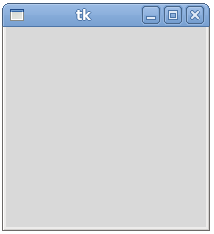
\includegraphics[scale=.5]{../diapos/programas/tkinter/capturas/01.png}

La sentencia \lstinline!w = Tk()! crea la ventana principal del
programa, y la asigna a la variable \lstinline!w!. Toda interfaz gráfica
debe tener una ventana principal en la que se irán agregando cosas. Esta
línea va al principio del programa.

La sentencia \lstinline!w.mainloop()! indica a la interfaz que debe
quedarse esperando a que el usuario haga algo. Esta línea siempre debe
ir al final del programa.

Al ejecutarlo, puede darse cuenta que el programa no termina. Esto
ocurre porque la llamada al método \lstinline!mainloop()! se «queda
pegada» esperando que algo ocurra. Esto se llama un \textbf{ciclo de
eventos}, y es simplemente un ciclo infinito que está continuamente
esperando que algo ocurra.

Todos los programas con interfaz gráfica deben seguir esta estructura:
la creación de la ventana al principio del programa y la llamada al
ciclo de eventos al final del programa.

\section{Creación de widgets}

Un \textbf{widget} es cualquier cosa que uno puede poner en una ventana.
Por ahora, veremos tres tipos de widgets sencillos, que son suficientes
para crear una interfaz gráfica funcional:

\begin{itemize}
\item
  las \textbf{etiquetas} (\lstinline!Label!) sirven para mostrar datos,
\item
  los \textbf{botones} (\lstinline!Button!) sirven para hacer que algo
  ocurra en el programa, y
\item
  los \textbf{campos de entrada} (\lstinline!Entry!) sirven para
  ingresar datos al programa.
\end{itemize}

En un programa en ejecución, estos widgets se ven así:

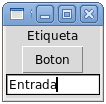
\includegraphics{../diapos/programas/tkinter/capturas/widgets.png}

El \lstinline!Entry! es análogo al \lstinline!raw_input! de los
programas de consola: sirve para que el programa reciba la entrada. El
\lstinline!Label! es análogo al \lstinline!print!: sirve para que el
programa entregue la salida.

Un botón puede ser visto como un «llamador de funciones»: cada vez que
un botón es presionado, se hace una llamada a la función asociada a ese
botón. Los botones no tienen un análogo, pues los programas de consola
se ejecutan de principio a fin inmediatamente, y por esto no necesitan
que las llamadas a las funciones sean gatilladas por el usuario.

Para agregar un widget a un programa, hay que ocupar las funciones con
los nombres de los widgets (\lstinline!Label!, \lstinline!Button! y
\lstinline!Entry!). Estas funciones reciben como primer parámetro
obligatorio la ventana que contendrá el widget. Además, tienen
parámetros opcionales que deben ser pasados usando la sintaxis de
asignación de parámetros por nombre. Por ejemplo, el parámetro
\lstinline!text! sirve para indicar cuál es el texto que aparecerá en un
botón o en una etiqueta.

Por ejemplo, la siguiente sentencia crea un botón con el texto
\lstinline!Saludar!, contenido en la ventana \lstinline!w!:

\begin{lstlisting}
b = Button(w, text='Saludar')
\end{lstlisting}

Si bien esto crea el botón y lo asigna a la variable \lstinline!b!, el
botón no es agregado a la ventana \lstinline!w! inmediatamente: lo que
hicimos fue simplemente decirle al botón cuál es su contenedor, para que
lo tenga en cuenta al momento de ser agregado. Para que esto ocurra,
debemos llamar al método \lstinline!pack!, que es una manera de decirle
al widget «empaquétate dentro de tu contenedor»:

\begin{lstlisting}
b.pack()
\end{lstlisting}

Como referencia, el programa que crea la ventana de la imagen es el
si\-guiente (¡pruébelo!):
\begin{lstlisting}
from Tkinter import *

w = Tk()

l = Label(w, text='Etiqueta')
l.pack()

b = Button(w, text='Boton')
b.pack()

e = Entry(w)
e.pack()

w.mainloop()
\end{lstlisting}



Los widgets van siendo apilados verticalmente, desde arriba hacia abajo,
en el mismo orden en que van siendo apilados. Ya veremos cómo
empaquetarlos en otras direcciones.

\section{Controladores}

Al crear un botón de la siguiente manera:
\begin{lstlisting}
b = Button(w, text='Saludar')
\end{lstlisting}
no hay ninguna acción asociada a él. Al hacer clic en el botón, nada
ocurrirá.

Para que ocurra algo al hacer clic en el botón, hay que asociarle una
acción. Un \textbf{controlador} es una función que será ejecutada al
hacer clic en un botón.

Los controladores deben ser funciones que no reciben ningún parámetro.

Por ejemplo, supongamos que queremos que el programa imprima el mensaje
\lstinline!Hola! en la consola cada vez que se haga clic en el botón que
dice «Saludar». Primero, hay que crear el controlador:
\begin{lstlisting}
def saludar():
    print 'Hola'
\end{lstlisting}

Para asociar el controlador al botón, hay que pasarlo a través del
parámetro \lstinline!command! (en inglés: «orden») al momento de crear
el botón:
\begin{lstlisting}
b = Button(w, text='Saludar', command=saludar)
\end{lstlisting}

Esta línea significa: crear el botón \lstinline!b!, contenido en la
ventana \lstinline!w!, que tenga el texto \lstinline!'Saludar'! y que al
hacer clic en él se ejecute la función \lstinline!saludar!.

El siguiente ejemplo es un programa completo que tiene dos botones: uno
para saludar y otro para salir del programa. El controlador del segundo
botón es la función \lstinline!exit!, que ya viene con Python:

\begin{lstlisting}
from Tkinter import *

def saludar():
    print 'Hola'

w = Tk()

l = Label(w, text='Hola progra')
l.pack()

b1 = Button(w, text='Saludar', command=saludar)
b1.pack()

b2 = Button(w, text='Salir', command=exit)
b2.pack()

w.mainloop()
\end{lstlisting}

El programa se ve así:

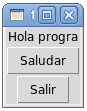
\includegraphics{../diapos/programas/tkinter/capturas/04.png}

Ejecute el programa, y pruebe lo que ocurre al hacer clic en ambos
botones.

\section{Modelos}

Mediante el uso de controladores, ya podemos hacer interfaces que hagan
algo, pero que siguen teniendo una limitación: las interfaces sólo
reaccionan a eventos que ocurren, pero no tienen memoria para recordar
información.

Un \textbf{modelo} es un dato almacenado que está asociado a la
interfaz. Usando modelos, se puede lograr que la interfaz vaya cambiando
su estado interno a medida que ocurren eventos.

En general, a la hora de crear un programa con interfaz gráfica, debemos
crear un modelo para cada dato que deba ser recordado durante el
programa.

Tkinter provee varios tipos de modelos, pero para simplificar podemos
limitarnos a usar sólo modelos de tipo string. Un modelo puede ser
creado de la siguiente manera:

\begin{lstlisting}
m = StringVar()
\end{lstlisting}

Aquí, el modelo \lstinline!m! es capaz de recordar un string

Para modificar el valor del modelo \lstinline!m!, se debe usar el método
\lstinline!set!, que recibe el valor como único parámetro:

\begin{lstlisting}
m.set('hola')
\end{lstlisting}

Para obtener el valor del modelo \lstinline!m!, se debe usar el método
\lstinline!get!, que no recibe ningún parámetro:

\begin{lstlisting}
s = m.get()
\end{lstlisting}

En este ejemplo, la variable \lstinline!s! toma el valor
\lstinline!'hola'!.

Como los modelos creados por \lstinline!StringVar! almacenan datos de
tipo string, hay que tener cuidado de hacer las conversiones apropiadas
si se desea usar datos numéricos:

\begin{lstlisting}
a = StringVar()
b = StringVar()
a.set(5)                # es convertido a string
b.set(8)                # es convertido a string
print a.get() + b.get()             # imprime 58
print int(a.get()) + int(b.get())   # imprime 13
\end{lstlisting}

Usted podría preguntarse cuál es la razón para usar modelos en vez de
usar las variables propias de Python, ---es decir, las que son creadas
mediante asignaciones--- para almacenar los datos. Los modelos tienen la
ventaja que es posible asociarlos a elementos de la interfaz que
responden automáticamente cuando el valor del modelo cambia.

Por ejemplo, podemos asociar una etiqueta a un modelo. La etiqueta
siempre mostrará en la interfaz el valor que tiene el modelo, incluso
cuando éste cambie.
El parámetro \lstinline!textvariable!
asocia el modelo a la etiqueta:

\begin{lstlisting}
x = StringVar()
l = Label(w, textvariable=x)
l.pack()
\end{lstlisting}

Cada vez que cambie el valor del modelo \lstinline!x!, el texto de la
etiqueta será actua\-li\-zado inmediatamente.

También podemos asociar un campo de entrada a un modelo. El valor
asociado al modelo siempre será el texto que está ingresado en el campo.

Para asociar un modelo a un campo de texto, también se usa el parámetro
\lstinline!textvariable!:

\begin{lstlisting}
x = StringVar()
e = Entry(w, textvariable=x)
e.pack()
\end{lstlisting}

Cuando se obtenga el valor del modelo mediante la llamada
\lstinline!x.get()!, el valor retornado será lo que el usuario haya
ingresado en el campo hasta ese momento.

\section{Resumen}

Para diseñar un programa que tiene una interfaz gráfica, hay tres
elementos importantes que hay que tener en consideración.

\begin{enumerate}
\item
  Los elementos que componen la interfaz (la \textbf{vista} del programa).
\item
  Los \textbf{modelos} que mantienen el estado de la interfaz en todo
  momento.
\item
  Los \textbf{controladores} que reaccionan a eventos del usuario.
\end{enumerate}

Los controladores pueden interactuar con los modelos mediante sus
métodos \lstinline!get! y \lstinline[language={}]!set!. Los cambios en los modelos
pueden verse reflejados en la vista.


  \chapter{Expresiones y programas simples}
\section{Evaluación de expresiones}

Sin usar el computador, evalúe las siguientes expresiones, y para cada
una de ellas indique el resultado y su tipo (si la expresión es válida)
o qué error ocurre (si no lo es):

\begin{lstlisting}
>>> 2 + 3      # Respuesta: tipo int, valor 5
>>> 4 / 0      # Respuesta: error de division por cero
>>> 5 + 3 * 2
>>> '5' + '3' * 2
>>> 2 ** 10 == 1000 or 2 ** 7 == 100
>>> int("cuarenta")
>>> 70/16 + 100/24
>>> 200 + 19%
>>> 3 < (1024 % 10) < 6
>>> 'six' + 'eight'
>>> 'six' * 'eight'
>>> float(-int('5') + int('10'))
>>> abs(len('ocho') - len('cinco'))
>>> bool(14) or bool(-20)
>>> float(str(int('5' * 4) / 3)[2])
\end{lstlisting}

Compruebe sus respuestas en el computador.
       % :)
\section{Saludo}

Escriba un programa que pida al usuario que escriba su nombre, y lo
salude llamándolo por su nombre.

\begin{lstlisting}[language=testcase]
Ingrese su nombre: `Perico`
Hola, Perico
\end{lstlisting}
                       % :)
\section{Círculos}

Escriba un programa que reciba como entrada el radio de un círculo y
entregue como salida su perímetro y su área:

\begin{lstlisting}[language=testcase]
Ingrese el radio: `5`
Perimetro: 31.4
Area: 78.5
\end{lstlisting}
                     % :)
\section{Promedio}

Escriba un programa que calcule el promedio de 4 notas ingresadas por el
usuario:
                     % :)
\section{Conversión de unidades de longitud}

Escriba un programa que convierta de centímetros a pulgadas. Una pulgada
es igual a 2.54 centímetros.

\begin{lstlisting}[language=testcase]
Ingrese longitud: `45`
45 cm = 17.7165 in
\end{lstlisting}


\begin{lstlisting}[language=testcase]
Ingrese longitud: `13`
13 cm = 5.1181 in
\end{lstlisting}
 % :)
\section{Número invertido}

Escriba un programa que pida al usuario un entero de tres dígitos, y
entregue el número con los dígitos en orden inverso:
             % :)
%\section{Pitágoras}

Escriba un programa que reciba como entrada las longitudes de los dos
catetos `a` y `b` de un triángulo rectángulo, y que entregue como salida
el largo de la hipotenusa `c` del triangulo, dado por el
\href{http://es.wikipedia.org/wiki/Teorema\_de\_Pit\%C3\%A1goras}{teorema
de Pitágoras}: `c\^{}2 = a\^{}2 + b\^{}2`.

\section{Hora futura}

Escriba un programa que pregunte al usuario la hora actual \emph{t} del
reloj y un número entero de horas \emph{h}, que indique qué hora marcará
el reloj dentro de \emph{h} horas:
                  % :)
\section{Parte decimal}

Escriba un programa que entregue la parte decimal de un número real
ingresado por el usuario.

\begin{lstlisting}[language=testcase]
Ingrese un numero: `4.5`
0.5
\end{lstlisting}

\begin{lstlisting}[language=testcase]
Ingrese un numero: `-1.19`
0.19
\end{lstlisting}



%\section{Qué nota necesito}

Un alumno desea saber que nota necesita en el tercer certamen para
aprobar un ramo.

El promedio del ramo se calcula con la siguiente formula.

\[N_C = \frac{(C1+C2+C3)}{3}\]\[N_F = N_C\cdot 0.7 + N_L\cdot 0.3\]

Donde `N\_C` es el promedio de certámenes, `N\_L` el promedio de
laboratorio y `N\_F` la nota final.

Escriba un programa que pregunte al usuario las notas de los dos
primeros certamen y la nota de laboratorio, y muestre la nota que
necesita el alumno para aprobar el ramo con nota final 60.

%\section{Huevos a la copa}

\emph{Ejercicio sacado de} {[}Lang09{]}\_.

Cuando un huevo es hervido en agua, las proteínas comienzan a coagularse
cuando la temperatura sobrepasa un punto crítico. A medida que la
temperatura aumenta, las reacciones se aceleran.

En la clara, las proteínas comienzan a coagularse para temperaturas
sobre 63°C, mientras que en la yema lo hacen para temperaturas sobre
70°C. Para hacer un huevo a la copa, la clara debe haber sido calentada
lo suficiente para coagularse a más de 63°C, pero la yema no debe
sobrepasar los 70°C para evitar obtener un huevo duro.

El tiempo en segundos que toma al centro de la yema alcanzar `T\_y` °C
está dado por la fórmula:

\[t = \frac{M^{2/3} c \rho^{1/3}}
{K\pi^2(4\pi/3)^{2/3}}
\ln\left[
0.76\frac{T_o - T_w}
{T_y - T_w}
\right],\]

donde `M` es la masa del huevo, `rho` su densidad, `c` su capacidad
calorífica específica y `K` su conductividad térmica. Algunos valores
típicos son:

\begin{itemize}
\item
  `M = 47,{[}text\{g\}{]}` para un huevo pequeño y `M =
  67,{[}text\{g\}{]}` para uno grande,
\item
  `rho = 1.038,{[}text\{g\},text\{cm\}\^{}\{-3\}{]}`,
\item
  `c = 3.7,{[}text\{J\},text\{g\}\^{}\{-1\} text\{K\}\^{}\{-1\}{]}`, y
\item
  `K = 5.4cdot 10\^{}\{-3\},{[}text\{W\},text\{cm\}\^{}\{-1\}
  text\{K\}\^{}\{-1\}`{]}.
\end{itemize}

`T\_w` es la temperatura de ebullición del agua y `T\_o` la temperatura
original del huevo antes de meterlo al agua, ambos en grados Celsius.

Escriba un programa que reciba como entrada la temperatura original del
huevo y muestre como salida el tiempo en segundos que le toma alcanzar
la temperatura máxima para prepararlo a la copa.


\chapter{Estructuras condicionales}
\section{Determinar par}

Escriba un programa que determine si el número entero ingresado por el
usuario es par o no.
                  % :)
\section{Años bisiestos}

Cuando la Tierra completa una órbita alrededor del Sol, no han
transcurrido exactamente 365 rotaciones sobre sí misma, sino un poco
más. Más precisamente, la diferencia es de más o menos un cuarto de día.

Para evitar que las estaciones se desfasen con el calendario, el
calendario juliano introdujo la regla de introducir un día adicional en
los años divisibles por 4 (llamados
\href{http://es.wikipedia.org/wiki/A\%C3\%B1o\_bisiesto}{bisiestos}),
para tomar en consideración los cuatro cuartos de día acumulados.

Sin embargo, bajo esta regla sigue habiendo un desfase, que es de
aproximadamente \(3/400\) de día.

Para corregir este desfase, en el año 1582 el papa Gregorio XIII
introdujo un nuevo calendario, en el que el último año de cada siglo
dejaba de ser bisiesto, a no ser que fuera divisible por 400.

Escriba un programa que indique si un año es bisiesto o no, teniendo en
cuenta cuál era el calendario vigente en ese año:

\begin{lstlisting}[language=testcase]
Ingrese un anno: `1988`
1988 es bisiesto
\end{lstlisting}

\begin{lstlisting}[language=testcase]
Ingrese un anno: `2011`
2011 no es bisiesto
\end{lstlisting}

\begin{lstlisting}[language=testcase]
Ingrese un anno: `1700`
1700 no es bisiesto
\end{lstlisting}

\begin{lstlisting}[language=testcase]
Ingrese un anno: `1500`
1500 es bisiesto
\end{lstlisting}

\begin{lstlisting}[language=testcase]
Ingrese un anno: `2400`
2400 es bisiesto
\end{lstlisting}

                    % :)
%\section{División}

Escriba un programa que pida dos números enteros y que calcule la
división, indicando si la división es exacta o no.

\section{Palabra más larga}

Escriba un programa que pida al usuario dos palabras, y que indique cuál
de ellas es la más larga y por cuántas letras lo es.

\begin{lstlisting}[language=testcase]
Palabra 1: `edificio`
Palabra 2: `tren`
La palabra edificio tiene 4 letras mas que tren.
\end{lstlisting}

\begin{lstlisting}[language=testcase]
Palabra 1: `sol`
Palabra 2: `paralelepipedo`
La palabra paralelepipedo tiene 11 letras mas que sol
\end{lstlisting}

\begin{lstlisting}[language=testcase]
Palabra 1: `plancha`
Palabra 2: `lapices`
Las dos palabras tienen el mismo largo
\end{lstlisting}


            % :)
\section{Ordenamiento}

Escriba un programa que reciba como entrada dos números, y los muestre
ordenados de menor a mayor:

\begin{lstlisting}[language=testcase]
Ingrese numero: `51`
Ingrese numero: `24`
24 51
\end{lstlisting}

A continuación, escriba otro programa que haga lo mismo con tres
números:

\begin{lstlisting}[language=testcase]
Ingrese numero: `8`
Ingrese numero: `1`
Ingrese numero: `4`
1 4 8
\end{lstlisting}

Finalmente, escriba un tercer programa que ordene cuatro números:

\begin{lstlisting}[language=testcase]
Ingrese numero: `7`
Ingrese numero: `0`
Ingrese numero: `6`
Ingrese numero: `1`
0 1 6 7
\end{lstlisting}

Recuerde que su programa debe entregar la solución correcta para
cualquier combinación de números, no sólo para los ejemplos mostrados
aquí.

Hay más de una manera de resolver cada ejercicio.
          % :)
%\section{Letra o número}

Escriba un programa que determine si un caracter ingresado es letra,
número, o ninguno de los dos. En caso que sea letra, determine si es
mayúscula o minúscula.

%\chapter{Calculadora simple}

El siguiente programa es una calculadora simple:

Al ejecutar el programa, primero uno ingresa la operación que será
aplicada, que puede ser:

\ctable[pos = H, center, botcap]{ll}
{% notes
}
{% rows
\FL
Signo & Operación
\\\noalign{\medskip}
------- & ---------------
\\\noalign{\medskip}
\lstinline!+! & Suma
\\\noalign{\medskip}
\lstinline!-! & Resta
\\\noalign{\medskip}
\lstinline!*! & Multiplicación
\\\noalign{\medskip}
\lstinline!/! & División
\\\noalign{\medskip}
\lstinline!^! & Potencia
\LL
}

La multiplicación también puede ser indicada con una \lstinline!x!
minúscula.

A continuación, se debe ingresar los dos operandos. Finalmente, el
programa muestra el resultado de la operación.

Escriba, compile y ejecute este programa.

En este programa puede ver que es posible asignar un valor inicial a una
variable al momento de declararla:

\begin{lstlisting}
float resultado = 1.0;
int valido = 1;
\end{lstlisting}

También note que tanto en el \lstinline!if! como en el \lstinline!else!
del final se ha omitido los paréntesis de llave (\lstinline!{}!) ya que
en ambos casos hay incluída solamente una única sentencia.

\section{Definición de funciones}

Al principio del programa, se ha definido una función llamada
\lstinline!potencia!. Ella recibe como parámetros la base (un número
real) y el exponente (un entero), y retorna el resultado de elevar la
base al exponente.

En C no existe un operador «elevado a» (como el \lstinline!**! de
Python), por lo que sí es útil definir una función como ésta.

Es necesario especificar explícitamente cuál será el tipo del valor
retornado (en este caso \lstinline!float!) y los tipos de cada uno de
los parámetros (en el ejemplo, \lstinline!float! e \lstinline!int!).

Las variables declaradas dentro de la función se llaman
\textbf{variables locales}. Estas variables comienzan a existir al
momento de llamar a la función, y desaparecen cuando la función termina.
Son invisibles desde fuera de la función.

En nuestro programa, las dos funciones \lstinline!main! y
\lstinline!potencia! tienen una variable local llamada
\lstinline!resultado!. Ambas variables son distintas, y sus valores
respectivos están almacenados en regiones diferentes de la memoria.

\section{Tipo char}

El tipo \lstinline!char! se usa para representar caracteres (símbolos)
solitarios. La variable \lstinline!op! que almacena la operación es de
este tipo.

Un valor de tipo \lstinline!char! se representa en un programa entre
comillas simples. Por ejemplo, el signo más está representado como
\lstinline!'+'!.

Técnicamente, los valores de tipo \lstinline!char! son números enteros
que están comprendidos entre −128 y 127. Cada número está asociado a un
caracter a través de la
\href{http://es.wikipedia.org/wiki/C\%C3\%B3digo\_ASCII\#Caracteres\_imprimibles\_ASCII}{tabla
ASCII}. Los enteros y los caracteres asociados son intercambiables; por
ejemplo, la expresión \lstinline!'m' == 109! es evaluada como verdadera.

No hay que confundir un caracter con un string de largo uno:
\lstinline!'a'! y \lstinline!"a"! son dos cosas distintas.

\section{Sentencia switch}

El \textbf{switch} es una sentencia de control condicional que permite
indicar qué hacer si el resultado de una expresión es igual a alguno de
ciertos valores constantes indicados

Un ejemplo de uso de \lstinline!switch! es el siguiente:

\begin{lstlisting}
switch (expresion) {
    case 1:
        /* que hacer cuando expresion == 1 */

    case 2:
        /* que hacer cuando expresion == 2 */

    default:
        /* que hacer cuando la expresion no es igual
         * a ninguno de los casos anteriores */
}
\end{lstlisting}

Cuando el resultado de la expresión es igual a alguno de los valores
indicados, la ejecución del programa salta al \lstinline!case! con ese
valor. Si el valor con el resultado no existe, salta a
\lstinline!default!.

Hay que tener cuidado con una característica extraña del
\lstinline!switch!: cuando se cumple un caso, los casos que vienen a
continuación también se ejecutan. En este ejemplo:

\begin{itemize}
\item
  si \lstinline!expresion == 1!, el programa saltará a
  \lstinline!case 1!, y luego continuará con \lstinline!case 2! y
  \lstinline!default!;
\item
  si \lstinline!expresion == 2!, el programa saltará a
  \lstinline!case 2!, y luego continuará con \lstinline!default!;
\item
  si \lstinline!expresion! no es ni 1 ni 2, el programa saltará a
  \lstinline!default!.
\end{itemize}

Para evitar que los casos siguientes sean ejecutados, debe ponerse un
\lstinline!break! al final de cada caso. Esto es lo que se hizo en el
programa de la calculadora.

\section{Conversión de tipos}

El segundo parámetro de la función \lstinline!potencia! es entero, pero
los operandos ingresados por el usuario son almacenados como números
reales.

Para convertir el exponente de real a entero, basta con anteponer al
valor el tipo entre paréntesis.

En este caso particular, la conversión se hace truncando los decimales
del número real. Así, si \lstinline!y! vale \lstinline!5.9!, entonces
\lstinline!(int) y! vale \lstinline!5!. Para conversiones entre otros
tipos, se siguen otras reglas diferentes.

En inglés, el nombre de esta operación es \emph{cast}. Posiblemente
usted escuche más de una vez a alguien refiriéndose a esta operación
como «castear».

\section{Ejercicios}

Modifique el programa de modo que soporte una nueva operación: obtener
el \href{http://es.wikipedia.org/wiki/Coeficiente\_binomial}{coeficiente
binomial} entre \lstinline!x! e \lstinline!y!. Esta operación debe ser
indicada con el símbolo \lstinline!b!:

El coeficiente binomial es una operación entre números enteros. Tenga
cuidado y use conversiones apropiadas.

\chapter{Calcular la edad del usuario}

El siguiente programa le pide al usuario ingresar su año de nacimiento y
el año actual. A continuación, le muestra cuál es su edad:

Como siempre, el código del programa debe estar incluído dentro de una
función llamada \lstinline!main!, y la última sentencia del programa
debe ser \lstinline!return 0!.

Escriba, compile y ejecute este programa.

\section{Declaración de variables}

Este programa utiliza tres variables, llamadas \lstinline!nacimiento!,
\lstinline!actual! y \lstinline!edad!.

En Python, las variables eran creadas automáticamente al momento de
asignarlas por primera vez:

\begin{lstlisting}
nacimiento = int(raw_input("Ingrese su anno de nacimiento: "))
actual = int(raw_input("Ingrese el anno actual: "))
edad = actual - nacimiento
\end{lstlisting}

En C no es así. Las variables deben ser \textbf{declaradas} antes de ser
usadas. Además, uno debe indicar de qué tipo serán los datos que se
almacenarán en cada variable. Una variable sólo puede almacenar valores
de un único tipo.

Las tres primeras sentencias del programa declaran las variables
\lstinline!nacimiento!, \lstinline!actual! y \lstinline!edad! para
almacenar valores de tipo \lstinline!int! (entero).

En C, todas las declaraciones deben cumplir con esta sintaxis:

\begin{lstlisting}
tipo variable;
\end{lstlisting}

\subsubsection{¿Por qué es necesario declarar las variables?}

Una característica del lenguaje C es que entrega al programador el poder
(y la responsabilidad) de decidir muy de cerca cómo usar la memoria del
computador. En Python, al contrario, el intérprete decide por uno
cuándo, cómo y cuánta memoria el programa utilizará, lo que es muy
conveniente a la hora de programar pero que puede conducir a un uso
ineficiente de los recursos disponibles en ciertas ocasiones.

En nuestro programa de ejemplo, el compilador analizará el código y
sabrá que el programa sólo almacenará tres valores, y que cada uno sólo
necesitará el espacio suficiente para guardar un número entero. ¡Todo
esto ocurre antes de que el programa sea siquiera ejecutado por primera
vez!

\section{Entrada con formato usando scanf}

Ya conocimos la función \lstinline!printf!, que sirve para imprimir un
(único) string por pantalla.

Para recibir la entrada del programa se utiliza la función
\textbf{scanf}, cuyo uso puede parecer un poco extraño al principio.

El primer parámetro de la función \lstinline!scanf! es un string que
describe cuál es el formato en el que estará representado el valor a
ingresar. En este ejemplo, el string \lstinline!"%d"! indica que el
valor que será leído debe ser interpretado como un número entero en
representación decimal (dígitos del 0 al 9, posiblemente con un signo al
principio). Por supuesto, hay muchos otros descriptores de formato.

El segundo parámetro debe indicar \textbf{en qué lugar de la memoria del
computador se debe guardar el valor ingresado}. Note que aquí no se pone
la variable a secas, sino que antecedida de un signo \lstinline!&!. La
distinción es importante:

\begin{itemize}
\item
  \lstinline!nacimiento! es el valor que tiene la variable
  \lstinline!nacimiento!,
\item
  \lstinline!&nacimiento! es la ubicación en la memoria de la variable
  \lstinline!nacimiento!.
\end{itemize}

El operador \lstinline!&! se lee como «la dirección de». Más adelante
veremos qué significa esto.

En resumen, la sentencia:

\begin{lstlisting}
scanf("%d", &nacimiento);
\end{lstlisting}

es equivalente a la siguiente sentencia en Python:

\begin{lstlisting}
nacimiento = int(raw_input())
\end{lstlisting}

\section{Salida con formato usando printf}

La función \lstinline!printf! imprime sólo strings, no enteros. Sin
embargo, es posible insertar enteros dentro del mensaje usando
descriptores de formato idénticos a los de la función \lstinline!scanf!.

En las posiciones del string en las que se desea mostrar un número
entero, debe insertarse el texto \lstinline!%d!. Luego, cada uno de los
valores enteros por imprimir deben ser pasados como parámetros
adicionales a la función.

Los siguientes ejemplos muestran usos correctos e incorrectos de
\lstinline!printf!. Haga el ejercicio de darse cuenta de los errores:

\begin{lstlisting}
/* Correctos */
printf("Hola mundo\n");
printf("Usted tiene %d annos.", edad);
printf("Usted tiene %d annos.\n", edad);
printf("Usted tiene 18 annos.");
printf("Usted tiene %d annos.", 18);
printf("Usted tiene %d annos y %d meses.", edad, meses);

/* Incorrectos */
printf("Usted tiene %d annos.");
printf("Usted tiene annos.", edad);
printf("Usted tiene annos.", 18);
printf("Usted tiene", edad, "annos.");
printf("Usted tiene edad annos.");
printf("Usted tiene"); printf(edad); printf("annos.");
printf("Usted tiene %d annos y %d meses.", edad);
\end{lstlisting}

\section{Ejercicio}

Escriba un programa que pregunte al usuario las notas de sus cuatro
certámenes, y le muestre cuál es su promedio, con decimales:

Para declarar una variable de tipo real, se debe indicar que el tipo es
\lstinline!float!.

Para leer y para mostrar un número real con decimales, se usa el
descriptor de formato \lstinline!%f!.
                         % :)
\section{Set de tenis}

El joven periodista Solarrabietas debe relatar un partido de tenis, pero
no conoce las reglas del deporte. En particular, no ha logrado aprender
cómo saber si un set ya terminó, y quién lo ganó.

Un partido de tenis se divide en sets. Para ganar un set, un jugador
debe ganar 6 juegos, pero además debe haber ganado por lo menos dos
juegos más que su rival. Si el set está empatado a 5 juegos, el ganador
es el primero que llegue a 7. Si el set está empatado a 6 juegos, el set
se define en un último juego, en cuyo caso el resultado final es 7-6.

Sabiendo que el jugador A ha ganado \emph{m} juegos, y el jugador B,
\emph{n} juegos, al periodista le gustaría saber:

\begin{itemize}
\item
  si A ganó el set, o
\item
  si B ganó el set, o
\item
  si el set todavía no termina, o
\item
  si el resultado es inválido (por ejemplo, 8-6 o 7-3).
\end{itemize}

Desarrolle un programa que solucione el problema de Solarrabietas:

\begin{lstlisting}[language=testcase]
Juegos ganados por A: `4`
Juegos ganados por B: `5`
Aun no termina
\end{lstlisting}

\begin{lstlisting}[language=testcase]
Juegos ganados por A: `5`
Juegos ganados por B: `7`
Gano B
\end{lstlisting}

\begin{lstlisting}[language=testcase]
Juegos ganados por A: `5`
Juegos ganados por B: `6`
Aun no termina
\end{lstlisting}

\begin{lstlisting}[language=testcase]
Juegos ganados por A: `3`
Juegos ganados por B: `7`
Invalido
\end{lstlisting}

\begin{lstlisting}[language=testcase]
Juegos ganados por A: `6`
Juegos ganados por B: `4`
Gano A
\end{lstlisting}

                 % :)
\section{Triángulos}

Los tres lados \emph{a}, \emph{b} y \emph{c} de un triángulo deben
satisfacer la
\href{http://es.wikipedia.org/wiki/Desigualdad\_triangular}{desigualdad
triangular}: cada uno de los lados no puede ser más largo que la suma de
los otros dos.

Escriba un programa que reciba como entrada los tres lados de un
triángulo, e indique:

\begin{itemize}
\item
  si acaso el triángulo es inválido; y
\item
  si no lo es, qué tipo de triángulo es.
\end{itemize}
                   % :)
%\section{Índice de masa corporal}

\emph{Ejercicio sacado de} {[}Camp09{]}\_.

El riesgo de que una persona sufra enfermedades coronarias depende de su
edad y su índice de masa corporal:

\begin{quote}
\ctable[pos = H, center, botcap]{lll}
{% notes
}
{% rows
\FL
\parbox[b]{0.24\columnwidth}{\raggedright
} & \parbox[b]{0.22\columnwidth}{\raggedright
edad \textless{} 45
} & \parbox[b]{0.22\columnwidth}{\raggedright
edad ≥ 45
}
\ML
\parbox[t]{0.24\columnwidth}{\raggedright
\textbf{IMC \textless{} 22.0}
} & \parbox[t]{0.22\columnwidth}{\raggedright
bajo
} & \parbox[t]{0.22\columnwidth}{\raggedright
medio
}
\\\noalign{\medskip}
\parbox[t]{0.24\columnwidth}{\raggedright
\textbf{IMC ≥ 22.0}
} & \parbox[t]{0.22\columnwidth}{\raggedright
medio
} & \parbox[t]{0.22\columnwidth}{\raggedright
alto
}
\LL
}
\end{quote}

El índice de masa corporal es el cuociente entre el peso del individuo
en kilos y el cuadrado de su estatura en metros.

Escriba un programa que reciba como entrada la estatura, el peso y la
edad de una persona, y le entregue su condición de riesgo.


\chapter{Ciclos}
\section{Múltiplos}

Escriba un programa que muestre la tabla de multiplicar del 1 al 10 del
número ingresado por el usuario:

\begin{lstlisting}[language=testcase]
Ingrese un numero: `9`
9 x 1 = 9
9 x 2 = 18
9 x 3 = 27
9 x 4 = 36
9 x 5 = 45
9 x 6 = 54
9 x 7 = 63
9 x 8 = 72
9 x 9 = 81
9 x 10 = 90
\end{lstlisting}
                    % :)
\section{Potencias de dos}

Escriba un programa que genere todas las potencias de 2, desde la
0-ésima hasta la ingresada por el usuario:

\begin{lstlisting}[language=testcase]
Ingrese num: `10`
1 2 4 8 16 32 64 128 256 512 1024
\end{lstlisting}

                % :)
%\section{Suma entre números}

Escriba un programa que pida al usuario dos números enteros, y luego
entregue la suma de todos los números que están entre ellos. Por
ejemplo, si los números son 1 y 7, debe entregar como resultado 2 + 3 +
4 + 5 + 6 = 20.

\section{Divisores}

Escriba un programa que entregue todos los divisores del número entero
ingresado:

\begin{lstlisting}[language=testcase]
Ingrese numero: `200`
1 2 4 5 8 10 20 25 40 50 100 200
\end{lstlisting}
                    % :)
\section{Tabla de multiplicar}

Escriba un programa que muestre una tabla de multiplicar como la
siguiente.
Los números deben estar alineados a la derecha.
\begin{lstlisting}[language=testcase]
 1   2   3   4   5   6   7   8   9  10
 2   4   6   8  10  12  14  16  18  20
 3   6   9  12  15  18  21  24  27  30
 4   8  12  16  20  24  28  32  36  40
 5  10  15  20  25  30  35  40  45  50
 6  12  18  24  30  36  42  48  54  60
 7  14  21  28  35  42  49  56  63  70
 8  16  24  32  40  48  56  64  72  80
 9  18  27  36  45  54  63  72  81  90
10  20  30  40  50  60  70  80  90 100
\end{lstlisting}

        % :)
\section{Tiempo de viaje}

Un viajero desea saber cuánto tiempo tomó un viaje que realizó. Él tiene
la duración en minutos de cada uno de los tramos del viaje.

Desarrolle un programa que permita ingresar los tiempos de viaje de los
tramos y entregue como resultado el tiempo total de viaje en formato
\lstinline!horas:minutos!.
El programa debe dejar de pedir tiempos de viaje cuando se ingresa un 0.

\begin{lstlisting}[language=testcase]
Duracion tramo: `15`
Duracion tramo: `30`
Duracion tramo: `87`
Duracion tramo: `0`
Tiempo total de viaje: 2:12 horas
\end{lstlisting}

\begin{lstlisting}[language=testcase]
Duracion tramo: `51`
Duracion tramo: `17`
Duracion tramo: `0`
Tiempo total de viaje: 1:08 horas
\end{lstlisting}

              % :)
\section{Dibujos de asteriscos}

\begin{enumerate}
\item
  Escriba un programa que pida al usuario ingresar la altura y el ancho
  de un rectángulo y lo dibuje utilizando asteriscos:
\item
  Escriba un programa que dibuje el triángulo del tamaño indicado por el
  usuario de acuerdo al ejemplo:
\item
  Escriba un programa que dibuje el hexágono del tamaño indicado por el
  usuario de acuerdo al ejemplo:
\end{enumerate}
           % :)
\section{$\pi$}

Desarolle un programa para estimar el valor de
\href{http://es.wikipedia.org/wiki/N\%C3\%BAmero\_\%CF\%80}{\(\pi\)} usando la
siguiente suma infinita:

\[\pi = 4 \left(1-\frac{1}{3}+\frac{1}{5}-\frac{1}{7}+ \cdots \right)\]

La entrada del programa debe ser un número entero \(n\) que indique
cuántos términos de la suma se utilizará.

\begin{lstlisting}[language=testcase]
n: `3`
3.466666666666667
\end{lstlisting}

\begin{lstlisting}[language=testcase]
n: `1000`
3.140592653839794
\end{lstlisting}
                           % :)
%\section{Suma de fracciones}

Desarrolle un programa que permita trabajar con las potencias
fraccionales de dos, es decir:

\[\frac{1}{2}, \frac{1}{4}, \frac{1}{8}, \frac{1}{16}, \frac{1}{32}, \frac{1}{64}, \ldots\]

en forma decimal:

\[0.5, 0.25, 0.125, 0.0625, 0.03125, 0.015625, \ldots\]

El programa debe mostrar tres columnas que contengan la siguiente
información:

\begin{lstlisting}
Potencia  Fraccion  Suma
1         0.5       0.5
2         0.25      0.75
3         0.125     0.875
4         0.0625    0.9375
...       ...       ...
\end{lstlisting}

El programa debe terminar cuando la fracción decimal sea menor o igual a
0.000001.

\section{$e$}

El número de Euler, \(e\approx 2,71828\), puede ser representado como la
siguiente suma infinita:

\[e = \frac{1}{0!} +  \frac{1}{1!} +  \frac{1}{2!} +  \frac{1}{3!} +  \frac{1}{4!} + \cdots\]

Desarrolle un programa que entregue un valor aproximado de \(e\),
calculando esta suma hasta que la diferencia entre dos sumandos
consecutivos sea menor que \(0.0001\).

Recuerde que el factorial \(n!\) es el producto de los números de \(1\) a
\(n\).
                            % :)
\section{Secuencia de Collatz}

La secuencia de Collatz de un número entero se construye de la siguiente
forma:

\begin{itemize}
\item
  si el número es par, se lo divide por dos;
\item
  si es impar, se le multiplica tres y se le suma uno;
\item
  la sucesión termina al llegar a uno.
\end{itemize}

La \href{http://es.wikipedia.org/wiki/Conjetura\_de\_Collatz}{conjetura
de Collatz} afirma que, al partir desde cualquier número, la secuencia
siempre llegará a 1. A pesar de ser una afirmación a simple vista muy
simple, no se ha podido demostrar si es cierta o no.

Usando computadores, se ha verificado que la sucesión efectivamente
llega a 1 partiendo desde cualquier número natural menor que
`2\^{}\{58\}`.

\begin{enumerate}
\item
  Desarrolle un programa que entregue la secuencia de Collatz de un
  número entero:
\item
  Desarrolle un programa que grafique los largos de las secuencias de
  Collatz de los números enteros positivos menores que el ingresado por
  el usuario:
\end{enumerate}
                      % :)

\chapter{Patrones comunes}
%\section{No múltiplos}

Escriba un programa que muestre los números naturales menores o iguales
que un número \emph{n} determinado, que no sean múltiplos ni de 3 ni de
7.

%\section{Suma de naturales}

Escriba un programa que entregue la suma de los primeros `n` números
naturales, siendo `n` ingresado por el usuario.

Matemáticamente lo que se pide que haga el programa es realizar la
siguiente sumatoria.

\[S_1 = \sum_{i=1}^{n} i = 1+2+3+4+5+6+\cdots+n\]

Además, obtenga el resultado de la siguiente fórmula.

\[S_2 \frac{n\times(n+1)}{2}\]

El programa debe entregar el resultado diciendo si `S\_1` y `S\_2` son
iguales o no.

\section{Número mayor}

Escriba un programa que permita determinar el número mayor perteneciente
a un conjunto de \emph{n} números, donde tanto el valor de \emph{n} como
el de los números deben ser ingresados por el usuario.
                 % :)
\chapter{Productos entre arreglos}

Recordemos que \textbf{vector} es sinónimo de arreglo de una dimensión,
y \textbf{matriz} es sinónimo de arreglo de dos dimensiones.

\section{Producto interno (vector-vector)}

El \textbf{producto interno} entre dos vectores es la suma de los
productos entre elementos correspondientes:

\includegraphics{../diagramas/producto-interno.png}

El producto interno entre dos vectores se obtiene usando la función
\lstinline!dot! provista por NumPy:

\begin{lstlisting}
>>> a = array([-2.8 , -0.88,  2.76,  1.3 ,  4.43])
>>> b = array([ 0.25, -1.58,  1.32, -0.34, -4.22])
>>> dot(a, b)
-14.803
\end{lstlisting}

El producto interno es una operación muy común. Por ejemplo, suele
usarse para calcular totales:

\begin{lstlisting}
>>> precios = array([200, 100, 500, 400, 400, 150])
>>> cantidades = array([1, 0, 0, 2, 1, 0])
>>> total_a_pagar = dot(precios, cantidades)
>>> total_a_pagar
1400
\end{lstlisting}

También se usa para calcular promedios ponderados:

\begin{lstlisting}
>>> notas = array([45, 98, 32])
>>> ponderaciones = array([30, 30, 40]) / 100.
>>> nota_final = dot(notas, ponderaciones)
>>> nota_final
55.7
\end{lstlisting}

\section{Producto matriz-vector}

El \textbf{producto matriz-vector} es el vector de los productos
internos El producto matriz-vector puede ser visto simplemente como
varios productos internos calculados de una sola vez.

Esta operación también es obtenida usando la función \lstinline!dot!
entre las filas de la matriz y el vector:

\includegraphics{../diagramas/matriz-vector.png}

El producto matriz-vector puede ser visto simplemente como varios
productos internos calculados de una sola vez.

Esta operación también es obtenida usando la función \lstinline!dot!:

\begin{lstlisting}
>>> a = array([[-0.6,  4.8, -1.2],
               [-2. , -3.6, -2.1],
               [ 1.7,  4.9,  0. ]])
>>> x = array([-0.6, -2. ,  1.7])
>>> dot(a, x)
array([-11.28,   4.83, -10.82])
\end{lstlisting}

\section{Producto matriz-matriz}

El \textbf{producto matriz-matriz} es la matriz de los productos
internos entre las filas de la primera matriz y las columnas de la
segunda:

\includegraphics{../diagramas/matriz-matriz.png}

Esta operación también es obtenida usando la función \lstinline!dot!:

\begin{lstlisting}
>>> a = array([[ 2,  8],
               [-3,  7],
               [-8, -5]])
>>> b array([[-3, -5, -6, -3],
             [-9, -2,  3, -3]])
>>> dot(a, b)
array([[-78, -26,  12, -30],
       [-54,   1,  39, -12],
       [ 69,  50,  33,  39]])
\end{lstlisting}

La multiplicación de matrices puede ser vista como varios productos
matriz-vector (usando como vectores todas las filas de la segunda
matriz), calculados de una sola vez.

En resumen, al usar la función \lstinline!dot!, la estructura del
resultado depende de cuáles son los parámetros pasados:

\begin{lstlisting}
dot(vector, vector) → número
dot(matriz, vector) → vector
dot(matriz, matriz) → matriz
\end{lstlisting}

                    % :)
\section{Contar combinaciones de dados}

Un jugador debe lanzar dos dados numerados de 1 a 6, y su puntaje es la
suma de los valores obtenidos.

Un puntaje dado puede ser obtenido con varias combinaciones posibles.
Por ejemplo, el puntaje 4 se logra con las siguientes tres
combinaciones: \(1+3\), \(2+2\) y \(3+1\).

Escriba un programa que pregunte al usuario un puntaje,
y muestre como resultado la cantidad de combinaciones de dados
con las que se puede obtener ese puntaje.

\begin{lstlisting}[language=testcase]
Ingrese el puntaje: `4`
Hay 3 combinaciones para obtener 4
\end{lstlisting}

\begin{lstlisting}[language=testcase]
Ingrese el puntaje: `11`
Hay 2 combinaciones para obtener 11
\end{lstlisting}

\begin{lstlisting}[language=testcase]
Ingrese el puntaje: `17`
Hay 0 combinaciones para obtener 17
\end{lstlisting}

   % :)
\section{Histograma}

Escriba un programa que pida al usuario que ingrese varios valores
enteros, que pueden ser positivos o negativos. Cuando se ingrese un
cero, el programa debe terminar y mostrar un gráfico de cuántos valores
positivos y negativos fueron ingresados:
                   % :)
\section{Más corta y más larga}

Desarrolle un programa que tenga la siguiente entrada:

\begin{itemize}
\item
  primero, el usuario ingresa un número entero \emph{n}, que indica
  cuántas palabras ingresará a continuación;
\item
  después el usuario ingresa \emph{n} palabras.
\end{itemize}

La salida del programa debe mostrar la palabra más larga y la más corta
que fueron ingresadas por el usuario.

Recuerde que la función \lstinline!len! entrega el largo de un string:

\begin{lstlisting}
>>> len('amarillo')
8
\end{lstlisting}

La ejecución del programa debe verse así:
                  % :)
\section{Piezas de dominó}

Desarrolle un programa que permita determinar la cantidad total de
puntos que contiene un juego de dominó de 28 piezas.

A modo de ejemplo, considere la pieza de la siguiente figura,
que tiene 5 puntos:

\documentclass{minimal}
\usepackage[pdftex,active,tightpage]{preview}
\usepackage[utf8]{inputenc}
\usepackage[spanish]{babel}
\usepackage{tikz}
%\usetikzlibrary{calc,shapes,arrows}

\begin{document}
%\input{flujo}
\begin{preview}
\begin{tikzpicture}
   [place/.style={circle,draw,fill=black,inner sep=0pt,thick,minimum size=2mm}]
   \def\rectanglepath{-- ++(1cm,0cm)-- ++(0cm,1cm)-- ++(-1cm,0cm) -- cycle}
   \draw (0,0) \rectanglepath;
   \draw (1,0) \rectanglepath;
   \node at (0.5,0.5) [place] {};
   \node at (1.25,0.75) [place] {};
   \node at (1.25,0.25) [place] {};
   \node at (1.75,0.75) [place] {};
   \node at (1.75,0.25) [place] {};
\end{tikzpicture}
\end{preview}
\end{document}


Además, recuerde que en el dominó cada lado de una pieza toma valores
entre 0 y 6 y que, por ejemplo, la pieza cuyos lados toman valores 1 y 4
es la misma que la pieza con valores 4 y 1.
                % :)
%\section{Lanzar dados}

Escriba un programa que muestre todas las combinaciones posibles al
momento de lanzar dos dados de 6 caras:


\chapter{Ruteos}
\section{Ojo con la indentación}

Sin usar el computador, rutee los siguientes tres programas e indique
cuál es la salida de cada uno de ellos.
Compruebe que sus respuestas son correctas
ejecutando los programas en el computador.

\begin{enumerate}
\item
\begin{lstlisting}
s = 0
t = 0
for i in range(3):
    for j in range(3):
        s = s + 1
        if i < j:
            t = t + 1
    print t
    print s
\end{lstlisting}

\item
\begin{lstlisting}
s = 0
t = 0
for i in range(3):
    for j in range(3):
        s = s + 1
    if i < j:
        t = t + 1
        print t
print s
\end{lstlisting}

\item
\begin{lstlisting}
s = 0
t = 0
for i in range(3):
    for j in range(3):
        s = s + 1
if i < j:
    t = t + 1
    print t
print s
\end{lstlisting}
\end{enumerate}


\section{Ruteos varios}

Solácese ruteando los siguientes programas.

\begin{enumerate}
\item
\begin{lstlisting}
j = 2
c = 1
p = True
while j > 0:
    j = j - c
    if p:
        c = c + 1
    p = not p
print j < 0 and p
\end{lstlisting}

\item
\begin{lstlisting}
a = 10
c = 1
x = 0
y = x + 1
z = y

while z <= y:
    z = z + c
    y = 2 * x + z
    if y < 4:
        y = y + 1
    x = x - 1

print x, y, z
\end{lstlisting}

\item
\begin{lstlisting}
a = 11
b = a / 3
c = a / 2
n = 0

while a == b + c:
    n += 1
    b += c
    c = b - c
    if n % 2 == 0:
        a = 2 * a - 3
    print 100 * b + c
\end{lstlisting}

\item
\begin{lstlisting}
a = True
b = '1'
c = 2
while b[-1] not in '378':
    a = 0 == len(b) % 2
    if a:
        c = c * 7
    b = b + str(c)
print c
\end{lstlisting}
\end{enumerate}


\chapter{Diseño de algoritmos}
\section{Materia}

\section{Dígitos}

Escriba un programa que determine la cantidad de dígitos en un número
entero ingresado por el usuario:

\section{Dígito verificador}

Desarrolle un programa que calcule el dígito verificador de un rol
UTFSM.

Para calcular el dígito verificador, se deben realizar los siguiente
pasos:

\begin{enumerate}
\item
  Obtener el rol sin guión ni dígito verificador.
\item
  Invertir el número. (e.g: de 201012341 a 143210102).
\item
  Multiplicar los dígitos por la secuencia 2, 3, 4, 5, 6, 7, si es que
  se acaban los números, se debe comenzar denuevo, por ejemplo, con
  143210102:
\end{enumerate}

\[1\times2+ 4\times3+ 3\times4+ 2\times5+ 1\times6+ 0\times7+ 1\times2+ 0\times3+ 2\times4 = 52\]

\begin{enumerate}
\item
  Al resultado obtenido, es decir, 52, debemos sacarle el módulo 11, es
  decir:

  \begin{quote}
  52 \% 11 = 8
  \end{quote}
\item
  Con el resultado obtenido en el paso anterior, debemos restarlo de 11:

  \begin{quote}
  11 − 8 = 3
  \end{quote}
\item
  Finalmente, el dígito verificador será el obtenido en la resta:
  201012341-3.
\end{enumerate}

\section{Ecuación primer grado}

Escriba un programa que pida los coeficientes de una ecuación de primer
grado \(ax + b = 0\). y que entregue la solución.

Una ecuación de primer grado puede
tener solución única, tener infinitas soluciones o no tener soluciones.

\begin{lstlisting}[language=testcase]
Ingrese a: `0`
Ingrese b: `3`

Sin solucion
\end{lstlisting}

\begin{lstlisting}[language=testcase]
Ingrese a: `4`
Ingrese b: `2`

Solucion unica: -0.5
\end{lstlisting}

\begin{lstlisting}[language=testcase]
Ingrese a: `0`
Ingrese b: `0`

No hay solucion unica.
\end{lstlisting}

\section{Caballo de ajedrez}

Un tablero de ajedrez es una grilla de \(8\times 8\) casillas. Cada celda puede
ser representada mediante las coordenadas de su fila y su columna,
numeradas desde 1 hasta 8.

\begin{figure}
  \centering
  \documentclass{minimal}
\usepackage[pdftex,active,tightpage]{preview}
\usepackage[utf8]{inputenc}
\usepackage{mathpazo}
\usepackage{tikz}
\usetikzlibrary{calc,arrows,decorations}
\PreviewEnvironment{tikzpicture}

\begin{document}
\tikzstyle{knight}=[draw, shape=circle, fill=white]
\tikzstyle{jump}=[->, thick]
\tikzstyle{odd}=[black!40!red]
\tikzstyle{even}=[black!60]
\begin{tikzpicture}[yscale=-1, scale=.9]
  \foreach\n in {1,...,8} {
    \node at (-.25, \n - .5) {\n};
    \node at (\n - .5, -.25) {\n};
  }
  \foreach\row in {0,2,4,6} {
    \foreach\col in {1,3,5,7} {
      \fill[odd]  (\row, \col)     rectangle ++(1, 1);
      \fill[even] (\row, \col - 1) rectangle ++(1, 1);
    }
  }
  \foreach\row in {1,3,5,7} {
    \foreach\col in {0,2,4,6} {
      \fill[odd]  (\row, \col) rectangle ++(1, 1);
      \fill[even] (\row, \col + 1) rectangle ++(1, 1);
    }
  }
  \draw[white] (0, 0) grid      ++(8, 8);
  \draw[thick] (0, 0) rectangle ++(8, 8);

  \def\row{2}
  \def\col{8}
  \node[knight] (c1) at (\col - .5, \row - .5) {C};
  \draw [jump, out=180, in= 90] (c1) to (\col - 2 - .5, \row - 1 - .5);
  \draw [jump, out=180, in=-90] (c1) to (\col - 2 - .5, \row + 1 - .5);
  \draw [jump, out= 90, in=  0] (c1) to (\col - 1 - .5, \row + 2 - .5);

  \def\row{3}
  \def\col{4}
  \node[knight] (c1) at (\col - .5, \row - .5) {C};
  \draw [jump, out=180, in= 90] (c1) to (\col - 2 - .5, \row - 1 - .5);
  \draw [jump, out=180, in=-90] (c1) to (\col - 2 - .5, \row + 1 - .5);
  \draw [jump, out=-90, in=  0] (c1) to (\col - 1 - .5, \row - 2 - .5);
  \draw [jump, out= 90, in=  0] (c1) to (\col - 1 - .5, \row + 2 - .5);
  \draw [jump, out=  0, in= 90] (c1) to (\col + 2 - .5, \row - 1 - .5);
  \draw [jump, out=  0, in=-90] (c1) to (\col + 2 - .5, \row + 1 - .5);
  \draw [jump, out=-90, in=180] (c1) to (\col + 1 - .5, \row - 2 - .5);
  \draw [jump, out= 90, in=180] (c1) to (\col + 1 - .5, \row + 2 - .5);

\end{tikzpicture}

\end{document}


  \caption{Ejemplos de los movimientos posibles del caballo de ajedrez.}
  \label{fig:caballo-ajedrez}
\end{figure}

El \href{http://es.wikipedia.org/wiki/Caballo\_(ajedrez)}{caballo} es
una pieza que se desplaza en forma de L: su movimiento consiste en
avanzar dos casillas en una dirección y luego una casilla en una
dirección perpendicular a la primera,
como se muestra en la figura~\ref{fig:caballo-ajedrez}.

Escriba un programa que reciba como entrada las coordenadas en que se
encuentra un caballo, y entregue como salida todas las casillas hacia
las cuales el caballo puede desplazarse.

Todas las coordenadas mostradas deben estar dentro del tablero.

Si la coordenada ingresada por el usuario es inválida, el programa debe
indicarlo.

\begin{lstlisting}[language=testcase]
Ingrese coordenadas del caballo.
Fila: `2`
Columna: `8`

El caballo puede saltar de 2 8 a:
1 6
3 6
4 7
\end{lstlisting}

\begin{lstlisting}[language=testcase]
Ingrese coordenadas del caballo.
Fila: `3`
Columna: `4`

El caballo puede saltar de 3 4 a:
1 3
1 5
2 2
2 6
4 2
4 6
5 3
5 5
\end{lstlisting}

\begin{lstlisting}[language=testcase]
Ingrese coordenadas del caballo.
Fila: `1`
Columna: `9`

Posicion invalida.
\end{lstlisting}


\section{Media armónica}

La media armónica de una secuencia de `n` números reales `x\_1, x\_2,
ldots, x\_n` se define como:

\[H = \frac{n}{\frac{1}{x_1} + \frac{1}{x_2} + \frac{1}{x_3} + \ldots + \frac{1}{x_n}}\]

Desarrolle un programa que calcule la media armónica de una secuencia de
números.

El programa primero debe preguntar al usuario cuántos números ingresará.
A continuación, pedirá al usuario que ingrese cada uno de los `n`
números reales. Finalmente, el programa mostrará el resultado.

\section{Números palíndromos}

Un número natural es un
\href{http://es.wikipedia.org/wiki/Pal\%C3\%ADndromo}{palíndromo} si se
lee igual de izquierda a derecha y de derecha a izquierda.

Por ejemplo, 14941 es un palíndromo, mientras que 81924 no lo es.

Escriba un programa que indique si el número ingresado es o no
palíndromo:

\begin{lstlisting}[language=testcase]
Ingrese un numero: `14941`
14941 es palindromo
\end{lstlisting}

\begin{lstlisting}[language=testcase]
Ingrese un numero: `81924`
81924 no es palindromo
\end{lstlisting}

\section{Palabras palíndromas}

Así como hay \href{es-numero-palindromo.html}{números palíndromos},
también hay palabras palíndromas, que son las que no cambian al invertir
el orden de sus letras.

Por ejemplo, «reconocer», «Neuquén» y «acurruca» son palíndromos.

\begin{enumerate}[1.]
\item
  Escriba un programa que reciba como entrada una palabra e indique si
  es palíndromo o no. Para simplificar, suponga que la palabra no tiene
  acentos y todas sus letras son minúsculas:
\item
  Modifique su programa para que reconozca oraciones palíndromas. La
  dificultad radica en que hay que ignorar los espacios:
\end{enumerate}

\section{Cachipún}

En cada ronda del juego del cachipún, los dos competidores deben elegir
entre jugar tijera, papel o piedra.

Las reglas para decidir quién gana la ronda son: tijera le gana a papel,
papel le gana a piedra, piedra le gana a tijera, y todas las demás
combinaciones son empates.

El ganador del juego es el primero que gane tres rondas.

Escriba un programa que pregunte a cada jugador cuál es su jugada,
muestre cuál es el marcador después de cada ronda, y termine cuando uno
de ellos haya ganado tres rondas. Los jugadores deben indicar su jugada
escri\-biendo \lstinline!tijera!, \lstinline!papel! o \lstinline!piedra!.

\begin{lstlisting}[language=testcase]
A: `tijera`
B: `papel`
1 - 0

A: `tijera`
B: `tijera`
1 - 0

A: `piedra`
B: `papel`
1 - 1

A: `piedra`
B: `tijera`
2 - 1

A: `papel`
B: `papel`
2 - 1

A: `papel `
B: `piedra`
3 - 1

A es el ganador
\end{lstlisting}

\section{Números primos}

El siguiente programa muestra la cantidad de números primos indicada por
el usuario:

En este programa, vemos que es posible declarar varias variables del
mismo tipo en una única sentencia (\lstinline!primos_por_mostrar!,
\lstinline!n! y \lstinline!d!).

También aprovechamos de presentar cómo se hacen los comentarios en C:
comienzan con \lstinline!/*! y terminan con \lstinline!*/!.

Escriba, compile y ejecute este programa.

\subsection{Sentencias de control: while, for e if}

Este programa muestra tres de las sentencias de control de C, que son
equivalentes a sus tocayos de Python: \lstinline!while!, \lstinline!for!
e \lstinline!if!.

El \lstinline!while! y el \lstinline!if! son sencillos. Hay que tener en
cuenta que la condición debe ir necesariamente entre paréntesis. El
contenido no se indica usando indentación, sino que encerrándolo entre
paréntesis de llave:

\begin{lstlisting}
while (condicion) {
    /* ... */
}

if (condicion) {
    /* ... */
}
\end{lstlisting}

(Aunque al compilador la indentación no le interesa, a los seres humanos
sí les ayuda a entender mejor el código, por lo que no indentar es una
pésima idea.)

Al igual que en Python, el \lstinline!if! puede ir seguido de un
\lstinline!else!. El \lstinline!elif! de Python no existe en C, pues es
legal escribir \lstinline!else if!.

El ciclo \lstinline!for! es un poco diferente. Entre los paréntesis
tiene tres partes separadas por punto y coma:

\begin{lstlisting}
for (inicializacion; condicion; actualizacion) {
    /* ... */
}
\end{lstlisting}

La inicialización se ejecuta una vez, antes de iniciar el ciclo. Aquí se
suele asignar un valor inicial a un contador.

La actualización es la parte donde se modifica el valor del contador al
final de cada iteración.

La condición es evaluada después de cada actualización, para decidir si
se continúa o no ejecutando el ciclo.

Algunos ejemplos de ciclos \lstinline!for! en C, junto con sus
equivalentes en Python:

\begin{lstlisting}
for (i = 0; i < N; ++i)       /* for i in range(N):         */
for (i = 5; i < 10; ++i)      /* for i in range(5, 10):     */
for (i = 2; i < 30; i += 2)   /* for i in range(2, 30, 2):  */
for (i = 40; i > 0; --i)      /* for i in range(40, 0, -1): */
for (i = 1; i <= N; ++i)      /* for i in range(1, N + 1):  */
\end{lstlisting}

Las sentencias \lstinline!break! y \lstinline!continue! de Python
también funcionan en C.

\subsection{Operadores de incremento y decremento}

La expresión \lstinline!n++! incrementa en uno el valor de
\lstinline!n!. Es decir, si \lstinline!n! tiene el valor 15, después de
hacer \lstinline!n++! tendrá el valor 16.

De manera similar, \lstinline!primos_por_mostrar--! reduce en uno el
valor de \lstinline!primos_por_mostrar!. Inicialmente esta variable
tiene el valor ingresado por el usuario, y luego va decreciendo hasta
llegar a cero. Cuando esto ocurre, el ciclo \lstinline!while! se
termina.

Ambos operadores pueden ir antes o después de la variable:

\begin{lstlisting}
n++;
++n;
\end{lstlisting}

Ambas modifican el valor de \lstinline!n! de la misma manera, pero
existe una diferencia sutil entre ambos que por ahora omitiremos.

\subsection{Valores lógicos}

En C no existe un tipo de datos para representar valores lógicos, como
el tipo \lstinline!bool! de Python. En C, \textbf{los valores lógicos
son enteros}. El valor cero es interpretado como falso, y cualquier otro
valor como verdadero.

Como ilustración, nuestro programa usa la variable \lstinline!es_primo!
para recordar si el número \lstinline!n! que se está analizando en cada
iteración es o no primo. Esta variable es entera, y su valor es cambiado
a cero apenas se encuentra un divisor.

Como los enteros pueden ser interpretados como valores lógicos, el ciclo
\lstinline!while! de nuestro programa también podría haber sido escrito
así:

\begin{lstlisting}
while (primos_por_mostrar) {
    /* ... */
}
\end{lstlisting}

ya que esto también haría que el ciclo terminara cuando la variable
llega a cero, porque en este caso sería interpretado como una condición
falsa. Haga la prueba, y convénzase de que funciona.

Los operadores lógicos en C son:

\begin{itemize}
\item
  \lstinline!&&! (y),
\item
  \lstinline!||! (o),
\item
  \lstinline"!" (negación).
\end{itemize}

Por ejemplo, si uno quisiera modificar el programa para que mostrara
sólo los números compuestos que terminan en 7, habría que cambiar la
condición del último \lstinline!if! por la siguiente:

\begin{lstlisting}
if (!es_primo && n % 10 == 7) {
    /* ... */
}
\end{lstlisting}

Los operadores \lstinline!==!, \lstinline"!=", \lstinline!<!,
\lstinline!>!, \lstinline!<=! y \lstinline!>=! funcionan de la misma
manera que en Python.

Uno de los errores más comunes en C es confundir el operador de igualdad
\lstinline!==! con la asignación \lstinline!=!. En C es legal poner una
asignación dentro de la condición de un \lstinline!if! o de un
\lstinline!while!, por lo que un programa como éste:

\begin{lstlisting}
if (x = 2) {
    /* ... */
}
\end{lstlisting}

compilará y se ejecutará sin errores, pero probablemente no hará lo que
nosotros esperamos: en vez de verificar que \lstinline!x! vale 2,
¡modificará \lstinline!x! para que lo valga!

\subsection{Ejercicios}

Modifique el programa de arriba para que, en vez de mostrar una cierta
cantidad de números primos, muestre todos los números primos menores que
\emph{m}.

A continuación, modifíquelo para que en lugar de mostrar sólo los
números primos los muestre todos, indicando para cada uno de ellos si es
primo o compuesto:

\section{El mejor número}

Según Sheldon\footnote{\url{http://www.youtube.com/watch?v=Gg9kSn3NRVk}},
el mejor número es el 73.

73 es el 21er número primo. Su espejo, 37, es el 12mo número primo. 21
es el producto de multiplicar 7 por 3. En
\href{http://es.wikipedia.org/wiki/Sistema\_binario}{binario}, 73 es un
palíndromo: 1001001.

Escriba programas que le permitan responder las siguientes preguntas:
\begin{enumerate}
\item
  ¿Existen otros valores \(p\) que sean el \(n\)-ésimo primo,
  tales que \(\text{espejo}(p)\) es el \(\text{espejo}(n)\)-ésimo primo?
\item
  ¿Existen otros valores \(p\) que sean el \(n\)-ésimo primo, tales que \(n\)
  es el producto de los dígitos de \(p\)?
\item
  ¿Cuáles son los primeros diez números primos cuya representación
  binaria es un palíndromo?
\end{enumerate}

\section{Adivinar el número}

Escriba un programa que «piense» un número entre 0 y 100, y entregue
pistas al usuario para que lo adivine.

El programa puede obtener un número al azar entre 0 y 100 de la
siguiente manera (¡haga la prueba!):

\begin{lstlisting}
>>> from random import randrange
>>> n = randrange(101)
>>> print n
72
\end{lstlisting}

El usuario debe ingresar su intento, y el programa debe decir si el
número pensado es mayor, menor, o el correcto:
\begin{lstlisting}[language=testcase]
Adivine el numero.
Intento 1: `32`
Es mayor que 32
Intento 2: `80`
Es menor que 80
Intento 3: `70`
Es mayor que 70
Intento 4: `72`
Correcto. Adivinaste en 4 intentos.
\end{lstlisting}

Una vez que complete ese ejercicio, es hora de invertir los roles: ahora
usted pensará un número y el computador lo adivinará.

Escriba un programa que intente adivinar el número pensado por el
usuario. Cada vez que el computador haga un intento, el usuario debe
ingresar \lstinline!<!, \lstinline!>! o \lstinline!=!, dependiendo si el
intento es menor, mayor o correcto.

La estrategia que debe seguir el programa es recordar siempre cuáles son
el menor y el mayor valor posibles, y siempre probar con el valor que
está en la mitad. Por ejemplo, si usted piensa el número 82, y no hace
trampa al jugar, la ejecución del programa se verá así:

\begin{lstlisting}[language=testcase]
Intento 1: 50
`>`
Intento 2: 75
`>`
Intento 3: 88
`<`
Intento 4: 81
`>`
Intento 5: 84
`<`
Intento 6: 82
`=`
Adivine en 6 intentos B-)
\end{lstlisting}


\section{Suma de tres cubos}

Es posible expresar 100 como la suma de tres cubos, cada uno de los
cuales puede ser negativo o positivo.

Sólo se conocen tres maneras de hacerlo. Una de ellas es la siguiente:

\[1870^{3} - 1797^{3} - 903^{3} = 100.\]

Desarrolle un programa que entregue las otras dos maneras.

\section{Números de Fibonacci}

Los
\href{http://es.wikipedia.org/wiki/N\%C3\%BAmeros\_de\_Fibonacci}{números
de Fibonacci} \(F_k\) son una sucesión de números naturales definidos de
la siguiente manera:
\begin{align*}
  F_0 &= 0, \\
  F_1 &= 1, \\
  F_k &= F_{k - 1} + F_{k - 2} \qquad\text{cuando } k\ge 2.
\end{align*}

En palabras simples, la sucesión de Fibonacci comienza con 0 y 1, y los
siguientes términos siempre son la suma de los dos anteriores.

\begin{table}
  \centering
  \begin{tabular}{l*{14}{r}}
    \toprule
    $n$   & 0 & 1 & 2 & 3 & 4 & 5 & 6 &  7 &  8 &  9 & 10 & 11 &  12 & \ldots{} \\
    \midrule
    $F_n$ & 0 & 1 & 1 & 2 & 3 & 5 & 8 & 13 & 21 & 34 & 55 & 89 & 144 & \ldots{} \\
    \bottomrule
  \end{tabular}
  \caption{Los primeros términos \(F_n\) de la sucesión de Fibonacci.}
  \label{tbl:fibonacci}
\end{table}

En la tabla~\ref{tbl:fibonacci} podemos ver los números de Fibonacci desde el
0-ésimo hasta el duodécimo.

\begin{enumerate}

  \item
    Escriba un programa que reciba como entrada un número entero \(n\),
    y entregue como salida el \(n\)-ésimo número de Fibonacci:

\begin{lstlisting}[language=testcase]
Ingrese n: `11`
F11 = 89
\end{lstlisting}

  \item
    Escriba un programa que reciba como entrada un número entero e indique
    si es o no un número de Fibonacci:

\begin{lstlisting}[language=testcase]
Ingrese un numero: `34`
34 es numero de Fibonacci
\end{lstlisting}

\begin{lstlisting}[language=testcase]
Ingrese un numero: `78`
78 no es numero de Fibonacci
\end{lstlisting}

  \item
    Escriba un programa que muestre los \(m\) primeros números de
    Fibonacci, donde \(m\) es un número ingresado por el usuario:

\begin{lstlisting}[language=testcase]
Ingrese m: `7`
Los 7 primeros numeros de Fibonacci son:
0 1 1 2 3 5 8
\end{lstlisting}

\end{enumerate}

\section{Espiral}

\emph{Ejercicio sacado de Project Euler\footnotemark.}
\footnotetext{
  Publicado en \url{http://projecteuler.net/problem=28}
  bajo licencia Creative Commons BY-NC-SA 2.0.
}

La siguiente espiral de \(5 × 5\) se forma comenzando por el número 1, y
moviéndose a la derecha en el sentido de las agujas del reloj:

\begin{tabular}{*{5}{r}}
  \textbf{21} &         22  &         23  &         24  & \textbf{25} \\
          20  & \textbf{ 7} &          8  & \textbf{ 9} &         10  \\
          19  &          6  & \textbf{ 1} &          2  &         11  \\
          18  & \textbf{ 5} &          4  & \textbf{ 3} &         12  \\
  \textbf{17} &         16  &         15  &         14  & \textbf{13} \\
\end{tabular}

La suma de las diagonales de esta espiral es 101.

Escriba un programa que entregue la suma de las diagonales de una
espiral de \(1001 × 1001\) creada de la misma manera.

\section{Suma de dígitos al cubo}

Entre todos los enteros mayores a 1 hay solamente cuatro que pueden ser
representados por la suma de los cubos de sus dígitos.

Uno de esos números es 153 pues:

\[1^3 + 5^3 + 3^3 = 1 + 125 + 27 = 153\]

Desarrolle un programa para poder determinar los otros tres números.

Tenga en cuenta que los números se encuentran entre 150 y 410.

\section{Multiplicación rusa}

El método de
\href{http://mathworld.wolfram.com/RussianMultiplication.html}{multiplicación
rusa} consiste en multiplicar sucesivamente por 2 el multiplicando y
dividir por 2 el multiplicador hasta que el multiplicador tome el valor
1. Luego, se suman todos los multiplicandos correspondientes a los
multiplicadores impares.

Dicha suma es el producto de los dos números. La siguiente tabla muestra
el cálculo realizado para multiplicar 37 por 12, cuyo resultado final es
12 + 48 + 384 = 444.

\ctable[pos = H, center, botcap]{llll}
{% notes
}
{% rows
\FL
Multiplicador & Multiplicando & Multiplicador impar & Suma
\ML
37 & 12 & sí & 12
\\\noalign{\medskip}
18 & 24 & no & 
\\\noalign{\medskip}
9 & 48 & sí & 60
\\\noalign{\medskip}
4 & 96 & no & 
\\\noalign{\medskip}
2 & 192 & no & 
\\\noalign{\medskip}
1 & 384 & sí & 444
\LL
}

Desarrolle un programa que reciba como entrada el multiplicador y el
multiplicando, y entrege como resultado el producto de ambos, calculado
mediante el método de multiplicación rusa.

\section{Números amistosos}

Un par de números \emph{m} y \emph{n} son llamados \textbf{amistosos} (o
se conocen como un \textbf{par amigable}), si la suma de todos los
divisores de \emph{m} (excluyendo a \emph{m}) es igual al número
\emph{n}, y la suma de todos los divisores del número \emph{n}
(excluyendo a \emph{n}) es igual a \emph{m} (con \emph{m} ≠ \emph{n}).

Por ejemplo, los números 220 y 284 son un par amigable porque los únicos
números que dividen de forma exacta 220 son 1, 2, 4, 5, 10, 11, 20, 22,
44, 55 y 110, y

\begin{quote}
1 + 2 + 4 + 5 + 10 + 11 + 20 + 22 + 44 + 55 + 110 = 284
\end{quote}

Por lo tanto, 220 es un número amistoso. Los únicos números que dividen
exactamente 284 son 1, 2, 4, 71 y 142 y

\begin{quote}
1 + 2 + 4 + 71 + 142 = 220
\end{quote}

Por lo tanto, 284 es un número amistoso.

Muchos pares de números amigables son conocidos; sin embargo, sólo uno
de los pares (220, 284) tiene valores menores que 1000. El siguiente par
está en el rango {[}1000, 1500{]}.

Desarrolle un programa que permita encontrar dicho par.

\section{Método de Newton}

\emph{
  Ejercicio sacado de \emph{SICP}.\footnotemark.
}
\footnotetext{
  Harold Abelson, Gerald Jay Sussman y Julie Sussman.
  \emph{Structure and Interpretation of Computer Programs},
  2da edición.
  Publicado en \url{http://mitpress.mit.edu/sicp/}
  bajo licencia Creative Commons BY-SA 3.0.
  ¡Este libro es un clásico!
}

El método computacional más común para calcular raíces cuadradas
(y otras funciones también) es el
\href{http://es.wikipedia.org/wiki/M\%C3\%A9todo\_de\_Newton}{método de Newton}
de aproximaciones sucesivas. Cada vez que tenemos una estimación
\(y\) del valor de la raíz cuadrada de un número \(x\), podemos hacer una
pequeña manipulación para obtener una mejor aproximación (una más
cercana a la verdadera raíz cuadrada) promediando \(y\) con \(x/y\).

\begin{table}
  \centering
  \begin{tabular}{lll}
    \toprule
      Estimación \(y\) & Cuociente \(x/y\)     & Promedio \\
    \midrule
      \(1\)            & \(2/1      = 2\)      & \((2 + 1)          /2 = 1.5\)    \\
      \(1.5\)          & \(2/1.5    = 1.3333\) & \((1.3333 + 1.5 )  /2 = 1.4167\) \\
      \(1.4167\)       & \(2/1.4167 = 1.4118\) & \((1.4118 + 1.4167)/2 = 1.4142\) \\
      \(1.4142\)       & \ldots{}              & \ldots{} \\
    \bottomrule
  \end{tabular}
  \caption{Primeras iteraciones del método de Newton para aproximar la raíz cuadrada de 2
    usando la aproximación inicial 1.}
  \label{tbl:iteraciones-newton}
\end{table}

La tabla~\ref{tbl:iteraciones-newton} muestra cómo refinar paso a paso
la raíz cuadrada de dos a partir de la aproximación inicial \(\sqrt{2}\approx 1\).

Al continuar este proceso, obtenemos cada vez mejores estimaciones de la
raíz cuadrada.

El algoritmo debe detenerse cuando la estimación es «suficientemente
buena», que puede ser cualquier criterio bien definido.

\begin{enumerate}
\item
  Escriba un programa que reciba como entrada un número real \(x\) y
  calcule su raíz cuadrada usando el método de Newton. El algoritmo debe
  detenerse cuando el cuadrado de la raíz cuadrada estimada difiera de
  \(x\) en menos de 0,0001.

  (Este criterio de detención no es muy bueno).
\item
  Escriba un programa que reciba como entrada el número real \(x\) y un
  número entero indicando con cuántas cifras decimales de precisión se
  desea obtener su raíz cuadrada.

  El método de Newton debe detenerse cuando las cifras de precisión
  deseadas no cambien de una iteración a la siguiente.

  Por ejemplo, para calcular~\(\sqrt{2}\) con dos cifras de precisión,
  las estimaciones sucesivas son 1; 1,5; 1,416667 y 1,414216.
  El algoritmo debe detenerse en la cuarta iteración, pues en
  ella las dos primeras cifras decimales no cambiaron con respecto a la
  iteración anterior:

\begin{lstlisting}[language=testcase]
Ingrese x: `2`
Cifras decimales: `2`
La raiz es 1.4142156862745097
\end{lstlisting}

  (La cuarta aproximación es bastante cercana a la verdadera raíz
  1.4142135623730951).
\end{enumerate}

\section{Triángulo de Pascal}

\begin{figure}
  \centering
  \documentclass[dvipsnames]{minimal}
\usepackage[pdftex,active,tightpage]{preview}
\usepackage{mathpazo}
\usepackage{tikz}
\usetikzlibrary{positioning,arrows}

\begin{document}
\begin{preview}
\begin{tikzpicture}[xscale=1.2, yscale=0.8]

  % Thanks to Paul Gaborit for this code.
  % http://www.texample.net/tikz/examples/pascals-triangle-and-sierpinski-triangle/

  % Pascal's triangle
  % row #0 => value is 1
  \node (p-0-0) at (0,0) {1};
  \foreach \row in {1,...,6} {
     % col #0 => value is 1
    \node (p-\row-0) at (-\row/2,-\row) {1};
    \pgfmathsetmacro{\value}{1};
    \foreach \col in {1,...,\row} {
      % iterative formula : val = precval * (row-col+1)/col
      % (+ 0.5 to bypass rounding errors)
      \pgfmathtruncatemacro{\value}{\value*((\row-\col+1)/\col)+0.5};
      \global\let\value=\value
      % position of each value
      \coordinate (pos) at (-\row/2+\col,-\row);
      \node (p-\row-\col) at (pos) {\value};
      % for arrows and plus sign
      \ifnum \col<\row
        \node[Red, above=0mm of p-\row-\col]{+};
        \pgfmathtruncatemacro{\prow}{\row-1}
        \pgfmathtruncatemacro{\pcol}{\col-1}
        \draw[Red, -latex'] (p-\prow-\pcol) -- (p-\row-\col);
        \draw[Red, -latex'] (p-\prow-\col) -- (p-\row-\col);
      \fi
    }
  }

\end{tikzpicture}
\end{preview}
\end{document}


  \label{fig:triangulo-pascal}
  \caption{Triángulo de Pascal}
\end{figure}

Desarrolle un programa que dibuje un
triángulo de Pascal, o sea, una disposición de números enteros tales que cada uno
sea la suma de los dos que están por encima de él,
tal como se ve en la figura~\ref{fig:triangulo-pascal}.

Un programa que genere las primeras cinco líneas
podría verse así:
\begin{lstlisting}[language=testcase]
1
1  1
1  2  1
1  3  3  1
1  4  6  4  1
1  5 10 10  5  1
\end{lstlisting}
o así:
\begin{lstlisting}[language=testcase]
          1
        1   1
      1   2   1
    1   3   3   1
  1   4   6   4   1
1   5  10  10   5   1
\end{lstlisting}
Usted, empero, debe generar las primeras veinte líneas.
Considere que en la línea 20 aparecen números de cinco dígitos.


\section{Torre y alfil}

\emph{Este problema apareció en el certamen 1 del primer semestre de
2011.}

Un tablero de ajedrez es una grilla de ocho filas y ocho columnas,
numeradas de 1 a 8. Dos de las piezas del juego de ajedrez son el alfil
y la torre. El alfil se desplaza en diagonal, mientras que la torre se
desplaza horizontal o verticalmente. Una pieza puede ser capturada por
otra si está en una casilla a la cual la otra puede desplazarse:

\includegraphics{../../diagramas/torre-alfil.png}

Escriba un programa que reciba como entrada las posiciones en el tablero
de un alfil y de una torre, e indique cuál pieza captura a la otra:

Suponga que los datos ingresados son válidos. Su programa debe funcionar
para tableros de cualquier tamaño.

\section{Rango}

\emph{Este problema apareció en el certamen 1 del primer semestre de
2011.}

En estadística descriptiva, se define el \emph{rango} de un conjunto de
datos reales como la diferencia entre el mayor y el menor de los datos.

Por ejemplo, si los datos son:

\begin{quote}
{[}5.96, 6.74, 7.43, 4.99, 7.20, 0.56, 2.80{]},
\end{quote}

entonces el rango es 7.43 − 0.56 = 6.87.

Escriba un programa que:

\begin{itemize}
\item
  pregunte al usuario cuántos datos serán ingresados,
\item
  pida al usuario ingresar los datos uno por uno, y
\item
  entregue como resultado el rango de los datos.
\end{itemize}

Suponga que todos los datos ingresados son válidos.

\section{Valor actual neto}

\emph{Este problema apareció en el certamen 1 del primer semestre de
2011.}

En finanzas, el \emph{valor actual neto} es un indicador de cuán
rentable será un proyecto.

Se calcula sumando los flujos de dinero de cada mes divididos por `(1 +
r)\^{}n`, donde `n` es el número del mes y `r` es la tasa de descuento
mensual, y restando la inversión inicial.

Por ejemplo, en un proyecto en que la inversión inicial es \$900, los
flujos de dinero estimados para los primeros cuatro meses son \$550,
\$230, \$341 y \$190, y la tasa de descuento mensual es de 4\%, el valor
actual neto es:

\[\text{VAN} = -900 +
\frac{550}{(1 + 0.04)^1} +
\frac{230}{(1 + 0.04)^2} +
\frac{341}{(1 + 0.04)^3} +
\frac{190}{(1 + 0.04)^4}.\]

Si el VAN da negativo, entonces no es conveniente comenzar el proyecto.

Escriba un programa que pida al usuario ingresar la inversión inicial y
el porcentaje de tasa de descuento. A continuación, debe preguntar el
flujo de dinero estimado para cada mes y mostrar cuál es la parte entera
del VAN hasta ese momento.

El programa debe terminar apenas el VAN comience a dar positivo.

Suponga que todos los datos ingresados son válidos.

\section{Reglamento de evaluaciones}

\emph{Este problema apareció en el certamen 1 del segundo semestre de
2011 en el campus Vitacura.}

La Universidad Tropical Filomena Santa Marta ha instaurado un nuevo
reglamento de evaluaciones. Todas las asignaturas deben tener tres
certámenes y un examen. Las notas van entre 0 y 10, con un decimal.

Después de los tres certámenes, los alumnos con promedio menor que 3
reprueban y los con promedio mayor o igual que 7 aprueban. El resto va
al examen, en el que deben sacarse por lo menos un 5 para aprobar.

Además, para reducir el trabajo de los profesores, se decidió que los
alumnos que se sacan menos de un 2 en los dos primeros certámenes están
automáticamente reprobados. A su vez, los que obtienen más de un 9 en
los dos primeros certámenes están automáticamente aprobados. En ambos
casos, no deben rendir el tercer certamen.

Escriba un programa que pregunte a un estudiante las notas de las
evaluaciones que rindió, y le diga si está aprobado o reprobado.

\section{Votaciones de la CONFECH}

\emph{Este problema apareció en el certamen 1 del segundo semestre de
2011 en el campus Vitacura.}

La CONFECH, en su afán de agilizar el proceso de recuento de las
votaciones, le ha encargado el desarrollo de un programa de registro de
votación por universidades.

Primero, el programa debe solicitar al usuario ingresar la cantidad de
universidades que participan en el proceso.

Luego, para cada una de las universidades, el usuario debe ingresar el
nombre de la universidad y los votos de sus alumnos, que pueden ser:
\emph{aceptar} (\lstinline!A!), \emph{rechazar} (\lstinline!R!),
\emph{nulo} (\lstinline!N!) o \emph{blanco} (\lstinline!B!). El término
de la votación se indica ingresando una \lstinline!X!, tras lo cual se
debe mostrar los totales de votos de la universidad, con el formato que
se muestra en el ejemplo.

Finalmente, el programa debe mostrar el resultado de la votación,
indicando la cantidad de universidades que aceptan, que rechazan y en
las que hubo empate entre estas dos opciones.

\section{Promoción con descuento}

\emph{Este problema apareció en el certamen 1 del segundo semestre de
2011 en el campus Vitacura.}

El supermercado Pitón Market ha lanzado una promoción para todos sus
clientes que posean la tarjeta Raw Input. La promoción consiste en
aplicar un descuento por cada \emph{n} productos que pasan por caja.

El primer descuento es de 20\%, y se aplica sobre los primeros \emph{n}
productos ingresados. Luego, cada descuento es la mitad del anterior, y
es aplicado sobre los siguientes \emph{n} productos.

Por ejemplo, si \emph{n} = 3 y la compra es de 11 productos, entonces
los tres primeros tienen 20\% de descuento, los tres siguientes 10\%,
los tres siguientes 5\%, y los dos últimos no tienen descuento.

Escriba un programa que pida al usuario ingresar \emph{n} y la cantidad
de productos, y luego los precios de cada producto. Al final, el
programa debe entregar el precio total, el descuento total y el precio
final después de aplicar el descuento.

Si al aplicar el descuento el precio queda con decimales, redondee el
valor hacia abajo.

\section{Alzas del dólar}

\emph{Este problema apareció en el certamen recuperativo 1 del segundo
semestre de 2011 en el campus Vitacura.}

Un analista financiero lleva un registro del precio del dólar día a día,
y desea saber cuál fue la mayor de las alzas en el precio diario a lo
largo de ese período.

Escriba un programa que pida al usuario ingresar el número \emph{n} de
días, y luego el precio del dólar para cada uno de los \emph{n} días.

El programa debe entregar como salida cuál fue la mayor de las alzas de
un día para el otro.

Si en ningún día el precio subió, la salida debe decir:
\lstinline!No hubo alzas!.

\section{Máquina de alimentos}

\emph{Este problema apareció en el certamen recuperativo 1 del segundo
semestre de 2011 en el campus Vitacura.}

Una máquina de alimentos tiene productos de tres tipos, \lstinline!A!,
\lstinline!B! y \lstinline!C!, que valen respectivamente \$270, \$340 y
\$390. La máquina acepta y da de vuelto monedas de \$10, \$50 y \$100.

Escriba un programa que pida al usuario elegir el producto y luego le
pida ingresar las monedas hasta alcanzar el monto a pagar. Si el monto
ingresado es mayor que el precio del producto, el programa debe entregar
las monedas de vuelto, una por una.

\section{Intersección de circunferencias}

\emph{Este problema apareció en el certamen recuperativo 1 del segundo
semestre de 2011 en el campus Vitacura.}

Una circunferencia en el plano está definida por tres valores: las
coordenadas (\emph{x}, \emph{y}) de su centro, y su radio \emph{r}.

Escriba un programa que determine si dos circunferencias se intersectan
o no.

\includegraphics{../../diagramas/circunferencias-cert.png}


  \chapter{Funciones y módulos}
\section{Número par}

Escriba la función \lstinline!par(x)! que retorne \lstinline!True! si
\lstinline!x! es par, y \lstinline!False! si es impar:

\begin{lstlisting}
>>> par(16)
True
>>> par(29)
False
>>> par('hola')
Traceback (most recent call last):
  File "<console>", line 1, in <module>
  File "<console>", line 2, in par
TypeError: not all arguments converted during string formatting
\end{lstlisting}


\section{Números palíndromos}

Escriba la función \lstinline!invertir_digitos(n)! que reciba un número
entero \lstinline!n! y entregue como resultado el número \lstinline!n!
con los dígitos en el orden inverso:

\begin{lstlisting}
>>> invertir_digitos(142)
241
\end{lstlisting}

A continuación, escriba un programa que indique si el número ingresado
es palíndromo o no, usando la función \lstinline!invertir_digitos!:

\begin{lstlisting}[language=testcase]
Ingrese n: `81418`
Es palindromo
\end{lstlisting}

\section{Funciones de números primos}

Para el ejercicio~\ref{sec:primos} usted debió
desarrollar programas sobre números primos.
Muchos de estos programas sólo tenían pequeñas diferencias entre ellos,
por lo que había que repetir mucho código al escribirlos. En este
ejercicio, usted deberá implementar algunos de esos programas como
funciones, reusando componentes para evitar escribir código
repetido.

\begin{enumerate}
\item
  Escriba la función \lstinline!es_divisible(n, d)! que indique si
  \lstinline!n! es divisible por \lstinline!d!:

\begin{lstlisting}
>>> es_divisible(15, 5)
True
>>> es_divisible(15, 6)
False
\end{lstlisting}
\item
  Usando la función \lstinline!es_divisible!, escriba una función
  \lstinline!es_primo(n)! que determine si el número \lstinline!n!
  es primo o no:

\begin{lstlisting}
>>> es_primo(17)
True
>>> es_primo(221)
False
\end{lstlisting}
\item
  Usando la función \lstinline!es_primo!, escriba la función
  \lstinline!i_esimo_primo(i)! que entregue el \lstinline!i!-ésimo número primo:

\begin{lstlisting}
>>> i_esimo_primo(1)
2
>>> i_esimo_primo(20)
71
\end{lstlisting}
\item
  Usando las funciones anteriores, escriba la función
  \lstinline!primeros_primos(m)! que entregue una lista de los primeros
  \lstinline!m! números primos:

\begin{lstlisting}
>>> primeros_primos(10)
[2, 3, 5, 7, 11, 13, 17, 19, 23, 29]
\end{lstlisting}
\item
  Usando las funciones anteriores, escriba la función
  \lstinline!primos_hasta(m)! que entregue una lista de los primos
  menores o iguales que \lstinline!m!:

\begin{lstlisting}
>>> primos_hasta(19)
[2, 3, 5, 7, 11, 13, 17, 19]
\end{lstlisting}
\item
  Cree un módulo llamado \lstinline!primos.py! que contenga todas las
  funciones anteriores.
  Al ejecutar \lstinline!primos.py! como un programa por sí solo, debe
  mostrar, a modo de prueba, los veinte primeros números primos. Al
  importarlo como un módulo, esto no debe ocurrir.
\item
  Un \emph{primo de Mersenne} es un número primo de la forma \(2^p - 1\).
  Una propiedad conocida de los primos de Mersenne es que \(p\) debe ser
  también un número primo.

  Escriba un programa llamado \lstinline!mersenne.py! que pregunte al
  usuario un entero \(n\), y muestre como salida los primeros \(n\) primos
  de Mersenne:
\begin{lstlisting}[language=testcase]
Cuantos primos de Mersenne: `5`
3
7
31
127
8191
\end{lstlisting}

  Su programa debe importar el módulo \lstinline!primos! y usar las
  funciones que éste contiene.
\end{enumerate}

\section{Aproximación de seno y coseno}

La funciones seno y coseno puede ser representadas mediante sumas
infinitas:

\[\text{sen}(x) =
\frac{x^1}{1!} -
\frac{x^3}{3!} +
\frac{x^5}{5!} -
\frac{x^7}{7!} +
\cdots\]

\[\text{cos}(x) =
\frac{x^0}{0!} -
\frac{x^2}{2!} +
\frac{x^4}{4!} -
\frac{x^6}{6!} +
\cdots\]

(Éstas son las
\href{http://es.wikipedia.org/wiki/Serie\_de\_Taylor}{series de Taylor}
en torno a \(x=0\) de las funciones seno y coseno, que usted estudiará en
Matemáticas 2).

Los términos de ambas sumas son cada vez más pequeños, por lo que
tomando algunos de los primeros términos es posible obtener una buena
aproximación.

\begin{enumerate}
\item
  Escriba la función \lstinline!factorial_reciproco(n)!, que retorne el
  valor \(1/n!\).
\item
  Escriba la función \lstinline!signo(n)! que retorne \(1\) cuando
  \lstinline!n! es par y \(-1\) cuando \lstinline!n! es impar.
\item
  Escriba las funciones \lstinline!seno_aprox(x, m)! y
  \lstinline!coseno_aprox(x, m)! que aproximen respectivamente el seno y
  el coseno usando los \lstinline!m! primeros términos de las sumas
  correspondientes. Las funciones deben llamar a las funciones
  \lstinline!factorial_reciproco! y \lstinline!signo!.
\item
  Escriba la función \lstinline!error(f_exacta, f_aprox, m, x)! que
  entregue cuál es la diferencia entre el valor exacto de la función
  \lstinline!f_exacta! y su aproximación con \lstinline!m! términos
  usando la función \lstinline!f_aprox! en \(x = \text{\lstinline!x!}\).

  Por ejemplo, el error del seno en \(x=2\) al usar 20 términos se
  obtendría así:

\begin{lstlisting}
>>> from math import sin
>>> error(sin, seno_aprox, 20, 2)
\end{lstlisting}
\end{enumerate}

\section{Tabla de verdad}

Un \emph{predicado lógico} es una función cuyos parámetros son
booleanos y su resultado también es booleano.

Escriba la función \lstinline!tabla_de_verdad(predicado)! que reciba
como parámetro un predicado lógico de tres parámetros e imprima la tabla
de verdad del predicado.:

\begin{lstlisting}
>>> def predicado(p, q, r):
...    return (not p) and (q or r)
...
>>> tabla_verdad(predicado)
p     q     r     predicado
===== ===== ===== =========
True  True  True  False
True  True  False False
True  False True  False
True  False False False
False True  True  True
False True  False True
False False True  True
False False False False
\end{lstlisting}

Note que la función \lstinline!tabla_verdad! no retorna nada, sólo
imprime la tabla.

\section{Máximo común divisor}

Escriba la función \lstinline!mcd(a, b)! que entrege el
máximo común divisor de los enteros \lstinline!a! y \lstinline!b!:

La manera obvia de implementar este programa es literalmente buscando el
mayor de los divisores comunes. Existe una técnica más eficiente, que es
conocida como \emph{algoritmo de Euclides}\footnotemark.
Este método tiene importancia histórica, ya que es uno de
los algoritmos más antiguos que aún sigue siendo utilizado.

Resuelva este problema de las dos maneras.

\footnotetext{\url{http://es.wikipedia.org/wiki/Algoritmo\_de\_Euclides}}


\section{Módulo de listas}

Desarrolle un módulo llamado \lstinline!listas.py! que contenga las
siguientes funciones.

\begin{itemize}
\item
  Una función \lstinline!promedio(l)!, cuyo parámetro \lstinline!l! sea
  una lista de números reales, y que entregue el promedio de los
  números:

\begin{lstlisting}
>>> promedio([7.0, 3.1, 1.7])
3.933333333333333
>>> promedio([1, 4, 9, 16])
7.5
\end{lstlisting}
\item
  Una función \lstinline!cuadrados(l)!, que entregue una lista con los
  cuadrados de los valores de \lstinline!l!:

\begin{lstlisting}
>>> cuadrados([1, 2, 3, 4, 5])
[1, 4, 9, 16, 25]
>>> cuadrados([3.4, 1.2])
[11.559999999999999, 1.44]
\end{lstlisting}
\item
  Una función \lstinline!mas_largo(palabras)!, cuyo parámetro
  \lstinline!palabras! es una lista de strings, que entregue cuál es el
  string más largo:

\begin{lstlisting}
>>> mas_largo(['raton', 'hipopotamo', 'buey', 'jirafa'])
'hipopotamo'
>>> mas_largo(['****', '**', '********', '**'])
'********'
\end{lstlisting}

  Si las palabras más largas son varias, basta que entregue una de
  ellas.
\end{itemize}

%\section{Números romanos}

Los números romanos aún son utilizados para algunos propósitos.

Los símbolos básicos y sus equivalencias decimales son:

\ctable[pos = H, center, botcap]{ll}
{% notes
}
{% rows
\FL
\parbox[t]{0.06\columnwidth}{\raggedright
M
} & \parbox[t]{0.10\columnwidth}{\raggedright
1000
}
\\\noalign{\medskip}
\parbox[t]{0.06\columnwidth}{\raggedright
D
} & \parbox[t]{0.10\columnwidth}{\raggedright
\begin{quote}
500
\end{quote}
}
\\\noalign{\medskip}
\parbox[t]{0.06\columnwidth}{\raggedright
C
} & \parbox[t]{0.10\columnwidth}{\raggedright
\begin{quote}
100
\end{quote}
}
\\\noalign{\medskip}
\parbox[t]{0.06\columnwidth}{\raggedright
L
} & \parbox[t]{0.10\columnwidth}{\raggedright
\begin{quote}
50
\end{quote}
}
\\\noalign{\medskip}
\parbox[t]{0.06\columnwidth}{\raggedright
X
} & \parbox[t]{0.10\columnwidth}{\raggedright
\begin{quote}
10
\end{quote}
}
\\\noalign{\medskip}
\parbox[t]{0.06\columnwidth}{\raggedright
V
} & \parbox[t]{0.10\columnwidth}{\raggedright
\begin{quote}
5
\end{quote}
}
\\\noalign{\medskip}
\parbox[t]{0.06\columnwidth}{\raggedright
I
} & \parbox[t]{0.10\columnwidth}{\raggedright
\begin{quote}
1
\end{quote}
}
\LL
}

Los enteros romanos se escriben de acuerdo a las siguientes reglas:

\begin{itemize}
\item
  Si una letra está seguida inmediatamente por una de igual o menor
  valor, su valor se suma al total acumulado. Así, XX = 20, XV = 15 y VI
  = 6.
\item
  Si una letra está seguida inmediatamente por una de mayor valor, su
  valor se sustrae del total acumulado. Así, IV = 4, XL = 40 y CM = 900.
\end{itemize}

Escriba la función \lstinline!romano_a_arabigo! que reciba un string con
un número en notación romana, y entregue el entero equivalente:

\begin{lstlisting}
>>> romano_a_arabigo('MCMXIV')
1914
>>> romano_a_arabigo('XIV')
14
>>> romano_a_arabigo('X')
10
>>> romano_a_arabigo('IV')
4
>>> romano_a_arabigo('DLIV')
554
>>> romano_a_arabigo('CCCIII')
303
\end{lstlisting}


\section{Ruteo de funciones}

Rutee los siguientes programas, e indique qué es lo que escriben por
pantalla.

\begin{enumerate}

  \item
\begin{lstlisting}
def f(a, b):
    c = a + 2 * b
    d = b ** 2
    return c + d

a = 3
b = 2
c = f(b, a)
d = f(a, b)
print c, d
\end{lstlisting}

  \item
\begin{lstlisting}
def f(x):
    a = x ** 2
    b = a + g(a)
    return a * b

def g(x):
    a = x * 3
    return a ** 2

m = f(1)
n = g(1)
print m, n
\end{lstlisting}

  \item
\begin{lstlisting}
def f(n):
    if n == 0 or n == 1:
        return 1
    a = f(n - 2)
    b = f(n - 1)
    s = a + b
    return s

print f(5)
\end{lstlisting}

\end{enumerate}


\chapter{Tuplas}
\section{Expresiones con tuplas}

Considere las siguientes asignaciones:

\begin{lstlisting}
>>> a = (2, 10, 1991)
>>> b = (25, 12, 1990)
>>> c = ('Donald', True, b)
>>> x, y = ((27, 3), 9)
>>> z, w = x
>>> v = (x, a)
\end{lstlisting}

Sin usar el computador, indique cuál es el resultado y el tipo de las
siguientes expresiones. A continuación, verifique sus respuestas en el
computador.

\begin{itemize}
  \item \lstinline!a < b!
  \item \lstinline!y + w!
  \item \lstinline!x + a!
  \item \lstinline!len(v)!
  \item \lstinline!v[1][1]!
  \item \lstinline!c[0][0]!
  \item \lstinline!z, y!
  \item \lstinline!a + b[1:5]!
  \item \lstinline!(a + b)[1:5]!
  \item \lstinline!str(a[2]) + str(b[2])!
  \item \lstinline!str(a[2] + b[2])!
  \item \lstinline!str((a + b)[2])!
  \item \lstinline!str(a + b)[2]!
\end{itemize}

\section{Rectas}

Una recta en el plano está descrita por la ecuación \(y = mx + b,\)
donde \(m\) es la \emph{pendiente} y \(b\) es el \emph{intercepto}. Todos
los puntos de la recta satisfacen esta ecuación.

En un programa, una recta puede ser representada como una tupla
\lstinline!(m, b)!.

Los algoritmos para resolver los siguientes ejercicios seguramente usted
los aprendió en el colegio. Si no los recuerda, puede buscarlos en su
libro de matemáticas favorito o en internet.

\begin{enumerate}

  \item
    Escriba la función \lstinline!punto_en_recta(p, r)! que indique si el
    punto \lstinline!p! está en la recta \lstinline!r!:
\begin{lstlisting}
>>> recta = (2, -1)     # esta es la recta y = 2x - 1
>>> punto_en_recta((2, 3), recta)
True
>>> punto_en_recta((0, -1), recta)
True
>>> punto_en_recta((1, 2), recta)
False
\end{lstlisting}

  \item
    Escriba la función \lstinline!son_paralelas(r1, r2)! que indique si
    las rectas \lstinline!r1! y \lstinline!r2! son paralelas, es decir, no
    se intersectan en ningún punto.

  \item
    Escriba la función \lstinline!recta_que_pasa_por(p1, p2)! que entregue
    la recta que pasa por los puntos \lstinline!p1! y \lstinline!p2!:
\begin{lstlisting}
>>> recta_que_pasa_por((-2, 4), (4, 1))
(-0.5, 3.0)
\end{lstlisting}

    Puede comprobar que la función está correcta verificando que ambos
    puntos están en la recta obtenida:
\begin{lstlisting}
>>> p1 = (-2, 4)
>>> p2 = (4, 1)
>>> r = recta_que_pasa_por(p1, p2)
>>> punto_en_recta(p1, r) and punto_en_recta(p2, r)
True
\end{lstlisting}

  \item
    Escriba la función \lstinline!punto_de_interseccion(r1, r2)! que
    entregue el punto donde las dos rectas se intersectan:
\begin{lstlisting}
>>> r1 = (2, 1)
>>> r2 = (-1, 4)
>>> punto_de_interseccion(r1, r2)
(1.0, 3.0)
\end{lstlisting}

    Si las rectas son paralelas, la función debe retornar
    \lstinline!None!.
\end{enumerate}

\section{Fechas}

Una fecha puede ser representada como una tupla
\lstinline!(anno, mes, dia)!.

\begin{enumerate}[1.]
\item
  Escriba la función \lstinline!dia_siguiente(f)! que reciba como
  parámetro una fecha \lstinline!f! y entegue cuál es la fecha
  siguiente:

\begin{lstlisting}
>>> dia_siguiente((2011, 4, 11))
(2011, 4, 12)
>>> dia_siguiente((2011, 4, 30))
(2011, 5, 1)
>>> dia_siguiente((2011, 12, 31))
(2012, 1, 1)
\end{lstlisting}

  Como recomendación, dentro de su función use una lista con la cantidad
  de días que tiene cada mes:

\begin{lstlisting}
dias_mes = [31, 28, 31, 30,
            31, 30, 31, 31,
            30, 31, 30, 31]
\end{lstlisting}
\item
  Escriba la función \lstinline!dias_entre(f1, f2)! que retorne la
  cantidad de días que han transcurrido entre las fechas \lstinline!f1!
  y \lstinline!f2!:

\begin{lstlisting}
>>> hoy = (2011, 4, 11)
>>> navidad = (2011, 12, 25)
>>> dias_entre(hoy, navidad)
258
>>> dias_entre(hoy, hoy)
0
\end{lstlisting}
\item
  Escriba un programa que le diga al usuario cuántos días de edad tiene:
\end{enumerate}

\section{Supermercado}

Un supermercado utiliza tablas de datos para llevar la información de su
inventario.

En un programa, cada tabla de datos es una lista de tuplas.

La lista \lstinline!productos! tiene el código, el nombre, el precio y
la cantidad de unidades del producto en bodega:

\begin{lstlisting}
productos = [
    (41419, 'Fideos',        450, 210),
    (70717, 'Cuaderno',      900, 119),
    (78714, 'Jabon',         730, 708),
    (30877, 'Desodorante',  2190,  79),
    (47470, 'Yogur',          99, 832),
    (50809, 'Palta',         500,  55),
    (75466, 'Galletas',      235,   0),
    (33692, 'Bebida',        700,  20),
    (89148, 'Arroz',         900, 121),
    (66194, 'Lapiz',         120, 900),
    (15982, 'Vuvuzela',    12990,  40),
    (41235, 'Chocolate',    3099,  48),
]
\end{lstlisting}

La lista \lstinline!clientes! tiene el rut y el nombre de los clientes
del supermercado:

\begin{lstlisting}
clientes = [
    ('11652624-7', 'Perico Los Palotes'),
    ( '8830268-0', 'Leonardo Farkas'),
    ( '7547896-8', 'Fulanita de Tal'),
]
\end{lstlisting}

La lista \lstinline!ventas! contiene las ventas realizadas,
representadas por el número de boleta, la fecha de la venta y el rut del
cliente:

\begin{lstlisting}
ventas = [
    (1, (2010,  9, 12),  '8830268-0'),
    (2, (2010,  9, 19), '11652624-7'),
    (3, (2010,  9, 30),  '7547896-8'),
    (4, (2010, 10,  1),  '8830268-0'),
    (5, (2010, 10, 13),  '7547896-8'),
    (6, (2010, 11, 11), '11652624-7'),
]
\end{lstlisting}

El detalle de cada venta se encuentra en la lista \lstinline!itemes!.
Cada ítem tiene asociado un número de boleta, un código de producto y
una cantidad:

\begin{lstlisting}
itemes = [
    (1, 89148,  3),
    (2, 50809,  4),
    (2, 33692,  2),
    (2, 47470,  6),
    (3, 30877,  1),
    (4, 89148,  1),
    (4, 75466,  2),
    (5, 89148,  2),
    (5, 47470, 10),
    (6, 41419,  2),
]
\end{lstlisting}

Por ejemplo, en la venta con boleta número 2, fueron vendidas 4 paltas,
2 bebidas y 6 yogures.

Escriba las siguienes funciones:

\begin{lstlisting}
>>> producto_mas_caro(productos)
'Vuvuzela'
>>> valor_total_bodega(productos)
1900570
>>> ingreso_total_por_ventas(itemes, productos)
13944
>>> producto_con_mas_ingresos(itemes, productos)
'Arroz'
>>> cliente_que_mas_pago(itemes, productos, clientes)
'Fulanita de Tal'
>>> total_ventas_del_mes(2010, 10, itemes, productos)
4160
>>> fecha_ultima_venta_producto(47470, itemes, ventas)
(2010, 10, 13)
\end{lstlisting}


\section{Traslape de rectángulos}

Un rectángulo que está en el plano \emph{xy} cuyos lados son paralelos a
los ejes cartesianos puede ser representado mediante cuatro datos:
las coordenadas \(x\) e \(y\) de su vértice inferior izquierdo,
su ancho \(w\) y su altura \(h\).

\begin{figure}
  \centering
  \documentclass{minimal}
\usepackage[pdftex,active,tightpage]{preview}
\usepackage[utf8]{inputenc}
\usepackage{mathpazo}
\usepackage{tikz}
\usetikzlibrary{calc,arrows,decorations}

\begin{document}
\begin{preview}
\begin{tikzpicture}[scale=.5]

  \def\gridsize{10}
  \def\Rw{5}
  \def\Rh{6}
  \def\Rx{3}
  \def\Ry{2}
  \draw[gray] (0, 0) grid (\gridsize, \gridsize);
  \draw[thick,->] (-1, 0) -- (\gridsize, 0);
  \draw[thick,->] (0, -1) -- (0, \gridsize);
  \draw[blue, thick, fill=blue!30, opacity=.8] (\Rx, \Ry) rectangle ++(\Rw, \Rh);
  \fill[blue] (\Rx, \Ry) circle (.2cm);
  \foreach\i in {0,...,{\gridsize}} {
      \node[gray] at (\i, -.5) {\i};
      \node[gray] at (-.5, \i) {\i};
  }
  \node[anchor=east] at (\Rx, \Ry) {\((x, y)\)};
  \draw[|<->|, thick] (\Rx + \Rw + 0.5, \Ry) -- node[fill=white] {\(h\)} ++(0, \Rh);
  \draw[|<->|, thick] (\Rx, \Ry + \Rh + 0.5) -- node[fill=white] {\(w\)} ++(\Rw, 0);


\end{tikzpicture}
\end{preview}

\end{document}


  \caption{El rectángulo \lstinline!(3, 2, 5, 6)!.}
  \label{fig:rect1}
\end{figure}

En un programa en Python, esto se traduce a una tupla
\lstinline!(x, y, w, h)! de cuatro elementos.
Por ejemplo, vea el rectángulo de la figura~\ref{fig:rect1}.

\begin{enumerate}
\item
  Escriba la función \lstinline!ingresar_rectangulo()! que pida al
  usuario ingresar los datos de un rectángulo, y retorne la tupla con
  los datos ingresados. La función no tiene parámetros. Al ejecutar la
  función, la sesión debe verse así:

\begin{lstlisting}[language=testcase]
Ingrese x: `3`
Ingrese y: `2`
Ingrese ancho: `5`
Ingrese alto: `6`
\end{lstlisting}

  Con esta entrada, la función retornaría la tupla
  \lstinline!(3, 2, 5, 6)!.
\item

  \begin{figure}
    \centering
    \documentclass{minimal}
\usepackage[pdftex,active,tightpage]{preview}
\usepackage[utf8]{inputenc}
\usepackage{mathpazo}
\usepackage{tikz}
\usetikzlibrary{calc,arrows,decorations}

\newcommand\drawrectangle[6]{
  \draw[#5, thick, fill=#5!30, opacity=.8] (#1, #2) rectangle ++(#3, #4);%
  \fill[#5] (#1, #2) circle (.2cm);
  \node[#5] at ({#1 + #3/2}, {#2 + #4/2}) {#6};
}

\begin{document}
\begin{preview}
\begin{tikzpicture}[scale=.4]

  \def\gridsize{15}
  \draw[gray] (0, 0) grid (\gridsize, \gridsize);
  \draw[thick,->] (-1, 0) -- (\gridsize, 0);
  \draw[thick,->] (0, -1) -- (0, \gridsize);

  \drawrectangle{1}{8}{8}{5}{blue}{A}
  \drawrectangle{7}{6}{3}{6}{green!60!black}{B}
  \drawrectangle{4}{2}{9}{3}{red!60!black}{C}

  \foreach\i in {0,...,\gridsize} {
      \node[gray, anchor=north] at (\i, -.1) {\i};
      \node[gray, anchor=east] at (-.1, \i) {\i};
  }

\end{tikzpicture}
\end{preview}

\end{document}


    \caption{Los rectángulos A y B se traslapan.
      Los rectángulos A y C no se traslapan.}
    \label{fig:rect2}
  \end{figure}

  Escriba la función \lstinline!se_traslapan(r1, r2)! que reciba como
  parámetros dos rectángulos \lstinline!r1! y \lstinline!r2!, y entregue
  como resultado si los rectángulos se traslapan o no.

  Por ejemplo, con los rectángulos de la figura~\ref{fig:rect2}:
\begin{lstlisting}
>>> a = (1, 8, 8, 5)
>>> b = (7, 6, 3, 6)
>>> c = (4, 2, 9, 3)
>>> se_traslapan(a, b)
True
>>> se_traslapan(b, c)
False
>>> se_traslapan(a, c)
False
\end{lstlisting}
\item
  Escriba un programa que pida al usuario ingresar varios rectángulos, y
  termine cuando se ingrese uno que se traslape con alguno de los
  ingresados anteriormente. La salida debe indicar cuáles son los
  rectángulos que se traslapan.

\begin{lstlisting}[language=testcase]
Rectangulo 0
Ingrese x: `4`
Ingrese y: `2`
Ingrese ancho: `9`
Ingrese alto: `3`

Rectangulo 1
Ingrese x: `1`
Ingrese y: `8`
Ingrese ancho: `8`
Ingrese alto: `5`

Rectangulo 2
Ingrese x: `11`
Ingrese y: `7`
Ingrese ancho: `1`
Ingrese alto: `9`

Rectangulo 3
Ingrese x: `2`
Ingrese y: `6`
Ingrese ancho: `7`
Ingrese alto: `1`

Rectangulo 4
Ingrese x: `7`
Ingrese y: `6`
Ingrese ancho: `3`
Ingrese alto: `6`
El rectangulo 4 se traslapa con el rectangulo 1
El rectangulo 4 se traslapa con el rectangulo 3
\end{lstlisting}

%\item
%  (¡Difícil!). Escriba la función
%  \lstinline!contar_regiones_continuas(rectangulos)! que reciba como
%  parámetro una lista de rectángulos, y retorne la cantidad de regiones
%  continuas formadas por rectángulos traslapados.
%
%  Por ejemplo, en el siguiente diagrama hay 15 rectángulos que forman 6
%  regiones continuas de rectángulos traslapados:
%
%%  \documentclass{minimal}
\usepackage[pdftex,active,tightpage]{preview}
\usepackage[utf8]{inputenc}
\usepackage{mathpazo}
\usepackage{tikz}
\usetikzlibrary{calc,arrows,decorations}
\PreviewEnvironment{tikzpicture}

\newcommand\drawrectangle[6]{
  \draw[#5, thick, fill=#5!30, opacity=.8] (#1, #2) rectangle ++(#3, #4);%
  \fill[#5] (#1, #2) circle (.2cm);
  \node[#5] at ({#1 + #3/2}, {#2 + #4/2}) {#6};
}

\begin{document}
\begin{tikzpicture}[scale=.2]

  \def\gridsize{20}
  \draw[gray] (0, 0) grid (\gridsize, \gridsize);
  \draw[thick,->] (-1, 0) -- (\gridsize, 0);
  \draw[thick,->] (0, -1) -- (0, \gridsize);

  \drawrectangle{ 1}{ 8}{8}{5}{green!60!black}{}
  \drawrectangle{ 7}{ 6}{3}{6}{green!60!black}{}
  \drawrectangle{ 1}{ 1}{6}{4}{red!60!black}{}
  \drawrectangle{ 4}{ 2}{9}{3}{red!60!black}{}
  \drawrectangle{15}{ 3}{5}{4}{yellow!80!red!80!black}{}
  \drawrectangle{12}{ 6}{4}{6}{yellow!80!red!80!black}{}
  \drawrectangle{14}{10}{5}{1}{yellow!80!red!80!black}{}
  \drawrectangle{13}{ 7}{2}{2}{yellow!80!red!80!black}{}
  \drawrectangle{ 2}{16}{3}{3}{red!60!green!80!black}{}
  \drawrectangle{ 5}{15}{4}{3}{blue!60!orange}{}
  \drawrectangle{ 8}{16}{4}{3}{blue!60!orange}{}
  \drawrectangle{13}{14}{2}{4}{gray}{}
  \drawrectangle{14}{13}{3}{2}{gray}{}
  \drawrectangle{16}{14}{3}{4}{gray}{}
  \drawrectangle{14}{17}{3}{2}{gray}{}

  %\foreach\i in {0,...,\gridsize} {
  %    \node[gray] at (\i, -.5) {\i};
  %    \node[gray] at (-.5, \i) {\i};
  %}

\end{tikzpicture}

\end{document}


%
%  Los rectángulos de la figura son los siguientes:
%
%\begin{lstlisting}
%rs = [
%    ( 4,  2, 9, 3), (14, 10, 5, 1), (14, 17, 3, 2),
%    (13,  7, 2, 2), ( 8, 16, 4, 3), (13, 14, 2, 4),
%    ( 1,  8, 8, 5), ( 1,  1, 6, 4), (16, 14, 3, 4),
%    (12,  6, 4, 6), ( 7,  6, 3, 6), ( 5, 15, 4, 3),
%    (14, 13, 3, 2), (15,  3, 5, 4), ( 2, 16, 3, 3),
%]
%\end{lstlisting}
%
%  Puede usar esta lista para probar su función:
%\begin{lstlisting}
%>>> contar_regiones_continuas(rs)
%6
%\end{lstlisting}
\end{enumerate}

\begin{tikzpicture}[scale=.3]

  \newcommand\circulo[5]{
    \node[fill=#4, inner sep=1pt] (p1) at (#1, #2) {};
    \draw[very thick, #4] (p1) circle (#3 cm);
    \edef\dist{.5 + #3}
    \node[#4] at ([shift=(130:\dist)] p1) {#5};
  }

  \draw[gray] (0, 0) grid (20, 16);
%  \foreach\x in {0,...,20}
%    \node[gray, anchor=north] at (\x, -.1) {\x};
%  \foreach\y in {0,...,16}
%    \node[gray, anchor=east] at (-.1, \y) {\y};

  \circulo{5}{4}{3}{blue!30!black}{A}
  \circulo{8}{6}{2}{blue!50!black}{B}

  \circulo{8.4}{12.7}{3}{red!30!black}{C}
  \circulo{8}{12}{2}{red!50!black}{D}

  \circulo{16}{7.8}{2.7}{green!30!black}{E}
  \circulo{15.5}{2.7}{2.1}{green!50!black}{F}

\end{tikzpicture}



\chapter{Listas}
%\section{Expresiones con listas}

Considere las siguientes listas:

\begin{lstlisting}
>>> a = [5, 1, 4, 9, 0]
>>> b = range(3, 10) + range(20, 23)
>>> c = [[1, 2], [3, 4, 5], [6, 7]]
>>> d = ['perro', 'gato', 'jirafa', 'elefante']
>>> e = ['a', a, 2 * a]
\end{lstlisting}

Sin usar el computador, indique cuál es el resultado y el tipo de las
siguientes expresiones. A continuación, verifique sus respuestas en el
computador.

\begin{itemize}
\item
  \lstinline!a[2]!
\item
  \lstinline!b[9]!
\item
  \lstinline!c[1][2]!
\item
  \lstinline!e[0] == e[1]!
\item
  \lstinline!len(c)!
\item
  \lstinline!len(c[0])!
\item
  \lstinline!len(e)!
\item
  \lstinline!c[-1]!
\item
  \lstinline!c[-1][+1]!
\item
  \lstinline!c[2:] + d[2:]!
\item
  \lstinline!a[3:10]!
\item
  \lstinline!a[3:10:2]!
\item
  \lstinline!d.index('jirafa')!
\item
  \lstinline!e[c[0][1]].count(5)!
\item
  \lstinline!sorted(a)[2]!
\item
  \lstinline!complex(b[0], b[1])!
\end{itemize}

%\section{Mayores que}

Escriba la función \lstinline!mayores_que(x, valores)! que cuente
cuántos va\-lo\-res en la lista \lstinline!valores! son mayores que
\lstinline!x!:

\begin{lstlisting}
>>> mayores_que(5, [7, 3, 6, 0, 4, 5, 10])
3
>>> mayores_que(2, [-1, 1, 8, 2, 0])
1
\end{lstlisting}


%\section{Desviación estándar}

Desarrolle una función llamada \lstinline!desviacion_estandar(valores)!
cuyo parámetro \lstinline!valores! sea una lista de números reales,
que retorne la \emph{desviación estándar} de éstos,
definida como:
\[\sigma = \sqrt{\sum_{i} \frac{(x_i - \bar{x})^2}{n - 1}}\]
donde \(n\) es la cantidad de valores, \(\bar{x}\) es el promedio de los
valores, y los \(x_i\) son cada uno de los valores.

Esto significa que hay que hacerlo siguiendo estos pasos:

\begin{itemize}
\item
  calcular el promedio de los valores;
\item
  a cada valor hay que restarle el promedio, y el resultado elevarlo al
  cuadrado;
\item
  sumar todos los valores obtenidos;
\item
  dividir la suma por la cantidad de valores; y
\item
  sacar la raíz cuadrada del resultado.
\end{itemize}

\begin{lstlisting}
>>> desviacion_estandar([1.3, 1.3, 1.3])
0.0
>>> desviacion_estandar([4.0, 1.0, 11.0, 13.0, 2.0, 7.0])
4.88535225615
>>> desviacion_estandar([1.5, 9.5])
5.65685424949
\end{lstlisting}


%\section{Mayores que el promedio}

Escriba un programa que pregunte al usuario cuántos datos ingresará, a
continuación le pida que ingrese los datos uno por uno, y finalmente
entregue como salida cuántos de los datos ingresados son mayores que el
promedio.

\begin{lstlisting}[language=testcase]
Cuantos datos ingresara? `5`
Dato 1: `6.5`
Dato 2: `2.1`
Dato 3: `2.0`
Dato 4: `2.2`
Dato 5: `6.1`
2 datos son mayores que el promedio
\end{lstlisting}

\begin{lstlisting}[language=testcase]
Cuantos datos ingresara? `10`
Dato 1: `9.8`
Dato 2: `9.8`
Dato 3: `9.8`
Dato 4: `9.8`
Dato 5: `1.1`
Dato 6: `9.8`
Dato 7: `9.8`
Dato 8: `9.8`
Dato 9: `9.8`
Dato 10: `9.8`
9 datos son mayores que el promedio
\end{lstlisting}


%\section{Estadísticos de localización}

\subsection{Media aritmética}

La \textbf{media aritmética} (o promedio) de un conjunto de datos es la
suma de los valores dividida por la cantidad de datos.

Escriba la función \lstinline!media_aritmetica(datos)!, donde
\lstinline!datos! es una lista de números, que entregue la media
aritmética de los datos:

\begin{lstlisting}
>>> media_aritmetica([6, 1, 4, 8])
4.75
\end{lstlisting}

\subsection{Media armónica}

La \textbf{media armónica} de un conjunto de datos es el recíproco de la
suma de los recíprocos de los datos, multiplicada por la cantidad de
datos:

\[H = \frac{n}{
\frac{1}{x_1} +
\frac{1}{x_2} +
\cdots +
\frac{1}{x_n} +
}\]

Escriba la función \lstinline!media_armonica(datos)!, que entregue la
media armónica de los datos:

\begin{lstlisting}
>>> media_armonica([6, 1, 4, 8])
2.5945945945945943
\end{lstlisting}

\subsection{Mediana}

La \textbf{mediana} de un conjunto de datos reales es el valor para el
que el conjunto tiene tantos datos mayores como menores a él.

Más rigurosamente, la mediana es definida de la siguiente manera:

\begin{itemize}
\item
  si la cantidad de datos es impar, la mediana es el valor que queda en
  la mitad al ordenar los datos de menor a mayor;
\item
  si la cantidad de datos es par, la mediana es el promedio de los dos
  valores que quedan al centro al ordenar los datos de menor a mayor.
\end{itemize}

Escriba la función \lstinline!mediana(datos)!, que entregue la mediana
de los datos:

\begin{lstlisting}
>>> mediana([5.0, 1.4, 3.2])
3.2
>>> mediana([5.0, 1.4, 3.2, 0.1])
2.3
\end{lstlisting}

La función no debe modificar la lista que recibe como argumento:

\begin{lstlisting}
>>> x = [5.0, 1.4, 3.2]
>>> mediana(x)
3.2
>>> x
[5.0, 1.4, 3.2]
\end{lstlisting}

\subsection{Moda}

La \textbf{moda} de un conjunto de datos es el valor que más se repite.

Escriba la función \lstinline!modas(datos)!, donde \lstinline!datos! es
una lista, que entregue una lista con las modas de los datos:

\begin{lstlisting}
>>> modas([5, 4, 1, 4, 3, 3, 4, 5, 0])
[4]
>>> modas([5, 4, 1, 4, 3, 3, 4, 5, 3])
[3, 4]
>>> modas([5, 4, 5, 4, 3, 3, 4, 5, 3])
[3, 4, 5]
\end{lstlisting}

\subsection{Estadísticos}

Usando las funciones definidas anteriormente, escriba un programa que:

\begin{itemize}
\item
  pregunte al usuario cuántos datos ingresará,
\item
  le pida que ingrese los datos uno por uno, y
\item
  muestre un reporte con las medias aritmética y armónica, la mediana y
  las modas de los datos ingresados.
\end{itemize}

Si alguno de los datos es cero, el reporte no debe mostrar la media
armónica.

%\section{Polinomios}

Un \href{http://es.wikipedia.org/wiki/Polinomio}{polinomio} de grado `n`
es una función matemática de la forma:

\[p(x) = a_0 + a_1 x + a_2 x^2 + a_3 x^3 +
\cdots + a_n x^n,\]

donde `x` es el parámetro y `a\_0, a\_1, dots, a\_n` son números reales
dados.

Algunos ejemplos de polinomios son:

\begin{itemize}
\item
  `p(x) = 1 + 2x + x\^{}2`,
\item
  `q(x) = 4 - 17x`,
\item
  `r(x) = -1 - 5x\^{}3 + 3x\^{}5`,
\item
  `s(x) = 5x\^{}\{40\} + 2x\^{}\{80\}`.
\end{itemize}

Los grados de estos polinomios son, respectivamente, 2, 1, 5 y 80.

Evaluar un polinomio significa reemplazar `x` por un valor y obtener el
resultado. Por ejemplo, si evaluamos el polinomio `p` en el valor `x =
3`, obtenemos el resultado:

\[p(3) = 1 + 2\cdot 3 + 3^2 = 16\]

Un polinomio puede ser representado como una lista con los valores
`a\_0, a\_1, dots, a\_n`. Por ejemplo, los polinomios anteriores pueden
ser representados así en un programa:

\begin{lstlisting}
>>> p = [1, 2, 1]
>>> q = [4, -17]
>>> r = [-1, 0, 0, -5, 0, 3]
>>> s = [0] * 40 + [5] + [0] * 39 + [2]
\end{lstlisting}

\begin{enumerate}
\item
  Escriba la función \lstinline!grado(p)! que entregue el grado de un
  polinomio:

\begin{lstlisting}
>>> grado(r)
5
>>> grado(s)
80
\end{lstlisting}
\item
  Escriba la función \lstinline!evaluar(p, x)! que evalúe el polinomio
  \lstinline!p! (representado como una lista) en el valor \lstinline!x!:

\begin{lstlisting}
>>> evaluar(p, 3)
16
>>> evaluar(q, 0.0)
4.0
>>> evaluar(r, 1.1)
-2.82347
>>> evaluar([4, 3, 1], 3.14)
23.2796
\end{lstlisting}
\item
  Escriba la función \lstinline!sumar_polinomios(p1, p2)! que entregue
  la suma de dos polinomios:

\begin{lstlisting}
>>> sumar_polinomios(p, r)
[0, 2, 1, -5, 0, 3]
\end{lstlisting}
\item
  Escriba la función \lstinline!derivar_polinomio(p)! que entregue la
  \href{http://www.youtube.com/watch?v=7XQMghs\_6vg}{derivada de un
  polinomio}:

\begin{lstlisting}
>>> derivar_polinomio(r)
[0, 0, -15, 0, 15]
\end{lstlisting}
\item
  Escriba la función \lstinline!multiplicar_polinomios(p1, p2)! que
  entregue el producto de dos polinomios:

\begin{lstlisting}
>>> multiplicar_polinomios(p, q)
[4, -9, -30, -17]
\end{lstlisting}
\end{enumerate}

%\section{Mapear y filtrar}

Escriba la función \lstinline!mapear(f, valores)! cuyos parámetros sean
una función \lstinline!f! y una lista \lstinline!valores!, y que retorne
una nueva lista que tenga los elementos obtenidos al aplicar la función
a los elementos de la lista:

\begin{lstlisting}
>>> def cuadrado(x):
...     return x ** 2
...
>>> mapear(cuadrado, [5, 2, 9])
[25, 4, 81]
\end{lstlisting}

A continuación,
escriba la función \lstinline!filtrar(f, valores)! cuyos pará\-metros sean
una función \lstinline!f! que retorne un valor booleano y una lista
\lstinline!valores!, y que retorne una nueva lista que tenga todos los
elementos de \lstinline!valores! para los que la función \lstinline!f!
retorna \lstinline!True!:

\begin{lstlisting}
>>> def es_larga(palabra):
...     return len(palabra) > 4
...
>>> p = ['arroz', 'leon', 'oso', 'mochila']
>>> filtrar(es_larga, p)
['arroz', 'mochila']
\end{lstlisting}

Las funciones no deben modificar la lista original, sino retornar una
nueva:
\begin{lstlisting}
>>> filtrar(es_larga, p)
['arroz', 'mochila']
>>> p
['arroz', 'leon', 'oso', 'mochila']
\end{lstlisting}

(En Python, estas funciones ya existen, y se llaman \lstinline!map! y
\lstinline!filter!. Haga como que no lo sabe y escriba las funciones por
su cuenta).

%%\def\P{\phantom{-}}
%\def\M{-}

\tikzstyle{n}=[]%[xshift=.5cm, yshift=.5cm]
\tikzstyle{r}=[font=\footnotesize, anchor=west]%[xshift=.5cm, yshift=.5cm]
\begin{tikzpicture}[scale=.6, xscale=2]

  \begin{scope}[yshift=0cm]
    \node[n] at (-0.4, 0.5){\texttt{a =}};
    \draw (0, 0) grid (5, 1);
    \node[n] at (0.5, 0.5) {\(\M{}2.80\)};
    \node[n] at (1.5, 0.5) {\(\M{}0.88\)};
    \node[n] at (2.5, 0.5) {\(\P{}2.76\)};
    \node[n] at (3.5, 0.5) {\(\P{}1.30\)};
    \node[n] at (4.5, 0.5) {\(\P{}4.43\)};
  \end{scope}

  \begin{scope}[yshift=-1.5cm]
    \node[n] at (-0.4, 0.5){\texttt{b =}};
    \draw (0, 0) grid (5, 1);
    \node[n] at (0.5, 0.5) {\(\P{}0.25\)};
    \node[n] at (1.5, 0.5) {\(\M{}1.58\)};
    \node[n] at (2.5, 0.5) {\(\P{}1.32\)};
    \node[n] at (3.5, 0.5) {\(\M{}0.34\)};
    \node[n] at (4.5, 0.5) {\(\M{}4.22\)};
  \end{scope}

  \begin{scope}[xshift=-.2cm, yshift=-3.2cm, gray]
    \node[r] at (0.5, 0.5) {\(-0.7\)};
    \node[r] at (1.5, 0.5) {\(1.3904\)};
    \node[r] at (2.5, 0.5) {\(3.6432\)};
    \node[r] at (3.5, 0.5) {\(-0.442\)};
    \node[r] at (4.5, 0.5) {\(-18.6946\)};
  \end{scope}

  \begin{scope}[yshift=-2.1cm, xshift=.1cm]
    \foreach\i in {0,...,4} {
      \draw[red!80!black, thick, -latex']
          (\i, 3) -- ++(0, -3)
          [out=-90, in=120] to ++(.2, -.5);
      \node[red!80!black, xshift=-.18cm, yshift=-.15cm]
          at (\i, .5) {\(\times\)};
    }
  \end{scope}

  \begin{scope}[yshift=-3.0cm, xshift=.5cm]
    \draw [-latex', red!80!black, thick] (0, 0)
        -- node[above, xshift=3.3cm]{\(+\)} ++(5.1, 0)
        [out=0, in=90] to ++(.2cm, -.5cm);
    \node[anchor=north] at ++(5.3, -.5) {\(-14.803\)};
  \end{scope}

\end{tikzpicture}


%\section{Ordenamiento}

El método \lstinline!sort! de las listas ordena sus elementos de menor a
mayor:

\begin{lstlisting}
>>> a.sort()
>>> a
[0, 1, 4, 6, 9]
\end{lstlisting}

A veces necesitamos ordenar los elementos de acuerdo a otro criterio.
Para esto, el método \lstinline!sort! acepta un parámetro con nombre
llamado \lstinline!key!, que debe ser una función que asocia a cada
elemento el valor que será usado para ordenar.

Por ejemplo, para ordenar la lista de mayor a menor uno puede usar una
función que cambie el signo de cada número:

\begin{lstlisting}
>>> def negativo(x):
...     return -x
...
>>> a = [6, 1, 4, 0, 9]
>>> a.sort(key=negativo)
>>> a
[9, 6, 4, 1, 0]
\end{lstlisting}

Esto significa que la lista es ordenada comparando los negativos de sus
elementos, aunque son los elementos originales los que aparecen en el
resultado.

Como segundo ejemplo, veamos cómo ordenar una lista de números por su
último dígito, de menor a mayor:

\begin{lstlisting}
>>> def ultimo_digito(n):
...     return n % 10
...
>>> a = [65, 71, 39, 30, 26]
>>> a.sort(key=ultimo_digito)
>>> a
[30, 71, 65, 26, 39]
\end{lstlisting}

Resuelva los siguientes problemas de ordenamiento, escribiendo la
función criterio para cada caso, e indicando qué es lo que debe ir en la
línea marcada con \lstinline!???????!.

\begin{itemize}
\item
  Ordenar una lista de strings de la más corta a la más larga:

\begin{lstlisting}
>>> animales = ['conejo', 'ornitorrinco', 'pez', 'hipopotamo', 'tigre']
>>> # ???????
>>> animales
['pez', 'tigre', 'conejo', 'hipopotamo', 'ornitorrinco']
\end{lstlisting}
\item
  Ordenar una lista de strings de la más larga a la más corta:

\begin{lstlisting}
>>> animales = ['conejo', 'ornitorrinco', 'pez', 'hipopotamo', 'tigre']
>>> # ???????
>>> animales
['ornitorrinco', 'hipopotamo', 'conejo', 'tigre', 'pez']
\end{lstlisting}
\item
  Ordenar una lista de listas según la suma de sus elementos, de menor a
  mayor:

\begin{lstlisting}
>>> a = [
...   [6, 1, 5, 9],
...   [0, 0, 4, 0, 1],
...   [3, 2, 12, 1],
...   [1000],
...   [7, 6, 1, 0],
... ]
>>> # ??????
>>>
>>> a
[[0, 0, 4, 0, 1], [7, 6, 1, 0], [3, 2, 12, 1], [6, 1, 5, 9], [1000]]
\end{lstlisting}

  (Las sumas en la lista ordenada son, respectivamente, 5, 14, 18, 21 y
  1000).
\item
  Ordenar una lista de tuplas
  \lstinline!(nombre, apellido, (anno, mes, dia))! por orden alfabético
  de apellidos:

\begin{lstlisting}
>>> personas = [
...     ('John',   'Doe',         (1992, 12, 28)),
...     ('Perico', 'Los Palotes', (1992, 10, 8)),
...     ('Yayita', 'Vinagre',     (1991,  4, 17)),
...     ('Fulano', 'De Tal',      (1992, 10, 4)),
... ]
>>> # ???????
>>> from pprint import pprint
>>> pprint(personas)
[('Fulano', 'De Tal', (1992, 10, 4)),
 ('John', 'Doe', (1992, 12, 28)),
 ('Perico', 'Los Palotes', (1992, 10, 8)),
 ('Yayita', 'Vinagre', (1991, 4, 17))]
\end{lstlisting}

  (La función \lstinline!pprint! sirve para imprimir estructuras de
  datos hacia abajo en vez de hacia el lado).
\item
  Ordenar una lista de tuplas
  \lstinline!(nombre, apellido, (anno, mes, dia))! por fecha de
  nacimiento, de la más antigua a la más reciente:

\begin{lstlisting}
>>> # ???????
>>> pprint(personas)
[('Yayita', 'Vinagre', (1991, 4, 17)),
 ('Fulano', 'De Tal', (1992, 10, 4)),
 ('Perico', 'Los Palotes', (1992, 10, 8)),
 ('John', 'Doe', (1992, 12, 28))]
\end{lstlisting}
\item
  Ordenar una lista de tuplas
  \lstinline!(nombre, apellido, (anno, mes, dia))! por fecha de
  nacimiento, pero ahora de la más reciente a la más antigua:

\begin{lstlisting}
>>> # ???????
>>> pprint(personas)
[('John', 'Doe', (1992, 12, 28)),
 ('Perico', 'Los Palotes', (1992, 10, 8)),
 ('Fulano', 'De Tal', (1992, 10, 4)),
 ('Yayita', 'Vinagre', (1991, 4, 17))]
\end{lstlisting}
\item
  Ordenar una lista de meses según la cantidad de días, de más a menos:

\begin{lstlisting}
>>> meses = ['agosto', 'noviembre', 'abril', 'febrero']
>>> # ???????
>>> meses
['febrero', 'noviembre', 'abril', 'agosto']
\end{lstlisting}
\item
  Hacer que queden los números impares a la izquierda y los pares a la
  derecha:

\begin{lstlisting}
>>> from random import randrange
>>> valores = []
>>> for i in range(12):
...     valores.append(randrange(256))
...
>>> valores
[55, 222, 47, 81, 82, 44, 218, 82, 20, 96, 82, 251]
>>> # ???????
>>> valores
[55, 47, 81, 251, 222, 82, 44, 218, 82, 20, 96, 82]
\end{lstlisting}
\item
  Hacer que queden los palíndromos a la derecha y los no palíndromos a
  la izquierda:

\begin{lstlisting}
>>> a = [12321, 584, 713317, 8990, 44444, 28902]
>>> # ????????
>>> a
[584, 8990, 28902, 12321, 713317, 44444]
\end{lstlisting}
\end{itemize}

%\section{Iguales o distintos}

Escriba la función \lstinline!todos_iguales(lista)! que indique si todos
los elementos de una lista son iguales:

\begin{lstlisting}
>>> todos_iguales([6, 6, 6])
True
>>> todos_iguales([6, 6, 1])
False
>>> todos_iguales([0, 90, 1])
False
\end{lstlisting}

A continuación, escriba una función \lstinline!todos_distintos(lista)!
que indique si todos los elementos de una lista son distintos:

\begin{lstlisting}
>>> todos_distintos([6, 6, 6])
False
>>> todos_distintos([6, 6, 1])
False
>>> todos_distintos([0, 90, 1])
True
\end{lstlisting}

Sus funciones deben ser capaces de aceptar listas de cualquier tamaño y
con cualquier tipo de datos:

\begin{lstlisting}
>>> todos_iguales([7, 7, 7, 7, 7, 7, 7, 7, 7])
True
>>> todos_distintos(list(range(1000)))
True
>>> todos_iguales([12])
True
>>> todos_distintos(list('hiperblanduzcos'))
True
\end{lstlisting}


%\section{Torneo de tenis}

Escriba un programa para simular un campeonato de tenis.

Primero, debe pedir al usuario que ingrese los nombres de ocho tenistas.
A continuación, debe pedir los resultados de los partidos juntando los
jugadores de dos en dos. El ganador de cada partido avanza a la ronda
siguiente.

El programa debe continuar preguntando ganadores de partidos hasta que
quede un único jugador, que es el campeón del torneo.

El programa en ejecución debe verse así:


\chapter{Conjuntos y diccionarios}
%\section{Expresiones con conjuntos}

Considere las siguientes asignaciones:
\begin{lstlisting}
>>> a = {5, 2, 3, 9, 4}
>>> b = {3, 1}
>>> c = {7, 5, 5, 1, 8, 6}
>>> d = [6, 2, 4, 5, 5, 3, 1, 3, 7, 8]
>>> e = {(2, 3), (3, 4), (4, 5)}
>>> f = [{2, 3}, {3, 4}, {4, 5}]
\end{lstlisting}

Sin usar el computador, indique cuál es el resultado y el tipo de las
si\-guien\-tes expresiones. A continuación, verifique sus respuestas en el
computador.
\begin{itemize}
  \item \lstinline!len(c)!
  \item \lstinline!len(set(d))!
  \item \lstinline!a & (b | c)!
  \item \lstinline!(a & b) | c!
  \item \lstinline!c - a!
  \item \lstinline!max(e)!
  \item \lstinline!f[0] < a!
  \item \lstinline!set(range(4)) & a!
  \item \lstinline!(set(range(4)) & a) in f!
  \item \lstinline!len(set('perro'))!
  \item \lstinline!len({'perro'})!
\end{itemize}

%\section{Conjunto potencia}

El \emph{conjunto potencia} de un conjunto \(S\) es el conjunto de todos
los subconjuntos de \(S\).
Por ejemplo, el conjunto potencia de \(\{1, 2, 3\}\) es:
\[
  \bigl\{
    \emptyset,
    \{1\},
    \{2\},
    \{3\},
    \{1, 2\},
    \{1, 3\},
    \{2, 3\},
    \{1, 2, 3\}
  \bigr\}
\]

En Python, un conjunto no puede contener a otros conjuntos, ya que no
puede tener elementos mutables, y los conjuntos lo son:
\begin{lstlisting}
>>> a = set()
>>> a.add({1, 2})        # :(
Traceback (most recent call last):
  File "<console>", line 1, in <module>
TypeError: unhashable type: 'set'
\end{lstlisting}

Lo que sí podemos crear es una lista de conjuntos:
\begin{lstlisting}
>>> l = list()
>>> l.append({1, 2})     # :)
>>> l
[set([1, 2])]
\end{lstlisting}

Escriba la función \lstinline!conjunto_potencia(s)! que reciba como
parámetro un conjunto cualquiera \lstinline!s! y retorne su «lista
potencia» (la lista de todos sus subconjuntos):
\begin{lstlisting}
>>> conjunto_potencia({6, 1, 4})
[set(), set([6]), set([1]), set([4]), set([6, 1]),
set([6, 4]), set([1, 4]), set([6, 1, 4])]
\end{lstlisting}


%\section{Expresiones con diccionarios}

Considere las siguientes asignaciones:

\begin{lstlisting}
>>> a = {'a': 14, 'b': 23, 'c': 88}
>>> b = {12: True, 55: False, -2: False}
>>> c = dict()
>>> d = {1: [2, 3, 4], 5: [6, 7, 8, 9], 10: [11]}
>>> e = {2 + 3: 4, 5: 6 + 7, 8: 9, 10: 11 + 12}
\end{lstlisting}

Sin usar el computador, indique cuál es el resultado y el tipo de las
siguientes expresiones. A continuación, verifique sus respuestas en el
computador.

\begin{itemize}
\item
  \lstinline!a['c']!
\item
  \lstinline!a[23]!
\item
  \lstinline!b[-2] or b[55]!
\item
  \lstinline!23 in a!
\item
  \lstinline!'a' in a!
\item
  \lstinline!5 in d[5]!
\item
  \lstinline!sum(b)!
\item
  \lstinline!len(c)!
\item
  \lstinline!len(d)!
\item
  \lstinline!len(d[1])!
\item
  \lstinline!len(b.values())!
\item
  \lstinline!len(e)!
\item
  \lstinline!sum(a.values())!
\item
  \lstinline!max(list(e))!
\item
  \lstinline!d[1] + d[5] + d[10]!
\item
  \lstinline!max(map(len, d.values()))!
\end{itemize}

%\section{Contar letras y palabras}

\begin{enumerate}
\item
  Escriba la función \lstinline!contar_letras(oracion)! que retorne un
  diccionario asociando a cada letra la cantidad de veces que aparece en
  la oracion:

\begin{lstlisting}
>>> contar_letras('El elefante avanza hacia Asia')
{'a': 8, 'c': 1, 'e': 4, 'f': 1, 'h': 1, 'i': 2, 'l': 2,
'n': 2, 's': 1, 't': 1, 'v': 1, 'z': 1}
\end{lstlisting}

  Cada valor del diccionario debe considerar tanto las apariciones en
  mayúscula como en minúscula de la letra correspondiente. Los espacios
  deben ser ignorados.
\item
  Escriba la función \lstinline!contar_vocales(oracion)! que retorne un
  diccionario asociando a cada vocal la cantidad de veces que aparece en
  la oracion. Si una vocal no aparece en la oración, de todos modos debe
  estar en el diccionario asociada al valor 0:

\begin{lstlisting}
>>> contar_vocales('El elefante avanza hacia Asia')
{'a': 8, 'e': 4, 'i': 2, 'o': 0, 'u': 0}
\end{lstlisting}
\item
  Escriba la función \lstinline!contar_iniciales(oracion)! que retorne
  un diccionario asociando a cada letra la cantidad de veces que aparece
  al principio de una palabra:

\begin{lstlisting}
>>> contar_iniciales('El elefante avanza hacia Asia')
{'e': 2, 'h': 1, 'a': 2}
>>> contar_iniciales('Varias vacas vuelan sobre Venezuela')
{'s': 1', 'v': 4}
\end{lstlisting}
\item
  Escriba la función \lstinline!obtener_largo_palabras(oracion)! que
  retorne un diccionario asociando a cada palabra su cantidad de letras:

\begin{lstlisting}
>>> obtener_largo_palabras('el gato y el pato son amigos')
{'el': 2, 'son': 3, 'gato': 4, 'y': 1, 'amigos': 6, 'pato': 4}
\end{lstlisting}
\item
  Escriba la función \lstinline!contar_palabras(oracion)! que retorne un
  diccionario asociando a cada palabra la cantidad de veces que aparece
  en la oración:

\begin{lstlisting}
>>> contar_palabras('El sobre esta sobre el pupitre')
{'sobre': 2, 'pupitre': 1, 'el': 2, 'esta': 1}
\end{lstlisting}
\item
  Escriba la función \lstinline!palabras_repetidas(oracion)! que retorne
  una lista con las palabras que están repetidas:

\begin{lstlisting}
>>> palabras_repetidas('El partido termino cero a cero')
['cero']
>>> palabras_repetidas('El sobre esta sobre el mueble')
['el', 'sobre']
>>> palabras_repetidas('Ay, ahi no hay pan')
[]
\end{lstlisting}
\end{enumerate}
Para obtener la lista de palabras de la oración, puede usar el método
\lstinline!split! de los strings:
\begin{lstlisting}
>>> s = 'el gato y el pato'
>>> s.split()
['el', 'gato', 'y', 'el', 'pato']
\end{lstlisting}
Para obtener un string en minúsculas, puede usar el método
\lstinline!lower!:
\begin{lstlisting}
>>> s = 'Venezuela'
>>> s.lower()
'venezuela'
\end{lstlisting}


%\section{Recorrido de diccionarios}

\textbf{Ejercicio 1:} escriba una función
\lstinline!hay_llaves_pares(d)! que indique si el diccionario
\lstinline!d! tiene alguna llave que sea un número par.

A continuación, escriba una función \lstinline!hay_valores_pares(d)! que
indique si el diccionario \lstinline!d! tiene algún valor que sea un
número par.

Para probar las funciones, ocupe diccionarios cuyas llaves y valores
sean sólo números enteros:

\begin{lstlisting}
>>> d1 = {1: 2, 3: 5}
>>> d2 = {2: 1, 6: 7}
>>> hay_valores_pares(d1)
True
>>> hay_valores_pares(d2)
False
>>> hay_llaves_pares(d1)
False
>>> hay_llaves_pares(d2)
True
\end{lstlisting}

\textbf{Ejercicio 2:} escriba una función \lstinline!maximo_par(d)! que
entregue el valor máximo de la suma de una llave y un valor del
diccionario \lstinline!d!:

\begin{lstlisting}
>>> d = {5: 1, 4: 7, 9: 0, 2: 2}
>>> maximo_par(d)
11
\end{lstlisting}

\textbf{Ejercicio 3:} escriba una función \lstinline!invertir(d)! que
entregue un diccionario cuyas llaves sean los valores de \lstinline!d! y
cuyos valores sean las llaves respectivas:

\begin{lstlisting}
>>> invertir({1: 2, 3: 4, 5: 6})
{2: 1, 4: 3, 6: 5}
>>> apodos = {
...   'Suazo': 'Chupete',
...   'Sanchez': 'Maravilla',
...   'Medel': 'Pitbull',
...   'Valdivia': 'Mago',
... }
>>> invertir(apodos)
{'Maravilla': 'Sanchez', 'Mago': 'Valdivia', 'Chupete': 'Suazo', 'Pitbull': 'Medel'}
\end{lstlisting}



\chapter{Uso de estructuras de datos}
%\section{Expresiones con estructuras de datos anidadas}

Considere el siguiente trozo de programa:
\begin{lstlisting}
d = {
  (1, 2): [{1, 2}, {3}, {1, 3}],
  (2, 1): [{3}, {1, 2}, {1, 2, 3}],
  (2, 2): [{}, {2, 3}, {1, 3}],
}
\end{lstlisting}
Indique el valor y el tipo de las siguientes expresiones:
\begin{itemize}
  \item \lstinline!len(d)!
    \hfill
    (respuesta: el valor es \lstinline!3!,
    el tipo es \lstinline!int!).
  \item \lstinline!d[(1, 2)][2]!
    \hfill
    (respuesta: el valor es \lstinline!{1, 3}!,
    el tipo es \lstinline!set!).
  \item \lstinline!d[(2, 2)][0]!
  \item \lstinline!(1, 2)!
  \item \lstinline!(1, 2)[1]!
  \item \lstinline!d[(1, 2)][1]!
  \item \lstinline!d[(1, 2)]!
  \item \lstinline!d[1, 2]!
  \item \lstinline!len(d[2, 1])!
  \item \lstinline!len(d[2, 1][1])!
  \item \lstinline!d[2, 2][1] & d[1, 2][2]!
  \item \lstinline!(d[2, 2] + d[2, 1])[4]!
  \item \lstinline!max(map(len, d.values()))!
  \item \lstinline!min(map(len, d[2, 1]))!
  \item \lstinline!d[1, 2][-3] & d[2, 1][-2] & d[2, 2][-1]!
  \item \lstinline!d[len(d[2, 1][1]), len(d[1, 2][-1])][1]!
\end{itemize}
Puede verificar sus respuestas usando la consola interactiva. Para
obtener el tipo, use la función \lstinline!type!:
\begin{lstlisting}
>>> v = d[(1, 2)][2]
>>> v
{1, 3}
>>> type(v)
<class 'set'>
\end{lstlisting}


%\section{Países}

El diccionario \lstinline!paises! asocia cada persona con el conjunto de
los países que ha visitado:

\begin{lstlisting}
paises = {
    'Pepito': {'Chile', 'Argentina'},
    'Yayita': {'Francia', 'Suiza', 'Chile'},
    'John': {'Chile', 'Italia', 'Francia', 'Peru'},
}
\end{lstlisting}

Escriba una funcion \lstinline!cuantos_en_comun(a, b)!, que indique
cuántos países en común han visitado la persona \lstinline!a! y la
persona \lstinline!b!:

\begin{lstlisting}
>>> cuantos_en_comun('Pepito', 'John')
1
>>> cuantos_en_comun('John', 'Yayita')
2
\end{lstlisting}


%\section{Trios pitagóricos}

Un trío pitagórico se define como un conjunto de tres números, \emph{a},
\emph{b} y \emph{c} que cumplen con la relación.

\[a^{2} + b^{2} = c^{2}\]

Desarrolle un programa que contenga la función
\lstinline!son_pitagoricos(a, b, c)! que retorne \lstinline!True! si
\lstinline!a!, \lstinline!b! y \lstinline!c! son un trío pitagórico, y
\lstinline!False! si no lo son:

\begin{lstlisting}
>>> son_pitagoricos(3, 4, 5)
True
>>> son_pitagoricos(4, 6, 9)
False
>>> son_pitagoricos(5, 12, 13)
True
\end{lstlisting}

A continuación, en el mismo programa escriba la función
\lstinline!pitagoricos(n)! que retorne la lista de todos los tríos
pitagóricos (como tuplas) todos los tríos pitagóricos cuyos valores son
menores que \lstinline!n!:

\begin{lstlisting}
>>> pitagoricos(18)
[(3, 4, 5), (4, 3, 5), (5, 12, 13), (6, 8, 10), (8, 6, 10), (8, 15, 17), (9, 12, 15), (12, 5, 13), (12, 9, 15), (15, 8, 17)]
\end{lstlisting}


%\section{Signo zodiacal}

El signo zodiacal de una persona está determinado por su día de nacimiento.
El diccionario \lstinline!signos! asocia a cada signo el período del año
que le corresponde. Cada período es una tupla con la fecha de inicio y
la fecha de término, y cada fecha es una tupla \lstinline!(mes, dia)!:
\begin{lstlisting}
signos = {
   'aries':       (( 3, 21), ( 4, 20)),
   'tauro':       (( 4, 21), ( 5, 21)),
   'geminis':     (( 5, 22), ( 6, 21)),
   'cancer':      (( 6, 22), ( 7, 23)),
   'leo':         (( 7, 24), ( 8, 23)),
   'virgo':       (( 8, 24), ( 9, 23)),
   'libra':       (( 9, 24), (10, 23)),
   'escorpio':    ((10, 24), (11, 22)),
   'sagitario':   ((11, 23), (12, 21)),
   'capricornio': ((12, 22), ( 1, 20)),
   'acuario':     (( 1, 21), ( 2, 19)),
   'piscis':      (( 2, 20), ( 3, 20)),
}
\end{lstlisting}

Por ejemplo, para que una persona sea de signo libra debe haber nacido
entre el 24 de septiembre y el 23 de octubre.

Escriba la función \lstinline!determinar_signo(fecha_de_nacimiento)! que
reciba como parámetro la fecha de nacimiento de una persona,
representada como una tupla \lstinline!(anno, mes, dia)!, y que retorne
el signo zodiacal de la persona:
\begin{lstlisting}
>>> determinar_signo((1990, 5, 7))
'tauro'
>>> determinar_signo((1904, 11, 24))
'sagitario'
>>> determinar_signo((1998, 12, 28))
'capricornio'
>>> determinar_signo((1999, 1, 11))
'capricornio'
\end{lstlisting}


%\section{Asistencia}

La asistencia de los alumnos a clases puede ser llevada en una tabla
como la siguiente:

\begin{quote}
\ctable[pos = H, center, botcap]{llllllll}
{% notes
}
{% rows
\FL
\parbox[b]{0.15\columnwidth}{\raggedright
Clase
} & \parbox[b]{0.06\columnwidth}{\raggedright
1
} & \parbox[b]{0.06\columnwidth}{\raggedright
2
} & \parbox[b]{0.06\columnwidth}{\raggedright
3
} & \parbox[b]{0.06\columnwidth}{\raggedright
4
} & \parbox[b]{0.06\columnwidth}{\raggedright
5
} & \parbox[b]{0.06\columnwidth}{\raggedright
6
} & \parbox[b]{0.06\columnwidth}{\raggedright
7
}
\ML
\parbox[t]{0.15\columnwidth}{\raggedright
Pepito
} & \parbox[t]{0.06\columnwidth}{\raggedright
✓
} & \parbox[t]{0.06\columnwidth}{\raggedright
✓
} & \parbox[t]{0.06\columnwidth}{\raggedright
✓
} & \parbox[t]{0.06\columnwidth}{\raggedright
} & \parbox[t]{0.06\columnwidth}{\raggedright
} & \parbox[t]{0.06\columnwidth}{\raggedright
} & \parbox[t]{0.06\columnwidth}{\raggedright
}
\\\noalign{\medskip}
\parbox[t]{0.15\columnwidth}{\raggedright
Yayita
} & \parbox[t]{0.06\columnwidth}{\raggedright
✓
} & \parbox[t]{0.06\columnwidth}{\raggedright
✓
} & \parbox[t]{0.06\columnwidth}{\raggedright
✓
} & \parbox[t]{0.06\columnwidth}{\raggedright
} & \parbox[t]{0.06\columnwidth}{\raggedright
✓
} & \parbox[t]{0.06\columnwidth}{\raggedright
} & \parbox[t]{0.06\columnwidth}{\raggedright
✓
}
\\\noalign{\medskip}
\parbox[t]{0.15\columnwidth}{\raggedright
Fulanita
} & \parbox[t]{0.06\columnwidth}{\raggedright
✓
} & \parbox[t]{0.06\columnwidth}{\raggedright
✓
} & \parbox[t]{0.06\columnwidth}{\raggedright
✓
} & \parbox[t]{0.06\columnwidth}{\raggedright
✓
} & \parbox[t]{0.06\columnwidth}{\raggedright
✓
} & \parbox[t]{0.06\columnwidth}{\raggedright
✓
} & \parbox[t]{0.06\columnwidth}{\raggedright
✓
}
\\\noalign{\medskip}
\parbox[t]{0.15\columnwidth}{\raggedright
Panchito
} & \parbox[t]{0.06\columnwidth}{\raggedright
✓
} & \parbox[t]{0.06\columnwidth}{\raggedright
✓
} & \parbox[t]{0.06\columnwidth}{\raggedright
✓
} & \parbox[t]{0.06\columnwidth}{\raggedright
} & \parbox[t]{0.06\columnwidth}{\raggedright
✓
} & \parbox[t]{0.06\columnwidth}{\raggedright
✓
} & \parbox[t]{0.06\columnwidth}{\raggedright
✓
}
\LL
}
\end{quote}

En un programa, esta informacion puede ser representada usando listas:

\begin{lstlisting}
>>> alumnos = ['Pepito', 'Yayita', 'Fulanita', 'Panchito']
>>> asistencia = [
...  [True, True, True, False, False, False, False],
...  [True, True, True, False, True,  False, True ],
...  [True, True, True, True,  True,  True,  True ],
...  [True, True, True, False, True,  True,  True ]]
>>>
\end{lstlisting}

\begin{enumerate}
\item
  Escriba la función \lstinline!total_por_alumno(tabla)! que reciba como
  parámetro la tabla de asistencia y retorne una lista con el número de
  clases a las que asistió cada alumno:

\begin{lstlisting}
>>> total_por_alumno(asistencia)
[3, 5, 7, 6]
\end{lstlisting}
\item
  Escriba la función \lstinline!total_por_clase(tabla)! que reciba como
  parámetro la tabla de asistencia y retorne una lista con el número de
  alumnos que asistió a cada clase:

\begin{lstlisting}
>>> total_por_clase(asistencia)
[4, 4, 4, 1, 3, 2, 3]
\end{lstlisting}
\item
  Escriba la función \lstinline!alumno_estrella(asistencia)! que indique
  qué alumno asistió más a clases:

\begin{lstlisting}
>>> alumno_estrella(asistencia)
'Fulanita'
\end{lstlisting}
\end{enumerate}

%\section{Cumpleaños}

Las fechas pueden ser representadas como tuplas
\lstinline!(año, mes, dia)!.

Para asociar a cada persona su fecha de nacimiento, se puede usar un
diccionario:

\begin{lstlisting}
>>> n = {
...     'Pepito': (1990, 10, 20),
...     'Yayita': (1992, 3, 3),
...     'Panchito': (1989, 10, 20),
...     'Perica': (1989, 12, 8),
...     'Fulanita': (1991, 2, 14),
... }
\end{lstlisting}

\textbf{Ejercicio 1:} escriba una función
\lstinline!mismo_dia(fecha1, fecha2)! que indique si las dos fechas
ocurren el mismo día del año (aunque sea en años diferentes):

\begin{lstlisting}
>>> mismo_dia((2010, 6, 11), (1990, 6, 11))
True
>>> mismo_dia((1981, 8, 12), (1981, 5, 12))
False
\end{lstlisting}

\textbf{Ejercicio 2:} escriba una función \lstinline!mas_viejo(n)! que
indique quién es la persona más vieja según las fechas de nacimiento del
diccionario \lstinline!n!:

\begin{lstlisting}
>>> mas_viejo(n)
'Panchito'
\end{lstlisting}

\textbf{Ejercicio 3:} escriba una función \lstinline!primer_cumple(n)!
que indique quién es la persona que tiene el primer cumpleaños del año:

\begin{lstlisting}
>>> primer_cumple(n)
'Fulanita'
\end{lstlisting}


%\section{Conjugador de verbos}

Escriba un programa que reciba como entrada el infinitivo de un verbo
regular y a continuación muestre su conjugación en tiempo presente:

\begin{lstlisting}[language=testcase]
Ingrese verbo: `amar`
yo amo
tu amas
el ama
nosotros amamos
vosotros amais
ellos aman
\end{lstlisting}

\begin{lstlisting}[language=testcase]
Ingrese verbo: `comer`
yo como
tu comes
el come
nosotros comemos
vosotros comeis
ellos comen
\end{lstlisting}

\begin{lstlisting}[language=testcase]
Ingrese verbo: `vivir`
yo vivo
tu vives
el vive
nosotros vivimos
vosotros vivis
ellos viven
\end{lstlisting}

Utilice un diccionario para asociar a cada terminación (-ar, -er e -ir)
sus declinaciones, y una lista para guardar los pronombres en orden:
\begin{lstlisting}
pronombres = ['yo', 'tu', 'el', 'nosotros', 'vosotros', 'ellos']
\end{lstlisting}


%\section{Acordes}

En teoría musical, la escala cromática está formada por doce notas:

\begin{lstlisting}
notas = ['do', 'do#', 're', 're#', 'mi', 'fa',
         'fa#', 'sol', 'sol#', 'la', 'la#', 'si']
\end{lstlisting}

El signo ♯ se lee «sostenido».

Cada nota corresponde a una tecla del piano. Los sostenidos son las
teclas negras:

\begin{quote}
\includegraphics{../../diagramas/piano.png}
\end{quote}

La escala es circular, y se extiende infinitamente en ambas direcciones.
Esto signfica que después de si viene nuevamente do.

Cada par de notas consecutivas está separada por un semitono. Por
ejemplo, entre re y sol♯ hay 6 semitonos.

Un \href{http://es.wikipedia.org/wiki/Acorde}{acorde} es una combinación
de notas que suenan bien al unísono.

Existen varios tipos de acordes, que difieren en la cantidad de
semitonos por las que sus notas están separadas.

Por ejemplo, los acordes mayores tienen tres notas separadas por 4 y 3
semitonos. Así es como el acorde de re mayor está formado por las notas:

\begin{quote}
re, fa♯ y la,
\end{quote}

pues entre re y fa♯ hay 4 semitonos, y entre fa♯ y la, 3.

Algunos tipos de acordes están presentados en el siguiente diccionario,
asociados a las separaciones entre notas consecutivas del acorde:

\begin{lstlisting}
acordes = {
    'mayor': (4, 3),
    'menor': (3, 4),
    'aumentado': (4, 4),
    'disminuido': (3, 3),
    'sus 2': (2, 5),
    'sus 4': (5, 2),
    '5': (7,),
    'menor 7': (3, 4, 3),
    'mayor 7': (4, 3, 4),
    '7': (4, 3, 3),
}
\end{lstlisting}

Escriba la función \lstinline!acorde(nota, tipo)! que entegue una lista
de las notas del acorde en el orden correcto:

\begin{lstlisting}
>>> acorde('la', 'mayor')
['la', 'do#', 'mi']
>>> acorde('sol#', 'menor')
['sol#', 'si', 'do#']
>>> acorde('si', '7')
['si', 're#', 'fa#', 'la']
>>> acorde('do#', '5')
['do#', 'sol#']
\end{lstlisting}

Si el tipo no es entregado, la función debe suponer que el acorde es
mayor:

\begin{lstlisting}
>>> acorde('si')
['si', 're#', 'fa#']
\end{lstlisting}


%\section{Campeonato de fútbol}

Los resultados de un campeonato de fútbol están almacenados en un
diccionario. Las llaves son los partidos y los valores son los
resultados. Cada partido es representado como una tupla con los dos
equipos que jugaron, y el resultado es otra tupla con los goles que hizo
cada equipo:
\begin{lstlisting}
resultados = {
   ('Honduras', 'Chile'):    (0, 1),
   ('Espana',   'Suiza'):    (0, 1),
   ('Suiza',    'Chile'):    (0, 1),
   ('Espana',   'Honduras'): (3, 0),
   ('Suiza',    'Honduras'): (0, 0),
   ('Espana',   'Chile'):    (2, 1),
}
\end{lstlisting}

\begin{enumerate}
\item
  Escriba la función \lstinline!obtener_lista_equipos(resultados)! que
  reciba como parámetro el diccionario de resultados y retorne una lista
  con todos los equipos que participaron del campeonato:

\begin{lstlisting}
>>> obtener_lista_equipos(resultados)
['Honduras', 'Suiza', 'Espana', 'Chile']
\end{lstlisting}
\item
  El equipo que gana un partido recibe tres puntos y el que pierde,
  cero. En caso de empate, ambos equipos reciben un punto.

  Escriba la función \lstinline!calcular_puntos(equipo, resultados)! que
  entregue la cantidad de puntos obtenidos por un equipo:

\begin{lstlisting}
>>> calcular_puntos('Chile', resultados)
6
>>> calcular_puntos('Suiza', resultados)
4
\end{lstlisting}
\item
  La \emph{diferencia de goles} de un equipo es el total de goles que
  anotó un equipo menos el total de goles que recibió.

  Escriba la función
  \lstinline!calcular_diferencia_de_goles(equipo, resultados)! que
  entregue la diferencia de goles de un equipo:

\begin{lstlisting}
>>> calcular_diferencia_de_goles('Chile', resultados)
1
>>> calcular_diferencia_de_goles('Honduras', resultados)
-4
\end{lstlisting}
\item
  Escriba la función \lstinline!posiciones(resultados)! que reciba como
  parámetro el diccionario de resultados, y retorne una lista con los
  equipos ordenados por puntaje de mayor a menor. Los equipos que tienen
  el mismo puntaje deben ser ordenados por diferencia de goles de mayor
  a menor. Si tienen los mismos puntos y la misma diferencia de goles,
  deben ser ordenados por los goles anotados:

\begin{lstlisting}
>>> posiciones(resultados)
['Espana', 'Chile', 'Suiza', 'Honduras']
\end{lstlisting}

  En este ejemplo, España queda clasificado en primer lugar porque tiene
  6 puntos y diferencia de goles de \(+3\), mientras que Chile también tiene
  6 puntos, pero diferencia de goles de \(+1\).
\end{enumerate}

%\section{Personas}

Para realizar estos ejercicios , usted debe descargar
\href{../../\_static/personas.py}{el módulo con los datos} que vamos a
utilizar.

Para usar el módulo hay que descargarlo en la misma carpeta en la que se
guardará el programa e importar los datos de esta forma:

\begin{lstlisting}
from personas import *
\end{lstlisting}

Este módulo contiene una lista llamada \lstinline!personas! que contiene
tuplas que representan los datos de una persona. Cada tupla tiene tres
valores: el nombre, el apellido y la fecha de nacimiento.

El nombre y el apellido son strings, y la fecha de nacimiento es una
tupla de tres valores: el día, el mes y el año.

Por ejemplo, podemos ver los datos de la primera persona:

\begin{lstlisting}
>>> personas[0]
('Martín', 'Soto', (24, 8, 1990))
\end{lstlisting}

\begin{enumerate}
\item
  Escriba una función que imprima el nombre de todas las personas. Para
  eso, recorra la lista con un \lstinline!for!, obtenga el nombre de la
  persona e imprímalo usando \lstinline!print!. La función no tiene que
  retornar nada:

\begin{lstlisting}
>>> imprimir_nombres(personas)
Martín
Gabriel
Humberto
Sebastián
Víctor
...
Horacio
Ignacio
Nicolás
Pablo
Rolando
Ricardo
\end{lstlisting}
\item
  Escriba una función que imprima la fecha de nacimiento de todas las
  personas:

\begin{lstlisting}
>>> imprimir_fechas(personas)
24 de agosto de 1990
2 de junio de 1974
14 de noviembre de 1973
18 de septiembre de 1973
12 de agosto de 1992
...
18 de agosto de 1981
24 de abril de 1972
17 de mayo de 1977
4 de febrero de 1972
29 de enero de 1976
\end{lstlisting}

  Para hacerlo más fácil, construya un diccionario con los nombres de
  los meses:

\begin{lstlisting}
meses = {
    1: 'enero',
    2: 'febrero',
    # ...
    12: 'diciembre',
}
\end{lstlisting}
\item
  Escriba una función llamada \lstinline!cuantas_personas(personas)! que
  retorne la cantidad de personas en la lista.
\item
  Escriba una función que retorne la lista de las personas que tienen
  cumpleaños el mismo día que usted. Por ejemplo:

\begin{lstlisting}
>>> mi_cumple(personas)
['Jonathan Sepulveda']
\end{lstlisting}
\item
  Escriba una función llamada \lstinline!cumples_repetidos(personas)!
  que pueda determinar las personas en la lista que tienen su cumpleaños
  el mismo día.
\item
  Escriba una función llamada \lstinline!nombre_mas_comun(personas)! que
  entregue el nombre que más se repite.
\end{enumerate}

%\section{Manos de póker}

En los juegos de naipes, una carta tiene dos atributos: un valor (2, 3,
4, 5, 6, 7, 8, 9, 10, J, Q, K, A) y un palo (♥, ♦, ♣, ♠).

En un programa, el valor puede ser representado como un número del 1 al
13, y el palo como un string: ♥ → \lstinline!'C'!, ♦ → \lstinline!'D'!,
♣ → \lstinline!'T'! y ♠ → \lstinline!'P'!.

Una carta puede ser representada como una tupla de dos elementos: el
valor y el palo:

\begin{lstlisting}
carta1 = (5, 'T')
carta2 = (10, 'D')
\end{lstlisting}

Para simplificar, se puede representar el as como un 1, y los «monos» J,
Q y K como 11, 12 y 13:

\begin{lstlisting}
# as de picas y reina de corazones
carta3 = (1, 'P')
carta4 = (12, 'C')
\end{lstlisting}

En el juego de póker, una mano tiene cinco cartas, lo que en un programa
vendría a ser un conjunto de cinco tuplas:

\begin{lstlisting}
mano = {(1, 'P'), (1, 'C'), (1, 'T'), (13, 'D'), (12, 'P')}
\end{lstlisting}

\begin{enumerate}
\item
  Un \emph{full} es una mano en que tres cartas tienen el mismo valor, y
  las otras dos tienen otro valor común. Por ejemplo, A♠ A♥ 6♣ A♦ 6♦ es
  un full (tres ases y dos seis), pero 2♣ A♥ Q♥ A♦ 6♦ no.

  Escriba la función que indique si la mano es un full:

\begin{lstlisting}
>>> mano_1 = {(1, 'P'), (1, 'C'), (6, 'T'), (1, 'D'), (6, 'D')}
>>> mano_2 = {(2, 'T'), (1, 'C'), (12, 'C'), (1, 'D'), (6, 'D')}
>>> es_full(mano_1)
True
>>> es_full(mano_2)
False
\end{lstlisting}
\item
  Un \emph{color} es una mano en que todas las cartas tienen el mismo
  palo. Por ejemplo, 8♠ K♠ 4♠ 9♠ 2♠ es un color (todas las cartas son
  picas), pero Q♣ A♥ 5♥ 2♥ 2♦ no lo es.

  Escriba la función que indique si la mano es un color:

\begin{lstlisting}
>>> mano_1 = {(8, 'P'), (13, 'P'), (4, 'P'), (9, 'P'), (2, 'P')}
>>> mano_2 = {(12, 'T'), (1, 'C'), (5, 'C'), (2, 'C'), (2, 'D')}
>>> es_color(mano_1)
True
>>> es_color(mano_2)
False
\end{lstlisting}
\item
  Una \emph{escalera} es una mano en que las cartas tienen valores
  consecutivos. Por ejemplo, 4♠ 7♥ 3♥ 6♣ 5♣ es una escalera (tiene los
  valores 3, 4, 5, 6 y 7), pero Q♣ 7♥ 3♥ Q♥ 5♣ no lo es.

  Escriba la función que indique si la mano es una escalera:

\begin{lstlisting}
>>> mano_1 = {(4, 'P'), (7, 'C'), (3, 'C'), (6, 'T'), (5, 'T')}
>>> mano_2 = {(12, 'T'), (7, 'C'), (3, 'C'), (12, 'C'), (5, 'T')}
>>> es_escalera(mano_1)
True
>>> es_escalera(mano_2)
False
\end{lstlisting}
\item
  Una \emph{escalera de color} es una escalera en la que todas las
  cartas tienen el mismo palo. Por ejemplo, 4♦ 7♦ 3♦ 6♦ 5♦ es una
  escalera de color (son sólo diamantes, y los valores 3, 4, 5, 6 y 7
  son consecutivos).

  Escriba la función que indique si la mano es una escalera de color:

\begin{lstlisting}
>>> mano_1 = {(4, 'P'), (7, 'C'), (3, 'C'), (6, 'T'), (5, 'T')}
>>> mano_2 = {(8, 'P'), (13, 'P'), (4, 'P'), (9, 'P'), (2, 'P')}
>>> mano_3 = {(4, 'D'), (7, 'D'), (3, 'D'), (6, 'D'), (5, 'D')}
>>> es_escalera_de_color(mano_1)
False
>>> es_escalera_de_color(mano_2)
False
>>> es_escalera_de_color(mano_3)
True
\end{lstlisting}
\item
  Escriba las funciones para identificar las demás `manos del póker`\_.
\item
  Escriba un programa que pida al usuario ingresar cinco cartas, y le
  indique qué tipo de mano es:
\end{enumerate}

%\section{Problema de Josefo}

El
\href{http://es.wikipedia.org/wiki/Problema\_de\_Flavio\_Josefo}{problema
de Josefo} es el siguiente: `m` personas están en un círculo, y son
ejecutadas en orden contando cada `n` personas; el que queda solo al
final es el sobreviviente.

Por ejemplo, con `m = 12` y `n = 3`, el sobreviviente es la persona 10:

\includegraphics{http://img.thedailywtf.com/images/200907/Josephus.gif}

Escriba la función que reciba los parámetros \lstinline!m! y
\lstinline!n!, y entregue como resultado quién es el sobreviviente:

\begin{lstlisting}
>>> sobreviviente(12, 3)
10
\end{lstlisting}


%\section{Compatibilidad entre personas}

Para este problema, consideraremos las siguientes características de una
persona:

\begin{itemize}
  \item nombre,
  \item género (masculino o femenino),
  \item edad,
  \item música favorita, y
  \item signo zodiacal.
\end{itemize}

En el programa a realizar, una persona será representada como una tupla:

\begin{lstlisting}
persona_1 = ('Pepito', 'M', 27, 'rock', 'leo')
persona_2 = ('Yayita', 'F', 23, 'cumbia', 'virgo')
\end{lstlisting}

Dos personas son compatibles si:

\begin{itemize}
\item
  son de géneros opuestos (un hombre y una mujer),
\item
  tienen menos de diez años de diferencia,
\item
  les gusta la misma música, y
\item
  sus signos zodiacales son compatibles.
\end{itemize}

Para saber los signos compatibles, existe un conjunto
\lstinline!signos_compatibles! que tiene tuplas
\lstinline!(signo_mujer, signo_hombre)!, que
\href{../../\_static/signos.py}{usted puede descargar aquí}. Si una
tupla está en el conjunto, significa que los signos son compatibles:

\begin{lstlisting}
>>> ('aries', 'tauro') in signos_compatibles
True

# Significa que mujer aries
# es compatible con hombre tauro.

>>> ('capricornio', 'libra') in signos_compatibles
False

# Significa que mujer capricornio
# no es compatible con hombre libra.
\end{lstlisting}

Escriba la función \lstinline!compatibles(p1, p2)! que indique si dos
personas son compatibles o no.

%\section{Autores de libros}

\emph{Este problema apareció en el certamen 2 del segundo semestre de
2011 en el campus Vitacura}.

Escriba las funciones necesarias para que el siguiente programa
funcione:

\begin{lstlisting}
libros = [
    ('Papelucho programador', 'Marcela Paz', 1983),
    ('Don Python de la Mancha', 'Miguel de Cervantes', 1615),
    ('Raw_input y Julieta', 'William Shakespeare', 1597),
    ('La tuplamorfosis', 'Franz Kafka', 1915),
    # ...
]

datos_autores = {
    # autor: nacimiento, defuncion, idioma
    'William Shakespeare': ((1564,  4, 26), (1616,  5,  3), 'inglés'),
    'Franz Kafka':         ((1883,  7,  3), (1924,  6,  3), 'alemán'),
    'Marcela Paz':         ((1902,  2, 28), (1985,  6, 12), 'español'),
    'Miguel de Cervantes': ((1547,  9, 29), (1616,  4, 22), 'español'),
    # ...
}

titulo = raw_input('Ingrese titulo del libro: ')
print 'El libro fue escrito en', obtener_idioma(titulo),
print 'por', obtener_autor(titulo)
print 'El autor fallecio', calcular_annos_antes_de_morir(titulo), 'años',
print 'después de haber escrito el libro'
\end{lstlisting}


%\section{Restricción vehicular}

\emph{Este problema apareció en el certamen 2 del segundo semestre de
2011 en el campus Vitacura.}

La ciudad de Pitonia tiene una alta congestión de vehículos circulando
por sus calles. Las autoridades han decidido aplicar restricción
vehicular para descongestionar la ciudad en base a las patentes de los
vehículos.

La patente de un vehículo es un string de cuatro letras y dos dígitos, y
la restricción depende sólo del \emph{penúltimo} dígito. Por ejemplo,
para la patente \lstinline!GEEA78!, el dígito \lstinline!7! es el
utilizado para evaluar la restricción.

La restricción vehícular de los días hábiles de la semana se encuentra
ingresada en el diccionario \lstinline!digitos!, cuyas llaves son los
días de la semanas, y cuyos valores son tuplas de cuatro enteros que
representan los dígitos con restricción de ese día.

\begin{itemize}
\item
  Implemente la función
  \lstinline!esta_con_restriccion(digitos, dia, patente)!, que indique
  si el vehículo está o no con restricción.
\item
  Implemente la función
  \lstinline!dias_con_restriccion(digitos, patente)!, que retorne la
  lista de los días en que el vehículo no puede circular.
\item
  Implemente la función
  \lstinline!dias_sin_restriccion(digitos, patente)!, que retorne el
  conjunto de los días en que el vehículo sí puede circular.
\end{itemize}

\begin{lstlisting}
>>> digitos = {'lunes':     (3, 4, 5, 6), 'martes': (7, 8, 9, 0),
...            'miercoles': (1, 2, 3, 4), 'jueves': (5, 6, 7, 8),
...            'viernes':   (9, 0, 1, 2)}
>>> esta_con_restriccion(digitos, 'lunes', 'BBDT35')
True
>>> dias_con_restriccion(digitos, 'BBDT35')
['lunes', 'miercoles']
>>> dias_sin_restriccion(digitos, 'BBDT35')
set(['jueves', 'martes', 'viernes'])
\end{lstlisting}



\chapter{Procesamiento de texto}
%\section{Telégrafo}

Dado un mensaje, se debe calcular su costo para enviarlo por telégrafo.
Para esto se sabe que cada letra cuesta \$10, los caracteres especiales
que no sean letras cuestan \$30 y los dígitos tienen un valor de \$20
cada uno. Los espacios no tienen valor.

Su mensaje debe ser un string, y las letras del castellano (ñ, á, é, í,
ó, ú) se consideran caracteres especiales.

\begin{lstlisting}[language=testcase]
Mensaje: `Feliz Aniversario!`
Su mensaje cuesta $190
\end{lstlisting}

%\section{Palabras especiales}

\begin{enumerate}
\item
  Dos palabras son \emph{anagramas} si tienen las mismas letras pero
  en otro orden. Por ejemplo, «torpes» y «postre» son anagramas,
  mientras que «aparta» y «raptar» no lo son, ya que «raptar» tiene una
  \emph{r} de más y una \emph{a} de menos.

  Escriba la función \lstinline!son_anagramas(p1, p2)! que indique si
  las palabras \lstinline!p1! y \lstinline!p2! son anagramas:

\begin{lstlisting}
>>> son_anagramas('torpes', 'postre')
True
>>> son_anagramas('aparta', 'raptar')
False
\end{lstlisting}
\item
  Las palabras \emph{panvocálicas} son las que tienen las cinco
  vocales. Por ejemplo: centrifugado, bisabuelo, hipotenusa.

  Escriba la función \lstinline!es_panvocalica(palabra)! que indique si
  una palabra es panvocálica o no:

\begin{lstlisting}
>>> es_panvocalica('educativo')
True
>>> es_panvocalica('pedagogico')
False
\end{lstlisting}
\item
  Escriba la función \lstinline!cuenta_panvocalicas(oracion)! que cuente
  cuántas palabras panvocálicas tiene una oración:

\begin{lstlisting}
>>> cuenta_panvocalicas('la contertulia estudiosa va a casa')
2
>>> cuenta_panvocalicas('los hipopotamos bailan al amanecer')
0
oracion = 'el abuelito mordisquea el aceituno con contundencia'
>>> cuenta_panvocalicas(oracion)
4
\end{lstlisting}
\item
  Escriba la función \lstinline!tiene_letras_en_orden(palabra)! que
  indique si las letras de la palabra están en orden alfabético:

\begin{lstlisting}
>>> tiene_letras_en_orden('himnos')
True
>>> tiene_letras_en_orden('abenuz')
True
>>> tiene_letras_en_orden('zapato')
False
\end{lstlisting}
\item
  Escriba la función \lstinline!tiene_letras_dos_veces(palabra)! que
  indique si cada letra de la palabra aparece exactamente dos veces:

\begin{lstlisting}
>>> tiene_letras_dos_veces('aristocraticos')
True
>>> tiene_letras_dos_veces('quisquilloso')
True
>>> tiene_letras_dos_veces('aristocracia')
False
\end{lstlisting}
\item
  Escriba la función \lstinline!palabras_repetidas(oracion)! que
  entregue una lista de las palabras que están repetidas en la oración:

\begin{lstlisting}
>>> palabras_repetidas('El partido termino cero a cero')
['cero']
>>> palabras_repetidas('El sobre esta sobre el mueble')
['el', 'sobre']
>>> palabras_repetidas('Ay, ahi no hay pan')
[]
\end{lstlisting}
\item
  Un \emph{pangrama} es un texto que tiene todas las letras del
  alfabeto, de la \emph{a} a la \emph{z}
  (por las limitaciones de Python 2.7 excluiremos la \emph{ñ}).
  Escriba la función \lstinline!es_pangrama(texto)!
  que indique si el texto es o no un pangrama:

\begin{lstlisting}
>>> a = 'Sylvia wagt quick den Jux bei Pforzheim.'
>>> b = 'Cada vez que trabajo, Felix me paga un whisky.'
>>> c = 'Cada vez que trabajo, Luis me invita a una cerveza.'
>>> es_pangrama(a)
True
>>> es_pangrama(b)
True
>>> es_pangrama(c)
False
\end{lstlisting}
\end{enumerate}

%\section{Vocales y consonantes}

Escriba una función que determine si una letra es vocal o consonante.
Decida usted qué es lo que retornará la función. Por ejemplo, podría ser
así:

\begin{lstlisting}
>>> es_vocal('a')
True
>>> es_vocal('b')
False
\end{lstlisting}

O así:

\begin{lstlisting}
>>> es_consonante('a')
False
>>> es_consonante('b')
True
\end{lstlisting}

O incluso así:

\begin{lstlisting}
>>> tipo_de_letra('a')
'vocal'
>>> tipo_de_letra('b')
'consonante'
\end{lstlisting}

A continuación, escriba la función
\lstinline!contar_vocales_y_consonantes(palabra)! que retorne las
cantidades de vocales y consonantes de la palabra. Esta función debe
llamar a la función que usted escribió antes.

\begin{lstlisting}
>>> v, c = contar_vocales_y_consonantes('edificio')
>>> v
5
>>> c
3
\end{lstlisting}

Finalmente, escriba un programa que pida al usuario ingresar una palabra
y le muestre cuántas vocales y consonantes tiene:

%\section{Análisis de correos electrónicos}

La empresa RawInput S.A. desea hacer una segmentación de sus clientes
según su ubicación geográfica. Para esto, analizará su base de datos de
correos electrónicos con el fin obtener información sobre el lugar de
procedencia de cada cliente.

En una dirección de correo electrónico, el \emph{dominio} es la parte
que va des\-pués de la arroba, y el \emph{TLD} es lo que va después del
último punto. Por ejemplo, en la dirección
\lstinline!fulano.de.tal@alumnos.usm.cl!, el dominio es
\lstinline!alumnos.usm.cl! y el TLD es \lstinline!cl!.

Algunos TLD no están asociados a un país, sino que representan otro tipo
de entidades. Estos TLD genéricos son los siguentes:
\begin{lstlisting}
genericos = {'com', 'gov', 'edu', 'org', 'net', 'mil'}
\end{lstlisting}

\begin{enumerate}
\item
  Escriba la función \lstinline!obtener_dominios(correos)! que reciba
  como parámetro una lista de correos electrónicos, y retorne la lista
  de todos los dominios, sin repetir, y en orden alfabético.
\item
  Escriba la función \lstinline!contar_tld(correos)! que reciba como
  parámetro la lista de correos electrónicos, y retorne un diccionario
  que asocie a cada TLD la cantidad de veces que aparece en la lista. No
  debe incluir los TLD genéricos.
\end{enumerate}

\begin{lstlisting}
>>> c = ['fulano@usm.cl', 'erika@lala.de', 'li@zi.cn',
...      'a@a.net', 'gudrun@lala.de', 'yayita@abc.cl',
...      'otto.von.d@lorem.ipsum.de', 'org@cn.de.cl',
...      'jozin@baz.cz', 'jp@foo.cl', 'dawei@hao.cn',
...      'pepe@gmail.com', 'ana@usm.cl', 'fer@x.com',
...      'ada@alumnos.usm.cl', 'dj@foo.cl', 'jan@baz.cz',
...      'polo@hotmail.com', 'd@abc.cl']
>>> obtener_dominios(c)
['abc.cl', 'alumnos.usm.cl', 'baz.cz', 'cn.de.cl', 'foo.cl',
'hao.cn', 'lala.de', 'lorem.ipsum.de', 'usm.cl', 'zi.cn']
>>> contar_tld(c)
{'cz': 2, 'de': 3, 'cn': 2, 'cl': 8}
\end{lstlisting}



\chapter{Archivos de texto}
%\section{Sumas por fila y columna}

El archivo \lstinline!datos1.txt! tiene tres números enteros en cada
línea:

\begin{lstlisting}
45 12 98
1 12 65
7 15 76
54 23 1
65 2 84
\end{lstlisting}

\begin{enumerate}[1.]
\item
  Escriba la función \lstinline!suma_lineas(nombre_archivo)! que
  entregue una lista con las sumas de todas las líneas del archivo:

\begin{lstlisting}
>>> suma_lineas('datos1.txt')
[155, 78, 98, 78, 151]
\end{lstlisting}
\item
  Escriba la función \lstinline!suma_columnas(nombre_archivo)! que
  entregue una lista con las sumas de las tres columnas del archivo:

\begin{lstlisting}
>>> suma_columnas('datos1.txt')
[172, 64, 324]
\end{lstlisting}
\end{enumerate}

%\section{Reporte de notas}

Las notas de un ramo están almacenadas en un archivo llamado
\lstinline!notas.txt!, que contiene lo siguiente:
\begin{lstlisting}[language=file]
Pepito:5.3:3.7:6.7:6.7:7.1:5.5
Yayita:5.5:5.2:2.0:5.6:6.0:2.0
Fulanita:7.1:6.6:6.4:5.1:5.8:6.3
Moya:5.2:4.7:1.8:3.5:2.7:4.5
\end{lstlisting}

Cada línea tiene el nombre del alumno y sus seis notas, separadas por
dos puntos («\lstinline!:!»).

Escriba un programa que cree un nuevo archivo llamado
\lstinline!reporte.txt!, en que cada línea indique si el alumno está
aprobado (promedio \(\ge 4.0\)) o reprobado (promedio \(< 4,0\)):
\begin{lstlisting}
Pepito aprobado
Yayita aprobado
Fulanita aprobado
Moya reprobado
\end{lstlisting}


%\section{Becas a mejores puntajes}

El Instituto Tecnológico de Putre, por intermedio de su Departamento de
Informática, desea llevar un control de todos los puntajes de ingresos
obtenidos por los postulantes a dicha universidad.

Fueron mil alumnos los que postularon, y sus puntajes puede encontrarlos
\href{../../\_static/puntajes.txt}{aqui}

La cantidad máxima de vacantes es de 850 estudiantes, por lo que deberá
seleccionar los mejores puntajes.

También desea premiar a todos los alumnos que ingresen con un puntaje
superior a 764 puntos, con una beca mensual de \$60.000.

Con esta información, se pide que desarrolle los siguientes ejercicios.

\begin{enumerate}
\item
  Escriba la función para guardar el contenido del archivo en una lista
  llamada \lstinline!obtener_puntajes(archivo)!.
\item
  Escriba la función para obtener dos listas, una con los alumnos
  aceptados y otra con los alumnos rechazados, llamada
  \lstinline!obtener_listas(alumnos)!
\item
  Escriba la función llamada \lstinline!calcular_becas(alumnos)! para
  poder determinar la cantidad mensual que deberá desembolsar el
  Instituto debido a las becas que otorgará.
\item
  Escriba la función llamada \lstinline!puntaje_promedio(alumnos)! para
  saber el promedio de los puntajes de las personas aceptadas en la
  universidad.
\item
  Utilizando la lista de las personas rechazadas, realice una función
  que permita obtener la
  \href{http://es.wikipedia.org/wiki/Desviaci\%C3\%B3n\_est\%C3\%A1ndar}{desviación
  estándar} de sus puntajes.
\end{enumerate}

%\section{Cartones de Loto}

Para los siguientes ejercicios, descarge el archivo
\href{../../\_static/juegos.txt}{juegosttxt}. Este archivo tiene una
lista de todos los cartones jugados para un sorteo de Loto. Cada línea
del archivo tiene la lista de números jugados en un cartón.

Este archivo se puede abrir con cualquier editor de texto para ver su
contenido, pero para resolver los problemas, hay que escribir funciones
que analicen los datos.

Todas las funciones deben hacer lo siguiente:

\begin{itemize}
\item
  abrir el archivo con \lstinline!archivo = open('juegos.txt')!;
\item
  leer los datos y analizarlos,
\item
  cerrar el archivo con \lstinline!archivo.close()!.
\end{itemize}

Como cada línea del archivo es un string, hay que convertirlo a un
conjunto de números para poder analizarlos, de la siguiente manera:

\begin{lstlisting}
numeros_carton = set()
for n in linea.split():
    numeros_carton.add(int(n))
\end{lstlisting}

También se puede hacer así:

\begin{lstlisting}
numeros_carton = set(map(int, linea.split()))
\end{lstlisting}

\begin{enumerate}
\item
  ¿Cuántos cartones de Loto fueron jugados?

  (Para responder la pregunta, escriba una función
  \lstinline!contar_cartones! que cuente los cartones del archivo).
\item
  De todos los cartones jugados, ¿cuántos escogieron el número 7?

  Para responder la pregunta, escriba una función
  \lstinline!contar_numero_en_cartones(n)! que cuente cuántos cartones
  tienen el número \lstinline!n!.
\item
  Escriba la función \lstinline!hay_ganadores(numeros)!, cuyo parámetro
  \lstinline!numeros! es el conjunto de los seis números de un sorteo,
  que indique si alguien se ganó el Loto:

\begin{lstlisting}
>>> hay_ganadores({13, 33, 5, 38, 1, 19})
True
>>> hay_ganadores({14, 21, 1, 36, 9, 17})
False
\end{lstlisting}
\item
  Escriba la función \lstinline!n_aciertos(numeros, n)!, que indique
  cuántas personas tuvieron \lstinline!n! aciertos, donde
  \lstinline!numeros! es el conjunto de los seis números de un sorteo:

\begin{lstlisting}
>>> n_aciertos({13, 33, 5, 38, 1, 19}, 4)
17
>>> n_aciertos({20, 39, 6, 27, 12, 4}, 3)
229
>>> n_aciertos({1, 2, 3, 4, 5, 6}, 5)
2
\end{lstlisting}
\end{enumerate}

%\section{Cuenta caracteres}

Desarrolle un programa que sea capaz de abrir el archivo de texto
\href{../../\_static/texto.txt}{de prueba} para poder realizar lo
siguiente:

\begin{itemize}
\item
  Contar cantidad de caracteres en mayúsculas, por ejemplo:

\begin{lstlisting}
>>> mayusculas(texto)
81
\end{lstlisting}
\item
  Contar cantidad de caracteres en minúsculas, por ejemplo:

\begin{lstlisting}
>>> minusculas(texto)
3481
\end{lstlisting}
\item
  Contar cantidad de caracteres especiales (ni mayúsculas ni
  minúsculas):

\begin{lstlisting}
>>> especiales(texto)
136
\end{lstlisting}
\item
  Determinar el porcentaje de caracteres en minúsculas con respecto a
  todo el texto, por ejemplo:

\begin{lstlisting}
94.13%
\end{lstlisting}
\item
  Contar la cantidad de vocales que posee el texto, por ejemplo:

\begin{lstlisting}
>>> vocales(texto)
1524
\end{lstlisting}
\item
  Eliminar todas las vocales del texto.
\end{itemize}

%\section{Consulta médica}

Una consulta médica tiene un archivo \lstinline!pacientes.txt! con los
datos personales de sus pacientes. Cada línea del archivo tiene el rut,
el nombre y la edad de un paciente, separados por un símbolo
\lstinline!:!. Así se ve el archivo:

\begin{lstlisting}
12067539-7:Anastasia López:32
15007265-4:Andrés Morales:26
8509454-8:Pablo Muñoz:45
7752666-8:Ignacio Navarro:49
8015253-1:Alejandro Pacheco:51
9217890-0:Patricio Pimienta:39
9487280-4:Ignacio Rosas:42
12393241-2:Ignacio Rubio:33
11426761-9:Romina Pérez:35
15690109-1:Francisco Ruiz:26
6092377-9:Alfonso San Martín:65
9023365-3:Manuel Toledo:38
10985778-5:Jesús Valdés:38
13314970-8:Abel Vázquez:30
7295601-k:Edison Muñoz:60
5106360-0:Andrea Vega:71
8654231-5:Andrés Zambrano:55
10105321-0:Antonio Almarza:31
13087677-3:Jorge Álvarez:28
9184011-1:Laura Andrade:47
12028339-1:Jorge Argandoña:29
10523653-0:Camila Avaria:40
12187197-1:Felipe Ávila:36
5935556-2:Aquiles Barriga:80
14350739-4:Eduardo Bello:29
6951420-0:Cora Benítez:68
11370775-5:Hugo Berger:31
11111756-k:Cristóbal Bórquez:34
\end{lstlisting}

Además, cada vez que alguien se atiende en la consulta, la visita es
registrada en el archivo \lstinline!atenciones.txt!, agregando una línea
que tiene el rut del paciente, la fecha de la visita (en formato
\lstinline!dia-mes-año!) y el precio de la atención, también separados
por \lstinline!:!. El archivo se ve así:

\begin{lstlisting}
8015253-1:4-5-2010:69580
12393241-2:6-5-2010:57274
10985778-5:8-5-2010:73206
8015253-1:10-5-2010:30796
8015253-1:12-5-2010:47048
12028339-1:12-5-2010:47927
11426761-9:13-5-2010:39117
10985778-5:15-5-2010:86209
7752666-8:18-5-2010:41916
8015253-1:18-5-2010:74101
12187197-1:20-5-2010:38909
8654231-5:20-5-2010:75018
8654231-5:22-5-2010:64944
5106360-0:24-5-2010:53341
8015253-1:27-5-2010:76047
9217890-0:30-5-2010:57726
7752666-8:1-6-2010:54987
8509454-8:2-6-2010:76483
6092377-9:2-6-2010:62106
11370775-5:3-6-2010:67035
11370775-5:7-6-2010:47299
8509454-8:7-6-2010:73254
8509454-8:10-6-2010:82955
11111756-k:10-6-2010:56520
7752666-8:10-6-2010:40820
12028339-1:12-6-2010:79237
11111756-k:13-6-2010:69094
5935556-2:14-6-2010:73174
11111756-k:21-6-2010:70417
11426761-9:22-6-2010:80217
12067539-7:25-6-2010:31555
11370775-5:26-6-2010:75796
10523653-0:26-6-2010:34585
6951420-0:28-6-2010:45433
5106360-0:1-7-2010:48445
8654231-5:4-7-2010:76458
\end{lstlisting}

Note que las fechas están ordenadas de menos a más reciente, ya que las
nuevas líneas siempre se van agregando al final.

\begin{enumerate}[1.]
\item
  Escriba la función \lstinline!costo_total_paciente(rut)! que entregue
  el costo total de las atenciones del paciente con el rut dado:

\begin{lstlisting}
>>> costo_total_paciente('8015253-1')
297572
>>> costo_total_paciente('14350739-4')
0
\end{lstlisting}
\item
  Escriba la función \lstinline!pacientes_dia(dia, mes, ano)! que
  entregue una lista con los nombres de los pacientes que se atendieron
  el día señalado:

\begin{lstlisting}
>>> pacientes_dia(2, 6, 2010)
['Pablo Muñoz', 'Alfonso San Martín']
>>> pacientes_dia(23, 6, 2010)
[]
\end{lstlisting}
\item
  Escriba la función \lstinline!separar_pacientes()! que construya dos
  nuevos archivos:

  \begin{itemize}
  \item
    \lstinline!jovenes.txt!, con los datos de los pacientes menores de
    30 años;
  \item
    \lstinline!mayores.txt!, con los datos de todos los pacientes
    mayores de 60 años.
  \end{itemize}

  Por ejemplo, el archivo \lstinline!jovenes.txt! debe verse así:

\begin{lstlisting}
15007265-4:Andrés Morales:26
15690109-1:Francisco Ruiz:26
13087677-3:Jorge Álvarez:28
12028339-1:Jorge Argandoña:29
14350739-4:Eduardo Bello:29
\end{lstlisting}
\item
  Escribir una función \lstinline!ganancias_por_mes()! que construya un
  nuevo archivo llamado \lstinline!ganancias.txt! que tenga el total de
  ganancias por cada mes en el siguiente formato:

\begin{lstlisting}
5-2010:933159
6-2010:1120967
7-2010:124903
\end{lstlisting}
\end{enumerate}

%\section{Inventario}

Una tienda tiene la información de sus productos en un archivo llamado
\lstinline!productos.txt!. Cada línea del archivo tiene tres datos:

\begin{itemize}
  \item el código del producto (un número entero),
  \item el nombre del producto, y
  \item la cantidad de unidades del producto que quedan en bodega.
\end{itemize}

Los datos están separados por un símbolo «\lstinline!/!». Por ejemplo, el
siguiente puede ser el contenido del archivo:

\begin{lstlisting}[language=file]
1265/Reloj/26
613/Cuaderno/87
9801/Vuvuzela/3
321/Lápiz/12
5413/Tomate/5
\end{lstlisting}

\begin{enumerate}
\item
  Escriba la función \lstinline!existe_producto(codigo)! que indique si
  existe el producto con el código dado:

\begin{lstlisting}
>>> existe_producto(1784)
False
>>> existe_producto(321)
True
>>> existe_producto(613)
True
>>> existe_producto(0)
False
\end{lstlisting}
\item
  Escriba la función \lstinline!por_reabastecer()! que cree un nuevo
  archivo llamado \lstinline!por_reabastecer.txt! que contenga los datos
  de todos los productos de los que queden menos de 10 unidades.

  En este caso, el archivo \lstinline!por_reabastecer.txt! debe quedar
  así:
\begin{lstlisting}[language=file]
9801/Vuvuzela/3
5413/Tomate/5
\end{lstlisting}

\end{enumerate}

%\section{Donantes}

Una institución de beneficiencia tiene un registro de las personas que
han hecho donaciones en un archivo de registros llamado
\lstinline!donantes.txt!.

El archivo está ordenado por rut de menor a mayor. Para simplificar,
vamos a suponer que los ruts tienen cinco dígitos, y no incluyen el
dígito después de la raya.

Por ejemplo, el contenido del archivo puede ser el siguiente:

\begin{quote}
\ctable[pos = H, center, botcap]{lll}
{% notes
}
{% rows
\FL
Rut & Nombre & Monto
\ML
15274 & Fulana de Tal & 200
\\\noalign{\medskip}
15891 & Jean Dupont & 150
\\\noalign{\medskip}
16443 & Erika Mustermann & 400
\\\noalign{\medskip}
16504 & Perico Los Palotes & 80
\\\noalign{\medskip}
17004 & Jan Kowalski & 200
\LL
}
\end{quote}

Los problemas son los siguientes:

\begin{enumerate}[1.]
\item
  Escribir una función que cree el archivo con los datos de la tabla.
\item
  Escribir una función que muestre los datos del archivo.
\item
  Escribir una función que pida al usuario ingresar un rut, y muestre
  como salida el monto donado por esa persona.
\item
  Escribir una función que pida al usuario ingresar un rut, y elimine
  del archivo al donante con ese rut.
\item
  Escribir un programa que pida al usuario ingresar los datos de un
  donante, y los agregue al archivo.
\end{enumerate}

%\section{Mezcla de números}

Los archivos `a.txt`\_ y `b.txt`\_ tienen muchos números ordenados de
menor a mayor.

Escriba un programa que cree un archivo \lstinline!c.txt! que contenga
todos los números presentes en \lstinline!a.txt! y \lstinline!b.txt! y
que también esté ordenado.

No guarde los números en una estructura de datos. Vaya leyéndolos y
escribiéndolos uno por uno.


\chapter{Otros}
%\section{Reporte de temperaturas}

\emph{Este problema apareció en el certamen 2 del primer semestre de
2011.}

Las temperaturas mínimas y máximas de algunas ciudades de la región
están guardadas en un diccionario cuyas llaves son las ciudades y cuyos
valores son tuplas \lstinline!(mínima, máxima)!.

Se desea generar un archivo cuyo contenido sea un reporte como el del
ejemplo de más abajo. Los nombres de las ciudades en las que hubo más de
25 grados deben aparecer en mayúsculas. El nombre del archivo debe
incluir la fecha. El orden en que aparecen las ciudades dentro del
archivo no importa.

Escriba la función \lstinline!crear_reporte(fecha, temperaturas)!, cuyos
parámetros son la fecha (una tupla \lstinline!(año, mes, día)!) y el
diccionario de temperaturas, y que genere el archivo de texto con el
formato del ejemplo.

La función \lstinline!crear_reporte! no debe retornar nada. Recuerde que
\lstinline!s.upper()! entrega el string \lstinline!s! en mayúsculas.

\begin{lstlisting}
temp = {
  'Vina del Mar':  ( 9, 26),
  'Valparaiso':    (10, 24),
  'Quilpue' :      ( 7, 30),
  'Olmue':         ( 5, 29),
  'Limache':       ( 9, 23),
  'Villa Alemana': ( 9, 22),
}
crear_reporte((2011, 5, 14), temp)
\end{lstlisting}

Archivo \lstinline!reporte-2011-5-14.txt!:

\begin{lstlisting}
QUILPUE: max 30, min 7
Valparaiso: max 24, min 10
VINA DEL MAR: max 26, min 9
Villa Alemana: max 22, min 9
Limache: max 23, min 9
OLMUE: max 29, min 5
\end{lstlisting}


%\section{Fookbace}

\emph{Este problema apareció en el certamen 2 del primer semestre de
2011.}

La red social Fookbace almacena la información de sus usuarios en un
diccionario. Las llaves son un código numérico entero asignado a cada
usuario, y los valores son tuplas con el nombre, la ciudad y la fecha de
nacimiento del usuario. La fecha de nacimiento es una tupla
\lstinline!(año, mes, día)!:

\begin{lstlisting}
usuarios = {
    522514: ('Jean Dupont',        'Marseille',  (1989, 11, 21)),
    587125: ('Perico Los Palotes', 'Valparaiso', (1990,  4, 12)),
    189471: ('Jan Kowalski',       'Krakow',     (1994,  4, 22)),
    914210: ('Antonio Nobel',      'Valparaiso', (1983,  7,  1)),
    # ...
}
\end{lstlisting}

\begin{enumerate}
\item
  Escriba la función \lstinline!misma_ciudad(u1, u2)!, que indique si
  los usuarios con códigos \lstinline!u1! y \lstinline!u2! viven en la
  misma ciudad:

\begin{lstlisting}
>>> misma_ciudad(914210, 587125)
True
>>> misma_ciudad(522514, 189471)
False
\end{lstlisting}
\item
  Escriba la función \lstinline!diferencia_edad(u1, u2)!, que retorne la
  diferencia de edad entre los usuarios cuyos códigos son \lstinline!u1!
  y \lstinline!u2!. (Utilice sólo el año de nacimiento de los usuarios
  para calcular la diferencia, no el mes ni el día).

\begin{lstlisting}
>>> diferencia_edad(914210, 587125)
7
\end{lstlisting}
\item
  Para guardar la información sobre cuáles de sus usuarios son amigos
  entre sí, Fookbace utiliza el conjunto \lstinline!amistades!, que
  contiene tuplas con los códigos de dos usuarios. Si la tupla
  \lstinline!(a, b)! está dentro del conjunto, significa que los
  usuarios con códigos \lstinline!a! y \lstinline!b! son amigos. En
  todas las tuplas se cumple que \lstinline!a! \textless{}
  \lstinline!b!.

\begin{lstlisting}
amistades = {
    (198471, 289142), (138555, 429900), (349123, 781118), # ...
}
\end{lstlisting}

  \begin{enumerate}
  \item
    Escriba la función \lstinline!obtener_amigos(u)!, que retorne el
    conjunto de los códigos de los amigos de \lstinline!u!.
  \item
    Escriba la función \lstinline!recomendar_amigos(u)!, que retorne el
    conjunto de los códigos de los usuarios que cumplen todas estas
    condiciones a la vez:

    \begin{itemize}
    \item
      son amigos de un amigo de \lstinline!u!,
    \item
      no son amigos de \lstinline!u!,
    \item
      viven en la misma ciudad que \lstinline!u!, y
    \item
      tienen menos de diez años de diferencia con \lstinline!u!.
    \end{itemize}
  \end{enumerate}

  En ambas funciones, el parámetro \lstinline!u! es el código de un
  usuario, y el valor de retorno es un conjunto de códigos de usuarios.
  Recuerde que \lstinline!c.add(x)! agrega el valor \lstinline!x! al
  conjunto \lstinline!c!.
\end{enumerate}

%\tikzstyle{wired}=[draw=gray!30, line width=0.15mm]
\tikzstyle{number}=[anchor=center, color=white]

% Sectors are numbered 0-19 counterclockwise from the top.

% \strip{color}{sector}{outer_radius}{inner_radius}
\newcommand{\strip}[4]{
    \filldraw[#1, wired]
      ({18 *  #2}      :                   #3) arc
      ({18 *  #2}      : {18 * (#2 + 1)} : #3) --
      ({18 * (#2 + 1)} :                   #4) arc
      ({18 * (#2 + 1)} : {18 *  #2}      : #4) -- cycle;
}

% \sector{color}{sector}{radius}
\newcommand{\sector}[3]{
    \filldraw[#1, wired]
      (0, 0) --
      ({18 * #2} :                   #3) arc
      ({18 * #2} : {18 * (#2 + 1)} : #3) -- cycle;
}

% 81 degrees = 4.5 sectors.
% The rotation leaves 20 at the top.
\begin{tikzpicture}[rotate=81, scale=.14]

  % These are the official dartboard dimensions as per BDO's regulations.

  % The whole board's background.
  \fill[black] (0, 0) circle (225.5mm);

  % Even sections.
  \foreach\i in {0,2,...,18} {
    \sector{black}{\i}{162mm}
    \strip{Red}{\i}{170mm}{162mm} % Double strip.
    \strip{Red}{\i}{107mm}{ 99mm} % Treble strip.
  }

  % Odd sections.
  \foreach\i in {1,3,...,19} {
    \sector{white}{\i}{162mm}
    \strip{Green}{\i}{170mm}{162mm} % Double strip.
    \strip{Green}{\i}{107mm}{ 99mm} % Treble strip.
  }

  % Bull's ring and eye.
  \filldraw[Green, wired] (0, 0) circle (15.9mm);
  \filldraw[Red,   wired] (0, 0) circle (6.35mm);

  % Labels.
  \foreach \sector/\label in {%
      0/20,  1/ 1,  2/18,  3/ 4,  4/13,
      5/ 6,  6/10,  7/15,  8/ 2,  9/17,
     10/ 3, 11/19, 12/ 7, 13/16, 14/ 8,
     15/11, 16/14, 17/ 9, 18/12, 19/ 5}%
  {
    \node[number] at ({18 * (-\sector + .5)} : 197.75mm) {\label};
  }

\end{tikzpicture}


%\section{ADN}

Debido a la gran cantidad de crímenes y casos sin resolver, la policía
local ha decidido implementar su propio sistema de reconocimiento de
sospechosos con la técnica basada en el uso del DNA.

Para esto la policía mantiene dos listas de información; la primera
contiene el nombre de las personas registradas en la región (nombre y
apellido), la otra, un cromosoma representativo del DNA de cada una de
esas personas.

Por simplicidad, un cromosoma se considera como una cadena de 0 (ceros)
y 1 (unos), de largo 20.

El método para determinar el sospechoso, es el siguiente:

\begin{itemize}
\item
  Se obtiene una muestra del cromosoma del autor del delito (20
  caracteres)
\item
  Se busca en la lista de cromosomas, aquel cromosoma que es \emph{más
  parecido} a la muestra. El más parecido se define como el cromosoma
  que tiene más genes (caracteres) iguales a la muestra.
\item
  Al terminar la búsqueda, se muestra el nombre de la persona cuyo
  cromosoma es sospechoso, con el porcentaje de parentesco.
\end{itemize}

La informacíon inicial del programa se debe ingresar directamente en el
código, es decir, nombres y cromosomas, en cambio la secuencia encontrda
en la escena del crimen, debe ser ingresada por el usuario.

Desarrolle un programa que lleve a cabo la búsqueda descrita a partir de
una muestra de entrada.

Recuerde que como se trata de dos listas, la información del
\emph{nombre} como la de los cromosomas, deben estar en la misma
posición en ambas listas.

Consideremos, personas como Pedro, Juan y Diego. Sus secuencias serán

\begin{itemize}
\item
  00000101010101010101
\item
  00101010101101110111
\item
  00100010010000001001
\end{itemize}

\begin{lstlisting}
Ingrese secuencia: 01010101000011001100
El culpable es Pedro con un parentezco de 60%   
\end{lstlisting}


%\section{El ahorcado}

Desarrolle un programa para jugar al popular juego `el ahorcado`, el
cual consiste en un personaje, el cual está a punto de ser ejecutado.

Para salvarlo es necesario adivinar una palabra, de la cual sólo se
conoce su longitud. El jugador debe ir eligiendo letra por letra, de
modo de ir completando la palabra.

Si el jugador se equivoca en una letra, es decir, la letra seleccionada
no pertenece a la palabra a adivinar, el personaje pierde alguna parte
de su cuerpo (un brazo, una pierna, el tronco, etc).

Se puede jugar hasta que el personaje pierda la cabeza, el último resto
de su trágica vida.

Lea cada letra de la palabra que debe adivinarse en elementos sucesivos
de un string llamado `palabra`. El jugador debe adivinar las letras que
pertenecen a la `palabra` y el programa debe terminar cuando todas las
letras se hayan adivinado, es decir, ganar el juego, o bien se haya
cometido un número establecido de desaciertos, es decir, gana el
computador.

Observaciones:

\begin{itemize}
\item
  Utilice un string para anotar las soluciones.
\item
  Asigne el caracter ``\_'' a cada elemento del string, y cada vez que
  se adivine una letra, substituya el caracter por la letra
  correspondiente.
\item
  El programa debe realizarse utilzando `funciones`
\item
  Considere las siguientes partes del cuerpo del `ahorcado`:
\end{itemize}

\begin{quote}
\begin{itemize}
\item
  pierna derecha
\item
  pierna izquierda
\item
  brazo derecho
\item
  brazo izquierdo
\item
  tronco
\item
  cabeza
\end{itemize}
\end{quote}

\begin{lstlisting}
Ingrese la palabra: caramelo
Comienza el juego!
" _ _ _ _ _ _ _ _ "
Ingrese letra: a
" _ a _ a _ _ _ _ "
Ingrese letra: e
" _ a _ a _ e _ _ "
Ingrese letra: i
Pierde "pierna derecha"
Ingrese letra: o
" _ a _ a _ e _ o "
Ingrese letra: b
Pierde "pierna izquierda"
Ingrese letra: c
" c a _ a _ e _ o "
Ingrese letra: d
Pierde "brazo derecho"
Ingrese letra: f
Pierde "brazo izquierdo"
Ingrese letra: g
Pierde "tronco"
Ingrese letra: h
Pierde "cabeza"

Haz perdido el juego!
\end{lstlisting}

\begin{lstlisting}
Ingrese la palabra: ola
Comienza el juego!
" _ _ _"
Ingrese letra: a
" _ _ a_"
Ingrese letra: a
Ya ingresaste esa letra!
Ingrese letra: l
" _ l a_"
Ingrese letra: o
" o l a "

Haz ganado!
\end{lstlisting}


%\section{Asignación de salas}

El edificio de una escuela secundaria tiene tres pisos, cada uno con
cinco salas de clases de tamaños diversos como se muestra en la
siguiente tabla:

\ctable[pos = H, center, botcap]{ll}
{% notes
}
{% rows
\FL
\parbox[b]{0.10\columnwidth}{\raggedright
} & \parbox[b]{0.35\columnwidth}{\raggedright
Número de sala
}
\ML
\parbox[t]{0.10\columnwidth}{\raggedright
Piso
} & \parbox[t]{0.35\columnwidth}{\raggedright
01 \textbar{} 02 \textbar{} 03 \textbar{} 04 \textbar{} 05
}
\\\noalign{\medskip}
\parbox[t]{0.10\columnwidth}{\raggedright
\begin{quote}
1
\end{quote}
} & \parbox[t]{0.35\columnwidth}{\raggedright
30 \textbar{} 30 \textbar{} 15 \textbar{} 30 \textbar{} 40
}
\\\noalign{\medskip}
\parbox[t]{0.10\columnwidth}{\raggedright
\begin{quote}
2
\end{quote}
} & \parbox[t]{0.35\columnwidth}{\raggedright
25 \textbar{} 30 \textbar{} 25 \textbar{} 10 \textbar{} 110
}
\\\noalign{\medskip}
\parbox[t]{0.10\columnwidth}{\raggedright
\begin{quote}
3
\end{quote}
} & \parbox[t]{0.35\columnwidth}{\raggedright
62 \textbar{} 30 \textbar{} 40 \textbar{} 40 \textbar{} 30
}
\LL
}

Cada semestre, la escuela imparte 15 cursos que deben distribuirse en
las salas.

Desarrolle un programa que intente hacer una asignación de salas
satisfactoria que acomode 15 clases, teniendo ya los datos de las
capacidaddes de salas y tambien el tamaño de cada grupo de los cursos.

Para los grupos que no puedan ser adecuadamente ubicados, el programa
mostrará el mensaje:

\begin{lstlisting}
No hay sala disponible
\end{lstlisting}

además, el programa indicará el número de asientos vacíos en cada sala y
en todo el edificio.

Para realiar la asignación utilice la estrategia del \emph{mejor
ajuste}: para una demanda dada se asigna la sala disponible cuyo exceso
de capacidad sea mínimo.

%%\tikzstyle{decision} = [
  diamond,
  very thick,
  draw=red!50!black!50,
  %fill=red!20, 
  aspect=2,
  %text badly centered,
  top color=white,
  bottom color=red!50!black!20,
]
\tikzstyle{stmt} = [
  rectangle,
  very thick,
  draw=blue!50!black!50,
  %fill=blue!20, 
  text centered,
  minimum height=5ex,
  minimum width=5em,
  top color=white,
  bottom color=blue!50!black!20,
]
\tikzstyle{node} = [
  circle,
  very thick,
  draw=orange!50!black!50,
  fill=orange!20,
  minimum size=6ex,
]
\tikzstyle{io} = [
  very thick,
  draw=green!50!black!50,
  trapezium,
  trapezium left angle=80,
  trapezium right angle=-80,
  %fill=green!20!black!10,
  %rounded corners,
  %minimum height=5ex,
  top color=white,
  bottom color=green!50!black!20,
  text centered,
  minimum height=5ex,
  minimum width=5em,
]
\tikzstyle{conn} = [very thick, draw=black!50, -latex']


\tikzstyle{place}=[circle, draw, fill=black, inner sep=0pt, thick, minimum size=2mm]
\begin{tikzpicture}
	\draw (1,0) -- (1,3);
	\draw (2,0) -- (2,3);
	\draw (0,1) -- (3,1);
	\draw (0,2) -- (3,2);

	\draw (0.5,2.5) node {1};
	\draw (0.5,1.5) node {2};
	\draw (0.5,0.5) circle (.4);

	\draw (1.5,2.5) circle (.4);
	\draw (1.1,1.1) -- +(.8,  .8);
	\draw (1.1,1.9) -- +(.8, -.8);
	\draw (1.5,0.5) node {4};

	\draw (2.1,2.1) -- +(.8,  .8);
	\draw (2.1,2.9) -- +(.8, -.8);
	\draw (2.5,1.5) node {3};
	\draw (2.5,0.5) node {5};

\end{tikzpicture}

%\section{Horario de clases}

Desarrolle un programa para manipular la información relativa al horario
de clases.

Esta información puede ser almacenada en un arreglo bidimensional donde
los índices representan la hora y el día de la semana.

Los elementos del arreglo representan su carga académica. Para cada
clase almacene el nombre de la asignatura (o su sigla) y el tipo de la
sesión (cátedra, ayudantía, laboratorio, etc).

El programa debe:

\begin{itemize}
\item
  Llenar el horario con sus clases.
\item
  Determinar el día en que las clases comienzan más temprano.
\item
  Determinar el día en que tiene más clases.
\item
  Dado el nombre o sigla de la asignatura mostrar el horario de clases y
  el horario de ayudantía y laboratorio si es que posee.
\end{itemize}

%\section{Listas Ordenadas}

Desarrolle un programa que sea capaz de realizar las siguientes
operaciones, considerando dos listas \lstinline!A! y \lstinline!B! con
10 elementos cada una.

\begin{itemize}
\item
  Ingrese los 10 valores de cada lista.
\item
  Ordene ascendentemente \lstinline!A! y \lstinline!B!
\item
  Mezcle ordenadamente los elementos de \lstinline!A! y \lstinline!B! en
  una lista \lstinline!C!, el cual no debe tener elementos repetidos.
\end{itemize}

%\section{Maquinaria}

Una empresa tiene 15 máquinas las cuales trabajan los 7 días de la
semana. Las horas trabajadas por día en cada máquina se guardan en un
arreglo bidimensional de `15times 7` elementos con el fin de realizar
las siguientes estadísticas:

\begin{itemize}
\item
  Los promedios de horas trabajabas cada día de la semana por el total
  de máquinas.
\item
  Los promedios de horas trabajadas por cada máquina en la semana.
\item
  Indicar cuáles fueron las máquinas que trabajaron un mayor y un menor
  número de horas durante la semana.
\item
  Indicar cuáles fueron los días con el mayor y el menor número de horas
  trabajadas.
\end{itemize}

Desarrolle un programa que lea esta información, la almacene en un
arreglo bidimensional y calcule las estadísticas pedidas, las que deben
ser mostradas por el programa.

No es necesario que el usuario deba ingresar todos los datos, puede
escribirlos en el código.

%\section{Notas de certamenes}

Desarrolle un programa para poder manipular las notas de tres certámenes
de los 10 alumnos de un curso:

\ctable[pos = H, center, botcap]{lll}
{% notes
}
{% rows
\FL
\parbox[b]{0.07\columnwidth}{\raggedright
C1
} & \parbox[b]{0.07\columnwidth}{\raggedright
C2
} & \parbox[b]{0.07\columnwidth}{\raggedright
C3
}
\ML
\parbox[t]{0.07\columnwidth}{\raggedright
58
} & \parbox[t]{0.07\columnwidth}{\raggedright
65
} & \parbox[t]{0.07\columnwidth}{\raggedright
53
}
\\\noalign{\medskip}
\parbox[t]{0.07\columnwidth}{\raggedright
44
} & \parbox[t]{0.07\columnwidth}{\raggedright
84
} & \parbox[t]{0.07\columnwidth}{\raggedright
60
}
\\\noalign{\medskip}
\parbox[t]{0.07\columnwidth}{\raggedright
\ldots{}
} & \parbox[t]{0.07\columnwidth}{\raggedright
\ldots{}
} & \parbox[t]{0.07\columnwidth}{\raggedright
\ldots{}
}
\\\noalign{\medskip}
\parbox[t]{0.07\columnwidth}{\raggedright
65
} & \parbox[t]{0.07\columnwidth}{\raggedright
60
} & \parbox[t]{0.07\columnwidth}{\raggedright
80
}
\LL
}

Para almacenar la información se puede utilizar una matriz de 10 filas y
3 columnas, donde en cada columna para una determinada fila, se
almacenará la nota que el alumno, representado por la fila, obtuvo en
uno de los tres certámenes (la fila \emph{i} representa al alumno
\emph{i} y la nota del certamen 1 está en la columna 1, la nota del
certamen 2 en la columna 2, etc).

Además, utilice un arreglo unidimensional de largo 10 para almacener los
nombres de los alumnos. Así en la posición \emph{i} del arreglo estará
el nombre del alumno \emph{i}. El programa debe:

\begin{itemize}
\item
  Ingresar el nombre y las notas para todos los alumnos del curso.
\item
  Calcular el promedio de cada alumno.
\item
  Calcular el promedio del curso en cada certamen.
\item
  Calcular el promedio general del curso.
\item
  Calcular la cantidad de alumnos aprobados (promedio \textgreater{}=
  55) y reprobados (promedio \textless{} 55
\item
  Ordenar alumnos según promedio
\item
  Mostrar el nombre, notas de certámenes y promedio final para cada
  alumno ordenado.
\end{itemize}

\begin{lstlisting}
Nombre 1: Manuel Pavez
C1: 55
C2: 60
C3: 75
Nombre 2: Guillermo Fuenzalida
C1: 60
C2: 60
C3: 20
...
Nombre 10: Cristian Perez
C1: 100
C2: 0
C3: 55
Promedio 1: 63.3
Promedio 2: 46.6
...
Promedio 10: 51.6
Promedio del curso C1: 56
Promedio del curso C2: 30
Promedio del curso C3: 60
Promedio Final Curso: 55
Aprobados: 4
Reprobados: 6
...
Guillermo Fuenzalida 46.6
...
Cristian Perez 51.6
...
Manuel Pavez 63.3
...
\end{lstlisting}


%\section{Contraseñas}

Actualmente un método muy utilizado para escoger una contraseña es
cambiar ciertas letras de una determinada palabra por números, por
ejemplo:

\begin{lstlisting}
me gusta el futbol.
\end{lstlisting}

\begin{lstlisting}
m3 gust4 3l futb0l!
\end{lstlisting}

Por lo tanto, para poder hacer más fácil esta tarea, realice una función
que utilizando:

\begin{itemize}
\item
  una frase.
\item
  un diccionario con los caracteres a reemplazar.
\end{itemize}

pueda entregar la contraseña con los caracteres reemplazados.

Recuerde la función \emph{replace()}.

\begin{lstlisting}
frase = "quiero mi password segura."
diccionario = {'a':4,'e':3,'i':1,'o':0,'.':'?'}
cambia(frase,diccionaio)
"qu13r0 m1 p4ssw0rd s3gur4?"
\end{lstlisting}

\begin{lstlisting}
frase = "gatito bonito"
diccionario = {'t':'n','o':''}
cambia(frase,diccionario)
"ganin bonin"
\end{lstlisting}

Además, como siempre se desea una contraseña mucho más segura modifique
la función anterior, para poder cambiar los caracteres sólo una cantidad
\emph{n} de veces.

Por ejemplo:

\begin{lstlisting}
frase = "pablito clavo un clavito"
diccionario = {'a':4,'o':0,'i':1}
cambia(frase,diccionario,1)
"p4bl1t0 clavo un clavito"
cambia(frase,diccionario,3)
"p4bl1t0 cl4v0 un cl4v1t0"
\end{lstlisting}


%\section{Láminas}

El módulo \lstinline!random! provee funciones para entregar valores al
azar. En computación, los números creados al azar se llaman
\textbf{números aleatorios}.

La función \lstinline!randrange(n, m)! entrega un número aleatorio en el
rango entre \lstinline!n! y \lstinline!m!:

\begin{lstlisting}
>>> from random import randrange
>>> randrange(5, 15)
14
>>> randrange(5, 15)
6
>>> randrange(5, 15)
14
>>> randrange(5, 15)
5
>>> randrange(5, 15)
12
>>> randrange(5, 15)
9
\end{lstlisting}

(Recuerde que los rangos incluyen el primer valor pero no el último, así
que la función retorna números entre 5 y 14).

\begin{enumerate}
\item
  Suponga que Pepito colecciona un álbum de láminas. Las láminas están
  numeradas desde 1 hasta 640, y se compran en sobres de cinco láminas
  al azar.

  Escriba la función \lstinline!nuevo_sobre()! que entregue una lista
  con las láminas que vienen en un sobre recién comprado:

\begin{lstlisting}
>>> nuevo_sobre()
[27, 31, 207, 455, 529]
>>> nuevo_sobre()
[66, 577, 481, 171, 602]
>>> nuevo_sobre()
[275, 493, 167, 25, 592]
>>> nuevo_sobre()
[113, 35, 592, 560, 244]
\end{lstlisting}
\item
  Pepito lleva un registro de sus láminas en una lista llamada
  \lstinline!laminas_pepito!. Cada ciertos días, Pepito va al quiosco y
  compra algunos sobres, y los agrega a su lista.

  Escriba la función \lstinline!agregar_laminas(lista_laminas, m)!, que
  agregue las láminas de \lstinline!m! nuevos sobres a la
  \lstinline!lista_laminas!:

\begin{lstlisting}
>>> laminas_pepito = []
>>> agregar_laminas(laminas_pepito, 1)
>>> laminas_pepito
[190, 130, 53, 537, 167]
>>> agregar_laminas(laminas_pepito, 2)
>>> laminas_pepito
[190, 130, 53, 537, 167, 572, 537, 375, 496, 469, 249, 545, 95, 279, 131]
>>>
>>> agregar_laminas(laminas_pepito, 14)
>>> len(laminas_pepito)
85
\end{lstlisting}

  Note que la función no retorna nada. Sólo modifica la lista que recibe
  como parámetro.
\item
  Escriba la función \lstinline!faltantes(lista_laminas)! que entregue
  el conjunto de las láminas que faltan para completar el álbum:

\begin{lstlisting}
>>> laminas_pepito = []
>>> agregar_laminas(laminas_pepito, 128)
>>> faltantes(laminas_pepito)
{514, 3, 5, 7, 10, 523, 12, 525, 14, 16, 529, ...}
\end{lstlisting}

  Note que Pepito compró 128 sobres, que en total tienen el mismo número
  de láminas del álbum, pero como hay muchas láminas repetidas y otras
  que no salen, no es suficiente para completar el álbum.
\item
  Escriba la función \lstinline!cuenta(lista_laminas)! que entregue un
  diccionario que asocie a cada lámina el número de veces que está en la
  lista de láminas:

\begin{lstlisting}
>>> laminas_pepito = [4, 6, 9, 12, 9, 9, 6, 12, 2]
>>> cuenta(laminas_pepito)
{9: 3, 2: 1, 4: 1, 6: 2, 12: 2}
\end{lstlisting}
\item
  Pepito intercambia láminas con Yayita, que también colecciona el
  álbum. A Pepito le interesa obtener las láminas que Yayita tiene
  repetidas y que a él le faltan, y viceversa.

  Escriba la función
  \lstinline!cuales_me_sirven(lista_quiere, lista_tiene)! que entregue
  el conjunto de las láminas que le faltan a \lstinline!lista_quiere! y
  que \lstinline!lista_tiene! tiene repetidas:

\begin{lstlisting}
>>> laminas_pepito = [4, 6, 9, 12, 9, 9, 6, 12, 2]
>>> laminas_yayita = [4, 9, 7, 7, 4, 4, 8]
>>> cuales_me_sirven(laminas_pepito, laminas_yayita)
{7}
>>> cuales_me_sirven(laminas_yayita, laminas_pepito)
{12, 6}
\end{lstlisting}

  A Pepito le falta la lámina 7, que Yayita tiene repetida. También le
  falta la 8, pero ella no la tiene repetida, así que no le sirve.
  Yayita tiene repetida la 4, pero Pepito ya la tiene, así que tampoco
  le sirve.
\item
  El sobre de láminas vale \$250. Pepito quiere saber cuánto va a gastar
  en láminas para completar el álbum.

  Escriba la función \lstinline!costo_laminas()! que vaya comprando
  sobres hasta completar las 640 láminas distintas, y que retorne cuál
  fue el gasto total:

\begin{lstlisting}
# Si no sale ninguna repetida, el resultado será:
>>> costo_laminas()
32000

# Si salen algunas repetidas:
>>> costo_laminas()
54250

# Muy mala suerte:
>>> costo_laminas()
241750
\end{lstlisting}
\item
  Vladimiro es un fanfarrón: él desea sacar pica a Yayita por las
  láminas que él tiene y que ella no.

  Escriba la función \lstinline!tengo_y_tu_no(mis_laminas, tus_laminas)!
  que entregue el conjunto de láminas que están en
  \lstinline!mis_laminas! y no en \lstinline!tus_laminas!:

\begin{lstlisting}
>>> laminas_vladimiro = [6, 1, 3, 3, 4, 7]
>>> laminas_yayita = [8, 4, 9, 12, 2, 11, 4, 6, 13, 14]
>> tengo_y_tu_no(laminas_vladimiro, laminas_yayita)
{1, 3, 7}
\end{lstlisting}
\end{enumerate}

%\section{Mayúsculas y minúsculas}

Cuando debemos trabajar con distintos textos, nos encontramos con
situaciones donde las mayúsculas y las minúsculas no son siempre bien
utilizadas.

Por lo general, cuando tenemos un párrafo de texto las reglas son que la
primera letra debe ser mayúscula y si es que hay algún punto seguido,
también.

Por otro lado, cuando nos referimos a nombres de personas o
instituciones, estas deben utilizar la primera letra de cada palabra, o
sin son siglas deben ir todas en mayúsculas.

Utilice \emph{conjuntos} para poder almacenar las siglas, nombres e
instituciones, y corrija el siguiente texto:

\begin{lstlisting}
La universidad se DEBE fundamentalmente a federico santa maría carrera,
Quien con una impORtante Donación la hizo pSIble y a Agustín Edwards Mc Clure,
Albacea de Santa María, Y, por ENde, ejecutor de su volunTAD Testamentaria
de dotar a Valparaíso de un centro de estudio compuesto de una Escuela de
ArteS y Oficios y un ColeGIO de ingenieros.
consiDERAndo las SUGerencias hechas por EDWARDS, en el sentido de asignarle
colaboradores para esa tarea, santa maría otorgó un testamento, cerrado en París,
con fecha 6 de eNero dE 1920.Reducidos a escRItura pública los estatutos de
la Fundación fedeRIco sANta maRía constituida por LOS albaceas, Fueron Aprobados
POR Decreto Supremo del 27 de abril de 1926.

eXtracto de LA reseña histórica, utfsm.
\end{lstlisting}

Considere las funciones \emph{upper()}, \emph{lower()} y
\emph{swapcase()}.

%\section{Calcular la raíz cuadrada}

Desarrolle una función que permita calcular aproximadamente la raíz
cuadrada de un número de acuerdo al siguiente procedimiento:

\begin{itemize}
\item
  Se toma el número inicial y se le resta el primer número impar (el
  uno), a este resultado se le resta el siguiente número impar y así
  sucesivamente hasta que el resultado de la resta sea menor o igual a
  cero.
\item
  Si el resultado final es igual a cero se trata de un número con raíz
  entera y estará dada por la cantidad de veces que se hizo la resta,
  incluyendo el cero.
\item
  Si el resultado es menor que cero, el número no tiene raíz perfecta y
  el resultado aproximado (truncado) estará dada por la cantidad de
  veces que se hizo la resta menos uno.
\end{itemize}

Por ejemplo:

\begin{lstlisting}
36

36 - 1  = 35
35 - 3  = 32
32 - 5  = 27
27 - 7  = 20
20 - 9  = 11
11 - 11 = 0

6 veces
raíz aproximada: 6
\end{lstlisting}

\begin{lstlisting}
8

8 - 1 = 7
7 - 3 = 4
4 - 5 = -1

3 veces
raíz aproximada: 3
\end{lstlisting}

La dinámica de la función deberá ser la siguiente:

\begin{lstlisting}
>>> raiz_aproximada(25)
5
>>> raiz_aproximada(6)
2
>>> raiz_aproximada(1)
1
\end{lstlisting}


%\section{Binarios}

El \href{http://es.wikipedia.org/wiki/Sistema\_binario}{sistema binario}
es un sistema de numeración en los cuales los números se representan
sólo utilizando 0 y 1.

Realice una función llamada \lstinline!binario(n)!, la cual entrada el
número binario correspondiente para un número \lstinline!n! entero.

Para transformar un número decimal a binario se debe dividir el número
por 2 y almacenar el resto, proceso que se repite hasta que el resultado
de dicha división sea 0. Finalmente, el número deseado es el recorrido
en orden inverso de los restos almacenados.

Por ejemplo, al transformar el número decimal 3 al binario, se obtiene:

\begin{lstlisting}
3 : 2 = 1 con resto = 1
1 : 2 = 0 con resto = 1

Por lo tanto, 3 en binario es 11
\end{lstlisting}

Para el número 7, por ejemplo:

\begin{lstlisting}
7 : 2 = 3 con resto = 1
3 : 2 = 1 con resto = 1
1 : 2 = 0 con resto = 1

Por lo tanto, 7 en binario es 111
\end{lstlisting}

De la misma forma, para poder pasar un número binario a entero decimal,
se logra entender el procedimiento.

Primero se invierte el número y se comienza multiplicar cada elemento
por las potencia de 2:

\[Nro original: 1101
Nro invertido: 1011
Mult: 1 \times 2^{0} + 0 \times 2^{1} + 1 \times 2^{3} + 1 \times 2^{4} : 25\]

Desarrolle una función \lstinline!decimal(n)! la cual haga el trabajo de
transformar el binario a una representación de entero decimal:

\begin{lstlisting}
>>> binario(10)
1010
>>> binario(123)
1111011
>>> decimal(10111)
23
>>> decimal(1101111)
111
\end{lstlisting}


%\section{Número de letras}

Desarrolle un programa que lea una cantidad de palabras y calcule el
largo de cada una pero sin considerar las letras repetidas, determinando
la más larga y más corta.

Por ejemplo, la palabra «casas» es más corta que la palabra «reno», ya
que tiene 3 letras distintas (\emph{c}, \emph{a} y \emph{s}), mientrar
que «reno» tiene 5.

%\section{Distancias}

La siguiente tabla indica las distancias entre algunas ciudades
chilenas:

\begin{quote}
\ctable[pos = H, center, botcap]{llllll}
{% notes
}
{% rows
\FL
\textbf{Distancia} & Arica & Santiago & Valparaíso & San
Fernando & Temuco
\\\noalign{\medskip}
Arica & 0 & 2050 & 2015 & 2190 & 2725
\\\noalign{\medskip}
Santiago & 2050 & 0 & 119 & 140 & 675
\\\noalign{\medskip}
Valparaíso & 2015 & 119 & 0 & 255 & 790
\\\noalign{\medskip}
San Fernando & 2190 & 140 & 255 & 0 & 535
\\\noalign{\medskip}
Temuco & 2725 & 675 & 790 & 535 & 0
\LL
}
\end{quote}

En un programa, esta información puede representarse mediante un arreglo
de ciudades y un arreglo bidimensional de distancias.

\begin{itemize}
\item
  Escriba la función que pregunte al usuario la cantidad de ciudades y
  los nombres de las ciudades:

\begin{lstlisting}
¿Cuántas ciudades?
\end{lstlisting}

  \begin{quote}
  \begin{description}
  \item[5]
  Ingrese los nombres:
  \end{description}

  Arica Santiago Valparaíso San Fernando Temuco
  \end{quote}
\item
  Escriba la función que pregunte al usuario las distancias entre cada
  par de ciudades:

\begin{lstlisting}
¿Distancia Arica-Santiago?
\end{lstlisting}

  \begin{quote}
  \begin{description}
  \item[2050]
  ¿Distancia Arica-Valparaíso?
  \end{description}

  2015 \ldots{} ¿Distancia Temuco-San Fernando? 535
  \end{quote}

  Tener la precaución de preguntar sólo una vez cada par de ciudades: si
  se pregunta Arica-Santiago, no debe preguntarse Santiago-Arica.
  Tampoco debe preguntarse la distancia desde una ciudad a sí misma.
\item
  Escriba la función que pida al usuario que ingrese una lista de
  ciudades, que representan un itinerario por realizar:

\begin{lstlisting}
¿Cuántas ciudades tiene el itinerario?
\end{lstlisting}

  \begin{quote}
  \begin{description}
  \item[4]
  Ingrese las ciudades del itinerario:
  \end{description}

  Temuco Santiago San Fernando Arica
  \end{quote}
\item
  Escriba la función \lstinline!kms! que entregue como resultado los
  kilómetros que hay que recorrer para visitar las ciudades en orden.
  Por ejemplo, para el itinerario de arriba, debe entregar como
  resultado `3005`.
\end{itemize}

%\section{Páginas web}

Una página web es simplemente un archivo de texto con extensión
\lstinline!.html! cuyo contenido sigue un conjunto de reglas que
describen la estructura de un documento.

Como ejemplo, usted puede usar su navegador para ver el código de esta
misma página haciendo clic con el botón derecho y buscando

Para hacer una página web sencilla, usted puede crear un archivo como el
siguiente:

\begin{lstlisting}
<!doctype html>
<body>

  Mi primera pagina.

</body>
\end{lstlisting}

Haga la prueba: copie este texto en un editor de texto, guárdelo con el
nombre \lstinline!pagina.html!, y ábralo con su navegador web. Usted
debería poder ver el texto \lstinline!Mi primera pagina!.

\begin{enumerate}[1.]
\item
  Para crear una tabla en una página web, se hace de la siguiente
  manera:

\begin{lstlisting}
<table>
  <tr>
    <td> A </td>
    <td> B </td>
    <td> C </td>
  </tr>
  <tr>
    <td> D </td>
    <td> E </td>
    <td> F </td>
  </tr>
</table>
\end{lstlisting}

  Haga la prueba: en el archivo \lstinline!pagina,html!, reemplace la
  parte que dice \lstinline!Mi primera pagina! con el texto de arriba.
  Al abrir la página nuevamente en el navegador, usted debería ver una
  tabla de dos filas y tres columnas.

  Escriba un programa que genere una página web llamada
  \lstinline!multiplicacion.html! que tenga una tabla de multiplicar de
  20 × 20.
\end{enumerate}

%\section{Secuencia de ADN}

Escriba una función con la que se pueda buscar una subsecuencia
determinada en una gran secuencia de ADN, entregada por el usuario.

Considere la siguiente secuencia:

\begin{lstlisting}
gtgggggggtttatgcctttagaacagcagactactgataactccaatcctgggttgaaa
atgccaagggcgccagagagccaaacgatgagcgttggaccacaaacgataaaaactcac
tttctccgtggggtgaaagcgattctttctggcccgtatccgccagcacttaaagttgca
ttcggcgcggccctaccgctgctaattggggtaattgtcctaggattgtacgtaacgctt
ggcgggcacagccgcaagaaagcccacgcagccgcgatagatgctttggtcgagaagcac
gaagcatgctacaaggtccaagcaaagattgcacacggcaggcttgccttacagtccgct
gtggtgtctgttgcggatgccagcatgcaacaactccagttcgtgcagcaaggaattctc
atgtgtgtcggagagctcgacgatatgcagaagttccggacccgactggataatgaaatc
agtgccatcaaccagcgaattcccagcattgtcgaggaggtaagaaaacacaccgacgat
gcgcttgagtggaatcttgctagaaccaagaacattttagagggcactgaagagcgcctg
aaggatatgggcaatgagttggtgcgctacctagacgatgctcgcgccctcattgaaaat
gcacgtatagctgcaggatcaatgcaacacctcgttggtgatgaggtgagaaagcagctt
gctgaggttctagtaaaagttgcagaagtaagtaatggctttattgcgcttaagaagagt
gtatctggctatttggaaaaaagcagtggacttgttgctagggaagttagggcaatcctg
gatgaccgcatgcgaagcctgcggaccatgtacaaaatgtgggatgcagaacaaaactcc
gtagtcagcgtgtgtaccacgctccaaaaggcaagcatggaggctgccgcggtagcaagt

>>> esta_en_adn("ttt", secuencia)
True
>>> esta_en_adn("aaaaaa", secuencia)
True
>>> esta_en_adn("hola", secuencia)
False
\end{lstlisting}




  %\section{Tabla de multiplicar}

Escriba un programa que muestre la siguiente tabla de multiplicar:

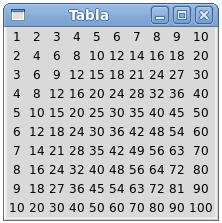
\includegraphics{../../diapos/programas/tkinter/capturas/15.png}

%\section{Cachipún}

En cada ronda del juego del cachipún, los dos competidores deben elegir
entre jugar tijera, papel o piedra.

Las reglas para decidir quién gana la ronda son: tijera le gana a papel,
papel le gana a piedra, piedra le gana a tijera, y todas las demás
combinaciones son empates.

El ganador del juego es el primero que gane tres rondas.

Escriba un programa que pregunte a cada jugador cuál es su jugada,
muestre cuál es el marcador después de cada ronda, y termine cuando uno
de ellos haya ganado tres rondas. Los jugadores deben indicar su jugada
escri\-biendo \lstinline!tijera!, \lstinline!papel! o \lstinline!piedra!.

\begin{lstlisting}[language=testcase]
A: `tijera`
B: `papel`
1 - 0

A: `tijera`
B: `tijera`
1 - 0

A: `piedra`
B: `papel`
1 - 1

A: `piedra`
B: `tijera`
2 - 1

A: `papel`
B: `papel`
2 - 1

A: `papel `
B: `piedra`
3 - 1

A es el ganador
\end{lstlisting}

%\section{Mayusculizador}

Escriba un programa con la siguiente interfaz:

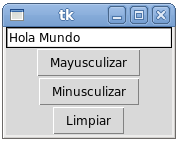
\includegraphics{../../diapos/programas/tkinter/capturas/07-0.png}

Al hacer clic en el botón :kbd:`Mayusculizar`, el texto del campo
superior debe ser convertido a mayúsculas:

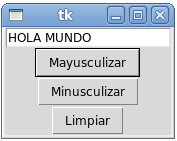
\includegraphics{../../diapos/programas/tkinter/capturas/07-1.png}

Al hacer clic en :kbd:`Minusculizar`, debe ser convertido a minúsculas.

Al hacer clic en :kbd:`Limpiar`, debe borrarse el contenido del campo.

%\section{Buscaminas}

Descarge y pruebe
\href{../../\_static/programas/tkinter/buscaminas.py}{este programa} que
es una implementación del juego Buscaminas.

El juego consiste en descubrir las casillas de un campo minado que no
tienen minas. Al pisar una casilla que tiene una mina, se termina el
juego. El campo minado se representa como una grilla de botones:

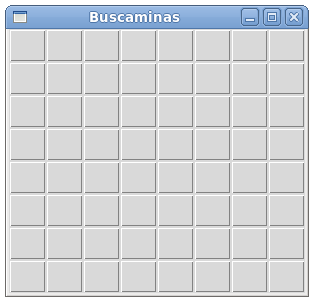
\includegraphics{../../_static/capturas/bm0.png}

Al hacer clic en una casilla no minada, aparece un número que indica en
cuántas de las ocho casillas vecinas hay una mina:

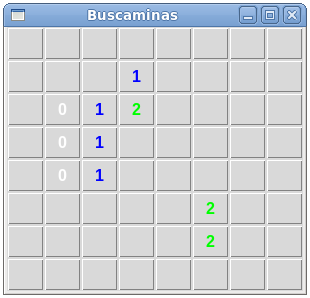
\includegraphics{../../_static/capturas/bm1.png}

Si se hace clic en una mina, el juego termina:

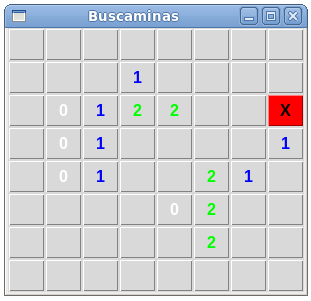
\includegraphics{../../_static/capturas/bm2.png}

\begin{enumerate}
\item
  Modifique el programa para que aparezca un mensaje en la parte
  inferior de la ventana indicando cuántas casillas no minadas faltan
  por ser descubiertas. Cada vez que se haga clic en una nueva casilla,
  el mensaje debe ser actualizado:

  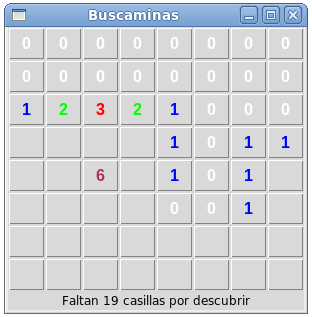
\includegraphics{../../_static/capturas/bm3.png}
\item
  Modifique el programa para que al hacer clic en una mina se muestren
  los contenidos de todas las celdas del campo minado. En la etiqueta
  inferior debe mostrarse el mensaje «¡Perdiste!». La mina que fue
  pisada debe ser indicada con una equis:

  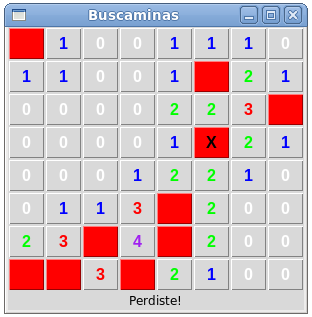
\includegraphics{../../_static/capturas/bm4.png}
\item
  Modifique el programa para que aparezca el mensaje «¡Ganaste!» cuando
  todas las casillas no minadas hayan sido descubiertas.

  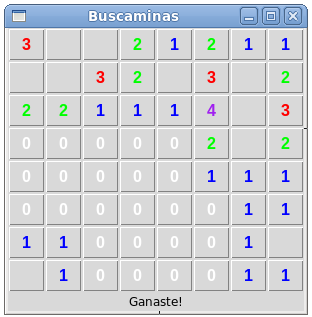
\includegraphics{../../_static/capturas/bm5.png}
\end{enumerate}

%\section{Estadísticas de números}

Escriba un programa que muestre la suma, el promedio, el máximo y el
mínimo de una secuencia de números.

El programa debe verse así:

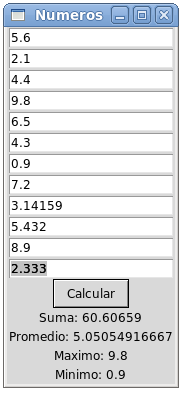
\includegraphics{../../diapos/programas/tkinter/capturas/09.png}

Al hacer clic en :kbd:`Calcular`, deben actualizarse los mensajes en la
parte inferior.

Es mala idea crear los modelos y los campos de entrada de la siguiente
manera:

\begin{lstlisting}
v1 = StringVar()
e1 = Entry(w, textvariable=v1)

v2 = StringVar()
e2 = Entry(w, textvariable=v2)

# ...
\end{lstlisting}

Un buen programador siempre busca la manera de evitar escribir código
repetitivo. Use ciclos y listas con este propósito.

%\documentclass{minimal}
\usepackage[pdftex,active,tightpage]{preview}
\usepackage[utf8]{inputenc}
\usepackage[spanish]{babel}
\usepackage{mathpazo}
\usepackage{tikz}
\usetikzlibrary{calc,arrows,decorations,shapes}
\PreviewEnvironment{tikzpicture}

\begin{document}
\tikzstyle{n}=[xshift=.3cm, yshift=.3cm]
\tikzstyle{a}=[red]
\begin{tikzpicture}[scale=.6]
  %\foreach\i in {0,1,2,3}{
  %  \draw[a] (.1, {0 + .5}) -- ++(4.2, 0);
  %  \draw[a] ({0 + .5}, .1) -- ++(0, 4.2);
  %}

  \draw (0, 0) grid (4, 4);
  \node[n] at (0, 0) {16};
  \node[n] at (1, 0) {3};
  \node[n] at (2, 0) {2};
  \node[n] at (3, 0) {13};

  \node[n] at (0, 1) {5};
  \node[n] at (1, 1) {10};
  \node[n] at (2, 1) {11};
  \node[n] at (3, 1) {8};

  \node[n] at (0, 2) {9};
  \node[n] at (1, 2) {6};
  \node[n] at (2, 2) {7};
  \node[n] at (3, 2) {12};

  \node[n] at (0, 3) {4};
  \node[n] at (1, 3) {15};
  \node[n] at (2, 3) {14};
  \node[n] at (3, 3) {1};

  %\foreach\i in {0,1,2,3}{
  %  \node[n, a] at (4,  \i) { 34};
  %  \node[n, a] at (\i, -1) { 34};
  %}
  %\node[n, a] at (4, 4) { 34};
  %\node[n, a] at (4, -1) { 34};


\end{tikzpicture}
\end{document}

%\section{Buscaminas}

El juego del buscaminas se basa en una grilla rectangular que representa
un campo minado. Algunas de las casillas de la grilla tienen una mina, y
otras no. El juego consiste en descubrir todas las casillas que no
tienen minas.

En un programa, podemos representar un campo de buscaminas como un
arreglo en el que las casillas minadas están marcadas con el valor \(-1\), y
las demás casillas con el valor 0:

\begin{lstlisting}
>>> from numpy import *
>>> campo = array([[ 0,  0, -1,  0,  0,  0,  0,  0],
                   [-1,  0,  0,  0, -1,  0,  0,  0],
                   [ 0,  0,  0,  0, -1,  0,  0, -1],
                   [ 0,  0, -1,  0,  0,  0,  0,  0],
                   [ 0,  0,  0,  0,  0,  0, -1,  0],
                   [ 0, -1,  0,  0, -1,  0,  0,  0],
                   [ 0,  0, -1,  0,  0,  0,  0,  0],
                   [ 0,  0,  0,  0,  0,  0,  0,  0]])
\end{lstlisting}

\begin{enumerate}
\item
  Escriba la función \lstinline!crear_campo(forma, n)!,
  \lstinline!forma! es una tupla \lstinline!(filas, columnas)!, que
  retorne un nuevo campo aleatorio con la forma indicada que tenga
  \lstinline!n! minas.

  Hágalo en los siguientes pasos:

  \begin{enumerate}%[a.]
  \item
    Construya un vector de tamaño \lstinline!filas * columnas! que tenga
    \lstinline!n! veces el valor \(-1\), y a continuación sólo ceros.
  \item
    Importe la función \lstinline!shuffle! desde el módulo
    \lstinline!numpy.random!. Esta función desordena (o «baraja») los
    elementos de un arreglo.
  \item
    Desordene los elementos del vector que creó.
  \item
    Cambie la forma del vector.
  \end{enumerate}

\begin{lstlisting}
>>> crear_campo((4, 4), 5)
array([[-1,  0,  0,  0],
       [ 0,  0,  0,  0],
       [ 0, -1, -1,  0],
       [ 0, -1, -1,  0]])
>>> crear_campo((4, 4), 5)
array([[ 0,  0, -1,  0],
       [ 0,  0,  0, -1],
       [-1,  0,  0,  0],
       [ 0,  0, -1, -1]])
>>> crear_campo((4, 4), 5)
array([[ 0,  0,  0, -1],
       [ 0,  0, -1, -1],
       [-1,  0,  0,  0],
       [ 0,  0, -1,  0]])
\end{lstlisting}
\item
  Al descubrir una casilla no minada, en ella aparece un número, que
  indica la cantidad de minas que hay en sus ocho casillas vecinas.

  Escriba la función \lstinline!descubrir(campo)! que modifique el campo
  poniendo en cada casilla la cantidad de minas vecinas:

\begin{lstlisting}
>>> c = crear_campo((4, 4), 5)
>>> c
array([[ 0,  0, -1, -1],
       [ 0,  0, -1,  0],
       [ 0,  0,  0, -1],
       [ 0,  0,  0, -1]])
>>> descubrir(c)
>>> c
array([[ 0,  2, -1, -1],
       [ 0,  2, -1,  4],
       [ 0,  1,  3, -1],
       [ 0,  0,  2, -1]])
\end{lstlisting}
\end{enumerate}

%\section{Creación de arreglos bidimensionales}

La función \lstinline!arange! retorna un arreglo con números en el rango
indicado:

\begin{lstlisting}
>>> from numpy import arange
>>> a = arange(12)
>>> a
array([ 0,  1,  2,  3,  4,  5,  6,  7,  8,  9, 10, 11])
\end{lstlisting}

A partir del arreglo \lstinline!a! definido arriba, indique cómo obtener
los siguientes arreglos de la manera más simple que pueda:

\begin{lstlisting}
>>> # ???
array([[ 0,  1,  2,  3],
       [ 4,  5,  6,  7],
       [ 8,  9, 10, 11]])
>>> # ???
array([[  0,   1,   4,   9],
       [ 16,  25,  36,  49],
       [ 64,  81, 100, 121]])
>>> # ???
array([[ 0,  4,  8],
       [ 1,  5,  9],
       [ 2,  6, 10],
       [ 3,  7, 11]])
>>> # ???
array([[ 0,  1,  2],
       [ 4,  5,  6],
       [ 8,  9, 10]])
>>> # ???
array([[ 11.5,  10.5,   9.5],
       [  8.5,   7.5,   6.5],
       [  5.5,   4.5,   3.5],
       [  2.5,   1.5,   0.5]])
>>> # ???
array([[100, 201, 302, 403],
       [104, 205, 306, 407],
       [108, 209, 310, 411]])
>>> # ???
array([[100, 101, 102, 103],
       [204, 205, 206, 207],
       [308, 309, 310, 311]])
\end{lstlisting}


%\section{Matrices especiales}

\begin{enumerate}
\item
  Una matriz \lstinline!a! es \emph{simétrica} si para todo par de
  índices \lstinline!i! y \lstinline!j! se cumple que
  \lstinline!a[i, j] == a[j, i]!.

  Escriba la función \lstinline!es_simetrica(a)! que indique si la
  matriz \lstinline!a! es simétrica o no.
  Cree algunas matrices simétricas y otras que no lo sean para probar su
  función.

\item
  Una matriz \lstinline!a! es \emph{antisimétrica} si para todo par de
  índices \lstinline!i! y \lstinline!j! se cumple que
  \lstinline!a[i, j] == -a[j, i]! (note el signo menos).

  Escriba la función \lstinline!es_antisimetrica(a)! que indique si la
  matriz \lstinline!a! es antisimétrica o no.
  Cree algunas matrices antisimétricas y otras que no lo sean para
  probar su función.

\item
  Una matriz \lstinline!a! es \emph{diagonal} si todos sus elementos
  que no están en la diagonal principal tienen el valor cero. Por
  ejemplo, la siguiente matriz es diagonal:

  \[\begin{bmatrix}
  9 & 0 & 0 & 0 \\
  0 & 2 & 0 & 0 \\
  0 & 0 & 0 & 0 \\
  0 & 0 & 0 & -1 \\
  \end{bmatrix}\]

  Escriba la función \lstinline!es_diagonal(a)! que indique si la matriz
  \lstinline!a! es diagonal o no.

\item
  Una matriz \lstinline!a! es \emph{triangular superior} si todos sus
  elementos que están bajo la diagonal principal tienen el valor cero.
  Por ejemplo, la siguiente matriz es triangular superior:

  \[\begin{bmatrix}
  9 & 1 & 0 & 4 \\
  0 & 2 & 8 & -3 \\
  0 & 0 & 0 & 7 \\
  0 & 0 & 0 & -1 \\
  \end{bmatrix}\]

  Escriba la función \lstinline!es_triangular_superior(a)! que indique
  si la matriz \lstinline!a! es trangular superior o no.

\item
  No es dificil deducir qué es lo que es una matriz \emph{triangular
  inferior}. Escriba la función \lstinline!es_triangular_inferior(a)!.
  Para ahorrarse trabajo, llame a \lstinline!es_triangular_superior!
  desde dentro de la función.

\item
  Una matriz es \emph{idempotente} si el resultado del producto
  matricial consigo misma es la misma matriz. Por ejemplo:

  \[\begin{bmatrix}
  2 & -2 & -4 \\
  -1 &  3 &  4 \\
  1 & -2 & -3 \\
  \end{bmatrix}
  \begin{bmatrix}
  2 & -2 & -4 \\
  -1 &  3 &  4 \\
  1 & -2 & -3 \\
  \end{bmatrix}
  =
  \begin{bmatrix}
  2 & -2 & -4 \\
  -1 &  3 &  4 \\
  1 & -2 & -3 \\
  \end{bmatrix}\]

  Escriba la función \lstinline!es_idempotente(a)! que indique si la
  matriz \lstinline!a! es idempotente o no.

\item
  Se dice que dos matrices \(A\) y \(B\) \emph{conmutan} si los
  productos matriciales entre \(A\) y \(B\) y entre \(B\) y
  \(A\) son iguales.

  Por ejemplo, estas dos matrices sí conmutan:

  \[\begin{bmatrix}
  1 & 3 \\ 3 & 2 \\
  \end{bmatrix}
  \begin{bmatrix}
  -1 & 3 \\ 3 & 0 \\
  \end{bmatrix} =
  \begin{bmatrix}
  -1 & 3 \\ 3 & 0 \\
  \end{bmatrix}
  \begin{bmatrix}
  1 & 3 \\ 3 & 2 \\
  \end{bmatrix} =
  \begin{bmatrix}
  8 & 3 \\ 3 & 9 \\
  \end{bmatrix}\]

  Escriba la función \lstinline!conmutan! que indique si dos matrices
  conmutan o no. Pruebe su función con estos ejemplos:
\begin{lstlisting}
>>> a = array([[ 1, 3], [3, 2]])
>>> b = array([[-1, 3], [3, 0]])
>>> conmutan(a, b)
True
>>> a = array([[3, 1, 2], [9, 2, 4]])
>>> b = array([[1, 7], [2, 9]])
>>> conmutan(a, b)
False
\end{lstlisting}
\end{enumerate}

%\section{Informe de producción de gas}

En un informe anual de SansanoGas S.A., el presidente informa a sus
accionistas la cantidad anual de producción de barriles de 50 litros de
lubricantes normal, extra y súper, en sus dos refinerías:

\ctable[pos = H, center, botcap]{llll}
{% notes
}
{% rows
\FL
Refinería & Normal & Extra & Súper
\ML
A & 3000 & 7000 & 2000
\\\noalign{\medskip}
B & 4000 & 500 & 600
\LL
}

Además, informa que en cada barril de 50 litros de lubricante existe la
siguiente composición en litros de aceites finos, alquitrán y grasas
residuales:

\ctable[pos = H, center, botcap]{llll}
{% notes
}
{% rows
\FL
Componente & Normal & Extra & Súper
\ML
Aceites finos & 10 & 5 & 35
\\\noalign{\medskip}
Alquitrán & 15 & 4 & 31
\\\noalign{\medskip}
Grasas residuales & 18 & 2 & 30
\LL
}

\begin{enumerate}
\item
  Escriba la función \lstinline!totales_anuales(a, b)! que reciba como
  parámetros ambas matrices y retorne un arreglo con los totales de
  aceites finos, alquitrán y grasas residuales presentes en la
  producción anual.
\item
  Escriba la función \lstinline!maximo_alquitran(a, b)! que reciba como
  parámetros ambas matrices y retorne el máximo de litros de alquitrán
  consumidos por ambas refinerías.
\item
  Determine cuál es la matriz que entrega el consumo de todos los
  elementos que forman parte de un lubricante, en cada refinería.
\end{enumerate}

%\section{Transmisión de datos}

En varios sistemas de comunicaciones digitales los datos viajan de
manera serial (es decir, uno tras otro), y en bloques de una cantidad
fija de bits (valores 0 o 1). La transmisión física de los datos no
conoce de esta separación por bloques, y por lo tanto es necesario que
haya programas que separen y organicen los datos recibidos.

Los datos transmitidos los representaremos como arreglos cuyos valores
son ceros y unos.

\begin{enumerate}
\item
  Una secuencia de bits puede interpretarse como un número decimal. Cada
  bit está asociado a una potencia de dos, partiendo desde el último
  bit. Por ejemplo, la secuencia 01001 representa al número decimal 9,
  ya que:

  \[0\cdot2^4 +
  1\cdot2^3 +
  0\cdot2^2 +
  0\cdot2^1 +
  1\cdot2^0 = 9\]

  Escriba la función \lstinline!numero_decimal(datos)! que entregue la
  representación decimal de un arreglo de datos:

\begin{lstlisting}
>>> a = array([0, 1, 0, 0, 1])
>>> numero_decimal(a)
9
\end{lstlisting}
\item
  Suponga que el tamaño de los bloques es de cuatro bits. Escriba la
  función \lstinline!bloque_valido(datos)! que verifique que la
  corriente de datos tiene una cantidad entera de bloques:

\begin{lstlisting}
>>> bloque_valido(array([0, 1, 0, 1, 0, 1, 1, 1, 0, 0, 1, 0]))
True
>>> bloque_valido(array([0, 1, 0, 1, 0, 1, 1, 1, 0, 0, 1, 0, 1]))
False
\end{lstlisting}
\item
  Escriba la función \lstinline!decodificar_bloques(datos)! que entregue
  un arreglo con la representación entera de cada bloque. Si un bloque
  está incompleto, esto debe ser indicado con el valor \lstinline!-1!:

\begin{lstlisting}
>>> a = array([0, 1, 0, 1])
>>> b = array([0, 1, 0, 1, 0, 1, 1, 1, 0, 0, 1, 0])
>>> c = array([0, 1, 0, 1, 0, 1, 1, 1, 0, 0, 1, 0, 1])
>>> decodificar_bloques(a)
array([5])
>>> decodificar_bloques(b)
array([5, 7, 2])
>>> decodificar_bloques(c)
array([5, 7, 2, -1])
\end{lstlisting}
\end{enumerate}

%\section{Construcción de una dieta}

\emph{Ejercicio sacado de} {[}Lay97{]}\_.

La dieta Cambridge es una dieta que fue popular en la década de los 80,
y fue el resultado de más de ocho años de trabajo clínico e
investigación de un equipo de científicos liderados por el doctor Alan
H. Howard en la Universidad de Cambridge.

La dieta combina un balance preciso de carbohidratos, proteínas de alta
calidad y grasa, junto con vitaminas, minerales, oligoelementos y
electrolitos. Millones de personas han usado la dieta en años recientes
para bajar rápidamente de peso.

Para alcanzar las proporciones de nutrientes deseadas, el doctor Howard
debió incorporar una gran variedad de comidas en la dieta. Cada comida
provee varios de los nutrientes, pero no en las proporciones correctas.
Por ejemplo, la leche descremada es una buena fuente de proteínas, pero
contiene mucho calcio. Por esto, se usó harina de soya (que tiene poco
calcio) para proveer las proteínas; sin embargo, tiene proporcionalmente
mucha grasa, por lo que se agregó suero de leche a la dieta, que
desafortunadamente contiene muchos carbohidratos\ldots{} como se hace
evidente, el delicado problema de balancear los nutrientes es complejo.

La siguiente tabla muestra el aporte en nutrientes por cada 100 gramos
de cada uno de los tres ingredientes (leche descremada, harina de soya y
suero de leche):

\ctable[pos = H, center, botcap]{llll}
{% notes
}
{% rows
\FL
Nutrientes & LD & HS & SL
\ML
Proteínas & 36 & 51 & 13
\\\noalign{\medskip}
Carbohidratos & 52 & 34 & 74
\\\noalign{\medskip}
Grasas & 0 & 7 & 1.1
\LL
}

La dieta de Cambridge debe proveer 33 gramos de proteínas, 45 gramos de
carbohidratos y 3 gramos de grasa.

Escriba un programa que muestre qué cantidades de ingredientes se debe
usar para satisfacer los requerimientos de la dieta de Cambridge.

%\section{Rotar matrices}

\begin{enumerate}
\item
  Escriba la función \lstinline!rotar90(a)! que retorne el arreglo
  \lstinline!a! rotado 90 grados en el sentido contrario a las agujas
  del reloj:

\begin{lstlisting}
>>> a = arange(12).reshape((3, 4))
>>> a
array([[ 0,  1,  2,  3],
       [ 4,  5,  6,  7],
       [ 8,  9, 10, 11]])
>>> rotar90(a)
array([[ 3,  7, 11],
       [ 2,  6, 10],
       [ 1,  5,  9],
       [ 0,  4,  8]])
\end{lstlisting}

  Hay dos maneras de hacerlo: la larga (usando ciclos anidados) y la
  corta (usando operaciones de arreglos). Trate de hacerlo de las dos
  maneras.
\item
  Escriba las funciones \lstinline!rotar180(a)! y
  \lstinline!rotar270(a)!:

\begin{lstlisting}
>>> rotar180(a)
array([[11, 10,  9,  8],
       [ 7,  6,  5,  4],
       [ 3,  2,  1,  0]])
>>> rotar270(a)
array([[ 8,  4,  0],
       [ 9,  5,  1],
       [10,  6,  2],
       [11,  7,  3]])
\end{lstlisting}

  Hay tres maneras de hacerlo: la larga (usando ciclos anidados), la
  corta (usando operaciones de arreglos) y la astuta. Trate de hacerlo
  de las tres maneras.
\item
  Escriba el módulo \lstinline!rotar.py! que contenga estas tres
  funciones. %Le será útil más adelante:

\begin{lstlisting}
>>> from rotar import rotar90
>>> a = array([[6, 3, 8],
...            [9, 2, 0]])
>>> rotar90(a)
array([[8, 0],
       [3, 2],
       [6, 9]])
\end{lstlisting}
\end{enumerate}

%\chapter{Calculadora simple}

El siguiente programa es una calculadora simple:

Al ejecutar el programa, primero uno ingresa la operación que será
aplicada, que puede ser:

\ctable[pos = H, center, botcap]{ll}
{% notes
}
{% rows
\FL
Signo & Operación
\\\noalign{\medskip}
------- & ---------------
\\\noalign{\medskip}
\lstinline!+! & Suma
\\\noalign{\medskip}
\lstinline!-! & Resta
\\\noalign{\medskip}
\lstinline!*! & Multiplicación
\\\noalign{\medskip}
\lstinline!/! & División
\\\noalign{\medskip}
\lstinline!^! & Potencia
\LL
}

La multiplicación también puede ser indicada con una \lstinline!x!
minúscula.

A continuación, se debe ingresar los dos operandos. Finalmente, el
programa muestra el resultado de la operación.

Escriba, compile y ejecute este programa.

En este programa puede ver que es posible asignar un valor inicial a una
variable al momento de declararla:

\begin{lstlisting}
float resultado = 1.0;
int valido = 1;
\end{lstlisting}

También note que tanto en el \lstinline!if! como en el \lstinline!else!
del final se ha omitido los paréntesis de llave (\lstinline!{}!) ya que
en ambos casos hay incluída solamente una única sentencia.

\section{Definición de funciones}

Al principio del programa, se ha definido una función llamada
\lstinline!potencia!. Ella recibe como parámetros la base (un número
real) y el exponente (un entero), y retorna el resultado de elevar la
base al exponente.

En C no existe un operador «elevado a» (como el \lstinline!**! de
Python), por lo que sí es útil definir una función como ésta.

Es necesario especificar explícitamente cuál será el tipo del valor
retornado (en este caso \lstinline!float!) y los tipos de cada uno de
los parámetros (en el ejemplo, \lstinline!float! e \lstinline!int!).

Las variables declaradas dentro de la función se llaman
\textbf{variables locales}. Estas variables comienzan a existir al
momento de llamar a la función, y desaparecen cuando la función termina.
Son invisibles desde fuera de la función.

En nuestro programa, las dos funciones \lstinline!main! y
\lstinline!potencia! tienen una variable local llamada
\lstinline!resultado!. Ambas variables son distintas, y sus valores
respectivos están almacenados en regiones diferentes de la memoria.

\section{Tipo char}

El tipo \lstinline!char! se usa para representar caracteres (símbolos)
solitarios. La variable \lstinline!op! que almacena la operación es de
este tipo.

Un valor de tipo \lstinline!char! se representa en un programa entre
comillas simples. Por ejemplo, el signo más está representado como
\lstinline!'+'!.

Técnicamente, los valores de tipo \lstinline!char! son números enteros
que están comprendidos entre −128 y 127. Cada número está asociado a un
caracter a través de la
\href{http://es.wikipedia.org/wiki/C\%C3\%B3digo\_ASCII\#Caracteres\_imprimibles\_ASCII}{tabla
ASCII}. Los enteros y los caracteres asociados son intercambiables; por
ejemplo, la expresión \lstinline!'m' == 109! es evaluada como verdadera.

No hay que confundir un caracter con un string de largo uno:
\lstinline!'a'! y \lstinline!"a"! son dos cosas distintas.

\section{Sentencia switch}

El \textbf{switch} es una sentencia de control condicional que permite
indicar qué hacer si el resultado de una expresión es igual a alguno de
ciertos valores constantes indicados

Un ejemplo de uso de \lstinline!switch! es el siguiente:

\begin{lstlisting}
switch (expresion) {
    case 1:
        /* que hacer cuando expresion == 1 */

    case 2:
        /* que hacer cuando expresion == 2 */

    default:
        /* que hacer cuando la expresion no es igual
         * a ninguno de los casos anteriores */
}
\end{lstlisting}

Cuando el resultado de la expresión es igual a alguno de los valores
indicados, la ejecución del programa salta al \lstinline!case! con ese
valor. Si el valor con el resultado no existe, salta a
\lstinline!default!.

Hay que tener cuidado con una característica extraña del
\lstinline!switch!: cuando se cumple un caso, los casos que vienen a
continuación también se ejecutan. En este ejemplo:

\begin{itemize}
\item
  si \lstinline!expresion == 1!, el programa saltará a
  \lstinline!case 1!, y luego continuará con \lstinline!case 2! y
  \lstinline!default!;
\item
  si \lstinline!expresion == 2!, el programa saltará a
  \lstinline!case 2!, y luego continuará con \lstinline!default!;
\item
  si \lstinline!expresion! no es ni 1 ni 2, el programa saltará a
  \lstinline!default!.
\end{itemize}

Para evitar que los casos siguientes sean ejecutados, debe ponerse un
\lstinline!break! al final de cada caso. Esto es lo que se hizo en el
programa de la calculadora.

\section{Conversión de tipos}

El segundo parámetro de la función \lstinline!potencia! es entero, pero
los operandos ingresados por el usuario son almacenados como números
reales.

Para convertir el exponente de real a entero, basta con anteponer al
valor el tipo entre paréntesis.

En este caso particular, la conversión se hace truncando los decimales
del número real. Así, si \lstinline!y! vale \lstinline!5.9!, entonces
\lstinline!(int) y! vale \lstinline!5!. Para conversiones entre otros
tipos, se siguen otras reglas diferentes.

En inglés, el nombre de esta operación es \emph{cast}. Posiblemente
usted escuche más de una vez a alguien refiriéndose a esta operación
como «castear».

\section{Ejercicios}

Modifique el programa de modo que soporte una nueva operación: obtener
el \href{http://es.wikipedia.org/wiki/Coeficiente\_binomial}{coeficiente
binomial} entre \lstinline!x! e \lstinline!y!. Esta operación debe ser
indicada con el símbolo \lstinline!b!:

El coeficiente binomial es una operación entre números enteros. Tenga
cuidado y use conversiones apropiadas.

%\section{Series de tiempo}

\emph{Este problema apareció en el certamen 3 del primer semestre de
2011.}

Una \textbf{serie de tiempo} es una secuencia de valores numéricos
obtenidos al medir algún fenómeno cada cierto tiempo. Algunos ejemplos
de series de tiempo son: el precio del dólar en cada segundo, el nivel
medio mensual de concentración de `CO\_2` en el aire y las temperaturas
máximas anuales de una ciudad. En un programa, los valores de una serie
de tiempo se pueden guardar en un arreglo.

Las \textbf{medias móviles} con retardo \emph{p} de una serie de tiempo
son la secuencia de todos los promedios de \emph{p} valores consecutivos
de la serie.

Por ejemplo, si los valores de la serie son `\{5, 2, 2, 8, -4, -1, 2\}`
entonces las medias móviles con retardo 3 son: `frac\{5 + 2 + 2\}\{3\}`,
`frac\{2 + 2 + 8\}\{3\}`, `frac\{2 + 8 - 4\}\{3\}`, `frac\{8 - 4 -
1\}\{3\}` y `frac\{-4 -1 + 2\}\{3\}`.

\begin{enumerate}
\item
  Escriba la función \lstinline!medias_moviles(serie, p)! que retorne el
  arreglo de las medias móviles con retardo \emph{p} de la serie:

\begin{lstlisting}
>>> s = array([5, 2, 2, 8, -4, -1, 2])
>>> medias_moviles(s, 3)
array([ 3,  4,  2,  1, -1])
\end{lstlisting}
\item
  Las \textbf{diferencias finitas} de una serie de tiempo son la
  secuencia de todas las diferencias entre un valor y el anterior.

  Por ejemplo, si los valores de la serie son `\{5, 2, 2, 8, -4, -1,
  2\}` entonces las diferencias finitas son: `(2 - 5)`, `(2 - 2)`, `(8 -
  2)`, `(-4 - 8)`, `(-1 + 4)` y `(2 + 1)`.

  Escriba la función \lstinline!diferencias_finitas(serie)! que retorne
  el arreglo de las diferencias finitas de la serie:

\begin{lstlisting}
>>> s = array([5, 2, 2, 8, -4, -1, 2])
>>> diferencias_finitas(s)
array([ -3,   0,   6, -12,   3,   3])
\end{lstlisting}
\end{enumerate}

%\section{Barman}

Para preparar aperitivos, un barman almacena en tres baldes distintas
medidas de vino, ginebra y jugo de limón, según la siguiente tabla:

\ctable[pos = H, center, botcap]{llll}
{% notes
}
{% rows
\FL
Balde & Vino & Ginebra & Jugo de limón
\ML
A & 20 & 30 & 50
\\\noalign{\medskip}
B & 30 & 20 & 60
\\\noalign{\medskip}
C & 30 & 30 & 32
\LL
}

Por otro lado, se tiene la información de los precios por litro de cada
líquido:

\ctable[pos = H, center, botcap]{ll}
{% notes
}
{% rows
\FL
Líquido & Precio
\ML
Vino & 5
\\\noalign{\medskip}
Ginebra & 45
\\\noalign{\medskip}
Jugo de limón & 10
\LL
}

\begin{enumerate}
\item
  Escriba un programa que muestre cuál es el precio de cada uno de los
  baldes.
\item
  Escriba un programa que muestre el precio total de 10 baldes A, 4
  baldes B y 5 baldes C.
\end{enumerate}

%\documentclass{minimal}
\usepackage[pdftex,active,tightpage]{preview}
\usepackage[utf8]{inputenc}
\usepackage[spanish]{babel}
\usepackage{tikz}
\usepackage{mathpazo}
\usetikzlibrary{calc,shapes,arrows}

\newcounter{row}
\newcounter{col}

\newcommand\setrow[9]{
  \setcounter{col}{1}
  \foreach \n in {#1, #2, #3, #4, #5, #6, #7, #8, #9} {
    \node[anchor=center] at ({{\value{col}} - 0.5}, {9.5 - {\value{row}}}) {\n};
    \stepcounter{col}
  }
  \stepcounter{row}
}

\begin{document}
\begin{preview}
\begin{tikzpicture}[scale=.5]

  \begin{scope}
    \draw (0, 0) grid (9, 9);
    \draw[very thick, scale=3] (0, 0) grid (3, 3);

    \setcounter{row}{1}
    \setrow { }{2}{ }  {5}{ }{1}  { }{9}{ }
    \setrow {8}{ }{ }  {2}{ }{3}  { }{ }{6}
    \setrow { }{3}{ }  { }{6}{ }  { }{7}{ }

    \setrow { }{ }{1}  { }{ }{ }  {6}{ }{ }
    \setrow {5}{4}{ }  { }{ }{ }  { }{1}{9}
    \setrow { }{ }{2}  { }{ }{ }  {7}{ }{ }

    \setrow { }{9}{ }  { }{3}{ }  { }{8}{ }
    \setrow {2}{ }{ }  {8}{ }{4}  { }{ }{7}
    \setrow { }{1}{ }  {9}{ }{7}  { }{6}{ }

    \node[anchor=center] at (4.5, -0.5) {Sudoku sin resolver};
  \end{scope}

  \begin{scope}[xshift=12cm]
    \draw (0, 0) grid (9, 9);
    \draw[very thick, scale=3] (0, 0) grid (3, 3);

    \setcounter{row}{1}
    \setrow { }{2}{ }  {5}{ }{1}  { }{9}{ }
    \setrow {8}{ }{ }  {2}{ }{3}  { }{ }{6}
    \setrow { }{3}{ }  { }{6}{ }  { }{7}{ }

    \setrow { }{ }{1}  { }{ }{ }  {6}{ }{ }
    \setrow {5}{4}{ }  { }{ }{ }  { }{1}{9}
    \setrow { }{ }{2}  { }{ }{ }  {7}{ }{ }

    \setrow { }{9}{ }  { }{3}{ }  { }{8}{ }
    \setrow {2}{ }{ }  {8}{ }{4}  { }{ }{7}
    \setrow { }{1}{ }  {9}{ }{7}  { }{6}{ }

    \node[anchor=center] at (4.5, -0.5) {Sudoku resuelto};
    \begin{scope}[blue, font=\sffamily\slshape]
      \setcounter{row}{1}
      \setrow {4}{ }{6}  { }{7}{ }  {3}{ }{8}
      \setrow { }{5}{7}  { }{9}{ }  {1}{4}{ }
      \setrow {1}{ }{9}  {4}{ }{8}  {2}{ }{5}

      \setrow {9}{7}{ }  {3}{8}{5}  { }{2}{4}
      \setrow { }{ }{3}  {7}{2}{6}  {8}{ }{ }
      \setrow {6}{8}{ }  {1}{4}{9}  { }{5}{3}

      \setrow {7}{ }{4}  {6}{ }{2}  {5}{ }{1}
      \setrow { }{6}{5}  { }{1}{ }  {9}{3}{ }
      \setrow {3}{ }{8}  { }{5}{ }  {4}{ }{2}
    \end{scope}
  \end{scope}

\end{tikzpicture}
\end{preview}
\end{document}

%\section{Contador de clics}

Escriba un programa con la siguiente interfaz:

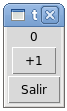
\includegraphics{../../diapos/programas/tkinter/capturas/06-0.png}

Cada vez que se haga clic en el botón :kbd:`+1`, el número en la parte
superior debe aumentar en uno.

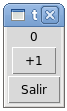
\includegraphics{../../diapos/programas/tkinter/capturas/06-0.png}

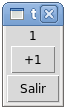
\includegraphics{../../diapos/programas/tkinter/capturas/06-1.png}

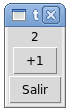
\includegraphics{../../diapos/programas/tkinter/capturas/06-2.png}

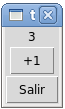
\includegraphics{../../diapos/programas/tkinter/capturas/06-3.png}

Al hacer clic en el botón :kbd:`Salir`, el programa debe terminar.

%\section{Producción de autos}

Una fábrica de autos produce tres modelos: sedán, camioneta y económico.
Cada auto necesita para su producción materiales, personal, impuestos y
transporte. Los costos en unidades por cada concepto son los siguientes:

\ctable[pos = H, center, botcap]{llll}
{% notes
}
{% rows
\FL
(Costos) & Sedán & Camioneta & Económico
\ML
Material & 7 & 8 & 5
\\\noalign{\medskip}
Personal & 10 & 9 & 7
\\\noalign{\medskip}
Impuestos & 5 & 3 & 2
\\\noalign{\medskip}
Transporte & 2 & 3 & 1
\LL
}

Semanalmente, se producen 60 sedanes, 40 camionetas y 90 económicos.

Los costos de una unidad de material, personal, impuestos y transporte
son respectivamente 5, 15, 7 y 2.

Escriba un programa que muestre:

\begin{itemize}
\item
  las unidades semanales necesarias de material, personal, impuestos y
  transporte,
\item
  el costo total de un auto de cada modelo,
\item
  el costo total de la producción semanal.
\end{itemize}

%\section{Conversor de temperatura}

Escriba un programa para convertir grados Fahrenheit a Celsius. El
programa debe verse así:

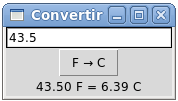
\includegraphics{../../diapos/programas/tkinter/capturas/08.png}

Al hacer clic en el botón, debe actualizarse el mensaje en la parte
inferior de la ventana.

%\section{Migración de poblaciones}

\emph{Ejercicio sacado de} {[}Lay97{]}\_.

Estudios demográficos muestran que, cada año, el 5\% de la población de
una ciudad se muda a los suburbios (y el 95\% se queda), mientras que el
3\% de la población de los suburbios se muda a la ciudad (y el 97\% se
muda).

Estos datos pueden ser representados en una \textbf{matriz de
migración}:

\[M =
\frac{1}{100}
\begin{bmatrix}
95 &  3 \\
5 & 97 \\
\end{bmatrix}\]

\begin{enumerate}
\item
  Escriba un programa que pregunte al usuario cuáles son las poblaciones
  de la ciudad y los suburbios en el año 2011, y entregue una tabla con
  las poblaciones proyectadas para los siguientes 10 años:
\item
  Considere ahora la siguiente variación. Suponga que todos los años hay
  14000 personas que se mudan a la ciudad desde fuera de la región (no
  desde los suburbios) y 9000 personas abandonan la región; además, hay
  13000 personas que se mudan anualmente a los suburbios desde fuera de
  la ciudad.

  Modifique el programa anterior para resolver este problema.
\end{enumerate}



  \documentclass[12pt,spanish,letterpaper]{article}
\usepackage[utf8]{inputenc}
\usepackage{babel}
\usepackage{fullpage}
\usepackage{listings}
\usepackage{mathpazo}
\usepackage{enumitem}
\usepackage{courier}
\usepackage{xcolor}
\usepackage{textcomp}
\usepackage{amsmath}
\usepackage{amssymb}
\usepackage{tikz}
\usepackage{fancyhdr}
\usepackage{graphics}

\newcommand{\titulo}{Control en línea, semana \#5}
\newcommand{\onelinerule}{\rule[2.3ex]{0pt}{0pt}}
\newcommand{\twolinerule}{\rule[6.2ex]{0pt}{0pt}}
\newcommand{\respuesta}{\framebox[\textwidth]{\twolinerule}}
\newcommand{\nombre}{%
  \begin{tikzpicture}[xscale=.4,yscale=.7]
    \draw (0, 0) rectangle (22, 1);
  \end{tikzpicture}%
}
%\newcommand{\rol}   {\framebox[0.3\textwidth]{\onelinerule}}
\newcommand{\rol}{%
  \begin{tikzpicture}[xscale=.4,yscale=.7]
    \draw[gray!40] ( 0, 0) grid      ( 9, 1);
    \draw          ( 0, 0) rectangle ( 9, 1);
    \draw          (10, 0) rectangle (11, 1);
    \draw (9 + .2, .5) -- (10 - .2, .5);
  \end{tikzpicture}%
}
\newcommand{\li}{\lstinline}
\providecommand{\pond}[1]{[{\small\textbf{#1\%}}]}

\lstdefinelanguage{py}{%
  classoffset=0,%
    morekeywords={%
      False,class,finally,is,return,None,continue,for,lambda,try,%
      True,def,from,nonlocal,while,and,del,global,not,with,print,%
      as,elif,if,or,yield,assert,else,import,pass,break,except,in,raise},%
    keywordstyle=\color{black!80}\bfseries,%
  classoffset=1,
    morekeywords={int,float,str,abs,len,raw_input,exit,range,min,max,%
      set,dict,tuple,list,bool,complex,round,sum,all,any,zip,map,filter,%
      sorted,reversed,dir,file,frozenset,open,%
      array,zeros,ones,arange,linspace,eye,diag,dot},
    keywordstyle=\color{black!50}\bfseries,%
  classoffset=0,%
  sensitive=true,%
  morecomment=[l]\#,%
  morestring=[b]',%
  morestring=[b]",%
  stringstyle=\em,%
}

\lstdefinelanguage{testcase}{%
  moredelim=[is][\bfseries]{`}{`},%
  backgroundcolor=\color{gray!20},%
}

\lstdefinelanguage{file}{%
  frame=single,%
}

\lstset{language=py}
\lstset{basicstyle=\ttfamily}
\lstset{columns=fixed}
\lstset{upquote=true}
\lstset{showstringspaces=false}
\lstset{rangeprefix=\#\ }
\lstset{includerangemarker=false}

\newlist{certamen}{enumerate}{1}
\setlist[certamen]{%
  label=\arabic*.,
  font=\LARGE\bfseries,%
  labelindent=-.5in,%
  leftmargin=0pt,%
  labelsep=1em%
}


\pagestyle{fancy}
\lhead{\Large\bfseries Programación---\titulo}
\chead{}\rhead{}\lfoot{}\cfoot{}\rfoot{}
\renewcommand{\headrulewidth}{0pt}
\addtolength{\headheight}{7ex}
\headsep=2ex



\begin{document}

  Escriba una función \li!cuenta_digito(d, n)!
  que retorne la cantidad de veces
  que aparece el dígito \li!d!
  en el número \li!n!:

  \lstinputlisting{c-caso1.py}

  A continuación,
  escriba un función \li!siguiente_con_digitos(d, c, m)!
  que retorne el primer número mayor que \li!m!
  en el que el dígito \li!d! aparece por lo menos \li!c! veces:

  \lstinputlisting{c-caso2.py}

  La función \li!siguiente_con_digitos!
  debe llamar a \li!cuenta_digito!.
  Ambas funciones deben estar en el mismo archivo,
  y deben tener exactamente los nombres indicados en el enunciado.

\end{document}


\end{document}
